
%\documentclass[print]{thesis}    % print version with black links
\documentclass[]{thesis}         % pdf version with colored links
%\documentclass[draft]{thesis}    % no images

\hypersetup{
    pdftitle = {Lexicon Formation in Autonomous Robots},
    pdfauthor = {Martin Loetzsch}
}

\begin{document}



\sffamily

\centerline{\bfseries\Large Lexicon Formation in Autonomous Robots}

\vspace{1.5cm}

\large 
\centerline{D I S S E R T A T I O N}

\vspace{0.2cm}

\centerline{zur Erlangung des akademischen Grades}

\vspace{0.2cm}

\centerline{Dr. rer. nat.}
\centerline{im Fach Informatik}

\vspace{0.8cm}

\centerline{eingereicht an der}

\vspace{0.2cm}

\centerline{Mathematisch-Naturwissenschaftlichen Fakultät II}
\centerline{Humboldt-Universität zu Berlin}

\vspace{0.8cm}

\centerline{von}
\centerline{\sffamily Martin Loetzsch}
\centerline{20/11/1977 Neustrelitz}


\vspace{2cm}

\rmfamily

Präsident der Humboldt-Universität zu Berlin:

Prof. Dr. Jan-Hendrik Olbertz

\vspace{0.5cm}

Dekan der Mathematisch-Naturwissenschaftlichen Fakultät II:

Prof. Dr. Elmar Kulke

\vspace{0.5cm}


Gutachter:

1. Prof. Dr. i. R. Hans-Dieter Burkhard

2. Prof. Dr. Luc Steels

3. Prof. Dr. Raul Rojas


\vspace{0.5cm}

eingereicht am: 5.6.2013

Tag der mündlichen Prüfung: 19.2.2014

\normalsize

\cleardoublepage

%%% Local Variables: 
%%% mode: latex
%%% TeX-master: "phd-thesis"
%%% End: 



~\\



\begin{addmargin}[1.2cm]{1.2cm}
{\Large\sffamily\bfseries Abstract}
\vspace{0.5cm}

\noindent ``The meaning of a word is its use in the language''. In the
first half of the 20th century Ludwig Wittgenstein introduced this
idea into philosophy and especially in the last few decades, related
disciplines such as psychology and linguistics started embracing the
view that that natural language is a dynamic system of arbitrary and
culturally learnt conventions. From the end of the nineties on,
researchers around Luc Steels transferred this notion of communication
to the field of artificial intelligence by letting software agents and
later robots play so-called language games in order to self-organize
communication systems without requiring prior linguistic or conceptual
knowledge. Continuing and advancing that research, the work presented
in this thesis investigates lexicon formation in humanoid robots,
i.e. the emergence of shared lexical knowledge in populations of
robotic agents. Central to this is the concept of referential
uncertainty, which is the difficulty of guessing a previously unknown
word from the context. First in a simulated environments and later
with physical robots, this work starts from very simple lexicon
formation models and then systematically analyzes how an increasing
complexity in communicative interactions leads to an increasing
complexity of representations and learning mechanisms. We evaluate
lexicon formation models with respect to their robustness, scaling and
their applicability to robotic interaction scenarios and one result of
this work is that the predominating approaches in the literature do
not scale well and are not able to cope with the challenges stemming
from grounding words in the real-world perceptions of physical
robots. In order to overcome these limitations, we present an
alternative lexicon formation model and evaluate its performance.
\end{addmargin}

\cleardoublepage




% ~\\

% \begin{addmargin}[1.2cm]{1.2cm}

% {\Large\sffamily\bfseries Zusammenfassung}
% \vspace{0.5cm}

% \noindent ``Die Bedeutung eines Wortes ist sein Gebrauch in der
% Sprache''. Ludwig Wittgenstein führte diese Idee in der ersten Hälfte
% des 20. Jahrhunderts in die Philosophie ein und in verwandten
% Disziplinen wie der Psychologie und Linguistik setzte sich vor allem
% in den letzten Jahrzehnten die Ansicht durch, dass natürliche Sprache
% ein dynamisches System arbiträrer und kulturell gelernter Konventionen
% ist. Forscher um Luc Steels übertrugen diesen Sprachbegriff seit Ende
% der 90er Jahre auf das Gebiet der Künstlichen Intelligenz, indem sie
% zunächst Software-Agenten und später Robotern mittels sogenannter
% Sprachspiele gemeinsame Kommunikationssysteme bilden liessen, ohne
% dass Agenten im Voraus mit linguistischem und konzeptionellen Wissen
% ausgestattet werden. Die vorliegende Arbeit knüpft an diese Forschung
% an und untersucht vertiefend die Selbstorganisation von geteiltem
% lexikalischen Wissen in humanoiden Robotern. Zentral ist dabei das
% Konzept der ``referential uncertainty'', d.h. die Schwierigkeit, die
% Bedeutung eines bisher unbekannten Wortes aus dem Kontext zu
% erschliessen. Ausgehend von sehr einfachen Modellen der Lexikonbildung
% untersucht die Arbeit zunächst in einer simulierten Umgebung und
% später mit physikalischen Robotern systematisch, wie zunehmende
% Komplexität kommunikativer Interaktionen komplexere Lernmodelle und
% Reprä\-sentationen erfordert. Ein Ergebnis der Evaluierung der Modelle
% hinsichtlich Robustheit und Übertragbarkeit auf Interaktionszenarien
% mit Robotern ist, dass die in der Literatur vorwiegenden
% selektionistischen Ansätze schlecht skalieren und mit der zusätzlichen
% Herausforderung einer Verankerung in visuellen Perzeptionen echter
% Roboter nicht zurecht kommen. Davon ausgehend wird ein alternatives
% Modell vorgestellt.
% \end{addmargin}

% \cleardoublepage

\normalsize

%%% Local Variables: 
%%% mode: latex
%%% TeX-master: "thesis"
%%% End: 


%% \tableofcontents


%% \part{Introduction}
%% 
\chapter{Investigating the emergence of communication systems}

One of the most important findings of cognitive science has been the
insight that even supposedly simple mental tasks such as recognizing
objects or performing arm movements are actually the result of a
complex interplay between a highly interwoven network of cognitive
processes, the body, and the physical world and the social
environment. And it turned out that the capability to use symbolic
language -- one of the few features (if not the only) that sets us
apart from the animal kingdom -- is not an isolated mental skill
either but relies on and emerges from large parts of the cognitive
apparatus that is available to us. Progress in neuroscience and
related areas has given us quite some understanding of the underlying
mechanisms of perception, motor control, memory, etc., but theories of
``how language works'' are just beginning to emerge.

Coming from an artificial intelligence background, we want to explore
the question of ``how language could work'' by designing artificial
robotic agents that learn to communicate with each other about things
in their environment. This involves finding solutions to a wide
variety of challenges: how can we build robots that are able to
perceive the world, that construct persistent mental representations
of what they experience, that interact socially with each other and --
most importantly -- that have the capability to communicate? Endowing
our agents with a ``capability to communicate'' does not mean that we
will give them a pre-existing language. We will instead investigate
how they can self-organize communication systems through local
conversations, i.e. how they can agree on a shared language in order
to communicate successfully. 

The work presented in this thesis will not cover the whole complexity
of human language (which would include grammar, morphology, etc.) but
we will focus on lexicon formation. That means we will show how agents
can learn names for objects in their environment (i.e. words similar
to proper names such as ``John'', adjectives such as ``green'' and
nouns such as ``block'') from each other. We will start from very
simple models and then demonstrate how the increased complexity of
communicative challenges and agent architectures leads to more complex
word learning models. In series of controlled experiments we will
evaluate the performance of these models as well as the influence of
internal and external factors -- both in simulated environments where
agents have idealized abstract perceptions of the world and with
actual physical robots, which will allow us to analyse the impact of
embodiment on the dynamics of the interactions.


\begin{figure}[t]
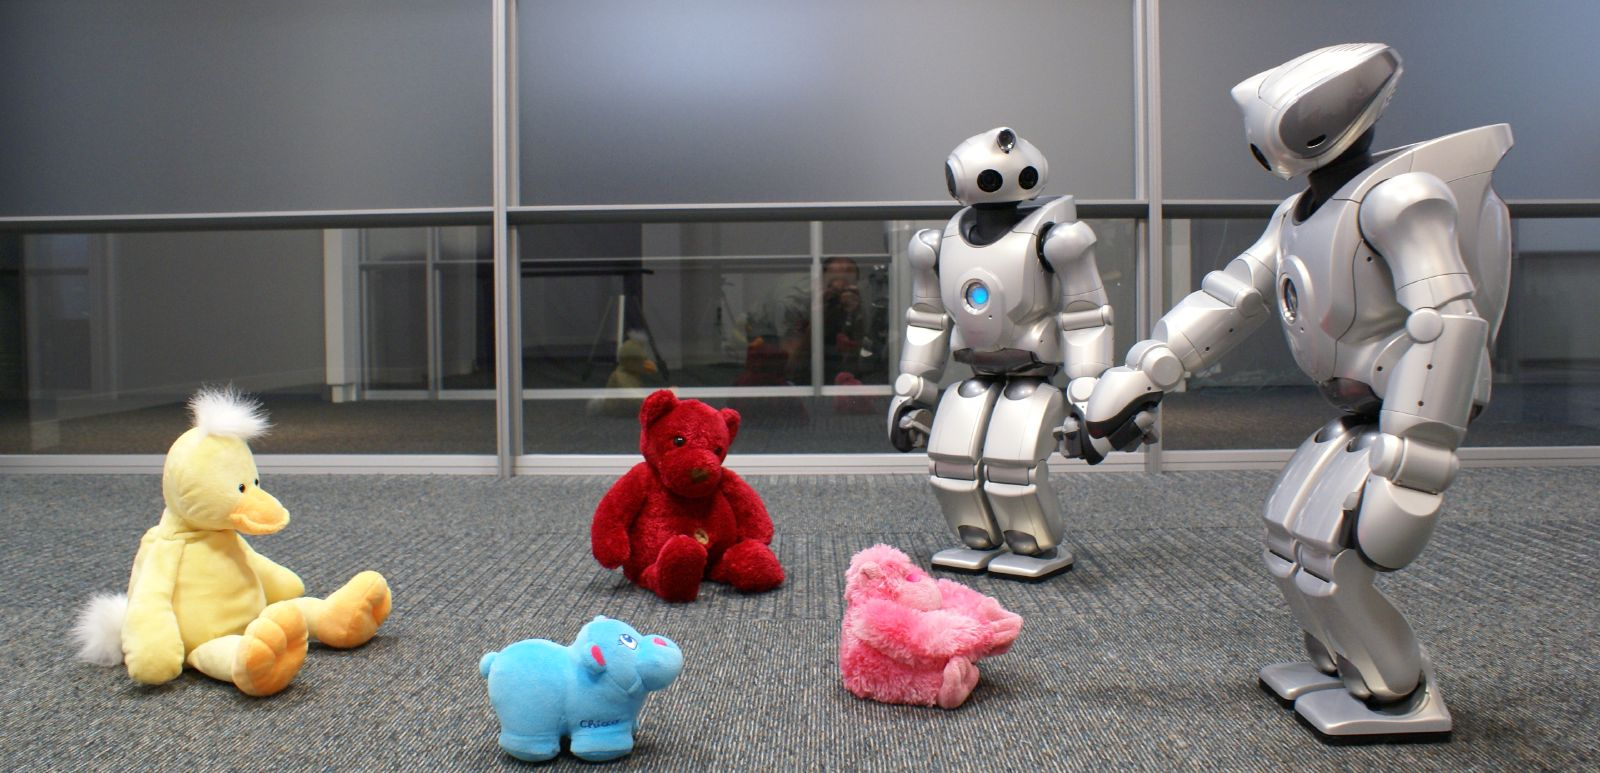
\includegraphics[width=\textwidth]{figures/photo-2-qrios-with-4-toys}
\caption{Example of a communicative interaction between two
  agents. The robots perceive objects in their shared environment
  through their built-in cameras and subsequently engage in a
  conversation about one of the objects. Over the course of repeated
  such interactions, populations of agents are able to coordinate
  their conceptual repertoires for recognizing and classifying objects
  as well as a shared language for communicating about them.}
\label{f:photo-2-qrios-with-4-toys}
\end{figure}

Let us give an example of how such an experiment could look
like. Figure \ref{f:photo-2-qrios-with-4-toys} shows two robotic
agents that are placed in an office environment with a set of toy
objects in front of them. The robot at the right will take the role of
the speaker and the other the role of a hearer. The communicative goal
of the speaker will be to draw the attention of the hearer to one of
the objects (e.g. the pink monkey). For this, he will first have to
classify the visual experience of the object with respect to how
similar it is to mental representations of previously experienced
objects (i.e. he has to recognize the pink monkey as a {\tt monkey},
as something {\tt pink}, as {\tt the closest object}, etc.) -- or, in
case he has never before seen a similar looking object, construct such
a representation. Then, the speaker will use words from his own
private linguistic inventory that he associates with the recognized
concepts and that he thinks of will serve his communicative goal best
(and again invent words when he does not know how to express the
concepts). The hearer will then try to interpret the utterance using
his own sensory experience of the scene and his own private conceptual
and linguistic repertoires. The hearer infers the communicative goal
of the speaker by finding the object that fits best the concepts
associated to the words heard. It can of course happen that both
agents connect different meanings to the words of the utterance. To
avoid potential misunderstandings, the hearer points to the object
that he understood and the speaker will either signal a confirmation
(if the object pointed at was indeed the one he intended) or otherwise
point to the correct object. It might furthermore happen that the
hearer does not know one of the words at all or is otherwise not able
to infer the topic of the conversation -- also in this case the
speaker will point to the object he had in mind, allowing the hearer
to learn the meaning of the word.



For taking part in such interactions, the robots certainly need to be
endowed with a powerful set of mental capabilities and we will analyze
what these have to be. Building robotic systems that are able to
self-organize linguistic communication systems from scratch is a very
exciting -- and also extraordinarily difficult -- engineering
challenge. It involves dealing with high levels of complexity in the
interaction of the different cognitive processes and we will explore
how (by going from simple models to more advanced ones) the complexity
of different dynamics can be handled and explained. In addition to
that, we will take inspiration from psychologists and linguists such
as
\cite{tomasello03constructing,tomasello99cultural,tomasello08origins,bloom00how-children,bowerman01language}
who discuss human intelligence and language as a result of
capabilities for engaging in social activities, for constructing
mental representations about the world and other general learning
mechanisms. We will demonstrate how their theories about language and
cognition can be operationalized in computational models and
additionally use these models to verify hypotheses coming out of these
research fields. In this chapter we will lay out the theoretical
foundations for this work. Chapter \ref{c:building-blocks} will
introduce the methods and tools that were used for our experiments and
then Chapter \ref{c:thesis-overview} will sum up this introduction by
giving an overview of the work.\\

\noindent This thesis' investigations are a truly multidisciplinary endeavour:
we will borrow ideas from artificial intelligence, robotics, 
psychology, linguistics and philosophy and -- although our
contribution is clearly rooted in artificial intelligence -- we also
want to be relevant to all of these disciplines. Before we begin, let
us set the stage by outlining the theoretical and methodological basis
for our experiments as well as embed the work in the literature (those
readers who are familiar with the research field of artificial
language evolution can safely skip this part and continue with Chapter
\ref{c:building-blocks}).



\section{Basic assumptions}
\label{s:basic-assumptions}

The question of what language is, how it is learnt, how it changes,
which cognitive mechanisms are involved, etc. (in short: how it works)
is far from being settled -- in fact, the study of language is
probably the field within the cognitive sciences with the biggest
variety of competing theories. Many ideas that were considered to be
state of the art in the recent past are nowadays seen as outdated by
younger scholars but still receive attention and support by major
parts of the scientific community. Due to this absence of a common
theoretical basis, it is very likely that the particular view on
language taken in thesis is not shared by many linguists,
psychologists and philosophers. However, defending this view against
competing theories would be beyond the scope of this thesis. Instead,
we explicitly enumerate our basic assumptions and then go on from
there -- we'll leave the discussion of these premises to the
referenced literature.

Additionally, we will discuss the empirical methods chosen for our
experiments. Trying to answer questions about language and cognition
by building and running computational models is a rather new approach
and scientific standards still have to be agreed upon. Over their long
history, related disciplines have established a set of principles and
rules of what can be considered a valid contribution to their fields:
insights are either gained by conducting carefully controlled
experiments with human subjects (with the methods for experiment
design and data interpretation well defined) or by systematically
analyzing human languages. With the subjects of the investigations
here being computer programs embodied in robots and emerging
artificial communication systems, the methods of psychology and
linguistics can't be applied and the question is how results of our
research can be a contribution to the understanding of human
language. Furthermore, even within the modeling community there is
only little consensus of how to do experiments and how to reach
progress (and there are many examples with poor scientific
quality). It is thus understandable that many psychologists and
linguistics hesitate to accept results from modeling work. But since
we want to use computational modeling for understanding how language
works and furthermore want the work to be relevant to people outside
of artificial intelligence, a thorough and consistent methodology
needs to be followed.


\subsection{Communication and language acquisition as a social act}
\label{s:communication-as-a-social-act}

Communication is commonly understood (by computer scientists, but also
many others) as a process in which a sender sends information to a
receiver. Information is encoded into a message and transmitted over a
medium to the receiver, which then decodes the message again. When for
example a speaker says ``the dog is hungry'' the information that the
dog is hungry (e.g. {\tt dog(x)}$\wedge$ {\tt hungry(x)}) is encoded
into an English sentence. The hearer is able to decode the sentence
because he speaks the same language, i.e. he uses the same rules to
produce and interpret utterances. 

However, uttering a sentence such as above is something else than sole
transmission of information. According to \cite{tomasello99cultural},
it is part of a co-operative activity that both speaker and hearer are
involved in: built on a \emph{common ground} (the interlocutors'
mutual understanding of each others knowledge and goals,
\citealp{clark91grounding}), speaking is an action in which the
speaker attempts to affect the mental states of the hearer -- usually
by drawing the attention of the listener to something in the world
(e.g. an object, an event, a property of an object etc.). Uttering the
sentence ``the dog is hungry'' is an action that could have several
communicative goals (depending on their shared environment and
previous discourse): the speaker could want his child to feed the dog,
he could want a stranger to leave his property, or warn a friend of a
potentially dangerous animal. The speaker does not say all this -- he
implicitly assumes that the hearer will infer the communicative
intention and perform the desired action.\\


\noindent Where does then the human capacity for performing communicative acts
and interpreting them come from and how do children learn the language
of their parents? In the \emph{nativist view}
\citep*{chomsky57syntactic-structures,pinker90natural,hauser02faculty},
language development is seen as the result of genetically predefined
abilities that are independent from the development of other
skills. All humans are born with an innate ``language organ'' (the
\emph{language acquisition device}) and learning the language of a
particular culture means adapting parameters of an ``universal
grammar''. Although the nativist view occupied generations of
linguists and although it is probably still one of the most widespread
theories around, we find its assumptions so fallacious and unnatural
that we will not discuss it here -- for a review of arguments against
nativism refer e.g. to \cite{tomasello05beyond} and to the majority of
the other theoretical literature listed in our references
(e.g. \citealp{steels03evolution}).

\cite{piaget52origins} saw the non-social interaction with the
environment as the main source of language development: because
parents usually make sure that a rabbit is in the field of view of a
child when they say the word ``rabbit'', children can passively learn
the associations between words and their meanings in a similar way as
they learn other facts about the external world. In this tradition,
the \emph{constraints} approach (e.g.
\citealp{markman92constraints,gleitman90structural}) proposes
(possibly innate) learning mechanisms (i.e. constraints) that enable
the child to \emph{map} what it hears to what it sees. But ``learning
a word is a social act. When children learn that rabbits eat carrots,
they are learning something about the external world, but when they
learn that \emph{rabbit} refers to rabbits, they are learning an
arbitrary convention shared by a community of speakers, an implicitly
agreed-upon way of communicating'' \citep[p. 55]{bloom00how-children}.

We will hence adopt the \emph{social-pragmatic view} in this thesis:
``In the social-pragmatic view, young children are not engaged in a
reflective cognitive task in which they are attempting to make correct
mappings of word to world based on adult input, but rather they are
engaged in social interactions in which they are attempting to
understand and interpret adult communicative intentions -- so as to
make sense of the current situation''
\citep[p. 135]{tomasello01perceiving}. The major cognitive skill
involved in language learning is thus not a set of learning
constraints but ``their understanding that other persons have
intentions towards their intentional states''
\citep[p. 135]{tomasello01perceiving}. So when a child hears the word
``rabbit'', it learns the meaning of this word not because she sees a
rabbit, but because she can interpret the communicative intentions of
the adult. In addition to the ability to engage in communicative
interactions, to establish shared attention and to culturally learn
from such interactions, language learning requires an ``\dots unique
motivation to share psychological states with others and unique forms
of cognitive representation for doing so''
\citep*[p. 675]{tomasello05understanding} -- humans are thus
intrinsically motivated to engage in collaborative interactions and to
cooperate.

Consequently, language learning does not rely on a specific
\emph{language acquisition device}, but on skills that evolved and
developed for other purposes: the ability to infer the intentions of
others, the ability to acquire concepts, and certain general learning
and memory capabilities.



\subsection{Language as a complex adaptive system}
\label{s:language-as-a-complex-adaptive-system}

A language is not a self-contained body of fixed rules that are
internalized by everybody who speaks the language (as it is the case
in many engineered communication systems in computer science), but it
is a set of conventions shared by a community of language users. What
words mean and how they are to be combined into proper sentences
according to the grammar of a language is not dictated by authorities
or institutions such as for example dictionary publishers. Instead,
each single convention is established and adapted through ongoing
linguistic behavior (conversations). New words, phrases and
grammatical constructions continuously enter a language, word meanings
can change over time and expressions can even disappear from a
language (see
e.g. \citealp{croft00explaining,deutscher05unfolding}). Language
learning and language change happens in local dialogues between
speakers of the language in order to adapt to changing communicative
needs (e.g. when new artifacts or knowledge enter a culture), as a
result of contact with other language communities or to improve
expressiveness in general.

This has lead researchers to conceptualize language as a \emph{complex
  adaptive system} \citep{steels00language} and investigate it by
means of analytical models and computer simulations. The global
phenomenon of a coherent and shared language is understood in terms of
the local interactions between language users -- in a similar way that
the properties of a gas can be analyzed as the result of the physical
interaction of molecules, the functioning of a cell as the interplay
between complex enzyme networks, or market dynamics based on models of
single economic actors (see for example
\citealp*{castellano09statistical}, for a review of how methods from
statistical physics have been applied to a big variety of social
dynamics).

The basic idea is that shared linguistic communication systems
\emph{emerge} through processes of \emph{self-organization}. Words and
grammatical constructions are mutually \emph{adopted} by agents and
consequently \emph{propagate} in the population. No agent has a
complete view over the language but each agent maintains its own set
of inventories, shaped only through local interactions with other
agents (no agent can directly control the linguistic behavior of the
whole population). A language community is an open system, i.e. new
agents can enter at any time and new communicative challenges may
arise. When existing inventories are not not adequate, agents adapt or
extend them (e.g. by inventing words or by adopting existing
linguistic items for other uses). Furthermore, there are are
selectionist \emph{feedback} relationships between the use of
linguistic entities and their success so far in communication -- words
that are consistently used to successfully reach communicative goals
are more likely to spread in the population, leading to self-organized
\emph{coherence}. \cite{oudeyer07language} thus also conceptualized
language evolution as a \emph{Darwinian process}. Finally, language
spontaneously becomes more complex, driven by the need to optimize
communicative success and handle an agent's constraints of the
physical and cognitive apparatus.

\cite{steels06semiotic} introduced the term \emph{semiotic dynamics}
for the approach of understanding language as a function of the local
behavior of agents: ``I argue that it's the study of semiotic
dynamics: the processes whereby groups of people or artificial agents
collectively invent and negotiate shared semiotic systems, which they
use for communication or information organization'' (p.~32). The
emergence of language is investigated by making precise computational
models of how agents communicate and learn from each other and by
identifying the internal and external factors involved in the
self-organization of communication systems.






\subsection{Computational models as a tool for studying language
  evolution}

Building operational models of (robotic) agents that are able to
self-organize a language (which is the main goal of the work presented
here) is in itself a very interesting and nontrivial
challenge. Finding well-working solutions to this problem is
definitely a contribution to robotics and artificial intelligence
because it shows that and how such systems can be
engineered. Furthermore, searching for the structures and algorithms
that are needed for the successful emergence of particular
communication systems in specific environments can lead to new
intuitions and insights about cognition and language -- an approach
that can be seen as ``understanding by doing'' and that is advocated
in robotics by e.g. \cite{pfeifer06how}.

Beyond that, linguistic, psychological or philosophical theories of
how certain cognitive processes can be explained and integrated using
computational modeling. Understanding a cognitive system in terms of a
running computer simulation forces a researcher to make the
assumptions of the underlying theory explicit enough so that it can be
expressed fully in a formal programming language. Successfully running
the simulation can be seen as an existence proof that the assumed
mechanisms in principle yield similar results compared to phenomena
observed in human language. Additionally, computational models serve
as illustrations of theories because they clearly depict how certain
proposed mechanisms can function together.

The method of building artificial systems in order to understand
nature feels very natural for researchers in artificial intelligence
and robotics (since building systems is what they anyway do). However,
psychologists and linguists (who submit themselves to rigorous
scientific procedures based on controlled experiments with human
subjects) are often reluctant to accept such work as contributions to
their fields due to difficulties in judging the results: First, it is
often not clear why one particular computational model and not another
one should be the correct explanation of a real-world
phenomenon. Second, operationalizing hypothesized cognitive mechanisms
into structures and algorithms requires simplifications and the
question is how the results from such simplified models can be
generalized to human language and cognition. Third, computer modeling
experiments are often not described in enough detail so that they
could be understood and repeated by other researchers.

Acknowledging the need for more careful experimentation standards in
order to be relevant for researchers outside of computer science,
scholars such as
\cite{steels06how,cangelosi02computer,schlesinger01agent-based}
started defining sets of criteria for how to do computer simulations
in the field of artificial language evolution in a scientific
way. These efforts are still in the beginning but it seems that the
modeling community started paying more attention to the concerns
mentioned above in the recent years. Two types of questions are
usually asked in language evolution related computer modeling work:
First, how can we explain the emergence of a complex natural language
like communication system? And second, which out of two (or more)
competing linguistic theories receive the most support from a computer
simulation?

The first kind of experiments searches for the cognitive mechanisms
and external factors that are required for the successful development
of a particular communication system or for another phenomenon
observed in human language. A particular computational model is
implemented and two falsifiable predictions can be made: (i) The model
is able to reproduce the expected behavior. (ii) The model is the
simplest one (with the minimal set of assumed cognitive mechanisms)
that is able to show the expected behavior. \citet[p.324]{steels06how}
proposed four steps involved in setting up computer simulations: ``(1)
The researcher hypothesises that a certain set of cognitive mechanisms
and external factors are necessary to see the emergence of a specific
feature of language. (2) The mechanisms are operationalized in terms
of computational processes, and (simulated) `agents' are endowed with
these processes, (3) A scenario of agent interaction is designed,
possibly embedded in some simulation of the world. The scenario and
the virtual world capture critical properties of the external factors
as they pose specific communicative challenges. (4) Systematic
computer simulations are performed, demonstrating that the feature of
interest indeed emerges when agents endowed with these mechanisms
start to interact with each other.'' Additionally, it is usually shown
that particular mechanisms or factors are crucial for the desired
behavior to emerge by comparing simulations that include them with
simulations that don't. Solutions that work well are compared to those
that work less well, allowing to understand the role of a particular
factor in the investigated phenomenon.

Most work in the computer modeling field is concerned with such
``how?''  and ``why?'' types of questions. New experiments often
increase the complexity of the communicative task or of the evolved
communication systems and thus extend our body of expertise in
engineering agent simulations and add a further building block to our
understanding of artificial language evolution. However, as discussed
above, researchers outside the field have difficulties accepting such
results, even when obtained through very careful experimentation. But
some experiments get a wider recognition in the other areas of
cognitive science -- instead of asking ``how?'' questions, competing
theories set up by philosophers, linguists or psychologists are
compared with respect to their performance in a particular
communicative tasks in a particular environment. The basic assumptions
of each theory are implemented in separate computational models and
then measures are defined to compare the outcome of the different
simulations. The model that runs with the highest communicative
success, the least cognitive effort, etc. will receive the most
support -- given that the assumptions of the theories are properly
represented in their respective computational models. Well-known
examples for such kinds of studies were presented by
\cite{hurford89biological} and \cite{steels05coordinating}.

In this thesis, we will follow both approaches. For the same
interaction protocol and within the same simulated and physical
environments we will implement and test different agent architectures
(different cognitive structures and mechanisms, different modes of
information processing, different invention and learning procedures,
etc.). In each of these experiments, the assumptions and scaffolds
will be made very explicit and we will show the consequences (by
defining a set of measures that will allow us to compare these
different solutions) of adding complexity to the agents and
consequently to their evolved communication systems.


\section{Simulating the self-organization of language}

A large body of research on the emergence and evolution of artificial
communication systems developed over the past 15 years. There are now
numerous collections of papers
(e.g. \citealp{cangelosi02simulating,hurford97approaches,briscoe02linguistic,proceedings-evolang06,proceedings-evolang08,steels12experiments})
and several attempts of reviewing the research in the field (e.g.
\citealp{kirby02natural,christiansen03language,steels97synthetic,steels98synthesising,steels00language,steels01language,steels03evolution,steels06semiotic,steels03evolving}). We
particularly mention the efforts of \cite{steels05emergence} who
mapped out different communication systems according their complexity
toward grammar and of \cite{wagner03progress} who provide an extensive
classification of computational modeling approaches according to
whether agents are situated/ non-situated and whether the evolved
languages are structured/ unstructured. Since we are here interested
in the cognitive mechanisms that are involved in language, we will
survey some of the existing literature (without at all trying to be
exhaustive) with respect to how they model capacities for
communication.



\subsection{Biologically inspired communication systems}

A significant share of scholars in the field of artificial language
evolution had their roots in \emph{artificial life}: criticizing
classical artificial intelligence for the failure of its
\emph{knowledge-oriented} approach to deliver what it had promised,
the focus was put on \emph{behavior-oriented} AI, emphasizing the need
for autonomous, adaptive and self-sustaining systems that
self-organize their behavior in the sensori-motor interaction with the
environment
\citep{steels94alife-route,steels94alife-roots,brooks91representation,brooks90elephants,pfeifer99understanding}.

Rooted in the paradigm of behavior based robotics, many researchers
have investigated the emergence of \emph{signaling systems} both in
populations of physical and simulated robots. The focus in this field
is on how agents can learn to exchange signals as distinct responses
to situations in their environment -- in a similar way as for example
animals emit alarm calls in the presence of predators
(e.g. \citealp{seyfarth80monkey}). And agents are not directly given a
communicative task but a general co-operative problem (e.g. food
foraging or navigation) and communication may arise in order to become
better at solving the task (see \citealp{nolfi05emergence} for a
review of this approach).

The behavior of the agents is usually determined by the structure and
connection weights of artificial neural networks that are connected to
the sensors and actuators of physical or simulated robots. The main
force that drives development is artificial genetic evolution,
i.e. the structure (and sometimes the weights) of the agents' neural
networks are represented by genes and selection based on an external
fitness criterion leads to the improvement of behavior from generation
to generation (see e.g. chapter 9 of \citealp{mitchell97machine} for
an introduction to genetic algorithms). The underlying assumption in
such kind of experiments is always that the successful use of
communication has a positive influence on the reproductive success of
the agents, i.e. the environment and the task have to be designed in
such a way that communication is beneficial.

For example \cite{werner92evolution} presented a model in which
simulated agents have to solve a mate finding task. Evolutionary
pressure to communicate is put on the agents by giving them only
limited individual knowledge about their environment and thus they
benefit from sharing it. Similarly, \cite{cangelosi98emergence} had
agents interact in a simulated grid world with both poisonous and
edible mushrooms and they learn to signal the presence of the
different kinds of mushrooms because avoiding poisonous food increases
their fitness. More recently, \cite{marocco07emergence} gave simulated
robots a collective navigation problem and (without initially
communicating) the agents evolved to rely on different communication
modalities to improve their performance in the task. 

However, it still needs to be shown how the approach of evolutionary
robotics can be scaled up to more complex and human language-like
communication systems. Although these models have shown how basic
signaling behaviors can arise out of the need to solve more general
problems, the restriction to neural network representations has
limited the behavior of the agents to be very simple and the need for
large numbers of trials for the genetic algorithms usually prohibits
the use of real physical robots.



\subsection{Cognitive models and linguistic communication systems}

Recognizing that ``\dots pushing the behaviour-based paradigm in the
direction of higher cognition has been more difficult''
\cite[p. 2381]{steels03intelligence}, there was soon again a return
from that approach back to more classical methods of artificial
intelligence. Without giving up the principles of adaptation,
self-organization and situatedness, emphasis was put on how agents can
construct mental representations and on the cognitive mechanisms that
are needed for that. So instead of investigating the (linguistic)
behavior of agents as the result of a monolithic (neural) control
structure, the interplay of powerful cognitive processes and
structures for perception, memory, learning, problem solving and
social interaction is analyzed.

For example in the so-called \emph{Naming Game}
(\citealp{steels95selforganizing,steels99spatially}) it is shown which
cognitive mechanisms are needed for the emergence of a repertoire of
names for pre-given atomic meanings (e.g. individual objects) in a
population of simulated agents. And the \emph{Talking Heads}
experiment (\citealp{steels98origins}, see also
\citealp{steels99situated,steels99collective,steels02bootstrapping})
demonstrates what the required ingredients are so that categorical
distinctions such as red/green or big/small can be constructed by
agents embodied in robotic pan-tilt cameras and how these categories
can become shared in the population through language.  More recently,
\cite*{steels09perspective-alignment,loetzsch08typological} showed
with the \emph{Perspective Reversal Experiment} that an additional
cognitive capability (i.e. to be able to imagine a scene from the
perspective of the interlocutor) is required for agents embodied in
freely roaming Sony Aibo robots to successfully bootstrap a communication
system about ball movement events.

The experiments above don't involve grammar, i.e. their linguistic
repertoires are only lexical. It could be envisioned how to implement
them without the need to explicitly model cognitive representations
and processes (for example in a pure connectionist fashion). But when
it comes to the self-organization of grammar, this is hardly
imaginable. \cite{steels12computational,debeule05hierarchy,steels05linking,steels06unify}
presented with \emph{Fluid Construction Grammar} a formalism for the
representation of grammatical knowledge, mechanisms for the use of
that knowledge in production and interpretation as well as learning
operators for acquiring and adapting grammatical constructions. Based
on that formalism, \cite{debeule08emergence} demonstrated how
compositionality, hierarchy, and recursion can emerge in a population
of (simulated) agents and \cite{steels05what} as well as
\cite{steels06how-grammar} showed that grammar can emerge in order to
reduce the computational complexity of semantic interpretation. The
probably most impressive experiment involving Fluid Construction
Grammar so far is the \emph{Case Marking} experiment
\citep{steels02simulating,vantrijp08emergence}: agents embodied in
pan-tilt cameras observe dynamical real-world scenes consisting of
multiple objects and puppets to each other. When describing these
scenes to each other (e.g. with sentences similar to ``Jill slides
blocks to Jack''), the challenge is to grammatically mark the roles of
the several objects in the event.




%%% Local Variables: 
%%% mode: latex
%%% TeX-master: "phd-thesis"
%%% End: 

%% 
\setcounter{chapter}{1}

\chapter{Building blocks of situated communicative interactions}
\label{c:building-blocks}

Let us now introduce some of the building blocks that form the basis
of all experiments in this thesis. We will start with a detailed
characterization of the communicative interactions between agents and
how the agents can learn from them. Then we will discuss different
ways of representing linguistic knowledge, i.e. how word forms can be
connected to meanings and what impact the structure of this
association has on the complexity of the learning task. And finally,
we give an overview how word meanings can be grounded in robots, i.e.
how persisting conceptual representations can be constructed by
robotic agents and how they co-evolve with language. For all of these
mechanisms and representational structures we will motivate their
underlying design choices from various perspectives. But we will not
give formal definitions yet and leave that to the description of the
actual experiments later in this thesis.


\section{Language games: the social context}


Following the assumption that communication is a social act in which a
speaker uses language to affect the mental states of a hearer (see
Section \ref{s:communication-as-a-social-act} above) and that a shared
language is constructed and shaped in repeated conversations (Section
\ref{s:language-as-a-complex-adaptive-system}), we will design all of
our experiments around one particular such type of interaction, called
a \emph{language game}. This term is commonly associated to
\cite{wittgenstein67philosophische}, who made an analogy between the
use of language in dialogue and playing a game (e.g. a ball-game; in
both cases there are sets of context-dependent rules for each
interaction step), and it is
\cite{steels95selforganizing,steels01language} who is recognized for
adopting Wittgenstein's concept of language games to the modeling of
communicative interactions between artificial agents.



\subsection{Distributed co-ordination in language games}
\label{s:language-game}

Language games are played by populations of autonomous \emph{agents}
that are modeled as software programs (utilizing standard agent-based
techniques of artificial intelligence, see
e.g. \citealp{wooldridge95intelligent,russel95artificial}). Each agent
maintains its own set of initially empty \emph{inventories}
(e.g. ontologies, lexicons, etc.) for memorizing acquired
knowledge. The agents have built-in mechanisms for using these
inventories to produce and interpret language in a rather automatic
way, \emph{diagnostics} and \emph{repair strategies} for detecting and
overcoming problems in their internal information processing and
\emph{alignment mechanisms} to adapt their inventories in order to
perform better in future interactions. The agents make their own
decisions solely based on internal goals and states, their perception
of the environment and their interaction with others -- i.e. there is
no central control, agents can't directly effect mental states of
others nor have they access to others' mental states (there is no
telepathy) and no agent has an overview over the whole population.

The agents are situated in a \emph{world} to which they are connected
via sensors and actuators. The external goal that is given to the
agents is to communicate about things in the world. Thus, the
environment creates a \emph{communicative task} for the agents and
part of designing an experiment is defining what things in the world
will be presented to the agents. The world is usually not static,
i.e. the configuration of the scenes presented to the agents may
continuously change. As mentioned before, we will investigate models
of lexicon formation both in simulated worlds and with physical robots
in real environments. For our simulated environments will not try to
set up virtual worlds in which simulated robots interact in but we
completely scaffold all problems of perception and categorization by
generating pre-conceptualized scene descriptions that are directly
perceived by the agents. An example scene consisting of two objects
created by such a world generator could look like this: 

\begin{verbatim}
green(obj-1), small(obj-1), square(obj-1), red(obj-2), small(obj-2), circle(obj-2)
\end{verbatim}
In contrast, in our experiments with physical environments, real
robots perceive actual objects through their cameras (see Chapter
\ref{c:embodiment}).


A language game follows a strict script. That is, the agents conform
to routinized dialogue patterns that consist of distinct actions
applicable only to specific contexts and which constrain how to
interpret utterances. An example of such a routinized dialogue is the
procedure for running into a person that one knows: (in western
English-speaking cultures) it starts with a greeting phrase (``hi'',
``hello'', etc.), usually accompanied by eye contact and optionally
complemented by a hand shake or other greeting gestures. Then the
chances are very high that one of the interlocutors will take
initiative and say ``How are you?'', a question which the other person
is not supposed to answer honestly but to reply with ``fine'',
``great'', etc., optionally followed by ``, and you?''  (which doesn't
need be replied). Only after these compulsory steps the two persons
can start to have a real conversation. And it is not OK to end the
dialogue by just going away, it has to be announced (e.g. ``Well, I
have to leave.'') and concluded by a final phrase such as ``see you
later'', ``goodbye'', etc.

Another example is the routine for buying a train ticket at a counter.
After an optional greeting, the customer will utter his
request. Because the ticket seller already knows that the customer
will most likely want to buy a ticket, it is enough to say for
example: ``One ticket to London for tomorrow morning please'' (the
``please'' does not add any information but is compulsory). The seller
will then issue the ticket, if necessary asking for more details. When
the ticket gets printed, the seller will say a price (e.g. ``seventeen
pounds''), which functions (since the customer could also read the
price from the electronic display in front of him) as a request to
hand over the money. The interaction ends with both involved persons
thanking each other and optional greetings.

The type of game that we are going to use for our experiments is not
not embedded in complex activities such as meeting another person on
the street or buying a train ticket. The underlying purpose of the
dialogue lies solely in the communication itself and in providing rich
opportunities for learning and alignment. The game is thus a rather
idealized interaction scenario with only one goal: drawing attention
to an object in the external environment. But it doesn't lack realism:
we will discuss below that children indeed learn many words from such
interactions and it is also very close to one of the games discussed
by \cite{wittgenstein67philosophische}, in which parents teach
children words by pointing at an object and uttering a name for it. A
situation in which somebody points at a thing (e.g. a cow) and tells
its name (e.g. ``cow'') with the purpose of teaching the word to a
child can be conceptualized as a game because in order for the child
to successfully learn the name for the object it has know how the game
works, i.e. that the parent is telling something about the thing that
he is pointing at (it could be also that pointing at a cow and
uttering ``cow'' is an action that the parent performs in order to
make the cow go away or to get milk from it, but that's not the case
-- the game is about learning words and the child has to know this in
order to make sense of the action).

\begin{figure}[t!]
  \centerline{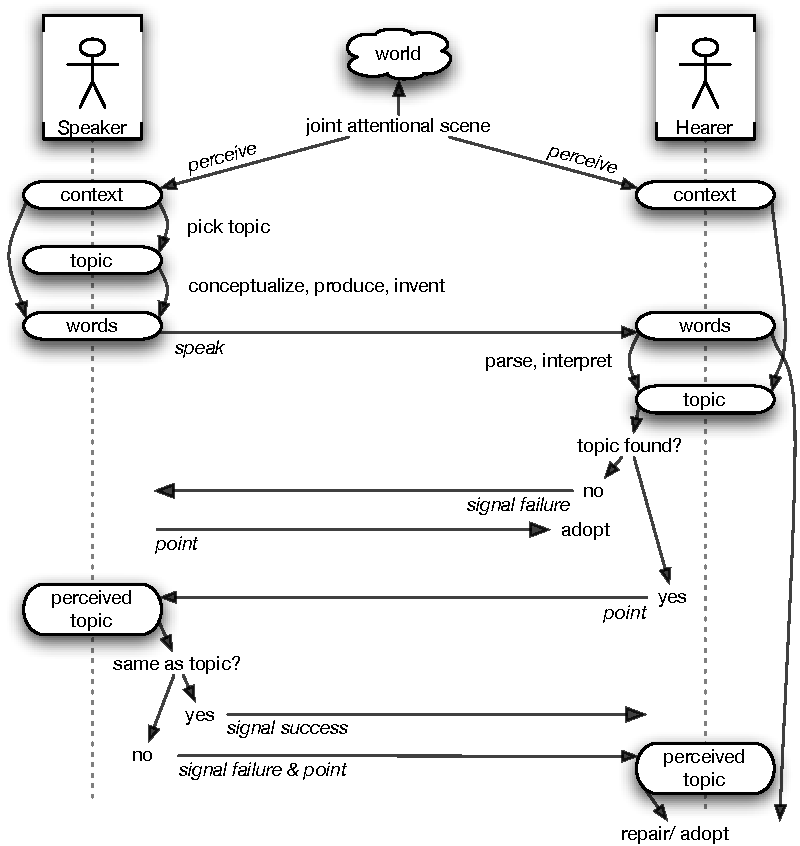
\includegraphics[width=0.80\textwidth]{figures/guessing-game-flow}}
  \caption{Flow of one language game. A speaker and a hearer follow a
    routinized script. The speaker tries to draw the attention of the
    hearer to a physical object in their shared environment.  Both
    agents are able to monitor whether they reached communicative
    success and thus learn from the interaction by pointing to the
    topic of the conversation and giving non-linguistic feedback.
    Populations of agents gradually reach consensus about the meanings
    of words by taking turns being speaker and hearer over thousands
    of such games. }
  \label{f:guessing-game-flow}
\end{figure}


Figure \ref{f:guessing-game-flow} shows a schematic view of the
language game that our agents are going to play (we will discuss each
of mechanisms mentioned below in much more detail in the description
of the actual experiments -- here we only will outline the general
dialogue script that is shared by all experiments throughout this
thesis). Two agents are randomly drawn from the population and
together establish a \emph{joint attentional scene}
\citep{tomasello95jointattention} -- a situation in which both agents
attend to the same set of objects in the environment and in which both
agents know that the respective other agent is attending to the same
set of objects. Once such a state is reached, the game starts. One of
the agents is randomly assigned to take the role of the speaker and
the other the role of the hearer. Both agents perceive then a
\emph{sensory context} from the joint attentional scene and keep it in
their short-term memory (visual perception and joint attention with
real robots is enormously difficult and we will dedicate the whole
Chapter \ref{c:embodiment} to that; in our experiments involving
simulated environments all these issues will be scaffolded and both
agents will perceive the same scene description that is generated by
the world generator mentioned above).

Next, the speaker randomly picks one object from his context to be the
\emph{topic} of the interaction -- his communicative goal will be to
draw the attention of the hearer to that object. For this he
constructs an utterance, which involves first coming up with a mental
representation of the meanings to express (\emph{conceptualization})
and then finding words that cover these meanings. When the speaker
does not have the necessary categories or words in his inventories, he
\emph{invents} them. Additionally, the speaker uses himself as a model
of the hearer and by listening to himself (\emph{re-entrance}), he
checks whether the words he came up with are clear and precise enough
to be understood (given his own inventories). Once the speaker is
satisfied with the constructed utterance, he speaks out the words to
the hearer. The hearer then \emph{parses} the utterance and tries to
find the object from his own perception of the scene that he believes
to be most probable given his interpreted meanings. He will point then
to that object and the speaker will either confirm that this was
indeed the object he intended to talk about (and signal
\emph{communicative success}) or he will point to his chosen topic
(and thus signal \emph{communicative failure}). It could also happen
that the hearer is confronted with a novel word or that his
interpretation doesn't match any of the objects in his context. In
this case, the hearer signals a communicative failure and the speaker
then also points to the object he intended. In both cases, the hearer
is able to learn from the interaction by \emph{adopting} the words
heard and associating them with the topic pointed at by the speaker
(and, if necessary, also inventing categories that are needed to
conceptualize the topic). Finally, at the end of each interaction both
agents \emph{adapt} their inventories based on the sensory context,
the topic, the words used and the outcome of the game in order to be
more successful in future interactions (\emph{alignment}).  The
population of agents plays \emph{series} of such language games. Each
agent starts with initially empty inventories and has never before
seen any of the objects in the world. Each agent tries to optimize his
own communicative success and cognitive effort and thus coherent
mental representations and shared language emerge (solely through
processes of invention, adoption and alignment) as a side-effect of
the game.

Finally some terminology issues: this type of game has often been
called \emph{Guessing Game}, either because the hearer has to guess
the topic of the utterance and point to it or because the hearer can
not know what aspect of an object the speaker intended with a
particular word (referential uncertainty, see below). When the focus
is on the kind of languages learnt, our game could be also called
\emph{Object Naming Game} because it is about naming objects (in
contrast to describing objects and their relations to other objects or
their roles in events). We will avoid possible confusions by always
using the term ``language game'' when referring to this particular
interaction pattern.


\subsection{Other social learning scenarios}

The language game paradigm has proved to be very successful in
demonstrating how groups of artificial agents can establish a shared
set of conventions through self-organization processes. However, when
it comes to explaining human communication, it has been -- rightfully
-- criticized for two reasons: First, it happens very rarely that
humans have to construct a communication system from scratch and the
normal case is that children learn the existing language of their
parents' culture. And second, the explicit feedback that our agents
give each other (including pointing and correnctions) is not necessary
for children to learn the
meanings of words.\\

\noindent Because our agents start without any prior language, speakers have to
invent words whenever their lexicons are not sufficient for their
communicative needs. And when multiple speakers independently invent
words for the same thing, a large number of competing words are
spreading in the population, before eventually one word ``wins'' and a
convention is established (as we will see further below). Although
some psychologists have demonstrated that humans are indeed able to
bootstrap and align symbolic communication systems in similar ways
(e.g. \citealp{galantucci05experimental,healey07graphical}), it is not
the normal situation that children are confronted with in language
acquisition -- they are born into a culture with an established
language and parents also won't adopt inventions made by their
children.

An alternative to this \emph{horizontal transmission} of language is
the \emph{iterated learning model}
(\citealp*{kirby01spontaneous,smith03iterated}; see also
\citealp{steels02iterated} for a comparison with the language game
framework). Instead of focusing on how language propagates within
members of the same generation, it investigates \emph{vertical
  transmission} from one generation to the next. Following an
inductive machine learning approach, training sets consisting of
meaning-form pairs created from a parent are used to train the
inventories of a child, which then becomes the parent for the next
generation. The language of the first generation is usually
initialized randomly.

However, the purely inductive nature of iterated learning leaves out
crucial aspects of communication such as joint attention, shared
context and communicative goals. Furthermore, languages also change
within generations and these changes can't be explained with effects
of vertical transmission because they rely on processes of
coordination and alignment.\\


\noindent The agents in our language game experiments always give each other
non-linguistic corrective feedback, i.e. the speaker either confirms
that the topic pointed at by the hearer was the intended one or he
points to the right topic. But children don't necessarily need such
social scaffolds in order to learn the language of their parents --
they are smart enough to make sense of the communicative intentions of
speakers, even when just overhearing conversations of others.
\cite{lieven94crosslinguistic} extensively reviews cross-cultural
differences in the social interactions from that children learn
language and the conclusion is that parents in some cultures give
extensive feedback, others almost not: ``children are clearly not
having to learn language from something like a television set; but nor
are they being presented with a graded set of syntax lessons''
\citep[p. 73]{lieven94crosslinguistic}.

Some researchers investigated other types of games with less explicit
feedback. Best known are \emph{Description Games} in which the speaker
describes a scene and the hearer either agrees that it is a good
description for the current scene or he disagrees. The disadvantage is
that the speaker has no way to verify whether the hearer indeed
understood him (the fact that the hearer agreed does not mean that
they had a similar understanding of the words used). But description
games actually need to be played when the topic of a conversation is
not an object (which can be pointed at) but for example an aspect of
an event or other relations between objects (which can't be pointed
at). The lacking consensus between speaker and hearer on what the
topic of the conversation is makes self-organizing a shared language
harder and the problem is usually tackled with
\emph{cross-situational} learning techniques (discussed further
below). \cite{vogt03investigating} have compared the performance of the
language game introduced above with so-called ``selfish games'', in
which there is no feedback at all (so it's like learning language from
a television set). Their conclusion is that selfish games are -- albeit
viable -- much more difficult.

Even if children don't need extensive teaching and feedback, it
nevertheless helps them. For example \cite{chouinard03adult}
demonstrated that learning improves when parents reformulate erroneous
utterances of their children. And \citet{tomasello83joint-attention}
compared lexical learning rates in trials where mothers directed the
attention of their children at novel objects with trials where they
just followed into what their child was looking at -- the results
suggest that joint attention supports lexical acquisition.
\cite{bloom01precis} puts it this way: ``The natural conclusion here
is that these naming patterns on the part of adults really are useful,
they just aren't necessary. Environments differ in how supportive they
are, and word learning is easier when speakers make the effort to
clarify their intent and exclude alternative interpretations. But
children are good enough at word learning that they can succeed
without such support '' (p. 1099).

Our agents don't have a `theory of mind', i.e. hearers have no
non-linguistic pragmatic means available to them for figuring out what
the speaker intends. And they don't have additional heuristics for
determining whether they reached their communicative goal, because
they use language only to direct attention (it would be for example
easier when the speaker would not try to draw attention to an object
but try to request the hearer to bring him the object -- if the hearer
brings another one then he knows that he said something wrong). The
only way for our agents to deal with these limitations is thus is to
establish joint attention and to use pointing as a means to check
whether the words were used correctly. So our language game is, in a
way, designed to overcome our agents' lack of social intelligence by
making it easy to verify whether communicative goals were reached. And
again \cite{bloom01precis}: ``Because of this, the best way to teach a
child an object name is to make it as clear as possible that you are
intending to refer to the referent of that name; and the best way to
do this is to point and say the word. In this way, the child can infer
that the speaker means to pick out the dog when using this new word,
`dog', and the meaning will be quickly and accurately learned''
(p. 1099).


\subsection{Evaluating the performance of language games}
\label{s:evaluating-language-games}

How can we then compare the performance of the different language game
experiments that we're going to do, i.e. how do we assess the
development of our agents' \emph{communicative competence}?
Intuitively, we would say that a person who knows more words than
somebody else and who complies better with the rules of for example
English is a better speaker of the language. The underlying conception
is that a language is some homogeneous public entity, casted into
dictionaries and internalized by its speakers. But even a person who
learnt the English dictionary by heart and follows all rules of the
language can still find himself in a situation where he will not
understand what other English speakers say. The person could for
example attend a mathematics conference and (although he understands
all the words) have no clue what they are talking about. Or he could
meet a group of adolescents who use slang words that did not make it
into the dictionaries yet.

Despite still ongoing debates about the historical distinction between
linguistic \emph{competence} and \emph{performance}
\citep{chomsky65aspects}, most linguists and philosophers agree now
that mastering a language is not about knowing the words and rules,
but about reaching communicative goals: ``We forget that there is no
such thing as a language apart from the sounds and marks people make,
and the habits and expectations that go with them. `Sharing a
language' with someone else consists in understanding what they say,
and talking pretty much the same way they do''
\citep[p. 131]{davidson05truth}. 

Therefore, we will make make \emph{communicative
  success} our main criterion for performance in language games. That
is, the focus is not on the content our agents' inventories, but how
they use this knowledge in communication. As detailed before (Section
\ref{s:language-game}), our language game script allows both the
speaker and the hearer to determine whether the communicative goal
(drawing attention to an external object) was reached. After each
interaction in an experiment's ongoing series of dialogues, we will
determine how the agents assessed their success in communication and
record it using the following measure:

\begin{measure}[h]{Communicative success}{m:communicative-success}
  Measures the fraction of successful games as assessed by the agents.
  An interaction is a success when the hearer is able to point to the
  topic intended by the speaker (see Figure
  \ref{f:guessing-game-flow}, page
  \pageref{f:guessing-game-flow}). After each successful interaction
  the value of 1 is recorded, for each failure 0. Values are averaged
  over the last n interactions (n=250 if not stated otherwise).
\end{measure}

\startfiguregroup
\begin{figure}[p]
  \gnuplotfigure{figures/communicative-success-example-average-window-1}
  \caption{Example for the evolution of communicative success over
    time. Values were recorded for 10 different series of the same
    experiment, each consisting of 10000 interactions. The size of the
    average window for recording the values of each series is 1,
    i.e. values within a series are not averaged.}
  \label{f:communicative-success-example-average-window-1}
\end{figure}

\begin{figure}[p]
  \gnuplotfigure{figures/communicative-success-example-average-window-100}
  \caption{A graph of communicative success in the same experimental
    run as above, but with values averaged over the last 100
    interactions in each series. Error bars are standard deviations
    across the 10 repeated series of the same experiment.}
  \label{f:communicative-success-example-average-window-100}
\end{figure}

\begin{figure}[p]
  \gnuplotfigure{figures/communicative-success-example-average-window-1000}
  \caption{The same as above, but with an average window of 1000. Note
    that this curve seems to be ``delayed'' compared to the other two
    as a result of the bigger averaging window. Another side-effect of
    averaging is the little ``bend'' in the curve at around
    interaction 1000.}
  \label{f:communicative-success-example-average-window-1000}
\end{figure}
\stopfiguregroup

\noindent Throughout this thesis, we will record such data along
repeated series of language tames (together with data of many other
measures) to generate graphs such as in Figures
\ref{f:communicative-success-example-average-window-1}--\ref{f:communicative-success-example-average-window-1000}. How
to read then these graphs? The recorded values (in this case for the
communicative success measure) are plotted over the number of
interactions along the x-axis. So in this example the agents reach an
average communicative success of about 80\% after 1000 interactions,
which then later on increases to about 95\%.

Three things are important when interpreting such graphs. First, the
fact that it takes 1000 interactions to reach 80\% success does not
mean that each agent played 1000 games up to that point. In the
example the population consisted of 10 agents, and with each time two
agents participating in an interaction, 1000 interactions means that
each agent played 200 games on average, being speaker in about 100
interactions. Second, values are averaged over an average window. The
example graphs show the same results for average windows of 1, 100 and
1000. Many authors in the field of artificial language evolution
include graphs such as Figure
\ref{f:communicative-success-example-average-window-1} in their papers
(no averaging). But we believe that the noisy curve in that example
does not add any information and makes comparisons with other graphs
harder. We will thus use higher averaging windows (usually 250, but
sometimes even higher), which produce cleaner curves. The disadvantage
of heavy averaging is, as it is shown in the other two graphs (Figure
\ref{f:communicative-success-example-average-window-100} and
\ref{f:communicative-success-example-average-window-1000}), that the
curves are a bit ``behind'' the non-averaged data (so this has to be
kept in mind). And, finally, third, we will always repeat the same
experiment 10 times and average the results of each series to rule out
effects of randomness (the agents will always talk about different
scenes, each time with other randomly chosen partners, leading always
to varying dynamics). The error bars in Figures
\ref{f:communicative-success-example-average-window-100} and
\ref{f:communicative-success-example-average-window-1000} still give a
hint on how values vary across the different series (they indicate the
standard deviation of the values at that interaction number in all 10
series).

Of course communicative success is not the only measure we are
interested in (we will introduce others later). Part of
self-organizing a language is also that agents improve their cognitive
economy. That means that inventory sizes will converge to an optimal
number of elements that are needed to cope with the communicative task
(making processing faster) and the number of changes in the agent's
inventories will decrease. And we will compute measures of
\emph{coherence} that indicate how similar the inventories of the
population's agents are. But, as we will see, it is possible (and in
the case of embodied agents unavoidable) that agents have very
different conceptual and linguistic inventories but still communicate
successfully. Thus: ``What matters, the point of language or speech or
whatever you want to call it, is communication, getting across to
someone else what you have in mind by means of words that they
interpret (understand) as you want them to''
\citep[p. 120]{davidson05truth}.



\section{Words: representing linguistic knowledge}
\label{s:representing-linguistic-knowlede}

\begin{figure}
  \parbox{0.6\textwidth}{\centerline{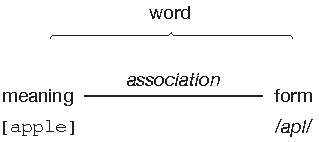
\includegraphics{figures/saussurean-sign}}}
  \caption{A diagram that illustrates our notion of the term ``word''
    as referring to the whole association of a meaning to a form.}
  \label{f:saussurean-sign}
\end{figure}

We have introduced the social context in which our communicative
interactions are going to take place. Next, we're going to define what
it means for our agents to ``know a language''. Since the focus of our
thesis is on lexicon formation (which leaves out many crucial aspects
of natural language such as grammar and morphology), our agents'
linguistic inventories are single \emph{lexicons}, consisting solely
of \emph{words}. Words are couplings between a \emph{meaning} and a
\emph{form} (see Figure \ref{f:saussurean-sign}) and we will
consistently use the term \emph{word} to refer to the whole of this
association (and not to the form). What meanings are and where they
come from will be the topic of the next Section \ref{s:meanings}. For
now we will treat them as sets of unstructured symbols (or
\emph{categories}, \emph{attributes}, \emph{features},
\emph{conceptual entities}, whatever you want to call them) such as
{\tt object-34}, {\tt category-17}, {\tt red-2} and so on. Forms are
random character strings that are created by speakers whenever they
invent a new word. Throughout our thesis, these forms will be built
from three random consonant/ vowel pairs such as for example in
``nuzega'' or ``firopa''.


\subsection{Saussurean signs}
\label{s:saussurean-signs}

For the coupling between meaning and form we rely on the concept of
the the \emph{Saussurean Sign} \citep{saussure67cours}. It is a
bi-directional relation between a concept (in the sense of some entity
of thought, \emph{signified}) and a form (a sound, a gesture, etc.,
\emph{signifier}). Bi-directional means that the same representation
is used to parse and produce utterances (which is not self-evident --
it is easy to imagine non-reciprocal communication systems in which
agents use different representations for parsing and producing or in
which agents lack the capability to either parse or produce). The
connection between the signified and the signifier is arbitrary, i.e.
there is nothing in the concept of a donkey that determines the sound
``donkey'' (in fact, different cultures arbitrarily connect very
different forms to similar concepts of donkeyness, e.g. ``Esel'' in
German). It's important to note that Saussurean Signs don't link
actual sounds waves to physical objects existing in the world but both
the signifier and the signified are mental patterns of reoccurring
sensory experiences of sounds and objects. Furthermore, and this will
be more clear later on, it is not the signs directly that determine
what we speak or how we interpret utterances -- it is the differences
in meaning and form between within a whole system of signs that govern
the speech of individuals (\emph{parole} in Saussure's terms). That
is, speakers don't follow explicit rules (in a classical artificial
intelligence rule system sense) such as {\tt \ "if donkey visible
  $\rightarrow$ produce sound `donkey'"} -- instead, they consider
their whole system of signs and their differences in meaning to
eventually use the sign that \emph{distinguishes} the donkey from
the other objects in the scene.

We'll assume Saussurean signs to be an appropriate construct for the
representation of form-meaning couplings in our work (especially the
notion of bi-directionality, arbitrariness and the importance of
relative differences to other signs), and we think that this is not a
controversial choice. But there is still the question of where this
particular nature of words comes from. To investigate this,
\cite{hurford89biological} compared different strategies for lexicon
formation in computer simulations. Learners either separately imitated
the production and speaking behavior of others or used observed
speaking behavior both in production and interpretation. The latter
strategy clearly had advantages because it makes it easier for the
agents to learn. Additionally, \cite{oliphant96dilemma} carried out
similar simulation studies which demonstrated that Saussurean
communication is favourable in populations of repeatedly interacting
agents (e.g. as in our language games), especially when the
populations are spatially organized. These experiments clearly show
that the Saussurean nature of words has advantages over other
communication systems. But the authors discuss these results under the
assumption that Saussurean communication evolved by means of natural
selection, a view that is challenged nowadays (see
\citealp[pp. 74--78]{bloom00how-children} for a discussion). As an
alternative, the bi-directional use of signs can be seen as a
consequence of our theory of mind: ``Children's ability to reproduce
intentional communicative actions via some form of cultural or
imitative learning involves a role reversal -- the child has
intentions towards the other person's intentional states -- which
leads to the creation of linguistic conventions''
\citep[p. 153]{tomasello01perceiving}. So we don't directly imitate
the linguistic behavior of others, that is, we don't imitate the
production of the sound ``donkey'' in the presence of a donkey but we
imitate the action of saying ``donkey'' as a method for directing
attention to donkeys. ``Once a child believes that the adult's use of
the word \emph{dog} was used with the intent to refer to a dog, then
she could use the same means (saying `dog') to satisfy this goal''
\citep[p. 76]{bloom00how-children}.

Finally, how are we going to implement our agents' systems of
Saussurean signs in terms of data structures? We'll choose the most
simple representation possible: a lexicon is represented as a list of
words, each having a meaning, a form and a score reflecting how
successful that word was used in past interactions. As we will see
later, the lexicon is usually part of a larger \emph{semiotic
  network}, a complex network \citep{strogatz01exploring} that
connects an agent's sensory experiences to forms and back and whose
overall behavior is the result of a coupling of different processes
that each have their own dynamics. There are many representations
thinkable that are more cognitively plausible than lists of words. For
example \cite{kosko88bidirectional} implemented a two-layer neural
network that can store paired data associations and
\cite*{billard99drama} developed DRAMA (dynamical recurrent
associative memory architecture) specifically for representing words
in robots. We prefer our representation over more integrated solutions
because it gives us full control over processes of language use and
learning. We assume that these structures could be easily transferred
into more natural representations (e.g. neural networks).


\subsection{Increasing complexity in the coupling between form and
  meaning}
\label{s:nature-of-form-meaning-couplings}


Words are couplings between meaning and form. We'll treat forms as
simple random strings and what meanings are will be explained in the
next section. We will turn now to the nature of this coupling, i.e.
how a form is coupled to meaning and how words in a lexicon relate to
each other. This structure is part of an agents cognitive
infrastructure, especially his mechanisms for production/
interpretation, learning and alignment. And it has direct consequences
on the dynamics of the language game experiments, i.e. how quick the
agents reach communicative success and coherence. Depending on the
``degrees of freedom'' in what the agents can associate to a form, in
how words with equivalent meanings/forms relate to each other, and in
how agents combine different words into utterances, various kinds (and
degrees) of \emph{ambiguities} arise in an agent's lexicon. For
example in all of these models it happens that different forms for the
same meaning spread in the population (because agents independently
invent them), causing \emph{synonyms} (the same meaning is associated
to multiple forms) to occur in the agent's lexicon. Similarly,
different contexts and other reasons might cause an agent to adopt
multiple meanings to the same form (\emph{homonymy}).

What does it mean for an agent to have for example a synonym in his
lexicon? Technically, an agent that learnt two different forms $f_1$
and $f_2$ for the meaning $m_1$ will not store them in the same word
with connections to both forms, but he maintains two separate
representations $w_1: m_1 \Leftrightarrow f_1$ and $w_2: m_1
\Leftrightarrow f_2$. Part of the self-organization process in the
series of language games is that the whole population eventually
agrees on one single form for a particular meaning (and vice
versa). In order to reach this goal, each agent individually tries to
optimize his own lexicon by preferring the most conventionalized
associations and eliminating \emph{competing} synonymous and
homonymous words. We will introduce various algorithms that achieve
this -- all of them rely on scoring each word depending on how
successful it is used in communication. When enough agents in the
population start preferring a particular form-meaning association, it
will prevail over the others, causing each individual agent to remove
competing synonyms and homonyms.

\begin{figure}[t]
\centerline{
\begin{tabular}{lp{1cm}l}
 A & & B \\
 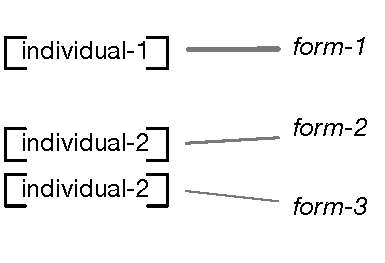
\includegraphics[width=0.30\columnwidth]{figures/models-of-form-meaning-couplings-1} & &
 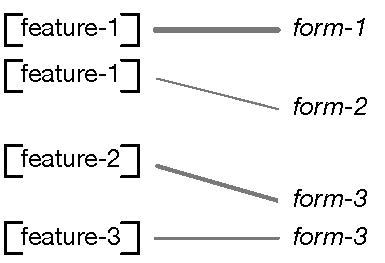
\includegraphics[width=0.30\columnwidth]{figures/models-of-form-meaning-couplings-2} \\
 & & \\
 C & & D \\
 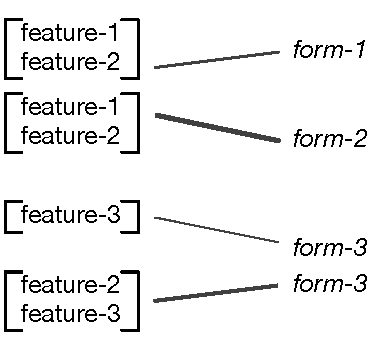
\includegraphics[width=0.30\columnwidth]{figures/models-of-form-meaning-couplings-3} & &
 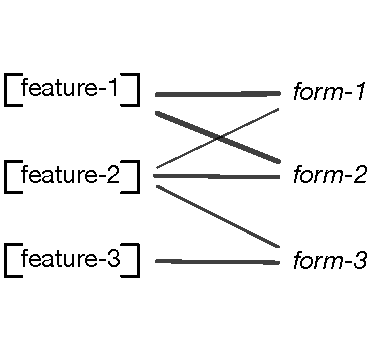
\includegraphics[width=0.30\columnwidth]{figures/models-of-form-meaning-couplings-4} 
\end{tabular}}
\caption{Increasing complexity in the nature of the coupling between
  form and meaning.  Hypothetical example lexicons of one agent are
  shown for four different models of lexicon formation.  Line widths
  denote different connection weights (scores).  A: One-to-one
  mappings between names and individuals in the Naming Game. There can
  be competing mappings involving the same individual (synonyms). B:
  One-to-one mappings between words and single categories in Guessing
  Games. Additionally to synonymy, there can be competing mappings
  involving the same words (homonymy). c: Many-to-one mappings between
  sets of categories and words. In addition to synonymy and homonymy,
  words can be mapped to different competing sets of categories that
  partially overlap each other. D: Flexible word meaning
  representations. Competition is not explicitly represented but words
  have flexible associations to different categories that are shaped
  through language use.
}
\label{f:models-of-form-meaning-couplings}
\end{figure}

Furthermore, other ambiguities arise from the use of \emph{multi-word}
utterances (it can become unclear which word covers which meaning),
from \emph{specificity} relations (whether a new word refers to the
whole object, to it's kind or a general property of it), and others.
The degrees of freedom in what to associate to a new form can be
interpreted as the \emph{complexity} of a lexicon formation model and
we will classify a variety of models according this degree of
freedom. For now, Figure \ref{f:models-of-form-meaning-couplings}
illustrates the nature of the coupling between meaning and form for
four of them.

The simplest of these four models, the \emph{Naming Game}
(\citealp{steels95selforganizing,steels99spatially}; Figure
\ref{f:models-of-form-meaning-couplings}A), is historically also the
oldest. The task in this game is to agree on a set of names for
established individuals (for example proper names such as ``John'' and
``Mary'' for individual persons).  Agents jointly perceive sets of
uniquely identifiable objects such as for example {\tt object-3}, {\tt
  object-8}, {\tt object-4}; or (as in
\citealp{steels95selforganizing}) unambiguously interpretable
positions on a spatial grid relative to the speaker (e.g. {\tt front},
{\tt side}, {\tt behind}, {\tt left}, etc). Words are thus one-to-one
associations between a representation for an individual and a name.
Since both speaker and hearer have the same representations of
individuals (the world they perceive consists already of
pre-conceptualized symbolic representations for unique objects or
locations), the hearer immediately knows which concept to associate to
a novel word after the speaker pointed to it. But synonymy can occur
because different speakers might invent different names for the same
object (for example in Figure
\ref{f:models-of-form-meaning-couplings}A the words {\tt
  individual-2}$\Leftrightarrow$\emph{form-2} and {\tt
  individual-2}$\Leftrightarrow$\emph{form-3} are synonymous).


Figure \ref{f:models-of-form-meaning-couplings}B illustrates a next
class of models. It is commonly referred to as a \emph{Guessing Game}
and was first introduced by \cite{steels96emergent}. It takes away the
scaffold that objects are represented as unique concepts by letting
the agents perceive scenes in which objects are sets of
pre-conceptualized discrete categories as for example in:
\begin{verbatim}
object-1: [weight heavy] [size medium] [shape square]
object-2: [weight light] [size small] [shape round]
object-3: [weight heavy] [size tall] [shape square]
\end{verbatim}
\noindent The speaker then searches for a category that
\emph{discriminates} the chosen topic from the other objects in the
context (for example {\tt [size medium]} discriminates {\tt object-1}
from the rest, {\tt [weight light]} or {\tt [shape round]}
discriminate {\tt object-2}, etc.) and then uses a single word to
express that meaning (the game stops when no discriminative category
can be found). So the words acquired by the agents are comparable to
adjectives for basic categories such as ``red'', ``small'' or
``round''. The representation of words is identical to those of Naming
Games (a one-to-one mapping between an atomic category and a form), but
further difficulties arise because the hearer does not know which
sensory quality (or channel) a novel word refers to. Consequently,
homonyms may appear in addition to synonyms because a hearer might
adopt different interpretations of the same word (for example in the
agent in Figure \ref{f:models-of-form-meaning-couplings}B interprets
the form \emph{form-3} both as {\tt feature-2} and as {\tt
  feature-3}). Because the words in this game still ``name'' single
categories, such experiments are sometimes called Naming Games as
well, reserving the term Guessing Game for the language game script.

\cite{looveren99multiple,looveren00analysis} presented two further
innovations: first, \emph{multi-word} utterances were introduced:
objects don't need to be discriminated anymore by a single category
but combinations of categories can be expressed by different words
(e.g. ``red'' and ``small'' when some other objects in the context are
also red and some others also small, but none of them red and small at
the same time). This leads to the additional difficulty that when a
hearer is confronted with two novel words at the same time then he
does not know which word covers which part of the inferred meaning
(such a situation is usually seen as too difficult: hearers only learn
when there is only one unknown word so that they can infer its meaning
using the know words and the context). Second, meanings of words can
be \emph{structured}: instead of expressing a single individual or
category, words are many-to-one mappings between forms and sets of
discrete categories (see Figure
\ref{f:models-of-form-meaning-couplings}C). Due to this, another
challenge arises for the hearer: he does not know to which subset of
the topic's feature he has to associate a new word. As a result, the
agents' lexicons do not only contain homonyms but also competing words
where the meaning of one is the subset of another (e.g. in Figure
\ref{f:models-of-form-meaning-couplings}C there are two words with the
form \emph{form-3}: one that expresses only {\tt feature-3} and one
that covers both {\tt feature-2} and {\tt feature-3}).


In order to scale up the above three lexicon formation models towards
more complex meaning spaces and in order to allow for the emergence of
more natural communication systems,
\cite*{wellens08flexible,wellens12multi-dimensional} proposed another
lexicon representation as shown in Figure
\ref{f:models-of-form-meaning-couplings}D. The main innovation is to
tackle ambiguities in what words mean with a \emph{flexible} coupling
between meaning and form: whereas agents in the previous models try to
figure out the meaning of a word by adopting multiple associations
between a form and its alternative meanings (and then use word scoring
techniques to rule out all of them except one), here the uncertainty
is put in the word representation itself. Instead of having a single
score for the whole coupling between a form and a set of categories,
each connection to a category is scored separately, which allows the
meaning of a word to gradually change towards its conventional use in
the population. Figure \ref{f:models-of-form-meaning-couplings}D tries
to illustrate this: an agent's lexicon is represented as a
many-to-many association between categories and forms, with each
connection scored separately.




\section{Meanings: grounded word semantics}
\label{s:meanings}

In addition to the social context of the communicative interactions
and the nature of word representations, the notion of ``meaning'' is
central to the understanding of communication in general and models
lexicon formation in particular. In our simulated language game
experiments, as discussed before, the world of the agents already
provides shared pre-conceptualized meanings consisting of (sets of)
symbols such as {\tt object-34}, {\tt category-17} or {\tt
  red-2}. With the meanings already being ``in the world'', they are
also immediately shared by all agents in the population and the
question what meanings are and where they come from is not posed --
the focus is rather on reaching consensus on which meanings to connect
to which forms. However, objects in the real world -- which is also
the world of our robots -- do not come with universally shared
properties directly accessible to observers. Instead, each agent has
to construct ``meanings'' as his own interpretation of a scene from
its sensori-motor interaction with the environment.



\subsection{From Saussure to Peirce}
\label{s:saussure-to-peirce}


A widely accepted notion of meaning is that they are not something to
be found in the world, but that they are used to \emph{refer} to
things in the world: ``The traditional view, emerging first in
Aristotle, is that the meaning of a word is what determines its
reference. ... Hence the meaning of \emph{dog} determines which things
are and are not dogs, and knowing the meaning of dog entails knowing
what things are dogs and are not dogs''
\citep[p. 18]{bloom00how-children}.

\begin{figure}
  \parbox{0.6\textwidth}{\centerline{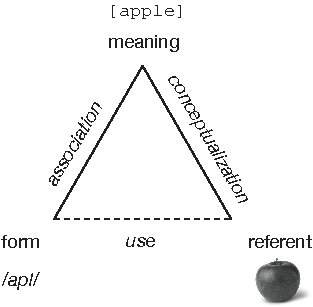
\includegraphics{figures/semiotic-triangle}}}
  \caption{Diagram of a semiotic triangle. The relation between a
    meaning, a form and a referent loosely resemble the definition of
    a sign by \cite{peirce31collected}. }
\label{f:semiotic-triangle}
\end{figure}


Adding referents to De Saussure's (\citeyear{saussure67cours}, see
also Section \ref{s:saussurean-signs} above) definition of a sign as a
relation between a meaning and a form, \cite{peirce31collected}
introduced the concept of a sign as a triadic relationship between a
form, a meaning and a referent (see Figure
\ref{f:semiotic-triangle}). Peirce originally used the term
\emph{representamen} for the \emph{shape} (form) of the sign and
\emph{interpretant} for its \emph{sense} or \emph{concept} (meaning).
For the referent, which is a physical object in the world but which
also can be abstract, Peirce used the term \emph{object}. 


The relation between form an meaning is, analogous to the Saussurean
sign, an arbitrary conventionalized bi-directional association between
a meaning and a form. And although finding the appropriate meaning
underlying a form or finding the form that expresses a meaning of
course requires some look-up process, these associations can be
considered to be ``stored'' in the lexicon of an agent. In contrast,
the relation between meanings and referents is of a different
nature. Word meanings are representations that allow to determine to
which referents a word applies and to which not. Therefore, finding
out whether a specific meaning is applicable to a specific referent in
the context is an active process that in each interaction again
establishes the relation between a meaning and a referent. We call the
process of determining the meanings that are applicable to a referent
\emph{conceptualization} and the reverse process of applying the
meanings underlying an utterance to a situation in order to determine
a referent \emph{interpretation}.


The third relation in Figure \ref{f:semiotic-triangle} between forms
and referents is even less direct. The meaning representations
maintained by each agent are not accessible by other agents -- they
can only observe forms and referents. Meanings thus constitute an
intermediate layer that allows agents to relate the same words to
similar referents in the world, i.e. \emph{use} a word in the same
way: ``For a large class of cases -- though not for all -- in which we
employ the word `meaning' it can be defined thus: the meaning of a
word is its use in the language'' \citep[Part I, Section
43]{wittgenstein67philosophische}. For example, the meaning of ``red''
is a shared convention how to classify the world into things that are
red and things that are not. Moreover, meaning representations are
constructed individually by each agent from sensory experiences of
specific referents. And because every agent has a different history of
interactions with the world and other agents, two agents will never
connect exactly the same meaning representation to the same
form. Intuitively, every two humans will also have slightly different
opinions about which border cases of red objects should be considered
red, but they will still use ``red'' successfully in most of the cases
to refer to red object. As we will see later, conceptual coherence,
i.e. the similarity between meanings acquired by different agents, is
not necessarily a prerequisite for successful communication. It is
enough that we all use a word to refer to the same things -- further
cognitive overlap is not necessary.


Furthermore, conceptualizing a referent or interpreting a meaning
never happens in a vacuum. Words can be used differently in different
contexts (for example ``the red block'' can be used to refer to an
orange block when all other objects are blue, but not when there is
another red block). And more importantly, the interpretation of words
depends also on the social context, i.e. the previous discourse and
the kind of communicative interaction. As discussed above in Section
\ref{s:language-game}, the language game played determines how words
have to be interpreted to yield a referent. ``We must therefore
explicitly acknowledge the theoretical point that linguistic reference
is a \emph{social} act in which one person attempts to get another
person to focus her attention on something in the world''
\citep[p. 97]{tomasello99cultural}. In our experiments, the type of
communicative interaction is fixed (see Figure
\ref{f:guessing-game-flow}, page \pageref{f:guessing-game-flow}) and
the implicit communicative goal underlying each utterance is to draw
attention to a single object in the environment of the
robots. Consequently, when an agent says for example ``red small'',
then the built-in convention is to interpret these words as ``please
point to the object that is small and red''.


The question of how to represent and process word meanings is very
closely related to the \emph{symbol grounding problem}
\citep{harnad90symbolgrounding}, which his ``... , generally speaking,
the problem of how to causally connect an artificial agent with its
environment such that the agent's behavior, as well as the mechanisms,
representations, etc. underlying it, can be intrinsic and meaningful
to itself, rather than dependent on an external designer or observer''
\citep[p.~177]{ziemke99rethinking}. The debate around this problem was
started by \cite{searle80minds} with the Chinese room argument as a
critique to early paradigms in artificial intelligence that envisioned
the possibility of intelligence based solely on the manipulation of
idealized \emph{physical symbol systems}
\citep{newell76computer,newell80physical} and since that has occupied
many philosophers and cognitive scientists. However, when adopting the
notion of meaning discussed above as a functional relation between
forms, internal representations and referents, then ``... one may
argue that argue that the semiotic symbol is \emph{per definition}
grounded, becasue the triadic relation (i.e. the semiotic symbol)
already bears symbols meaning with respect to reality''
\citep[p.~434]{vogt02physical}. We will thus not take part in this
debate and rather focus on the technical challenge of the acquisition
of meanings through the interaction of a physical body with the
environment and on processes for conceptualization and semantic
interpretation, which together ``solve the symbol grounding problem''
\citealp*{steels08symbol-grounding,steels07semiotic}.



\subsection{Mental representations for categorization}
\label{s:mental-representations-for-categorizations}

Peirce's definition of a sign can be discussed without subscribing to
any theory of what word meanings are and how they are represented in
an agent, a question which has occupied philosophers, logicians,
linguists and psychologists for a very long time. We will not delve
into the history of this debate but rather stick with contemporary
notions of meaning in the cognitive sciences that are based on the
concept of \emph{categories}, as advanced by scholars such as
\cite{lakoff87woman}, \cite{harnad87categorial} or
\cite{barsalou99perceptual}. A category is a representation that
allows to classify objects according to some criterion or ``a category
exists whenever two or more distinguishable objects or events are
treated equivalently'' \citep[p. 89]{mervis81categorization}. We call
the long-term memory of categories that are acquired by an agent an
\emph{ontology}.


Categories are abstractions from the continuous sensori-motor
interaction with the environment that have proved to be useful for an
agent, for example in communication: ``one purpose of categorization
is to reduce the infinite differences among stimuli to behaviorally
and cognitively usable proportions. It is to the organism's advantage
not to differentiate one stimulus from others when that
differentiation is irrelevant for the purposes at hand'' \citep[page
384]{rosch76basic}. Consequently, well-tuned category systems
contribute to the cognitive economy of an agent because they limit the
number of sensori-motor patterns that have to memorized and they can
be processed independently of the context in which they were created
and the objects and the events that they stand for, a phenomenon which
\cite{gardenfors05detachment} calls the ``detachment of
thought''. Finally, categories are not only used for language, but
also for a big variety of other cognitive activities such as for
example planning. Some scholars such as
Peirce~(\citeyear[p.~2.302]{peirce31collected}) even claim that ``we
think only in signs''.


Early psychological studies by \cite{rosch73natural} have shown that
many categories do not have strict borders but that membership to a
category is continuous. For example, the category \texttt{red} does
not unambiguously divide all things in the world into a set of objects
that are red and into another set of objects that are not red, but
instead provides a graded judgement of \emph{how} red an object
is. And at least for `basic level' categories, \cite{rosch73natural}
demonstrated that the gradedness of this classification is a function
of the similarity to a \emph{prototype}, which can be understood as a
point in a sensori-motor space that defines the center of the
category. Such a space is defined by multiple dimensions representing
continuous sensory or other qualities and multiple categories defined
by points in that space. For example color categories can be
represented as points in a two- or threedimensional color space and
color categorization of an object then means to find the category that
has the closest geometric distance to a stimulus. Along that line,
\cite{gardenfors00conceptual-spaces} introduced the theoretic
framework of `conceptual spaces' for an operationalized geometric
account of categorization and provided examples for many domains, such
as for example in \citep{gardenfors01reasoning}.\\


\noindent As mentioned before, we will not to equip our agents with pre-existing
engineered sets of categories but endow them with mechanisms for the
autonomous creation of truly grounded ontologies. For that, most work
on category formation in the field of artificial intelligence has been
done (very successfully) using techniques of machine learning
\citep{mitchell97machine}. Such learning methods always require data
sets of example stimuli together with their correct classification
(usually labelled manually by a human) and then a classifier (for
example based on a neural network or a K-nearest neighbor algorithm)
is trained so that it eventually can reproduce the classificaton that
is implicit in the example set. However, there are three problems with
such approaches: First, in open-ended interaction and learning
scenarios where the things to expect in the environment are not known
in advance, proper training sets may not be easily available at all.
Second, once classifiers are trained, they don't adapt and thus the
learnt classification may become inappropriate when new types of
objects occur in the environment (which is the case for humans and for
our robots). And third, the categories learnt with machine learning
techniques are still induced by a designer because he used his own
(human) category system to create the labelled data sets. For a
further discussion of the problems involved in applying machine
learning techniques to autonomous category formation, refer to
\citep{steels97constructing}.


We will thus need mechanism that allow our agents to gradually
construct and shape their ontologies from the continuous interaction
with the environment and other agents, in a similar way to the
self-organization of lexicons discussed above. One method for this
introduced by \cite{steels96perceptually} are \emph{discrimination
  trees} (we will disscuss them in Chapter
\ref{c:grounded-categories}). He presented simulated agents with
generated contexts consisting of objects characterized by real-valued
features and in order to be successful in discriminating one object
from the other objects in such a generated context, they created
categories by further and further sub-dividing the range of feature
values into smaller and smaller regions (hence the term discrimination
tree).  Discrimination trees were then implemented by
\cite{steels97constructing,steels97grounding} on wheeled LEGO robots
to create categories for distances measured with infrared sensors and
later by
\citep{steels99situated,steels99collective,steels02bootstrapping} in
the Talking Heads experiment (discussed further below) for visual
features such as color, size and position obtained by pan-tilt cameras
directed at a whiteboard with objects. Also with LEGO robots,
\cite{vogt01bootstrapping,vogt03anchoring} conducted similar
experiments, but instead of discrimination trees, categories were
created as prototypes in the sensory space of a bigger range of
distance sensors. Finally, the formation of color categories using
various prototype-based approaches was studied extensively by
\cite{steels05coordinating} who presented agents with perceptions of
sets of color chips and by \cite*{bleys09grounded} who used the same
robotic setup with humanoid robots as in this thesis.




\subsection{Categories and language}

Because the agents in our experiments will construct and shape their
ontologies exclusively for the purpose of being successful in the
given task of communicating about objects in their environment, both
the adequateness of each agent's individual category system as well as
the coherence between different agents' ontologies directly have an
impact on the overall communicative success of the population, which
in return means that success in communication is a also a good measure
for driving the self-organization of the category
systems. Consequently, effective mechanisms for orchestrating the
co-evolution of conceptual and linguistic inventories through a tight
coupling are crucial for successful communication (see
\citealp{steels98origins-ontologies} for a discussion and review of
early experiments).

\begin{figure}[t]
  \centerline{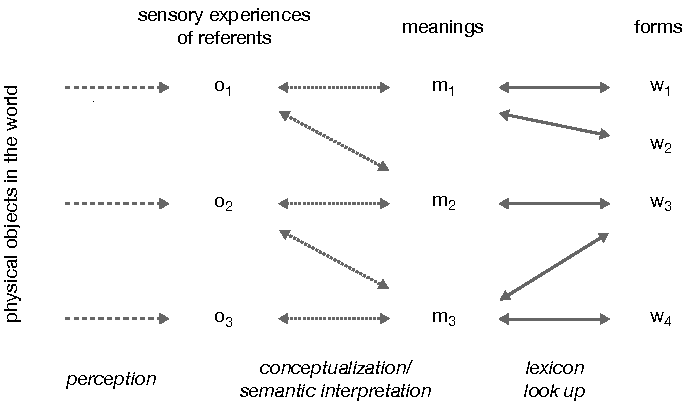
\includegraphics{figures/semiotic-network-example}}
  \caption{A schematic model of an agent's semiotic
    network. Perceptual processes yield representations of sensory
    experiences that then become connected to meaning representations
    through processes of conceptualization and semantic
    interpretation. Forms are connected to meanings through a lexicon
    look up process.}
  \label{f:semiotic-network-example}
\end{figure}


The perceptual, conceptual and linguistic representations that are
maintained by each agent for producing and parsing utterances can be
viewed as a \emph{semiotic network} as shown in Figure
\ref{f:semiotic-network-example}. Long-term memories of meanings are
connected to forms through persistent associations that are stored in
the agent's lexicon. For production and parsing, a look up process
retrieves the best form connected a meaning and vice versa. In
contrast, representations of sensory experiences that are created by
perceptual processes for referents are only memorized over the course
of a single interaction. They become dynamically connected to meanings
through processes of conceptualization and semantic
interpretation. Each of the connections between representations in a
semiotic network is weighted. Scores of form meaning associations
reflect how well a word was used in the past and conceptualizations
are scored based both on how well a category discriminates a referent
from the context and on success in previous interactions. Producing or
parsing an utterance then amounts to finding an optimal path through
the network, either by always following connection with highest weight
or by searching for the highest cumulative score.


The biggest challenge in maintaining semiotic networks lies the
coupling between the alignment dynamics of meanings and of words. The
communicative success perceived by an agent only provides an overall
measure for the appropriateness and degree of conventionalization of
all the representations along a particular path through the semiotic
network. For example when an interaction fails, an agent has no
guaranteed way of attributing the failure in order to repair its
network -- it could be both due to an inappropriate category, due to a
wrong word, or due to a disadvantageous connection weigth that
prevented the agent from using the `right' path through the network.
Similarly, also positive communicative feedback only acts on both the
involved categories and words and as we will see later on, it needs
many interactions to disentangle the fortune of particular categories
from those of the words connected to them.\\


\noindent By letting agents create and align meanings in a way so that
they fit well with the linguistic conventions in a population, we give
language a very prominent role in the formation of categories, which
is not an uncontroversial choice. Next to language that imposes and
structures concepts, there are at least two other important factors:
First, while it is very unlikely for most of the categories to be
innate, the genetic endowment of agents certainly constrains the
morphology of the body and its perceptual apparatus. And similar
sensori-motor interactions with the environment lead to a similar
structuring of reality. Second, the structure of the world itself also
constrains concept formation. Some patterns in the world occur more
often than others and some distinctions are more salient than others,
and for efficient communication it makes sense to reflect these
patterns in the language. How these three factors are weighted is an
ongoing debate in the cognitive sciences and we will not take a stance
in this discussion. In our experiments, language, the body and the
world play an equally important role.

Nevertheless, the previously unpopular theory of \emph{linguistic
  relativity} which proposes a strong influence of language on the
nature of categories (or Sapir-Whorf hypothesis,
\citealp{whorf56language}) started to receive more an more support
recently (see for example \citealp{levinson01language} for a review of
empirical evidence and arguments). And there is quite of number of
computational studies demonstrating that the shaping of categories
through language is beneficial for the self-organization of
communication systems. For example \citep{cangelosi02adaptive} showed
in an experiment where simulated agents were interacting in a
toy-world consisting of mushrooms (with some of them being poisonous)
that agents that have to construct their sensori-motor categories
solely by trial-and error interactions with the environment have an
evolutionary disadvantage compared to those whose categories are
shaped through language.


A related question is whether the learning of word meanings requires
the pre-existence of categories (learnt or innate) or whether, in the
other extreme, the mental world is exclusively structured through
language. In humans, linguistic development is preceded by a phase in
which mental representations are constructed solely from the
non-linguistic interaction with the world. However, concepts such as
number systems or as simple as color categories are clearly culturally
transmitted and thus even if language initially relies on pre-existing
representations, in later stages there is a co-evolution of categories
and words and we will also pursue that strategy in our experiments.
In support, \cite{clark04how} reviewed empirical evidence (for the
domain of space) on how children first build on conceptual
representations acquired in pre-linguistic stages and how these
representations are refined or build upon later when learning the
underlying representational structure of the parent's language.


Finally, the issue of planning and interpretating multi-word
utterances is also linked to the interplay between categories and
language. First of all, we need to define what the meaning of an
utterance is: in interpretation, it is the combined meanings of all
the words involved in parsing. Consequently, when an agent connects
many different meanigns to the same word forms, then many different
sets of categories can result from applying a lexicon. Semantic
interpretation of such a list of categories will then look for the
object that fits all categories best. In production, conceptualization
processes try to find a set of categories that disriminate the chosen
topic from the other objects in the context. Lexicon application then
needs to find a combination of words that \emph{cover} each of the
categories in the meaning, a process which again can yield multiple
combinations of words.

In general, agents trace their semiotic networks in parallel for the
involved representations and additional conceptualization and lexicon
processes need to check whether combined sets of categories and words
are applicable to a context, meaning or utterance. How exactly
linguistic and semantic representations are to be processed is
implicitely hidden in the language game and shared by all agents. For
advancing this work towards grammatical language, more explicit means
of representing how to apply categories are certainly needed and a
good candidate for this is the \emph{IRL} framework
\cite*{steels05planning,vandenbroeck08constraint-based,spranger10open-ended-semantics,spranger10open-ended,spranger12openended}
which enables agents to autonomously construct compositional semantic
structures that configure the interplay of cognitive categorization
operations and categories.






%%% Local Variables: 
%%% mode: latex
%%% TeX-master: "thesis"
%%% End: 

%% \setcounter{chapter}{2}

\chapter{Models of lexicon formation}
\label{c:thesis-overview}

In this thesis we will systematically analyze the performance of
different classes of lexicon formation models. Starting simple, we
will confront our agents with more and more challenging communicative
tasks and each time examine what additional representational
mechanisms and learning strategies are required to reach communicative
success and coherence. In doing so, we will follow the increasing
complexity of models that we laid out in Section
\ref{s:nature-of-form-meaning-couplings} (page
\pageref{s:nature-of-form-meaning-couplings}).

In order to be able to evaluate the impact of the additional
challenges stemming from embodiment and real-word perception, we will
first investigate lexicon formation in simulated worlds: throughout
Part \ref{p:II}, agents will be presented with idealized simulated
perceptions of varying complexity. To set the stage, we will briefly
review models for the naming of individual objects in Chapter
\ref{c:naming-game}.  From there on, we discuss strategies for dealing
with ambiguity that arises from conceptualization, multi-word
utterances and structured meanings in Chapter \ref{c:gg}. Motivated by
these results, we introduce a flexible model of word meaning
representation and learning in Chapter \ref{c:flexible}. 

Part \ref{p:III} then discusses embodied models of lexicon
formation. We will first introduce the robotic experimental setup with
its mechanisms for visual perception and social cognition in Chapter
\ref{c:embodiment}. Then we look at how robots can construct notions
of object individuality as a prerequisite for aligning sets of proper
names in Chapter \ref{c:gng}, and how more general categories can be
grounded trough language games in Chapter
\ref{c:grounded-categories}. Finally, in Chapter
\ref{c:flexible-grounded} we apply the model from Chapter
\ref{c:flexible} to real-word embodiment and
analyze its performance.\\



\section{Guessing the meaning of novel words}

Because there is no direct relationship between word forms and
referents and due to the nature of words as arbitrary relationships
between meanings and forms, hearers are faced with the challenge of
guessing the meaning of novel words. When the hearer does not know a
word (and can not infer its meaning using the other words in the
utterance and the context), then he non-linguistically signals a
communicative failure and the speaker will then point to the intended
referent. Although this pointing will unambiguously establish shared
reference, the hearer does not know which aspect of the referent is
covered by the unknown word: it could be its color, its size, or even
a combination thereof.

The degree of this uncertainty depends on the nature of the
coupling between meaning and form. When single word forms map to
single categories that stand for unique referents as a whole, then
there is no uncertainty for the hearer at all and he just needs to
associate a novel word to his conceptualization of the individual
object. But as soon as words refer to categories such as \texttt{red}
or \texttt{small}, hearers need to infer which category was meant upon
hearing a novel word. This problem gets multiplied when the language
game involves multi-word utterances (and when thus it is not clear
which word covers which part of the meaning) or when word meanings are
allowed to be structured (a word can refer to single categories or
combinations of categories, see Section
\ref{s:nature-of-form-meaning-couplings} on page
\pageref{s:nature-of-form-meaning-couplings}).


The challenge of dealing with this uncertainty is usually linked to
the problem of \emph{referential indeterminacy} and a thought
experiment carried out by \cite{quine60word}: he discussed an imagined
situation in which a field linguist tries to learn a language
unfamiliar to him from a native speaker. As they walk through a
forest, they encounter a rabbit and the native points to it and says
the word ``gavagai''. The linguist then forms the reasonable
hypothesis that the word means \texttt{rabbit}, but Quine makes point
that he can not be sure what the meaning of ``gavagai'' is and that
there is potentially an infinite number of possible meanings: it could
mean ``Let's go hunting'', ``There will be a storm tonight'', ``dinner'',
and so on.


Children also face the problem of referential uncertainty when
learning their mother tongue. Nevertheless, they learn words
extraordinarily quickly, from only a very few or even one
exposures. This phenomenon is called ``fast-mapping'' and was
extensively studied by \cite{carey78child}. Although it can take years
for children to home in to the proper meaning of words in all their
nuances, children make very good initial guesses about what words
refer to. In the literature, there is an enormous amount of empirical
studies showing that children prefer some interpretation of novel
words over others. For example \cite*{akhtar96role} showed that in a
object naming task with toy objects, 24-month-old children tend to
associate unknown words with objects that are novel in the
context. Similarly, \cite*{smith96naming} demonstrated that
three-year-old children rely on relative saliency when selecting
features for learning names for objects with attached parts.


Citing these findings, many researchers have concluded that children
thus must be endowed with (possibly innate) word learning
\emph{biases} or \emph{constraints} \citep{markman92constraints,
  gleitman90structural}. In this theory, constraints greatly reduce
the hypothesis space of possible meanings and only due to that make
the task of learning a language achievable. For example
\cite{macnamara82names} proposed the \emph{whole object bias}:
children assume that a novel label is likely to refer to the whole
object and not to its parts, substance, or other
properties. Furthermore, \cite*{landau98object} suggested the
\emph{shape bias} -- children initially use object shape as the main
categorization ground and only later on incorporate other properties
such as its function. And with the \emph{mutual exclusivity
  constraint} \citep{markman88childrens}, children assume category
terms are mutually exclusive, i.e. a novel word can not refer to a
property of an object for which the child already knows a
word. Similarly, \cite{clark87principle} formulated the
\emph{principle of contrast} (every two forms contrast in meanings)
and the \emph{principle of conventionality} (for each meaning, there
is a conventional form that speakers expect to be used in the language
community).\\


\noindent All these studies clearly show that children indeed consistently
prefer some interpretations of novel words over others and as we will
see, implicitly using some of these strategies such as the principle
of contrast or the mutual exclusivity constraint in our lexicon
formation experiments will also help to reach coherence in the
population. There is, however, a debate whether it is necessary to
assume language specific biases or constraints to explain these
empirical results or whether they can be the consequence of other,
possibly more general, cognitive mechanisms.


Most prominently, \cite{tomasello03constructing,tomasello99cultural}
argues that no special mechanisms are needed and that word learning to
a large extend relies on the children's general ability to understand
the intentions of their caregivers in naturally occurring social
interactions \citep{tomasello01perceiving} and in the motivation to
participate in joint activities and to share psychological states with
others \citep*{tomasello05understanding}. We share the stance that
``These findings are consistent with the view that fast mapping
emerges from a general capacity to learn socially transmitted
information -- including, but not limited to, the meanings of words''
\citep[p. 34ff]{bloom00how-children}.


Others have explained children's word learning skills with the ability
to observe statistics in co-occurrences between objects and words, a
theory called \emph{cross-situational learning}. For example
\cite{akhtar99early} presented children with novel objects that varied
in shape and texture. By consistently labelling objects of similar
properties ``a modi one'', children associated the quality that
remained constant across trials to the new word. In a more recent
study, \citep{smith07infants} showed similar effects for associating
novel words to more holistic concepts such as \texttt{ball} and
\texttt{dog}.


Inspired by this empirical evidence, scholars such as
\cite{siskind96cross-situational} and \cite*{smith06cross-situational}
operationalized their understanding of cross-situational learning in
computational studies on lexicon formation. In this technique, a
learner initially derives a set of possible \emph{candidate} meanings
from the context and stores all of them with a novel word. In
subsequent exposures to the same word in other contexts, the hearer
eliminates all those meanings that are not consistent with the context
(i.e in the intersection with the meanings derived from the current
context) until unambiguous mappings are found. There are, however, a
number of problems with this approach. Requiring observation of many
word - context pairs, the time to gain usable word meanings by far
exceeds the number of exposures that children need on average. Second,
in order to enumerate all possible meanings of a novel word and for
using the technique of intersecting meanings across contexts, the
learners need fully established category systems that do not change,
which is often not the case when for example robotic agents co-evolve
their ontologies with lexicons in the learning process. Consequently,
most computational experiments on cross-situational learning have been
done in simulated worlds where the environment already provides
pre-conceptualized atomic meanings that are shared between speaker and
hearer (with exceptions such as in
\citealp*{debeule06cross-situational}). Third and finally, models of
cross-situational learning usually consider single-word utterances and
unstructured word meanings. Scaling to more complex communicative
challenges as introduced in this thesis has proved to be difficult
\citep{vogt03investigating}.\\

\noindent In general, we find the notion of a \emph{hypothesis} space that gets
\emph{pruned} over the course of many interactions problematic. We
will show in this thesis that lexicon formation models that consider
word learning as an enumeration and subsequent elimination of
alternative hypotheses will not scale well with increasing population
sizes, meaning spaces, and the challenges of embodiment. Instead we
will argue for models in which learners construct and gradually shape
word meanings \citep{bowerman01shaping}. The hypothesis is that
``\dots the use of words in repeated discourse interactions in which
different perspectives are explicitly contrasted and shared, provide
the raw material out of which the children of all cultures construct
the flexible and multi-perspectival -- perhaps even dialogical --
cognitive representations that give human cognition much of its
awesome and unique power'' \citep[p. 163]{tomasello99cultural}.
Although in this view learners also make guesses at the meaning of
novel words, they are different in nature. Children cannot have at
hand all the concepts and perspectives that are embodied in the words
of the language they are learning -- they have to construct them over
time through language use. ``For example, many young children
overextend words such as \emph{dog} to cover all four-legged furry
animals. One way they home in on the adult extension of this word by
hearing many four-legged furry animals called by other names such as
\emph{horse} and \emph{cow}'' \citep[pp
73--74]{tomasello03constructing}.



\section{Scaling, robustness and the challenge of real-world
  perception}


The second focus of this thesis is on \emph{scaling} and
\emph{robustness} of lexicon formation models. We will investigate how
well models perform with increasing communicative challenges and by
that try to find the boundaries in which they are applicable. Many of
the models reviewed here only have been tried in ``easy enough''
environments and tasks and we will systematically analyze under which
conditions they fail and why. Most importantly, we will test all our
models with respect to how well they scale with larger population
sizes. Virtually every model in the literature works properly when the
number of agents in the population is two, because then each agent is
part of every interaction and conventions thus become easily
shared. But whereas many models scale well to small population sizes
of 5 to 10 agents, they often become impractical for populations of
100 or 1000 agents due to fundamental shortcomings in the way how
words and meanings are represented and processed. Similarly, scaling
with meaning spaces is an issue. We will evaluate population dynamics
in worlds with increasing number of objects and rising complexity and
structuredness of (simulated) perceptions.


On the other hand, we will argue that under the condition that some
crucial dynamics are in place, lexicon formation models are robust
with respect to the particular strategies chosen for invention,
adoption and alignment. For example, many algorithms have been
proposed for updating the inventories of agents after an interaction
based on the outcome of the game, and we will dissect which of them
are really required to reach success and coherence. \\


\noindent Related to scaling and robustness is the issue of the
influence of real-world perception on lexicon formation models. First
of all, not providing agents with shared symbolic perceptions adds the
additional complexity of category formation, which creates new kinds
of dynamics when ontologies and lexicons are constructed in parallel
and interdependently. For example, strategies for updating word
confidences also need to take into account that underlying categories
also may have shifted their meaning. Or when an interaction fails,
there is the hard decision to make whether the categories involved
were inappropriate or whether the word forms were simply not
conventionalized.
 
Furthermore, embodiment creates other kinds of uncertainties that need
to be dealt with. Agents can view a scene from different angles,
lighting conditions may vary and thus the perceptions that two
different robots have of the same physical object will never be the
same. Even a single robot will perceive an object differently over the
course of time due to camera noise, robot motion and general
uncertainty in computer vision systems. Nevertheless, human concepts,
such as, for example, the color red, are robust to such influences --
we will recognize an object as red under very different lighting
conditions and even subjects with color deficiencies are often able to
communicate about colors.

Concretely, embodied lexicon formation models need to cope with
\emph{perceptual deviation}, i.e. that specific continuous features
(e.g. position, shape, width and height, color information, etc.)
computed by the vision system for an object differ drastically between
the perception of speaker and hearer. For example one robot might
perceive the height of an object as being {\tt 0.72} and the other one
as {\tt 0.56}. This will inevitably cause each agent to have a
different notion of a word such as ``high''. We will make the point
that investigating lexicon formation with real robots leads to more
robust and realistic models, which in turn also perform better in
simulated environments.







%%% Local Variables: 
%%% mode: latex
%%% TeX-master: "phd-thesis"
%%% End: 



%% \part{Strategies for lexicon formation in simulated worlds}
%% 
\setcounter{chapter}{3}

\chapter{Establishing names for unique objects}
\label{c:naming-game}

To set the stage, we will now briefly introduce the lexicon formation
model that is commonly referred to as the ``Naming Game''. In such a
language game, agents learn to associate single word forms to atomic,
unstructured meanings which are provided by a shared simulated
environment. Whereas in the initial publication by
\cite{steels95selforganizing} the meanings were pre-conceptualized
spatial categories such as \texttt{left} and \texttt{front}, later on
(e.g. in \citealp{steels99spatially}) shared concepts for unique
individual objects such as \texttt{obj-4} and \texttt{obj-17} were
normally used. Since then, the Naming Game has become a general
vehicle for investigating the emergence and spread of conventions in a
population, where conventions not necessarily need to be form-meaning
associations but can be any trait that is negotiated in a population,
such as for example preferences or beliefs.\\

\noindent No other lexicon formation model has been as extensively
investigated as the Naming Game and we will not re-discuss all these
results. We will rather introduce it here as a baseline for all the
other experiments in this thesis and only focus on aspects that we
will also need later on. 


\section{Strategies for representing, processing and
  learning of words}
\label{s:ng-strategies}

In all experiments in this thesis, language users are modelled as
software agents following standard practices in the field of
Artificial Intelligence (see
e.g. \citealp{wooldridge95intelligent}). That is, each agent has its
own private state and autonomously responds to changes in the
environment and to actions of other agents. It is important that
agents do not have access to mental representations of other agents
(i.e. there is no telepathy). Instead, they are only able to observe
the actions of their interlocutors such as utterances, pointing,
non-linguistic feedback and so on.

\begin{figure}[t]
  \centerline{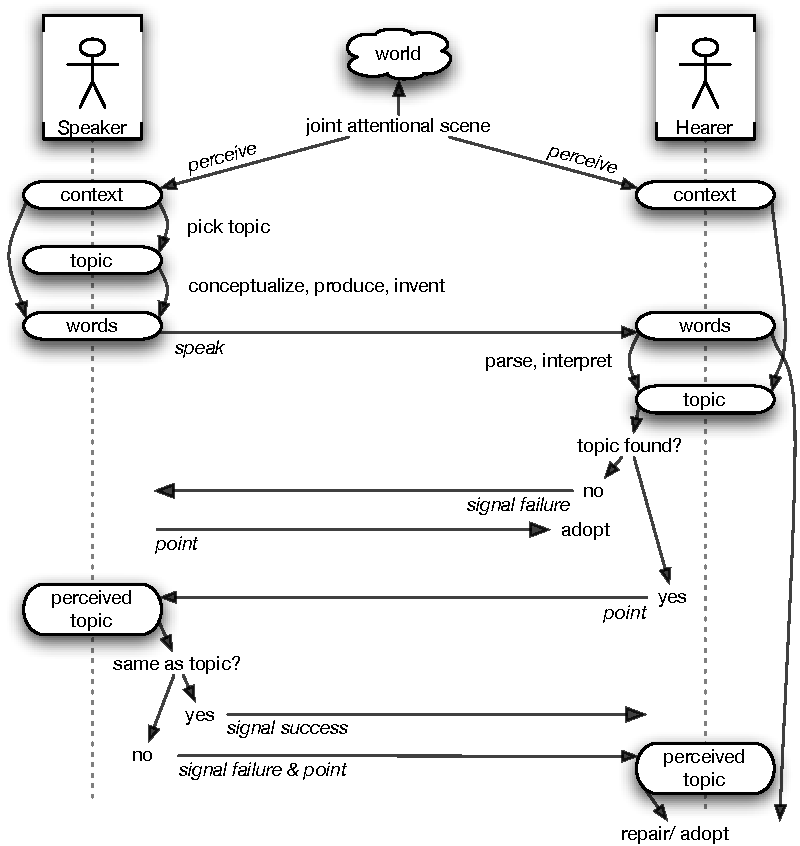
\includegraphics[width=0.80\textwidth]{figures/guessing-game-flow}}
  \caption{Main steps and mechanisms involved in a communicative
    interaction (see also Figure
    \ref{f:guessing-game-flow}).}
  \label{f:guessing-game-flow-2}
\end{figure}

At the begin of an experimental run, the population $P :=
\{a_1,a_2,\dots\}$ is created (we will by default use a population
size $|P| = 10$) and the agents $a_i \in P$ are initialized with empty
linguistic (and conceptual) inventories. Before each communicative
interaction, two agents are randomly drawn from this population and
assigned the communicative roles of speaker and hearer. To play a
language game, the speaker and hearer follow a built-in script that is
shown again in Figure \ref{f:guessing-game-flow-2} (see also Section
\ref{s:language-game}, page \pageref{s:language-game}). 

This particular type of language game will form the basis of all
experiments in this thesis and the particular lexicon formation models
will only differ in their strategies for representing, processing and
learning of lexicons and ontologies. We will now define these
mechanisms for the Naming Game and later on only discuss the
differences to this model:

\inparagraph{Lexicon representation} Each agent $a$ in the
population $P := \{a_1,a_2,\dots\}$ maintains a lexicon $L(a) :=
w_1(a),w_2(a),\dots$ consisting of a set of words $w(a)$. A word is
represented as a three tuple $w := \langle m(w), f(w), \gamma(w)
\rangle \in {\cal M}\times{\cal F}\times \mathbb{R}$, which is an
association of a meaning $m(w) \in {\cal M}$ to a form $f(w) \in {\cal
  F}$ with an association weight $\gamma(w)$ representing the agent's
confidence in that association. ${\cal M}$ is the set of possible word
meanings, ${\cal F}$ the set of possible word forms and $\gamma(w)$ a
real value with $0 \leq \gamma(w) \leq 1$.

\inparagraph{Perception} The world in which the agents interact
consists of shared atomic meanings $m \in {\cal M}$, which can be
anything but are typically seen as `individual objects'. In each
interaction both the speaker and hearer are provided with the vector
of all meanings in the world as their perception of the scene. By
default, the number of meanings in the world $|{\cal M}|$ is 10 and
thus, the context for each agent always consists of 10 `objects':
\begin{verbatim}
(obj-1 obj-2 obj-3 obj-4 obj-5 obj-6 obj-7 obj-8 obj-9 obj-10)
\end{verbatim}

\inparagraph{Topic selection} The speaker randomly selects one of the
objects in the context as the topic of the interaction.

\inparagraph{Conceptualization} In the Naming Game, the world already
provides pre-conceptualized meanings and consequently, the meaning
chosen as the topic is the meaning $m$ to be expressed.

\inparagraph{Production} The speaker looks up his lexicon for all
words that have $m$ as their meaning and from these selects the word
with the highest association score. When multiple words for meaning
$m$ have the highest score, a random choice is made.

\inparagraph{Invention} When the lexicon does not contain a word for
meaning $m$, then a new word $w=\langle m, f, \gamma_{i}\rangle$ with
a new unique form $f$ and an initial word score $\gamma_i$ of 0.5 is
created and stored in the lexicon of the agent. The new form $f$ is
guaranteed to be unique during an experimental run (no word form is
invented twice) and typically consists of three random consonant-vowel
combinations (e.g. ``fuzobi'' or ``kalige''). After invention,
production is repeated with the updated lexicon.

\inparagraph{Utterance} The single form produced by the speaker,
possibly after invention, is sent as the utterance to the hearer.

\inparagraph{Parsing} The hearer looks up his lexicon for the word
that matches the utterance (with no possibility of associating multiple
meanings to a form, there is always only one or no such word). The
meaning of that word is the meaning parsed by the hearer.

\inparagraph{Interpretation} In the Naming Game, the parsed meaning is
immediately treated as the topic understood by the hearer, no further
semantic interpretation is necessary.

\inparagraph{Pointing, communicative success and feedback} When the
hearer is able to parse the utterance and to interpret a topic, he
points to the topic by sending the meaning such as \texttt{obj-7} to
the speaker. The speaker compares the received meaning with his own
intended topic and signals a communicative success when this is the
case and a communicative failure otherwise. When the hearer does not
know the word uttered, he immediately signals a communicative failure
and the speaker then points to the intended topic.

\inparagraph{Adoption} Both when the hearer does not know a word form
$f$ or when he pointed to the wrong topic (which does not happen in
the Naming Game), the speaker will point to the intended topic
$m$. The hearer then adopts the new convention by storing a new word
$w=\langle m, f, \gamma_{i}=0.5\rangle$ in his own lexicon.

\inparagraph{Consolidation} Based on the outcome of the game, the
speaker and hearer update their lexicons in order to be more
successful in future interactions. When the interaction failed, then
both agents update the score of the word used in production
respectively in parsing by the value $\Delta_f = -0.1$. Words with a
score of 0 or smaller are removed from the lexicon. In the case of
communicative success, the scores of the words used are updated by
$\Delta_s = 0.1$ (and set to 1.0 if the result is greater) and the
scores of all words in the lexicon that have the same form are updated
by $\Delta_i = 0.1$ (\emph{lateral inhibition}, again, words with a
score of 0 or below are removed from the lexicon).


\section{Alignment dynamics}


\begin{figure}[t]
  
\renewcommand{\arraystretch}{1.3}{
\begin{tabular}{@{}llp{1cm}llp{1cm}l@{}}
  \# & speaker & topic speaker & utterance & hearer & topic hearer & success? \\
  \hline
100 & agent 5 & \texttt{obj-3} & \textit{``bukopa''} & agent 9 & \texttt{obj-3} & yes \\
101 & agent 3 & \texttt{obj-3} & \textit{``wosogi''} & agent 7 & \texttt{} & no \\
102 & agent 6 & \texttt{obj-7} & \textit{``tevaso''} & agent 2 & \texttt{} & no \\
103 & agent 9 & \texttt{obj-8} & \textit{``razitu''} & agent 4 & \texttt{} & no \\
104 & agent 6 & \texttt{obj-5} & \textit{``salusu''} & agent 8 & \texttt{obj-5} & yes \\
105 & agent 2 & \texttt{obj-3} & \textit{``xiliza''} & agent 7 & \texttt{obj-3} & yes \\
106 & agent 7 & \texttt{obj-1} & \textit{``ligita''} & agent 8 & \texttt{} & no \\
107 & agent 9 & \texttt{obj-9} & \textit{``navino''} & agent 3 & \texttt{obj-9} & yes \\
108 & agent 5 & \texttt{obj-10} & \textit{``pinobe''} & agent 8 & \texttt{} & no \\
109 & agent 1 & \texttt{obj-10} & \textit{``sifubi''} & agent 3 & \texttt{} & no \\
110 & agent 10 & \texttt{obj-6} & \textit{``kiduze''} & agent 6 & \texttt{obj-6} & yes \\
111 & agent 5 & \texttt{obj-10} & \textit{``pinobe''} & agent 1 & \texttt{} & no \\
112 & agent 10 & \texttt{obj-7} & \textit{``dezosa''} & agent 6 & \texttt{} & no \\
113 & agent 1 & \texttt{obj-1} & \textit{``sewapa''} & agent 7 & \texttt{} & no \\
114 & agent 10 & \texttt{obj-7} & \textit{``dezosa''} & agent 3 & \texttt{} & no \\
\end{tabular}}


%%% Local Variables: 
%%% mode: latex
%%% TeX-master: "../phdbook"
%%% End: 

  \caption{Overview of 15 consecutive interactions from game 100
    on. It shows the agents that are interacting, the topic chosen by
    the speaker, the utterance formed, the topic understood by the
    hearer (when successfully parsed) and whether the agents reached
    communicative success.}
  \label{f:ng-trace}
\end{figure}

With all these mechanisms in place, the population is able to
successfully create and align a shared lexicon for the meanings in the
world through series of such languages games. Figure \ref{f:ng-trace}
shows an example of 15 consecutive interactions from game 100
on. Within these early stages of the alignment process, most
interactions fail, although in some of them words are used that both
the speaker and hearer know. Interaction 100 was played between agent
5 and agent 9 and the speaker picks \texttt{obj-3} as the topic of the
conversation. The word chosen by the speaker is ``bukopa'', which in
turn is successfully interpreted by the hearer as \texttt{obj-3},
eventually making the interaction a success. In contrast, interaction
101 is an example of a failed game. The speaker agent 3 utters
``wosogi'' for the meaning \texttt{obj-3}, which the hearer agent 7
does not know yet. Note that in the Naming Game, an interaction is
immediately a success when the hearer knows the word, because agents
directly perceive the meanings from the world and thus never associate
a `wrong' meaning to a form in adoption.



\begin{figure}[t]
  \begin{tabular}{cp{1cm}c}
    interaction 250 & & interaction 2500 \\
    & & \\
    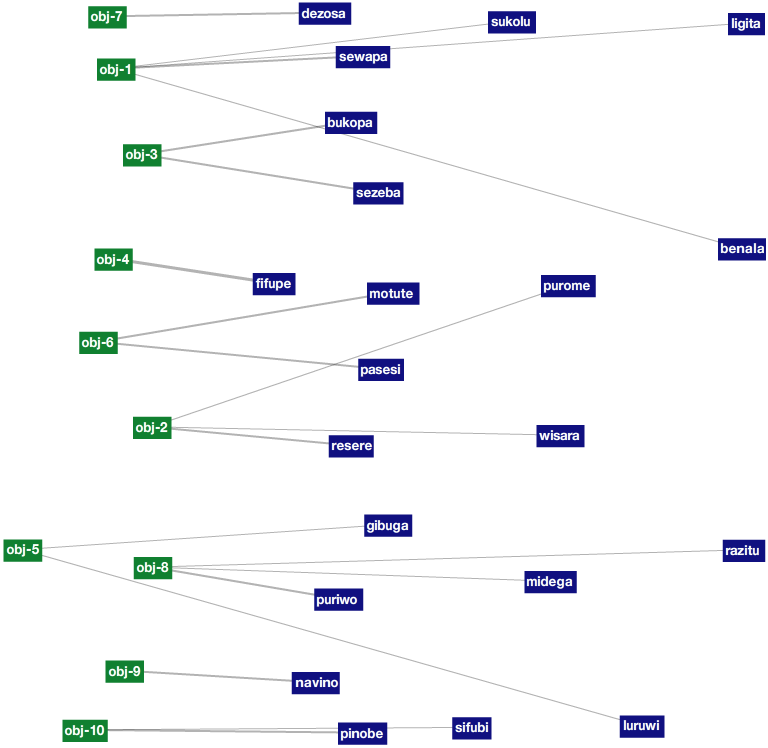
\includegraphics[scale=0.4]{figures/ng-lexicon-250} & &
    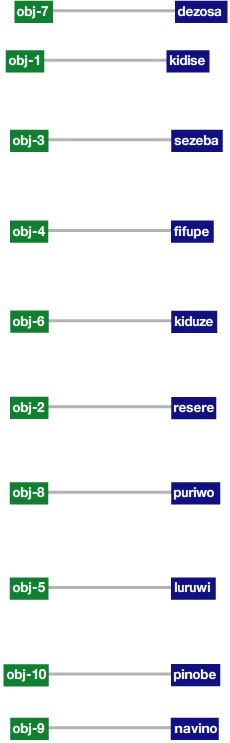
\includegraphics[scale=0.4]{figures/ng-lexicon-2500} \\
    & & \\
  \end{tabular}
  \caption{Network representation of the complete lexicon of the first
    agent in the population after 250 interactions (left) and 2500
    interactions (right). In each network, word meanings are drawn on
    the left and forms on the right. Each line represents a word in
    the lexicon of the agent, the line widths denote the strength of
    the association.}
  \label{f:ng-lexicon}
\end{figure}


Furthermore, even within these few games the population uses three
different forms for \texttt{obj-3}. This is because speakers
independently invent words for new meanings and hearers adopt words
from different speakers for the same meanings. To illustrate this,
Figure \ref{f:ng-lexicon} shows the lexicon of agent 1 after game 250
and after game 2500. After interaction 250, the agent associates up to
five different word forms to each of the meanings, which get reduced
to one per meaning after 2500 interactions. 

\startfiguregroup

\begin{figure}[t]
  
{\renewcommand{\arraystretch}{1.5}
\begin{tabular}{@{}p{1.2cm}|p{1.6cm}@{}p{0.8cm}@{}|p{1.6cm}@{}p{0.8cm}@{}|p{1.6cm}@{}p{0.8cm}@{}|p{1.6cm}@{}p{0.8cm}@{}}
meaning & agent 1 &  & agent 2 &  & agent 3 &  & agent 4 & \\
\hline
\texttt{obj-1}&\textit{``zasala''}


\textit{``milozo''}
&0.50

0.30&\textit{``milozo''}


\textit{``zasala''}
&0.50

0.50&\textit{``botewi''}


\textit{``zasala''}


\textit{``milozo''}


\textit{``legubu''}
&0.50

0.50

0.30

0.30&\textit{``zasala''}


\textit{``botewi''}
&0.30

0.50\\
\hline
\texttt{obj-2}&\textit{``zaxiwu''}
&0.80&\textit{``zaxiwu''}
&0.60&\textit{``dovege''}
&0.40&&\\
\hline
\texttt{obj-3}&\textit{``gokaso''}


\textit{``dotopi''}


\textit{``malixe''}
&0.40

0.40

0.40&\textit{``malixe''}


\textit{``dotopi''}


\textit{``fivine''}
&0.50

0.40

0.50&\textit{``dotopi''}


\textit{``nobaxo''}


\textit{``fivine''}
&0.50

0.40

0.50&\textit{``dotopi''}
&0.30
\end{tabular}}


  \caption{Forms associated to three different meanings by the first
    four agents of a population of 10 after 250 interactions.}
  \label{f:ng-lexicon-250}
\end{figure}

\begin{figure}[t]
  
{\renewcommand{\arraystretch}{1.5}
\begin{tabular}{@{}p{1.2cm}|p{1.6cm}@{}p{0.8cm}@{}|p{1.6cm}@{}p{0.8cm}@{}|p{1.6cm}@{}p{0.8cm}@{}|p{1.6cm}@{}p{0.8cm}@{}}
meaning & agent 1 &  & agent 2 &  & agent 3 &  & agent 4 & \\
\hline
\texttt{obj-1}&\textit{``milozo''}
&1.00&\textit{``milozo''}
&1.00&\textit{``milozo''}
&1.00&\textit{``milozo''}
&1.00\\
\hline
\texttt{obj-2}&\textit{``zaxiwu''}
&1.00&\textit{``zaxiwu''}
&1.00&\textit{``zaxiwu''}
&1.00&\textit{``zaxiwu''}
&1.00\\
\hline
\texttt{obj-3}&\textit{``gokaso''}
&1.00&\textit{``gokaso''}
&1.00&\textit{``gokaso''}
&1.00&\textit{``gokaso''}
&1.00
\end{tabular}}

  \caption{Associations to three meanings after 2000 interactions.}
  \label{f:ng-lexicon-2000}
\end{figure}

\stopfiguregroup

From the perspective of the population, Figure \ref{f:ng-lexicon-250}
shows snapshots of the first four agents' lexicons for three different
meanings after 250 played games. Their lexicons show a very low
coherence, with the numbers of associations and their forms greatly
varying. Whereas all four agents at least already have adopted an
association with the same form for \texttt{obj-2} and \texttt{obj-3}
(``resere'' and ``fodato''), this is not the case for \texttt{obj-1}:
Of all the four forms associated by agent 1 to this meaning, only one
(``sewapa'') is shared with one other agent.

\begin{figure}[t]
  \gnuplotfigure{figures/ng-word-form-scores-obj-3}
  \caption{Evolution of words in the population for the meaning
    \texttt{obj-3}. Each line shows for a single form the
    corresponding word scores averaged over all agents that know the
    form.}
  \label{f:ng-word-form-scores-obj-3}
\end{figure}


\begin{figure}[t]
  \gnuplotfigure{figures/ng-word-form-scores-obj-3-agent-1}
  \caption{Scores for forms associated by the first agent to the
    meaning \texttt{obj-3}.}
  \label{f:ng-word-form-scores-obj-3-agent-1}
\end{figure}


However, due to the strategies of 1) updating word scores based on the
outcome of the game, of 2) laterally inhibiting competing
associations, and of 3) preferring words with higher scores, the
population quickly reaches coherence. Figure \ref{f:ng-lexicon-2000}
shows the lexicons of the same four agents after 2000
interactions. For each of the three meanings, the population agreed on
a single form with 1.0 as the association score. Which of the forms
from the early stages `survives' this selection process can not be
completely determined by looking at the lexicons in Figure
\ref{f:ng-lexicon-250}, but it is clear that associations which are
known to more agents and which have a higher average score in the
population are more likely to become conventionalized.

Figure \ref{f:ng-word-form-scores-obj-3} shows for each form connected
by the population to the meaning \texttt{obj-3} the average
association scores across all agents. The form that eventually wins
(``sezeba'') is created very early on and competes with the form
``bukopa'' for dominance until around interaction 1000, after which
``sezeba'' asserts itself and ``bukopa'' slowly starts loosing the
competition, before it gets eliminated at around interaction 1800. All
other four forms initially created by the population are quickly
lowered in score, and the last one (``wosogi'') is removed by the last
agent at round interaction 900. Nevertheless, individual agents might
undergo much different dynamics. Figure
\ref{f:ng-word-form-scores-obj-3-agent-1} shows the scores of words in
the lexicon of agent 1 for the meaning \texttt{obj-3}. This agent did
not have the winning form ``sezeba'' in his lexicon between
interactions 400 and 500, only after which he re-adopted it and used
it most of the time. Similarly, the already eliminated form ``bukopa''
gets adopted again after interaction 1000 and because agent 1
successfully uses the word one time in the role of the hearer (as
speaker he would have chosen the still higher-scored form ``sezeba''),
the previously more successful ``sezeba'' becomes reduced in score due
to lateral inhibition. 


\begin{figure}[t]
  \gnuplotfigure{figures/ng-word-scores}
  \caption{Evolution of the first agent's lexicon over 2500
    interactions. Each line represents the score of a single word as
    it changes over time.}
  \label{f:ng-word-scores}
\end{figure}

Furthermore, Figure \ref{f:ng-word-scores} shows the evolution of
association scores of all words in the lexicon of agent 1. Despite the
previous example (which is in fact rare), most words that reach a
certain score above the initial words score of 0.5 win the competition
over their competitors and all other words become quickly
removed. After around interaction 1200, the lexicon does not change
anymore and all conventionalized forms remain at a score of 1.\\


\begin{figure}[t]
  \gnuplotfigure{figures/ng-success+lexicon-size}
  \caption{Main dynamics of the Naming Game. Communicative success
    (measure \ref{m:communicative-success}, page
    \pageref{m:communicative-success}) and lexicon size (measure
    \ref{m:lexicon-size}) are averaged over 10 repeated series of 2500
    interactions.}
  \label{f:ng-success+lexicon-size}
\end{figure}

\begin{measure}[b]{Lexicon size}{m:lexicon-size}
  Measures the average number of words known by the population. The
  number of meaning-form associations in each agent's lexicon is
  counted and averaged over the number of agents:
  $$v = \frac{\sum_{i=1}^{|P|} |L(a_i)|}{|P|}$$
  Values $v$ are averaged over the last 250 interactions.
\end{measure}

Finally and most importantly, the alignment dynamics of the population
can be analyzed quantitatively. As already discussed in Section
\ref{s:evaluating-language-games} on page
\pageref{s:evaluating-language-games}, communicative success, i.e. the
fraction of interactions in which the speaker reached his
communicative goal, is our main criterion for evaluating the
performance of language game experiments. Figure
\ref{f:ng-success+lexicon-size} shows the evolution of this measure
over 2500 consecutive interactions: after 600 interactions, in 80\% of
the games communicative success is reached, and after about 1500
interactions, success reaches and remains at 100\%. A second crucial
measure is lexicon size, i.e. the average number of words in the
lexicon of each agent (also shown in Figure
\ref{f:ng-success+lexicon-size}). After an initial phase of invention
and adoption, at around interaction 300, each agent knows about 22
word forms. After that, word score update based on success and lateral
inhibition reduce the number of words, before it reaches 10 at around
interaction 1500. A lexicon size of 10 is considered to be `optimal',
because there are 10 different meanings in the world and an inventory
of 10 words for these meanings is the most cognitively efficient means
to communicate about these meanings in terms of processing and
ambiguities.


\begin{figure}[p]
  \gnuplotfigure{figures/ng-synonymy+coherence}
  \caption{Lexicon coherence (measure \ref{m:lexicon-coherence}),
    frequency of lexicon changes (measure
    \ref{m:frequency-of-lexicon-changes} and average number of forms
    per meaning (measure \ref{m:synonymy}) and averaged over 10
    repeated series of 2500 interactions.}
  \label{f:ng-synonymy+coherence}
\end{figure}


\begin{measure}[p]{Lexicon coherence between speaker and
    hearer}{m:lexicon-coherence}
  Provides a measure for how similar the lexicons of the interacting
  agents are. The degree of lexicon overlap between the speaker $s$
  and the hearer $h$ of the current interaction is computed as the
  fraction of form meaning associations that are shared by speaker and
  hearer and all words known by speaker and hearer:
  $$v=\frac{|L(s) \cap L(h)|}{|L(s)| + |L(h)|}$$
  Association weights of words are ignored when forming the
  intersection between the two lexicons. Values $v$ are averaged over
  the last 250 interactions.\\

  A slightly more precise measure for coherence in the population
  would be to compare the lexicons of all agents. But because
  computing coherence between all pairs of agents would be very
  costly, we chose to use coherence between speaker and hearer as a
  approximation for population coherence.
\end{measure}


\begin{measure}[p]{Frequency of lexicon changes}{m:frequency-of-lexicon-changes}
  Measures how stable the agents' lexicons are. For each interaction
  in which either the speaker or the hearer add or remove a word from
  their inventories, a value of 1 is recorded, for all others
  0. Values are averaged over the last 250 interactions.
\end{measure}


\begin{measure}[p]{Average number of forms per meaning (synonymy)}{m:synonymy}
  The average number of forms associated to each meaning by an agent
  is averaged over all agents in the population:
  $$v = \sum_{i=i}^{|P|}{\frac{|L(a_i)|}{|\{m:m \in {\cal M}\;\wedge\;\exists w ( w \in L(a_i) \wedge m_w(w) = m)  \}|}}\;/\;|P|$$
  Values $v$ are averaged over the last 250 interactions.
\end{measure}

Additionally, we will use measures of coherence, stability, and
ambiguities in inventories for evaluating the performance of language
games in this thesis (see Figure
\ref{f:ng-synonymy+coherence}). Lexicon coherence externally compares
the lexicons of speaker and hearer with respect to how similar they
are in terms of the fraction of shared form-meaning
associations. Coherence reaches 100\% soon after 1500 interactions,
but the curve slightly lags behind communicative success because even
when agents already consistently use the same forms for a particular
meaning, there are still varying competing forms that still need to be
eliminated by lateral inhibition (see also Figures
\ref{f:ng-word-form-scores-obj-3}-\ref{f:ng-word-scores}). 

Frequency of lexicon changes provides a measure for the stability of
the agents' lexicons by counting how often agents add or remove words
in their lexicons. At the beginning, speakers invent words or hearers
adopt words in almost every interaction, and after around interaction
500, when lateral inhibition results in a peak in the number of words
that are removed, the slope of stability increases. But similar to
coherence, complete stability is only reached much later than complete
communicative success (at around interaction 2000), because
lower-scored competing words still need to be removed from the
lexicons.

Finally, the average number of forms associated to each meaning is a
indicator for ambiguities in the agents' lexicons. This measure is
often also referred to as \emph{synonymy}, but the `synonyms' in the
lexicons of our agents are of a different quality than those found in
the real world: here there are competing forms for exactly the same
meaning, whereas in natural languages they are rather seen as words
with similar meanings, but still carrying semantic distinctions. In
the Naming Game, synonymy is directly correlated with lexicon size,
because the number of meanings to be expressed is fixed and there are
no word meaning ambiguities in adoption. The curves for lexicon size
and number of forms per meaning look exactly the same. When lexicon
size peaks at interaction 300 with 22 words, the degree of synonymy is
2.2, and at the optimal size of 10 words, there is only one form per
meaning.


\section{Other alignment strategies \& scaling}
\label{s:ng-alignment-strategies}

The main challenge for aligning lexicons in the Naming Game is the
elimination of competing word forms for the same meanings
(synonymy). The common strategy used for this is to update association
scores based on communicative success and to laterally inhibit
competing forms. However, other strategies are possible and in Figures
\ref{f:ng-alignment-strategy-vs-lexicon-size}-\ref{f:ng-alignment-strategy-vs-lexicon-changes}
we will compare four of them with the update dynamics discussed above
(in the graphs called ``update + lateral inhibition'').

\startfiguregroup

\begin{figure}[t]
  \gnuplotfigure{figures/ng-alignment-strategy-vs-lexicon-size}
  \caption{Compar\-ison of four different alignment strategies: lexicon
    size.}
  \label{f:ng-alignment-strategy-vs-lexicon-size}
\end{figure}

\begin{figure}[t]
  \gnuplotfigure{figures/ng-alignment-strategy-vs-communicative-success}
  \caption{Compar\-ison of four different alignment strategies:
    communicative success.}
  \label{f:ng-alignment-strategy-vs-communicative-success}
\end{figure}

\begin{figure}[t]
  \gnuplotfigure{figures/ng-alignment-strategy-vs-lexicon-changes}
  \caption{Compar\-ison of four different alignment strategies:
    frequency of lexicon changes.}
  \label{f:ng-alignment-strategy-vs-lexicon-changes}
\end{figure}

\stopfiguregroup

First, a strategy that we call ``no alignment'' does not change
association scores at all at the end of an interaction (the parameters
for word score in case of success $\Delta_s$, in case of failure
$\Delta_f$ and for lateral inhibition $\Delta_i$ are all set to
0). But still, although later than with the other strategies, the
population reaches almost complete communicative success after 2500
interactions. Nevertheless, average lexicon size increases to a stable
level of above 50, without ever decreasing again. Since all
associations remain at their initial word score of 0.5, speakers
essentially make a random choice when producing for a specific
meaning. What happens is that every form ever invented by a speaker
needs to be learnt by all other agents in the population in order to
reach success.

The second strategy ``update based on success'' only updates the
associations used by the speaker and hearer for producing and parsing
(and performs no lateral inhibition, $\Delta_s=0.1$, $\Delta_f=-0.1$,
$\Delta_i=0$). Communicative success is reached much faster than with
the default ``update + lateral inhibition'' strategy, but again
lexicon size does not reach the optimum of 10 but remains at a stable
plateau of about 33 words on average. This is because once a form wins
over its competitors, there is no chance for synonyms to be lowered in
score (which in this strategy is only possible through use in a failed
interaction). As a result, a number of `successful' forms for each
meaning will reach a score of 1.0 and speakers will randomly choose
from them, as with the previous strategy. All other associations will
not be used anymore, but remain in the lexicons of the agents.

These `unused' words can be eliminated with the third strategy
``update + constant decay''. In addition to updating scores of used
words based on the outcome of the game with $\Delta_s=0.1$,
$\Delta_f=-0.1$ and $\Delta_i=0$, the score of each association in the
lexicon is changed by a parameter $\Delta_d=-0.05$ divided by the
number of words in the lexicon. When words reach a score of 0 or
below, they are removed from the lexicon. This in a way creates
`blind' lateral inhibition dynamics, since words which are not
successfully used slowly become removed and only words who are
frequently used in successful interactions survive. However, there are
two problems with this strategy. First, the choice of parameter
$\Delta_d$ is very difficult. If it's too high, then words that are
well conventionalized but that happened not to be used often enough
can get accidentally removed. And if it's too low, then synonyms
become removed only very late. Second, this strategy only works when
the meanings expressed by the agents are equally distributed over
time: words for specialized meanings that occur less often are very
unlikely to survive with these dynamics.

Finally, a fourth strategy ``competitor elimination on first success''
again does not update word scores at all. Instead, on the first
occasion that a word is used successfully, all associations with
competing forms are immediately removed from an agent's lexicon (this
behavior can be emulated by choosing the parameters $\Delta_s=0$,
$\Delta_f=0$ and $\Delta_i=-0.5$). Surprisingly, agents reach complete
success and stability also with this strategy, although a bit later
than with the other ones. On the other hand, agents need to remember
less words (lexicon size peaks at about 16) and they don't need to
maintain word scores, which increases cognitive economy, especially
when scaling to larger population sizes.\\

\startfiguregroup

\begin{figure}[t]
  \gnuplotfigure{figures/ng-alignment-delta-inhibit-vs-communicative-success}
  \caption{The impact of different values for the word score update
    parameter $\Delta_i$ on communicative success.}
  \label{f:ng-alignment-delta-inhibit-vs-communicative-success}
\end{figure}

\begin{figure}[t]
  \gnuplotfigure{figures/ng-alignment-delta-inhibit-vs-lexicon-size}
  \label{f:ng-alignment-delta-inhibit-vs-lexicon-size}
  \caption{The impact of different values for the word score update
    parameter $\Delta_i$ on lexicon size.}
\end{figure}

\begin{figure}[t]
  \gnuplotfigure{figures/ng-alignment-delta-fail-vs-communicative-success}
  \label{f:ng-alignment-delta-fail-vs-communicative-success}
  \caption{The impact of different values for the word score update
    parameter $\Delta_f$ on communicative success.}
\end{figure}

\begin{figure}[t]
  \gnuplotfigure{figures/ng-alignment-delta-fail-vs-lexicon-size}
  \label{f:ng-alignment-delta-fail-vs-lexicon-size}
  \caption{The impact of different values for the word score update
    parameter $\Delta_f$ on lexicon size.}
\end{figure}

\begin{figure}[t]
  \gnuplotfigure{figures/ng-alignment-delta-success-vs-communicative-success}
  \label{f:ng-alignment-delta-success-vs-communicative-success}
  \caption{The impact of different values for the word score update
    parameter $\Delta_s$ on communicative success.}
\end{figure}

\stopfiguregroup

\noindent Other alignment strategies such as that the speaker always
imitates the last word heard for a meaning have been investigated by
\cite{kaplan05simple}, and he also found that the default strategy
``update + lateral inhibition'' is the best solution for dampening
competing forms for meanings in the Naming Game. Furthermore, this
strategy is very robust with respect to the actual parameters chosen
for updating word scores. In the literature, the values of
$\Delta_s=0.1$, $\Delta_f=-0.1$ and $\Delta_i=-0.2$ are often been
given some significance, but that choice is not crucial at all. As
shown in Figure
\ref{f:ng-alignment-delta-inhibit-vs-communicative-success}, almost
the same communicative success is reached for parameter $\Delta_i$ for
the whole range of values from 0 to 1. This parameter only affects how
soon agents remove synonyms from their lexicons, and as demonstrated
in Figure \ref{f:ng-alignment-delta-inhibit-vs-lexicon-size}, an
optimal lexicon size is reached quickly for the big range of values
$-1 \leq \Delta_i \leq -0.1$. 

Similarly, actual values for the score update parameter in the case of
communicative failure $\Delta_f$ have no real effect on communicative
success and lexicon size in the range of $-0.2\leq \Delta_i \leq 0$
(see Figures \ref{f:ng-alignment-delta-fail-vs-communicative-success}
and \ref{f:ng-alignment-delta-fail-vs-lexicon-size}). Only when
$\Delta_f$ is too high, then the alignment process has difficulties to
take off, because new words immediately get removed again from an
agent's lexicon on the first occasion that the word was used
unsuccessfully, which can easily happen with new conventions in a
population. Along the same lines, the choice of the association score
update parameter in case of success $\Delta_s$ is quite arbitrary. For
values $0.05 \leq \Delta_s \leq 1$ communicative success is more or
less the same (see Figure
\ref{f:ng-alignment-delta-success-vs-communicative-success}), only
when $\Delta_s$ is too small, negative updates from lateral inhibition
and on communicative failure do not get balanced anymore so that words
have more difficulties to reach high scores.\\

\startfiguregroup

\begin{figure}[t]
  \gnuplotfigure{figures/ng-population-size-vs-communicative-success}
  \label{f:ng-population-size-vs-communicative-success}
  \caption{Scaling of communicative success with increasing population
    size.}
\end{figure}

\begin{figure}[t]
  \gnuplotfigure{figures/ng-population-size-vs-lexicon-size}
  \label{f:ng-population-size-vs-lexicon-size}
  \caption{Scaling of lexicon size with increasing population size.}
\end{figure}

\stopfiguregroup

\noindent Finally, the Naming Game scales very well with increasing
population sizes, as demonstrated in Figures
\ref{f:ng-population-size-vs-communicative-success} and
\ref{f:ng-population-size-vs-lexicon-size}. To keep the curves
comparable, values are plotted along the x axis over the number of
games played by each agent instead of the overall number of
interactions as in the graphs before. For example, for a population of
500 agents to play 100 interactions per agent, $100 * 500 / 2 = 25000$
games need to be played, because two agents take part in every
interaction. The evolution of communicative success takes the form of
a s-curve for all population sizes. After an initial phase with low
success, in which a lot of new forms become invented, more and more
conventions assert themselves and the slope of the curve steepens,
before eventually a plateau of complete success is reached. The curve
for lexicon size looks identical for all population sizes, with
maximums naturally being higher for larger populations, because more
agents independently invent words for the same meanings.

We do not show graphs for scaling with increasing world complexity,
because the Naming Game scales linearly with the number of objects in
the world. With no ambiguity for the hearer in guessing what the
meaning of an unknown word is, the words for each meaning are
negotiated independently. Consequently, aligning words for 20 meanings
in the world takes double as long than for 10 meanings. This is also
the reason for why Naming Game dynamics are often investigated for a
single meaning -- additional meanings do not any complexity to the
model.\\


\noindent Much more is known about the dynamics of Naming Game-like
models of distributed conventionalization processes (in fact, the
Naming Game is by far the most investigated lexicon formation model),
but with lesser relevance for the experiments in our thesis, we will
not discuss these results in depth. There are proofs that the model
always convergences \citep{devylder06how,ke02complexity} (which is
reassuring to know for our work), and convergence times
\citep{kaplan05simple} and scaling laws \citep{baronchelli06sharp} are
well understood. Since it is somehow an unnatural assumption that in
large populations all agents communicate with and learn from each
other with equal probability, the impact of communication network
structures where some agents are more central than others has been
studied by \cite*{dallasta06nonequilibrium}. Furthermore, the
emergence of atomic conventions has been studied in stochastic
game-theoretic frameworks \citep{shoham97emergence}, with Markov
processes \citep{ke02complexity} and in connectionist neural networks
\citep{hutchins95how}. Finally, the impact of stochasticity in
perception, pointing, memory and utterance perception (i.e. there is a
probability of error in transmission) has been investigated by
\cite{steels98stochasticity}.






%%% Local Variables: 
%%% mode: latex
%%% TeX-master: "phd-thesis"
%%% End: 

%% 
\setcounter{chapter}{4}

\chapter{Challenges of ambiguity in word meaning}
\label{c:gg}

\begin{figure}[t]
  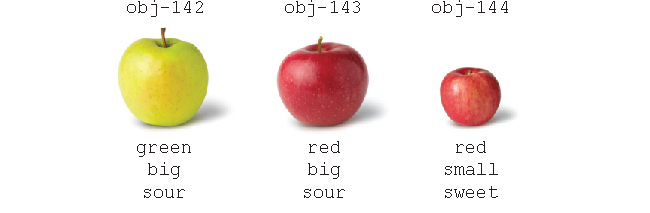
\includegraphics{figures/sgg-example-perception-apples}
  \caption{Example of a simulated world perception. Objects have a
    temporary identifier for establishing reference (\texttt{obj-142},
    \texttt{obj-143}, etc.) and are characterized by a set of
    categories (\texttt{green}, \texttt{big}, etc).}
  \label{f:sgg-example-perception-apples}
\end{figure}

Next we investigate a variety of models that take the Naming Game from
the previous chapter one step further in complexity. Rather than
having the world provide unique categories that then directly become
the meanings underlying an utterance, objects in the world are now
characterized by a set of properties, as shown in the exemplary
context in Figure \ref{f:sgg-example-perception-apples}. Unlike in the
Naming Game, object labels such as \texttt{obj-142}, \texttt{obj-143},
etc. can not be used as meanings, because they do not remain the same
for objects across contexts -- instead they serve as a ``pointer''
that serves as a reference to an object during a game. For setting
objects apart, each of them has a set of properties such as
\texttt{green}, \texttt{big}, and so on. As discussed in Section
\ref{s:representing-linguistic-knowlede}, these properties can be seen
as \emph{categories}, \emph{attributes}, or \emph{features}, and they
are essentially unstructured symbols that are part of the world and
that are thus automatically shared between the agents of the
population. We will call them categories for the remainder of this
thesis.

\pagebreak


In order to draw attention to one of such objects, the speaker needs
to construct a set of categories that allow the hearer to distinguish
the object from all other objects in the context. This process is
called \emph{conceptualization} (see Section
\ref{s:saussure-to-peirce}) and the resulting category set serves as
the meaning that is then verbalized by the speaker. For example in the
scene of Figure \ref{f:sgg-example-perception-apples}, the category
\texttt{green} can be used to distinguish \texttt{obj-142} from all
other objects, because no other object has this property. Similarly,
the categories \texttt{small} and \texttt{sweet} are each sufficient
to discriminate \texttt{obj-144} from the rest. However, only the
combined meanings \texttt{red} $\wedge$ \texttt{big} and \texttt{red}
$\wedge$ \texttt{sour} distinguish \texttt{obj-143} from the other
objects, because each single category of this object is also found in
one of the others.


This additional conceptualization layer creates a variety of further
ambiguities, and the degree of these uncertainties depends on the
nature of word representations (see Section
\ref{s:nature-of-form-meaning-couplings} on page
\pageref{s:nature-of-form-meaning-couplings}). Most importantly, a hearer
perceiving a novel form can not know directly which meaning to
adopt. For example, upon hearing ``fabesi'' for \texttt{obj-144} in
the scene of Figure \ref{f:sgg-example-perception-apples}, the hearer
can infer from the context that the word does not mean \texttt{red}
(because \texttt{obj-143} is also red), but he is left with the
uncertainty whether the speaker meant \texttt{small} or
\texttt{sweet}. Furthermore, when word meanings are not restricted to
single categories but can be structured, the number of potential
meanings multiplies because any discriminating combination of
categories is a meaning candidate. Finally, when utterances are
allowed to contain multiple words, there is the additional uncertainty
in guessing which word carries which meaning. And from the perspective
of a single agent, it is undecidable which words contributed to
communicative failure when updating word scores at the end of a game.\\

\noindent In this chapter we will analyze a number of strategies for dealing
with these challenges. After briefly introducing the world simulation
that we are going to use in Section \ref{s:sgg-world-simulator}, we
will investigate four lexicon formation models that differ in two
aspects. First, whether word meanings are restricted to single
categories (unstructured word meanings) or whether forms can be
associated to sets of categories (structured word meanings). And
second, whether agents can use multiple words to express a meaning
(multi-word utterances) or whether
they use only a single word (single-word utterances):\\

\centerline{
  \begin{tabular}{rcc}
    & single-word utterances & multi-word utterances \\
    unstructured meanings (single categories)  & Section \ref{s:sgg-sw-unstructured} & Section \ref{s:sgg-mw-unstructured} \\
    structured meanings (category sets) & Section \ref{s:sgg-sw-structured} & Section \ref{s:sgg-mw-structured} 
  \end{tabular}}


\section{A simple world simulator}
\label{s:sgg-world-simulator}


A simple world simulation provides our agents with artificial
perceptions such as illustrated in Figure
\ref{f:sgg-example-perception-apples}. In each interaction, a set of
objects $O=\{o_1, o_2, \dots\}$, each containing a number of distinct
categories, is randomly created and perceived by both the speaker and
hearer. The number of objects in a context $O$ is randomly chosen to
be in the range $cs_{min} \leq |O| \leq cs_{max}$. The set of
available categories in the world $C := \{c_1, c_2, \dots\}$ is
constant throughout an experimental run and each object $o \subset C$
consists of a fixed number $|o|$ of categories from $C$ that are
randomly drawn. The world simulator guarantees that no two objects in
a context have the same set of categories.


Throughout this and the next chapter, by default the number of available categories
$|C|$ is 15, the number of categories per object $|o|$ is 10, the
minimum number of objects in a context $cs_{min}$ is 2, and the
maximum context size $cs_{max}$ is 5. An example context that was
created with these parameters is shown below:

\centerline{\small\sffamily
  \begin{tabular}{l|l}
    object & categories \\
    \hline
    \texttt{obj-53} & \texttt{c-4  c-2  c-6  c-12  c-9  c-1  c-14  c-5  c-3  c-15  }\\
    \texttt{obj-54} & \texttt{c-10  c-5  c-11  c-9  c-3  c-2  c-8  c-6  c-7  c-14  }\\
    \texttt{obj-55} & \texttt{c-7  c-5  c-6  c-2  c-15  c-8  c-10  c-13  c-4  c-3  }\\
    \texttt{obj-56} & \texttt{c-10  c-2  c-4  c-7  c-1  c-5  c-6  c-3  c-9  c-13  }\\
  \end{tabular}}




\section{Single words for single categories}
\label{s:sgg-sw-unstructured}

We first look at how populations of agents can agree a set of names
for single categories in language games with single- word
utterances. The additional challenge for reaching coherence compared
to the Naming Game will be that agents will associate word forms to
multiple meanings, in addition to connecting multiple forms to the
same meanings.


\subsection{Conceptualization, interpretation \& the interplay with
  word processing}
\label{s:sgg-sw-unstructured-conceptualization}

Most of the strategies for representing and processing words, for
playing a language game and for learning are identical to those in the
Naming Game (see Section \ref{s:ng-strategies} on page
\pageref{s:ng-strategies}). Here, we will only discuss the
differences.

\inparagraph{Lexicon representation} Form meaning representations are
represented in an identical way as in the Naming Game. The set of
possible word meanings ${\cal M}$ amounts to the set of available
categories in the world $C$.

\inparagraph{Conceptualization} Given the topic chosen by the speaker
and the perceived context, the conceptualization process computes all
categories that part of the topic but not of the other objects. For
example with this context \\

\centerline{\small\sffamily
  \begin{tabular}{l|l}
    object & categories \\
    \hline
    \texttt{obj-3696} & \texttt{c-3  c-15  c-11  c-2  c-6  c-10  c-14  c-4  c-13  c-8  }\\
    \texttt{obj-3697} & \texttt{c-1  c-9  c-13  c-7  c-3  c-8  c-4  c-11  c-6  c-10  }\\
    \texttt{obj-3698} & \texttt{c-2  c-14  c-10  c-11  c-15  c-12  c-5  c-6  c-13  c-8  } \\   
    \multicolumn{2}{l}{}
  \end{tabular}}

\noindent and \texttt{obj-3697} as the topic, conceptualization comes
up with three alternative meanings: \texttt{c-7}, \texttt{c-1} and
\texttt{c-9}. When no such category can be found, then
conceptualization fails, the speaker signals a communicative failure,
and the next interaction starts. 

\begin{figure}[t]
  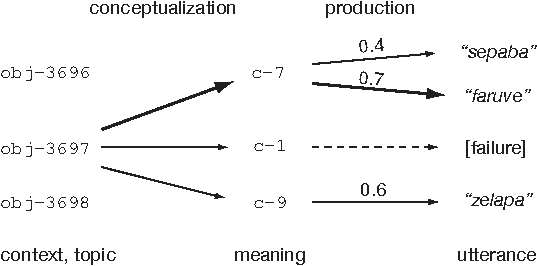
\includegraphics{figures/sgg-semiotic-network-production}
  \caption{Example of a semiotic network in
    production. Conceptualization constructs three different meanings,
    and the lexicon is applied independently to each of them. The path
    that leads to the utterance with the highest word score is drawn
    with a thicker line. }
  \label{f:sgg-semiotic-network-production}
\end{figure}

\inparagraph{Production and the interplay with conceptualization} As
in the Naming Game, the speaker looks up his lexicon for all words
that have the category resulting from conceptualization as their
meaning and from these selects the word with the highest association
score. The difference, however, is that conceptualization often
results in multiple meanings. The lexicon is looked up for each of
them in parallel, and in the end the meaning-utterance combination
with the highest word score is selected. Figure
\ref{f:sgg-semiotic-network-production} illustrates this approach. The
lexicon is independently applied to the three different meanings
\texttt{c-7}, \texttt{c-1} and \texttt{c-9}, and while this agent does
not have a word for \texttt{c-1}, he knows one word for \texttt{c-9}
and two words for \texttt{c-7}. Of all these utterances, ``faruve'' is
then chosen by the speaker because it involved the word with the
highest score of 0.7.

As a consequence of this, it is the lexicon that `selects' the
meanings that are verbalized, which we will later see is a good
strategy. By using the scores of the involved words as a criterion for
which meaning to choose, the speaker increases his chance to be
understood, because higher word scores also mean that the population
reached more consensus about how to name a particular category.


\inparagraph{Invention} Only when production completely fails,
i.e. the speaker does not have a word for any of the conceptualized
meanings, a new word is created for a randomly chosen meaning and
production is retried again.

\begin{figure}[t]
  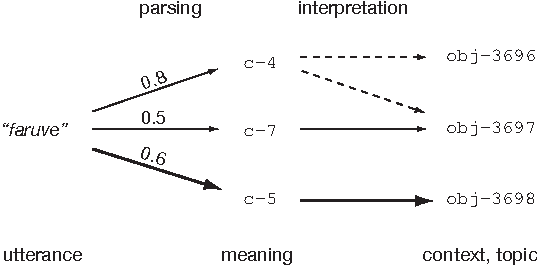
\includegraphics{figures/sgg-semiotic-network-parsing}
  \caption{Example of a semiotic network in parsing. The lexicon of
    this agent contains three different meanings for ``faruve'', which
    are each interpreted independently. The path with the highest word
    score that leads to a single interpreted topic is drawn with a
    thicker line. }
  \label{f:sgg-semiotic-network-parsing}
\end{figure}

\inparagraph{Parsing} The hearer retrieves all words from his own
lexicon that match the utterance. Each of these meanings is then
independently interpreted in the context.

\inparagraph{Interpretation and the interplay with parsing} A meaning
is interpreted in the context by retrieving all objects that share the
category. When multiple objects found for a meaning (and thus the
parsed meaning does not discriminate an object from the rest), then
interpretation for that particular meaning fails. Again, this process
is interconnected with lexicon application. Out of the successful
interpretations, the where the involved form-meaning association has
the highest score is eventually selected. 

An example of this is shown in Figure
\ref{f:sgg-semiotic-network-parsing}. Although the association from
``faruve'' to \texttt{c-4} has the highest score, it is not selected
because the semantic interpretation of \texttt{c-4} results in two
different referents. Instead, the next highest word with the meaning
\texttt{c-5} is chosen, yielding \texttt{obj-3698} as the topic
interpreted by the hearer. Through this, the context constrains
ambiguity in the lexicon by excluding words meanings that are not in
line with the current scene.

\inparagraph{Recovery from failure \& adoption} Three cases are
distinguished when an interaction fails. First, when the hearer could
not come up with a topic (either because he did not know the word or
because interpretation returned multiple objects), then he
re-conceptualizes the scene for the topic pointed at by the speaker
and for each resulting meaning stores an association to the form heard
in his lexicon. Second, when the hearer pointed to the wrong object
(and is consequently corrected by the speaker), then he checks whether
another path in his processing led to the correct topic. For example
in Figure \ref{f:sgg-semiotic-network-parsing}, the alternative path
``faruve'' $\longrightarrow$ \texttt{c-7} $\longrightarrow$
\texttt{obj-3697} would have resulted in the topic intended by the
speaker but was not chosen because the score of the involved word was
not the highest. In such a case, nothing happens and this particular
path is treated specially in consolidation (below). And third, when
the hearer pointed to the wrong object and no other correct path in
processing existed, then the hearer also re-conceptualizes the scene
and adds new words for all the resulting meanings to his lexicon
(except those for which already an association to the form heard
exists).

\begin{figure}[t]
  
\centerline{\footnotesize\renewcommand{\arraystretch}{1.3}{
\begin{tabular}{llllllllc}
  \# & speaker & topic & meaning & utterance & hearer & meaning & topic & success? \\
  \hline
500 & agent 6 & \texttt{obj-1783} &  &  & agent 2 &  &  & no \\
501 & agent 1 & \texttt{obj-1785} & \texttt{c-6} & \textit{``ziraxo''} & agent 8 & \texttt{c-5} & \texttt{obj-1785} & yes \\
502 & agent 1 & \texttt{obj-1787} & \texttt{c-15} & \textit{``wimure''} & agent 9 & \texttt{c-13} & \texttt{obj-1788} & no \\
503 & agent 6 & \texttt{obj-1789} & \texttt{c-15} & \textit{``namuvo''} & agent 5 & \texttt{c-3} &  & no \\
504 & agent 8 & \texttt{obj-1792} &  &  & agent 9 &  &  & no \\
505 & agent 10 & \texttt{obj-1797} & \texttt{c-14} & \textit{``xazapo''} & agent 5 & \texttt{c-14} & \texttt{obj-1797} & yes \\
506 & agent 8 & \texttt{obj-1799} & \texttt{c-9} & \textit{``kugoma''} & agent 9 & \texttt{c-9} & \texttt{obj-1799} & yes \\
507 & agent 7 & \texttt{obj-1803} &  &  & agent 4 &  &  & no \\
508 & agent 7 & \texttt{obj-1805} & \texttt{c-6} & \textit{``ziraxo''} & agent 4 & \texttt{c-6} & \texttt{obj-1805} & yes \\
509 & agent 3 & \texttt{obj-1806} & \texttt{c-8} & \textit{``namuvo''} & agent 9 &  &  & no \\
510 & agent 2 & \texttt{obj-1810} & \texttt{c-1} & \textit{``bikuse''} & agent 4 & \texttt{c-12} &  & no \\
511 & agent 6 & \texttt{obj-1812} &  &  & agent 4 &  &  & no \\
512 & agent 10 & \texttt{obj-1817} & \texttt{c-8} & \textit{``gubawo''} & agent 5 & \texttt{c-4} &  & no \\
513 & agent 8 & \texttt{obj-1819} & \texttt{c-7} & \textit{``vatage''} & agent 10 & \texttt{c-7} & \texttt{obj-1819} & yes \\
514 & agent 6 & \texttt{obj-1822} &  &  & agent 7 &  &  & no \\
 \\\end{tabular}}}


%%% Local Variables: 
%%% mode: latex
%%% TeX-master: "../phd-thesis"
%%% End: 

  \caption{Overview of 15 consecutive interactions from game 500
    on. It shows the agents that are interacting, the topic chosen by
    the speaker, the conceptualized meaning that was chosen, the
    utterance, the meaning parsed by the hearer together with the
    interpreted topic, and whether the agents reached communicative
    success.}
  \label{f:sgg-sw-unstructured-trace}
\end{figure}

\begin{figure}[t]
  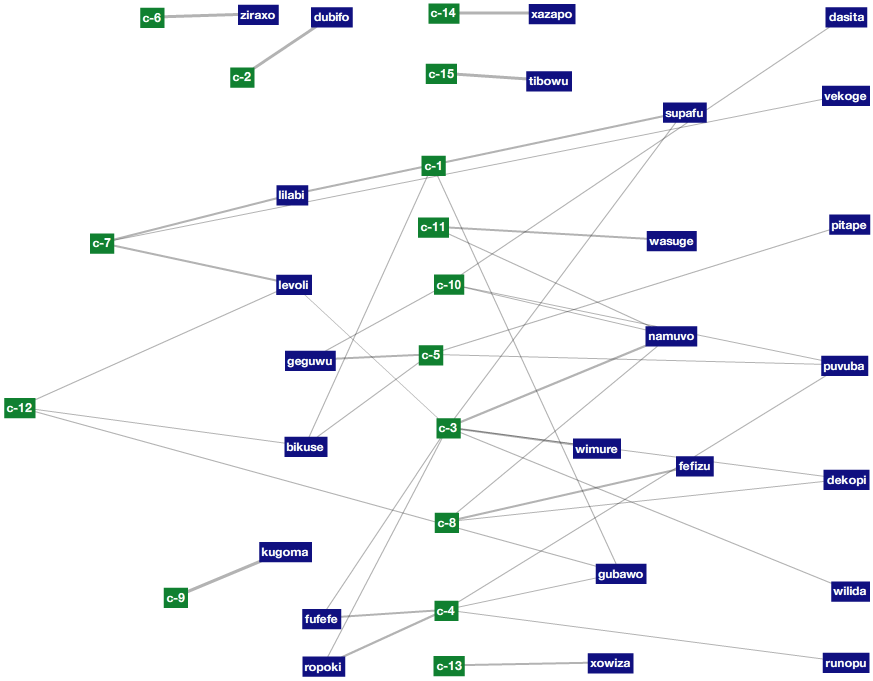
\includegraphics[scale=0.5]{figures/sgg-sw-unstructured-lexicon-1500}
  \caption{Network representation of the complete lexicon of the first
    agent in the population after 1500 interactions. Each line
    represents a word in the lexicon of the agent and connects the
    meaning of the word with its form. The line widths denote the
    strength of the association. }
  \label{f:sgg-sw-unstructured-lexicon-1500}
\end{figure}

\inparagraph{Consolidation} The consolidation strategy is very similar
to the Naming Game. After a failed interaction, the score of the word
used is lowered in score. After a success, the score of the
responsible word increased and those of words with competing forms are
laterally inhibited. The parameters for this update are also the same,
with $\Delta_s=0.1$, $\Delta_f=-0.1$ and $\Delta_i=-0.2$. 

However, there two differences. First, since now there is also the
possibility that multiple meanings are associated to the same form,
they also need to be reduced, which is done using the same lateral
inhibition as for competing forms. Second, when the hearer pointed to
the wrong topic but another path in his processing lead to the correct
topic (as described above), then the score of the word involved is
updated as if the interaction would have been a success (i.e. the
score of the word is increased and words with competing forms or
meanings are inhibited).


\subsection{Dynamics and strategies for reducing ambiguity}
\label{s:sgg-sw-unstructed-strategies}


Figure \ref{f:sgg-sw-unstructured-trace} shows an example of 15
consecutive language games in a population of 10 agents that follow
the strategies described in the previous section. There are a variety
of differences to the Naming Game. First, it can happen that the
speaker is not able to produce an utterance because conceptualization
fails (for example in interaction 500). Second, even when the hearer
is able to parse an utterance, it can happen that non of the resulting
meanings yield a unique object in the context (e.g interaction
503). Third, even when the hearer is able to infer a referent, it
might still be a different one than intended by the speaker
(e.g. interaction 502). And fourth, even when speaker and hearer reach
communicative success, their understanding of the word used might
still be different. For example in interaction 501, the speaker
conceptualizes \texttt{obj-1785} as \texttt{c-6}. The hearer parses
the utterance as \texttt{c-5}, but by chance this gets interpreted as
the same object as intended speaker and consequently, both agents
assume that they used the word ``ziraxo'' correctly and will update
word scores accordingly.



These additional uncertainties are clearly reflected in early states
of the agents' lexicons. Figure
\ref{f:sgg-sw-unstructured-lexicon-1500} shows a snapshot of the
lexicon of the first agent in the population after 1500
interactions. Although this agent has already settled on the forms for
some categories (mostly at the top of the graph), many meanings in
that lexicon are not only linked to multiple forms as before, but
because hearers adopt multiple meanings for forms in the case of
failure, there are also many forms that are connected to multiple
meanings. In order to establish an unambiguous one-to-one mapping of
single forms to single meanings, alignment dynamics need to reduce
these competing forms and meanings over the course of many
interactions.

\startfiguregroup


\begin{figure}[t]
  
{\footnotesize\renewcommand{\arraystretch}{1.5}
\begin{tabular}{@{}p{1.2cm}|p{1.6cm}@{}p{0.8cm}@{}|p{1.6cm}@{}p{0.8cm}@{}|p{1.6cm}@{}p{0.8cm}@{}|p{1.6cm}@{}p{0.8cm}@{}}
meaning & agent 1 &  & agent 2 &  & agent 3 &  & agent 4 & \\
\hline
\texttt{c-1}&\textit{``lilabi''}


\textit{``bikuse''}


\textit{``gubawo''}


\textit{``supafu''}
&0.50

0.20

0.30

0.40&\textit{``dasita''}


\textit{``lazixe''}


\textit{``xowiza''}


\textit{``lilabi''}
&0.40

0.30

0.30

0.20&\textit{``dasita''}


\textit{``lilabi''}


\textit{``bixina''}


\textit{``xowiza''}
&0.50

0.50

0.10

0.40&\textit{``bixina''}


\textit{``namuvo''}


\textit{``vugumi''}


\textit{``lazixe''}


\textit{``bikuse''}


\textit{``ropoki''}


\textit{``runopu''}


\textit{``dekopi''}


\textit{``supafu''}
&0.60

0.30

0.30

0.30

0.20

0.10

0.30

0.30

0.10\\
\hline
\texttt{c-2}&\textit{``dubifo''}
&1.00&\textit{``wimure''}


\textit{``supafu''}


\textit{``fuxefa''}


\textit{``tigasi''}


\textit{``dubifo''}
&0.50

0.50

0.10

0.10

0.50&\textit{``sipuva''}


\textit{``dubifo''}
&0.30

0.50&\textit{``wimure''}


\textit{``vekoge''}


\textit{``vugumi''}


\textit{``lazixe''}


\textit{``dutiru''}


\textit{``dubifo''}
&0.40

0.40

0.50

0.50

0.10

0.50\\
\hline
\texttt{c-3}&\textit{``wimure''}


\textit{``levoli''}


\textit{``fufefe''}


\textit{``namuvo''}


\textit{``supafu''}


\textit{``ropoki''}


\textit{``dekopi''}


\textit{``wilida''}
&0.50

0.30

0.30

0.40

0.30

0.30

0.20

0.20&\textit{``wimure''}


\textit{``vatage''}


\textit{``dekopi''}


\textit{``miwupa''}


\textit{``ropoki''}


\textit{``fuxefa''}


\textit{``bikuse''}


\textit{``puvuba''}


\textit{``namuvo''}
&0.50

0.50

0.50

0.50

0.50

0.50

0.40

0.30

0.40&\textit{``pitape''}


\textit{``gubawo''}


\textit{``miwupa''}


\textit{``geguwu''}


\textit{``sekero''}
&0.50

0.30

0.20

0.60

0.30&\textit{``levoli''}


\textit{``wimure''}


\textit{``vugumi''}


\textit{``supafu''}


\textit{``tigasi''}


\textit{``lazixe''}


\textit{``geguwu''}
&0.50

0.40

0.30

0.30

0.10

0.20

0.20\\
\end{tabular}}

%%% Local Variables: 
%%% mode: latex
%%% TeX-master: "../phdbook"
%%% End: 

  \caption{Forms associated to 3 different meanings by the first four
    agents of a population of 10 after 1500 interactions.}
  \label{f:sgg-sw-unstructured-lexicon-meanings-1500}
\end{figure}

\begin{figure}[t]
  
{\renewcommand{\arraystretch}{1.5}
\begin{tabular}{@{}p{1.2cm}|p{1.6cm}@{}p{0.8cm}@{}|p{1.6cm}@{}p{0.8cm}@{}|p{1.6cm}@{}p{0.8cm}@{}|p{1.6cm}@{}p{0.8cm}@{}}
form & agent 1 &  & agent 2 &  & agent 3 &  & agent 4 & \\
\hline
\textit{``levoli''}&\texttt{c-12}


\texttt{c-7}


\texttt{c-3}
&0.30

0.40

0.30&\texttt{c-12}
&0.40&&&\texttt{c-11}


\texttt{c-7}


\texttt{c-3}


\texttt{c-4}
&0.50

0.50

0.50

0.40\\
\hline
\textit{``lilabi''}&\texttt{c-1}


\texttt{c-7}
&0.50

0.50&\texttt{c-1}
&0.20&\texttt{c-1}
&0.50&\texttt{c-7}
&0.40\\
\hline
\textit{``dubifo''}&\texttt{c-2}
&1.00&\texttt{c-5}


\texttt{c-2}
&0.10

0.50&\texttt{c-2}
&0.50&\texttt{c-11}


\texttt{c-2}
&0.40

0.50\\
\end{tabular}}

%%% Local Variables: 
%%% mode: latex
%%% TeX-master: "../phdbook"
%%% End: 

  \caption{Meanings associated to 3 different forms by the first four
    agents of a population of 10 after 1500 interactions.}
  \label{f:sgg-sw-unstructured-lexicon-forms-1500}
\end{figure}

\stopfiguregroup

\startfiguregroup

\begin{figure}[t]
  
{\footnotesize\renewcommand{\arraystretch}{1.5}
\begin{tabular}{@{}p{1.2cm}|p{1.6cm}@{}p{0.8cm}@{}|p{1.6cm}@{}p{0.8cm}@{}|p{1.6cm}@{}p{0.8cm}@{}|p{1.6cm}@{}p{0.8cm}@{}}
meaning & agent 1 &  & agent 2 &  & agent 3 &  & agent 4 & \\
\hline
\texttt{c-1}&\textit{``lilabi''}
&1.00&\textit{``lilabi''}
&1.00&\textit{``lilabi''}
&1.00&\textit{``lilabi''}
&1.00\\
\hline
\texttt{c-2}&\textit{``dubifo''}
&1.00&\textit{``dubifo''}
&1.00&\textit{``dubifo''}
&0.80&\textit{``dubifo''}
&1.00\\
\hline
\texttt{c-3}&\textit{``geguwu''}
&1.00&\textit{``geguwu''}
&0.90&\textit{``geguwu''}
&1.00&\textit{``geguwu''}
&1.00\\
\end{tabular}}

%%% Local Variables: 
%%% mode: latex
%%% TeX-master: "../phd-thesis"
%%% End: 

  \caption{Forms associated to 3 different meanings by the first four
    agents of a population of 10 after 5000 interactions.}
  \label{f:sgg-sw-unstructured-lexicon-meanings-5000}
\end{figure}

\begin{figure}[t]
  
{\renewcommand{\arraystretch}{1.5}
\begin{tabular}{@{}p{1.2cm}|p{1.6cm}@{}p{0.8cm}@{}|p{1.6cm}@{}p{0.8cm}@{}|p{1.6cm}@{}p{0.8cm}@{}|p{1.6cm}@{}p{0.8cm}@{}}
form & agent 1 &  & agent 2 &  & agent 3 &  & agent 4 & \\
\hline
\textit{``geguwu''}&\texttt{c-3}
&1.00&\texttt{c-3}
&1.00&\texttt{c-3}
&1.00&\texttt{c-3}
&1.00\\
\hline
\textit{``lilabi''}&\texttt{c-1}
&1.00&\texttt{c-1}
&1.00&\texttt{c-1}
&1.00&\texttt{c-1}
&1.00\\
\hline
\textit{``dubifo''}&\texttt{c-2}
&1.00&\texttt{c-2}
&1.00&\texttt{c-2}
&1.00&\texttt{c-2}
&1.00\\
\end{tabular}}

%%% Local Variables: 
%%% mode: latex
%%% TeX-master: "../phdbook"
%%% End: 

  \caption{Meanings associated to 3 different forms by the first four
    agents of a population of 10 after 5000 interactions.}
  \label{f:sgg-sw-unstructured-lexicon-forms-5000}
\end{figure}

\stopfiguregroup


Once more, Figure \ref{f:sgg-sw-unstructured-lexicon-meanings-1500}
compares the forms associated by four agents in the population to
three categories after 1500 interactions. Because the number of
potential word meanings (15 categories) is bigger than in the Naming
Game in the previous chapter (10 objects), and because due to the
uncertainty in meaning the same forms become associated to multiple
categories, there are more competing forms for each category in the
lexicons (compare Figure \ref{f:ng-lexicon-250}, page
\pageref{f:ng-lexicon-250}). Analogously, competing meanings for
three forms in the lexicons of the same four agents are shown in
Figure \ref{f:sgg-sw-unstructured-lexicon-forms-1500}. The degree
of competition between meanings is less than for forms, as we also see
later on. Finally, partial lexicons at the end of the alignment
process are shown in Figure
\ref{f:sgg-sw-unstructured-lexicon-meanings-5000} and
\ref{f:sgg-sw-unstructured-lexicon-forms-5000}. Competing forms and
meaning have been completely eliminated and unambiguous mappings from
single categories to single forms have been established.


\startfiguregroup

\begin{figure}[t]
  \gnuplotfigure{figures/sgg-sw-unstructured-word-form-scores-c-2}
  \caption{Evolution of words with the meaning \texttt{c-2} in the
    population. Each line shows for a single form the corresponding
    word scores averaged over all agents that connect the form to
    \texttt{c-2}. }
  \label{f:sgg-sw-unstructured-word-form-scores-c-2}
\end{figure}

\begin{figure}[t]
  \gnuplotfigure{figures/sgg-sw-unstructured-word-meaning-scores-dubifo-}
  \caption{Evolution of words with the form ``dubifo'' in the
    population. Each line shows for a single meaning the corresponding
    word scores averaged over all agents that associate this meaning
    to ``dubifo''. }
  \label{f:sgg-sw-unstructured-word-meaning-scores-dubifo-}
\end{figure}


\stopfiguregroup

The increased competition between words in the alignment process is
even more visible in the next two graphs. Figure
\ref{f:sgg-sw-unstructured-word-form-scores-c-2} shows the changing
scores of all words in the population with the meaning
\texttt{c-2}. Although the winning form ``dubifo'' is created very
early and although only a few other words are ever used successfully
(i.e. their score increases above the initial word score of 0.5), 25
other forms spread in the population during the first 25000
interactions and slowly become eliminated. Similarly, Figure
\ref{f:sgg-sw-unstructured-word-meaning-scores-dubifo-} shows the
competition of meanings for the form ``dubifo'' in the
population. Before the category \texttt{c-2} eventually wins, the
agents have tried out 10 other meanings.\\


\begin{figure}[t]
  \gnuplotfigure{figures/sgg-sw-unstructured-success+lexicon-size}
  \caption{Main dynamics in a population of 10 agents. Discriminative
    success (measure \ref{m:discriminative-success}), communicative
    success (measure \ref{m:communicative-success}), discriminative
    success on successful discrimination (measure
    \ref{m:communicative-success-given-discriminative-success}) and
    lexicon size (measure \ref{m:lexicon-size}) are averaged over 10
    repeated series of 8000 interactions. }
  \label{f:sgg-sw-unstructured-success+lexicon-size}
\end{figure}

\begin{measure}[b]{Discriminative success}{m:discriminative-success}
  Measures the fraction of interactions in which the speaker was able
  to construct a meaning for the current topic in the context. For
  each interaction with at least one successful conceptualization, the
  value of 1 is recorded, for all others 0. Values are averaged over
  the last 250 interactions.
\end{measure}


\begin{measure}[b]{Communicative success given discriminative
    success}{m:communicative-success-given-discriminative-success}
  Out of the interactions in which the speaker was able to
  conceptualize, measures the fraction of games in which communicative
  success was reached (compare measure \ref{m:communicative-success},
  page \pageref{m:communicative-success}). In all interactions with
  discriminative success, a value of 1 is recorded upon communicative
  success and 0 in the case of failure. In interactions where the
  speaker could not conceptualized, the value of the previous
  interaction is recorded (and 0 in the beginning). Values are
  averaged over the last 250 interactions.
\end{measure}

\noindent The overall performance of a population of 10 agents that
follows the above strategies to agree on forms for single meanings in
single-word utterances is shown in Figure
\ref{f:sgg-sw-unstructured-success+lexicon-size}. First,
discriminative success as a measure for often the speaker is able to
conceptualize the scene is constant at around 55\% through the entire
run. That means that in 45\% of the interactions the scenes computed
by the world simulator (15 categories, 10 categories per object, 2-5
objects per scene) are too ``difficult'' to discriminate the topic
from the other objects using a single category only. Consequently,
communicative success as defined in measure
\ref{m:communicative-success} can only reach the same level as
discriminative success, which it does after about 5000
interactions. In order to still be able to see how successfully the
agents use their linguistic knowledge, we introduce the measure of
communicative success given discriminative success, which basically
`ignores' interactions in which the speaker could not construct a
meaning. This success in language reaches full 100\% after about 5000
interactions. Finally, average lexicon sizes show similar dynamics
compared to the Naming Game. During an initial phase, in which many
words are invented adopted, the average number of form-meaning
associations in each agent's lexicon reaches a peak of slightly over
word. Then, competing forms and meanings become eliminated from the
lexicons, before lexicon size a stable level of 15 words, which is
optimal given that there are 15 categories in the world to express.





\begin{figure}[t]
  \gnuplotfigure{figures/sgg-sw-unstructured-lexicon}
  \caption{Lexicon structure and stability in a population of 10
    agents. The average number of forms per meaning (measure
    \ref{m:synonymy}), the number of meanings per form (measure
    \ref{m:homonymy}), lexicon coherence (measure
    \ref{m:lexicon-coherence} and stability (measure
    \ref{m:frequency-of-lexicon-changes}) are averaged over 10
    repeated series of 8000 interactions.}
  \label{f:sgg-sw-unstructured-lexicon}
\end{figure}


\begin{measure}[b]{Average number of meanings per form
    (homonymy)}{m:homonymy}
  The average number of meanings associated to each form by an agent
  is averaged over all agents in the population:
  $$v= \sum_{i=1}^{|P|}{\frac{|L(a_i)|}{|\{f:f \in {\cal F}\;\wedge\;\exists w ( w \in L(a_i) \wedge f_w(w) = f)  \}|}}\;/\;|P|$$
  Values $v$ are averaged over the last 250 interactions.
\end{measure}


As demonstrated in Figure \ref{f:sgg-sw-unstructured-lexicon}, it
takes much longer to reach full coherence and lexicon stability than
to reach complete communicative success, because even when the
population already agreed on which forms to use for which meanings,
there are still a big number of (now unused) words with competing
forms and meanings left in the lexicons, which only slowly become
removed. At the peak of lexicon size, there are more than four forms
associated to each meaning. And because conceptualization results on
average in 2.6 different meanings (if it succeeds), the average number
of meanings connected to each form reaches about 2.2 at this
point. The number of meanings per form is often also called
`homonymy', but we find this term misleading because in natural
language homonyms tend to coexist in a language, whereas in our
experiments they are subject to competition.\\


\noindent The impact of different alignment strategies for updating
word scores based on the outcome of the game on the performance in
language games is very similar to in the Naming Game (see Section
\ref{s:ng-alignment-strategies} on page
\pageref{s:ng-alignment-strategies}) and we will not analyze it
again. Obviously, competing meanings for forms need to be dampened,
which here underlies the same dynamics as the dampening of competing
forms.

\startfiguregroup


\begin{figure}[t]
  \gnuplotfigure{figures/sgg-sw-unstructured-50-attrs-use-correct-alternative-interpretation-vs-communicative-success}
  \caption{Communi\-cative success in a world of 50 categories for a
    population in which hearers update their lexicons considering
    correct alternative paths in their processing and in which they do
    not.}
  \label{f:sgg-sw-unstructured-50-attrs-use-correct-alternative-interpretation-vs-communicative-success}
\end{figure}

\begin{figure}[t]
  \gnuplotfigure{figures/sgg-sw-unstructured-50-attrs-use-correct-alternative-interpretation-vs-lexicon-size}
  \caption{Lexicon size in a world of 50 categories for a population
    in which hearers update their lexicons considering correct
    alternative paths in their processing and in which they do not.}
  \label{f:sgg-sw-unstructured-50-attrs-use-correct-alternative-interpretation-vs-lexicon-size}
\end{figure}

\stopfiguregroup

We want to highlight the importance of another strategy, especially
since it is usually not incorporated in similar alignment
mechanisms. When the hearer has pointed to the wrong object, he
inspects his parsing and interpretation processing whether another
path through the semiotic network resulted in the correct topic
intended by the speaker (see Section
\ref{s:sgg-sw-unstructured-conceptualization}, paragraph ``Recovery
from failure \& adoption'' above). When this is the case, he does not
re-conceptualize the scene and adopt new meanings, but to the
contrary, treats that path as if it would have been a communicative
success.

Figures
\ref{f:sgg-sw-unstructured-50-attrs-use-correct-alternative-interpretation-vs-communicative-success}
and
\ref{f:sgg-sw-unstructured-50-attrs-use-correct-alternative-interpretation-vs-lexicon-size}
show the impact of using this strategy on communicative success and
lexicon size. To make the difference more clear by increasing
ambiguities in the lexicons, the number of categories in the world has
been set to 50, with the rest of the parameters the same as
before. While communicative success is only slightly higher for agents
that use the strategy over others that do not, the maximum lexicon
size is reduced from about 430 to about 310, and at the same time the
point of maximum lexicon size is reached earlier. Additionally, the
degrees of synonymy and homonymy are also significantly lower and the
lexicon stabilizes more quickly, which all suggests that this strategy
speeds up alignment by reinforcing knowledge that already existed in
their inventories but that was not conventionalized enough to win over
competitors.\\

\startfiguregroup

\begin{figure}[t]
  \gnuplotfigure{figures/sgg-sw-unstructured-50-attrs-conceptualization-handling-vs-communicative-success}
  \caption{The impact of four different strategies for handling
    alternative conceptualizations on communicative success.}
  \label{f:sgg-sw-unstructured-50-attrs-conceptualization-handling-vs-communicative-success}
\end{figure}


\begin{figure}[t]
  \gnuplotfigure{figures/sgg-sw-unstructured-50-attrs-conceptualization-handling-vs-lexicon-size}
  \caption{The impact of four different strategies for handling
    alternative conceptualizations on lexicon size.}
  \label{f:sgg-sw-unstructured-50-attrs-conceptualization-handling-vs-lexicon-size}
\end{figure}


\begin{figure}[t]
  \gnuplotfigure{figures/sgg-sw-unstructured-50-attrs-conceptualization-handling-vs-homonymy}
  \caption{The impact of four different strategies for handling
    alternative conceptualizations on the number of meanings per
    form. The curve for the number of forms per meaning looks very
    similar and is thus not shown.}
  \label{f:sgg-sw-unstructured-50-attrs-conceptualization-handling-vs-homonymy}
\end{figure}

\begin{figure}[t]
  \gnuplotfigure{figures/sgg-sw-unstructured-50-attrs-conceptualization-handling-vs-lexicon-coherence}
  \caption{The impact of four different strategies for handling
    alternative conceptualizations on lexicon coherence.}
  \label{f:sgg-sw-unstructured-50-attrs-conceptualization-handling-vs-lexicon-coherence}
\end{figure}

\begin{figure}[t]
  \gnuplotfigure{figures/sgg-sw-unstructured-50-attrs-conceptualization-handling-vs-lexicon-changes}
  \caption{The impact of four different strategies for handling
    alternative conceptualizations on the frequency of lexicon
    changes.}
  \label{f:sgg-sw-unstructured-50-attrs-conceptualization-handling-vs-lexicon-changes}
\end{figure}

\stopfiguregroup

\noindent Furthermore, the way how alternative conceptualizations are
handled by the speaker and hearer has a dramatic impact on the
dynamics of the language games. First, it matters whether the speaker
tries to apply his lexicon to all meanings that were constructed by
conceptualization (we call this strategy ``speaker: process all''), or
whether he selects a random meaning and applies his lexicon to this
one (``speaker: process one''). As discussed above in Section
\ref{s:sgg-sw-unstructured-conceptualization} (see also Figure
\ref{f:sgg-semiotic-network-production}), all meanings are processed
in parallel by the speaker. Second, it has a big impact whether after
a failure the hearer adopts words for all re-conceptualized meanings
(``hearer: adopt all'', default) or for a random meaning (``hearer:
adopt 1'').

Each of these strategies has their advantages and disadvantages, and
Figures
\ref{f:sgg-sw-unstructured-50-attrs-conceptualization-handling-vs-communicative-success}
--
\ref{f:sgg-sw-unstructured-50-attrs-conceptualization-handling-vs-lexicon-changes}
analyze for all four combinations of them communicative success,
lexicon size, the number of meanings per form, lexicon coherence and
stability in a population of 10 agents. Again, in order to make
differences more visible, the number of categories in the world is 50
instead of 10, which greatly increases ambiguities (as we will discuss
further below).

Communicative success and lexicon stability are reached by far the
quickest when the speaker processes all meanings. Because this allows
speakers to prefer meanings for which he has `good' words that are
already more conventionalized, the population can start to communicate
very successfully about a few meanings. On the downside, it takes
longer for the population to agree on words for all categories in the
world. Only when conceptualization exclusively comes up with meanings
that are not well conventionalized, agents will be forced to
communicate about them, which delays complete alignment. As a
consequence, lexicon coherence rises very slowly (and does not reach
100\% within the 160000 games played) and the frequency of lexicon
changes does not reach 0 for a very long time.


When speakers process only one randomly selected meaning, then it
takes much longer to reach communicative success. The population has
to learn words for all possible meanings simultaneously, which
greatly increases ambiguities and causes high frequencies of lexicon
changes for long periods of time. On the positive side, because all
meanings are tried out with equal change, only with this strategy the
agents can reach 100\% lexicon coherence and complete stability within
the 160000 language games.


Hearers that adopt all re-conceptualized meanings upon recovering from
a communicative failure initially have higher lexicon sizes and higher
degrees of competing forms and meanings, because of course more words
get created in the lexicons of the agents. And it takes much longer
for these measures to reach optimal values, because many new words
become added every time an interaction fails. But surprisingly,
adopting all meanings leads the quickest to success and stability when
combined with the ``speaker: process all'' strategy. When speakers use
meanings with more conventionalized meanings, there is less general
uncertainties and hearers can afford to introduce words for all
meanings and later let the context help to disambiguate between
them. However, when combined with the ``speaker: process 1'' strategy,
then the opposite happens. Ambiguities are so great that words become
added or removed from the lexicons in almost every interaction up to
about game 6000 and it takes the longest to reach communicative
success.

In contrast, when hearers only adopt a word for one randomly selected
re-conceptualized meaning, then lexicon size and form and meaning
ambiguities are much lower. Instead of relying on the lexicon to sort
out the meanings of words through use in different contexts, hearers
make single random guesses and the words immediately disappear again
when they do not by chance are in line with similar guesses by other
agents in the population. But because ambiguities in the lexicon are
avoided, this `random' walk strategy works reasonably well and when
combined with the ``speaker: process 1'' strategy, complete coherence
is reached by far the quickest.


\subsection{Scaling out}

\startfiguregroup

\begin{figure}[t]
  \gnuplotfigure{figures/sgg-sw-unstructured-population-size-vs-communicative-success-given-discriminative-success}
  \caption{Communi\-cative success given discrimination (measure
    \ref{m:communicative-success-given-discriminative-success}) for
    five different population sizes. Results are averaged over 10
    series of varying length, but each with 4000 interactions per
    agent.}
  \label{f:sgg-sw-unstructured-population-size-vs-communicative-success-given-discriminative-success}
\end{figure}


\begin{figure}[t]
  \gnuplotfigure{figures/sgg-sw-unstructured-population-size-vs-lexicon-size}
  \caption{Lexicon size (measure \ref{m:lexicon-size}) for five
    different population sizes. Results are averaged over 10 series of
    varying length, but each with 4000 interactions per agent.}
  \label{f:sgg-sw-unstructured-population-size-vs-lexicon-size}
\end{figure}

\stopfiguregroup

With word meanings being one-to-one mappings between forms and
meanings as in the Naming Game, and with a relatively simple world
simulation (15 categories, 10 categories per object, 2 to 5 objects
per context) the model exhibits similar scaling behavior with
increasing population sizes compared to the Naming Game. Figures
\ref{f:sgg-sw-unstructured-population-size-vs-communicative-success-given-discriminative-success}
and \ref{f:sgg-sw-unstructured-population-size-vs-lexicon-size} show
communicative success given discriminative success and lexicon size
for population sizes from 10 to 200. Success evolves in a similar, yet
flatter s-curve, and lexicon size displays an initial peak that is
slowly reduced in subsequent interactions. The additional ambiguities
in what words mean result in a higher maximum lexicon sizes (e.g. 240
for 100 agents, compared to 55 in the Naming game (although there for
10 meanings, see Figure \ref{f:ng-population-size-vs-lexicon-size} on
page \pageref{f:ng-population-size-vs-lexicon-size}).\\



\startfiguregroup

\begin{figure}[t]
  \gnuplotfigure{figures/number-of-attributes-vs-discriminative-success}
  \caption{Discriminative success (measure
    \ref{m:discriminative-success}) with increasing numbers of
    categories in the world. Results were obtained by running 10
    series of 500 language games and then sampling the average
    discriminative success over the last 250 interactions each.}
  \label{f:number-of-attributes-vs-discriminative-success}
\end{figure}


\noindent Much more interesting is the scaling with increasing
complexity of the world. Figure
\ref{f:number-of-attributes-vs-discriminative-success} demonstrates
that discriminative success increases when more categories available
to the world simulator. When object perceptions are created from
$|C|=40$ categories or more (and the number of categories per scene
remains 10, the number of objects per context 10, and context sizes
between 2 and 5), then object perceptions differ enough so that
speakers can discriminate topics with a single category even for
context sizes of 4 and 5, and consequently discriminative success
reaches 100\%.

\begin{figure}[t]
  \gnuplotfigure{figures/number-of-attributes-vs-number-of-conceptualizations}
  \caption{Number of alternative conceptualizations per scene (measure
    \ref{m:number-of-conceptualizations}) for world simulators with
    increasing number of categories.}
  \label{f:number-of-attributes-vs-number-of-conceptualizations}
\end{figure}

\stopfiguregroup

\begin{measure}[b]{Number of alternative
    conceptualizations}{m:number-of-conceptualizations}
  Measures in how many ways the current topic can be conceptualized in
  the current scene and thus provides a means to quantify referential
  ambiguity. In each interaction in which the speaker is able to
  discriminate the topic from the other objects in the scene, the
  number of resulting meanings is recorded. In case of discriminative
  failure, the value from the previous interaction is recorded
  (initially 0).
\end{measure}


But while discriminative success increases, word meaning ambiguities
also rise in the population. As shown in Figure
\ref{f:number-of-attributes-vs-number-of-conceptualizations}, the
number of different ways how a scene can be conceptualized climbs from
about 2 for 15 categories to almost 8 for 100 categories. This means
that in a world with 15 categories, hearers that try out a newly
adopted word in production have an almost 50\% chance of using the
meaning that was intended by the previous speaker. In a world with 100
categories, this probability is only about 12.5\%.


\startfiguregroup

\begin{figure}[t]
  \gnuplotfigure{figures/sgg-sw-unstructured-number-of-attributes-vs-homonymy}
  \caption{The average number of meanings per form (measure
    \ref{m:homonymy}) for increasing numbers of categories in the
    world. Results are averaged over 10 series of 120000
    interactions.}
  \label{f:sgg-sw-unstructured-number-of-attributes-vs-homonymy}
\end{figure}

The coupling of the number of categories in the world with ambiguity
in re-conceptualization is also clearly reflected in the lexicons of
the agents, as illustrated in Figure
\ref{f:sgg-sw-unstructured-number-of-attributes-vs-homonymy}. For all
different world simulations, the maximum average number of meanings
per form (reached in the initial phase when most words get invented
and adopted) is always about as high as the average number of
alternative conceptualizations.


\begin{figure}[t]
  \gnuplotfigure{figures/sgg-sw-unstructured-number-of-attributes-vs-communicative-success-given-discriminative-success}
  \caption{Communi\-cative success given discriminative success for
    increasing numbers of categories in the world.}
  \label{f:sgg-sw-unstructured-number-of-attributes-vs-communicative-success-given-discriminative-success}
\end{figure}
  
\begin{figure}[t]
  \gnuplotfigure{figures/sgg-sw-unstructured-number-of-attributes-vs-lexicon-size}
  \caption{Lexicon size for increasing numbers of categories in the
    world. The speaker uses a randomly selected conceptualization to
    produce an utterance. }
  \label{f:sgg-sw-unstructured-number-of-attributes-vs-lexicon-size}
\end{figure}

\stopfiguregroup

Despite such high levels of ambiguity, communicative success scales
well with the number of categories in the world and as Figure
\ref{f:sgg-sw-unstructured-number-of-attributes-vs-communicative-success-given-discriminative-success}
shows, communicate success quickly reaches very high levels of over
95\%. However, after an initial steep increase, the curve flattens and
complete success is in fact only achieved for worlds with less than 50
categories (the same holds for coherence, not shown). 

This is due to the default strategy of selecting meanings based on how
well they can be expressed with an agent's lexicon (see above). With
increasing numbers of alternative conceptualizations, speakers can
more easily rely on categories for which well-established forms exist
and avoid those which turned out to be difficult to talk about. As a
consequence, the fraction of categories that are frequently used by
the population decreases, and only when no other conceptualizations
are possible, less conventionalized meanings are used. This, in turn,
slows down the alignment process for these less-frequent categories,
because there are less opportunities to try them out and eliminate
competing forms and meanings. Therefore, the only slowly decreasing
lexicon sizes shown in Figure
\ref{f:sgg-sw-unstructured-number-of-attributes-vs-lexicon-size} are
not in conflict with the high levels of success exhibited in Figure
\ref{f:sgg-sw-unstructured-number-of-attributes-vs-communicative-success-given-discriminative-success}. They
simply reflect the fact that most of the words in the agents lexicon
are only rarely used and are thus not subject to competitor dampening
mechanisms.\\


\startfiguregroup

\begin{figure}[t]
  \gnuplotfigure{figures/sgg-sw-unstructured-speaker-process-one-meaning-number-of-attributes-vs-communicative-success-given-discriminative-success}
  \caption{Communi\-cative success given discriminative success for
    increasing numbers of categories in the world. The speaker uses
    a randomly selected conceptualization to produce an
    utterance. Results are averaged over 10 series of 120000
    interactions.}
  \label{f:sgg-sw-unstructured-speaker-process-one-meaning-number-of-attributes-vs-communicative-success-given-discriminative-success}
\end{figure}


\begin{figure}[t]
  \gnuplotfigure{figures/sgg-sw-unstructured-speaker-process-one-meaning-number-of-attributes-vs-homonymy}
  \caption{Average number of meanings per form for increasing
    numbers of categories in the world. The speaker uses a randomly
    selected conceptualization to produce an utterance. }
  \label{f:sgg-sw-unstructured-speaker-process-one-meaning-number-of-attributes-vs-homonymy}
  \end{figure}


\begin{figure}[t]
  \gnuplotfigure{figures/sgg-sw-unstructured-speaker-process-one-meaning-number-of-attributes-vs-succeeded-with-different-meanings}
  \caption{The fraction of interactions in which communicative success
    is reached although the speaker and hearer used different meanings
    (measure \ref{m:succeeded-with-different-meanings}) for increasing
    numbers of categories in the world. The speaker uses a randomly
    selected conceptualization to produce an utterance. }
  \label{f:sgg-sw-unstructured-speaker-process-one-meaning-number-of-attributes-vs-succeeded-with-different-meanings}
\end{figure}

\begin{measure}[b]{Succeeded with different
    meanings}{m:succeeded-with-different-meanings}
  Measures the fraction of interactions in which agents reached
  communicative success although the hearer parsed the utterance into a
  different meaning than the one that was conceptualized by the
  speaker. After each interaction, the value of 1 is recorded when
  communicative success was reached (see measure
  \ref{m:communicative-success}) and when the meaning that underlies
  the utterance produced by the speaker differs from the meaning that
  was used by the hearer to interpret the topic. Otherwise, a value of
  0 is recorded. Values are averaged over the last 250 interactions.
\end{measure}


\begin{figure}[t]
  \gnuplotfigure{figures/sgg-sw-unstructured-speaker-process-one-meaning-number-of-attributes-vs-lexicon-changes}
  \caption{Frequency of lexicon changes for increasing numbers of
    categories in the world. The speaker uses a randomly selected
    conceptualization to produce an utterance. }
  \label{f:sgg-sw-unstructured-speaker-process-one-meaning-number-of-attributes-vs-lexicon-changes}
\end{figure}

\stopfiguregroup


\noindent Quite different dynamics emerge when speakers are not
allowed to decide which of the alternative conceptualizations to
express in an utterance but when they randomly select a meaning, as
shown in Figures
\ref{f:sgg-sw-unstructured-speaker-process-one-meaning-number-of-attributes-vs-communicative-success-given-discriminative-success}
--
\ref{f:sgg-sw-unstructured-speaker-process-one-meaning-number-of-attributes-vs-lexicon-changes}
(see Section \ref{s:sgg-sw-unstructed-strategies} above for a
discussion of the difference between these strategies). In worlds with
50 categories or less, complete communicative success is reached
within the run of 120000 interactions (Figure
\ref{f:sgg-sw-unstructured-speaker-process-one-meaning-number-of-attributes-vs-communicative-success-given-discriminative-success})
and lexicons are reduced to unambiguous mappings of single forms to
single categories (Figure
\ref{f:sgg-sw-unstructured-speaker-process-one-meaning-number-of-attributes-vs-homonymy}). And
because each category has an equal chance of being used in
communication, the lexicons quickly reach complete stability (Figure
\ref{f:sgg-sw-unstructured-speaker-process-one-meaning-number-of-attributes-vs-lexicon-changes}).

Interestingly, alignment dynamics completely break down for worlds
with more than 50 categories. From 75 categories on, communicative
success stays at a stable level of 25\% and the frequency of lexicon
changes remains at almost 100\%, which means that the lexicons undergo
constant change without reaching any coherence. This is due to the
combination of two factors. First, with increasing numbers of possible
conceptualizations, the chance that the speaker and hearer communicate
successfully but use different meanings also increases. As shown in
Figure
\ref{f:sgg-sw-unstructured-speaker-process-one-meaning-number-of-attributes-vs-succeeded-with-different-meanings},
this happens in 20\% of the successful interactions in worlds with 75
or 100 categories. That also means that in every fifth successful
interaction the agents incorrectly assess whether they used their
words correctly and they will wrongly increase the scores of the
involved words and inhibit scores of competitors. Combined with the
second factor of increased form and meaning ambiguities in the
lexicons (for example the number of meanings per form goes beyond 6
from 75 categories on, Figure
\ref{f:sgg-sw-unstructured-speaker-process-one-meaning-number-of-attributes-vs-homonymy}),
the feedback loop of communicative success on the lexicon collapses
because agents are not able anymore to consistently prefer to use the
right forms for the right meanings.



\section{Holistic coding of structured word meanings}
\label{s:sgg-sw-structured}

Next, we will remove the restriction that word meanings can only be
single categories. With the previous model, agents reached only 55\%
discriminative success, which means that in 45\% of the scenes a
single category was not sufficient to discriminate the topic from the
other objects in the context. To overcome this limitation, we will now
allow agents to construct structured meanings, i.e. sets of categories
that together distinguish an object from the context.

\subsection{Constructing and interpreting compositional meanings}

All strategies for playing the game, production and parsing, learning,
and so on are identical to those of the previous section. The only
difference lies in the way how meanings are constructed and
interpreted and in the extension of word meanings to category sets.

\inparagraph{Conceptualization} The goal of the conceptualization
process is to construct meanings $\{m_1, m_2, \dots\}$ as the minimal
category sets that are part of the topic $o_t \in O$ but that differ
in at least one category from all other objects in the context $O\;\backslash
\;\{o_t\}$:
$$\{m: m \subseteq o_t\; \wedge 
\neg\exists o(o \in O\; \backslash\; o_t \wedge m \subseteq o \}$$
`Minimal' means that the process only yields the shortest category
sets that satisfy the conditions above. In practice, the algorithm
first searches for category sets of length 1, then of length 2, and so
on, until at least one solution is found.

For example, with this as the context\\

\centerline{\small\sffamily
  \begin{tabular}{l|l}
    object & categories \\
    \hline
    \texttt{obj-826} & \texttt{c-11  c-3  c-9  c-13  c-15  c-2  c-4  c-10  c-6  c-14  }\\
    \texttt{obj-827} & \texttt{c-6  c-9  c-14  c-10  c-11  c-3  c-13  c-2  c-8  c-15  }\\
    \texttt{obj-828} & \texttt{c-14  c-6  c-4  c-7  c-15  c-11  c-5  c-9  c-13  c-8  }\\
    \texttt{obj-829} & \texttt{c-3  c-11  c-9  c-12  c-5  c-7  c-14  c-13  c-8  c-6  }\\
    \texttt{obj-830} & \texttt{c-11  c-10  c-9  c-1  c-13  c-14  c-7  c-8  c-15  c-5  }\\
    \multicolumn{2}{c}{ }
  \end{tabular}}

\noindent and \texttt{obj-828} as the topic, conceptualization
constructs the three different meanings \texttt{(c-4 c-8)},
\texttt{(c-4 c-7)} and \texttt{(c-4 c-5)}. The category \texttt{c-4}
is not sufficient to discriminate \texttt{obj-828} from the rest,
because it is also part of \texttt{obj-826}. Only \texttt{c-5},
\texttt{c-7} and \texttt{c-8} are part of the topic, but not of
\texttt{obj-826}, and all other pairs of categories in
\texttt{obj-828} can also be found in other objects.

As a second example, the discrimination of \texttt{obj-904} in the
context\\

\centerline{\small\sffamily
  \begin{tabular}{l|l}
    object & categories \\
    \hline
    \texttt{obj-901} & \texttt{c-14  c-8  c-13  c-10  c-15  c-6  c-5  c-11  c-1  c-12  }\\
    \texttt{obj-902} & \texttt{c-9  c-8  c-5  c-6  c-11  c-10  c-7  c-14  c-3  c-15  }\\
    \texttt{obj-903} & \texttt{c-5  c-1  c-15  c-12  c-4  c-13  c-11  c-9  c-7  c-3  }\\
    \texttt{obj-904} & \texttt{c-10  c-6  c-9  c-13  c-8  c-15  c-12  c-5  c-11  c-14  }\\
    \multicolumn{2}{c}{ }
  \end{tabular}}

\noindent yields eight alternative meanings that each consist of three
categories: \texttt{(c-9 c-13 c-14)}, \texttt{(c-6 c-9 c-12)},
\texttt{(c-10 c-9 c-12)}, \texttt{(c-9 c-12 c-14)}, \texttt{(c-9 c-8
  c-12)}, \texttt{(c-6 c-9 c-13)}, \texttt{(c-10 c-9 c-13)} and
\texttt{(c-9 c-13 c-8)}.


\inparagraph{Structured word meanings} Instead of mapping to single
categories, words are now associations between single forms and sets
of categories, i.e. the space of possible word meanings ${\cal M}$ is
now a subset of all combinations of $C$. Invention, adoption and
alignment are as before.

\inparagraph{Interpretation} Each meaning resulting from parsing is
interpreted in the context by retrieving all objects that share the
categories in the meaning. Again, interpretation of a meaning fails
when multiple topics are found and the path through semiotic network
with the highest word score is eventually selected.


\subsection{Holistic coding as a bad strategy}

Because the world simulation guarantees that each object in the
context differs from all objects in at least one category, the more
powerful conceptualization capabilities lead to 100\% discriminative
success. With the default world simulation parameters, the number of
categories per constructed meaning is one in 55\% of the scenes, two
in 42\% of interactions and three in another 3\%.

For most of the scenes, the number of alternative conceptualizations
is between one and four, but sometimes more than 10 meanings are
conceptualized:\\

{\small\sffamily
  \begin{tabular}{rccccccccccc}
    \# of meanings & 1 & 2 & 3 & 4 & 5 & 6 & 7 & 8 & 9 & 10 & $>$10 \\
    \hline
    frequency & 25\% & 15\% & 16\% & 15\% & 7\% & 7\% & 4\% & 3\% & 3\% & 1\% & 4\% \\
    \multicolumn{12}{c}{ } \\
    \multicolumn{12}{c}{ }
  \end{tabular}}

\begin{figure}[t]
  
\renewcommand{\arraystretch}{1.3}{

\begin{tabular}{@{}llllllllc@{}}
  \# & speaker & topic & meaning & utterance & hearer & meaning & topic & success? \\
  \hline
4500 & agent 5 & \texttt{obj-15741} & \texttt{c-8} & \textit{``timune''} & agent 3 & \texttt{} &  & no \\
4501 & agent 7 & \texttt{obj-15746} & \texttt{c-11} & \textit{``leredi''} & agent 5 & \texttt{c-11} & \texttt{obj-15746} & yes \\
4502 & agent 2 & \texttt{obj-15748} & \texttt{c-14} & \textit{``wekobi''} & agent 4 & \texttt{c-14} & \texttt{obj-15748} & yes \\
4503 & agent 7 & \texttt{obj-15750} & \texttt{c-5 c-4 c-6} & \textit{``budume''} & agent 1 & \texttt{} &  & no \\
4504 & agent 3 & \texttt{obj-15755} & \texttt{c-13 c-1} & \textit{``gikoxe''} & agent 4 & \texttt{c-9 c-5} & \texttt{obj-15757} & no \\
4505 & agent 2 & \texttt{obj-15759} & \texttt{c-8} & \textit{``vafeme''} & agent 4 & \texttt{c-8} & \texttt{obj-15759} & yes \\
4506 & agent 2 & \texttt{obj-15761} & \texttt{c-2} & \textit{``lipuki''} & agent 6 & \texttt{c-2} & \texttt{obj-15761} & yes \\
4507 & agent 7 & \texttt{obj-15764} & \texttt{c-3 c-5} & \textit{``gapeti''} & agent 6 & \texttt{c-13 c-10} & \texttt{obj-15768} & no \\
4508 & agent 6 & \texttt{obj-15769} & \texttt{c-13} & \textit{``madado''} & agent 5 & \texttt{c-13} & \texttt{obj-15769} & yes \\
4509 & agent 10 & \texttt{obj-15772} & \texttt{c-9 c-2} & \textit{``fovodu''} & agent 9 & \texttt{c-9 c-6} & \texttt{obj-15772} & yes \\
4510 & agent 1 & \texttt{obj-15777} & \texttt{c-9 c-10} & \textit{``xesisu''} & agent 2 & \texttt{c-10 c-9} & \texttt{obj-15777} & yes \\
4511 & agent 2 & \texttt{obj-15781} & \texttt{c-7 c-13} & \textit{``wefigu''} & agent 9 & \texttt{c-13 c-7} & \texttt{obj-15781} & yes \\
4512 & agent 10 & \texttt{obj-15790} & \texttt{c-11 c-12} & \textit{``nulafu''} & agent 8 & \texttt{} &  & no \\
4513 & agent 8 & \texttt{obj-15791} & \texttt{c-13 c-10} & \textit{``putoni''} & agent 5 & \texttt{c-3 c-8} & \texttt{obj-15793} & no \\
4514 & agent 4 & \texttt{obj-15795} & \texttt{c-6 c-13} & \textit{``fovodu''} & agent 5 & \texttt{} &  & no \\
4515 & agent 4 & \texttt{obj-15801} & \texttt{c-2} & \textit{``lipuki''} & agent 6 & \texttt{c-2} & \texttt{obj-15801} & yes \\
4516 & agent 3 & \texttt{obj-15805} & \texttt{c-1} & \textit{``pexepo''} & agent 2 & \texttt{} &  & no \\
4517 & agent 5 & \texttt{obj-15807} & \texttt{c-3 c-1} & \textit{``wubimi''} & agent 6 & \texttt{c-3 c-4} & \texttt{obj-15806} & no \\
4518 & agent 10 & \texttt{obj-15811} & \texttt{c-4} & \textit{``vafuxa''} & agent 5 & \texttt{c-4} & \texttt{obj-15811} & yes \\
4519 & agent 7 & \texttt{obj-15815} & \texttt{c-15 c-6} & \textit{``sovota''} & agent 10 & \texttt{c-1 c-8} & \texttt{obj-15813} & no \\
 \end{tabular}}


%%% Local Variables: 
%%% mode: latex
%%% TeX-master: "../phdbook"
%%% End: 

  \caption{Overview of 20 consecutive interactions in a population of
    10 agents from game 4500 on. It shows the agents that are
    interacting, the topic chosen by the speaker, the conceptualized
    meaning that was chosen, the utterance, the meaning parsed by the
    hearer together with the interpreted topic, and whether the agents
    reached communicative success.}
  \label{f:sgg-sw-structured-trace}
\end{figure}

\noindent Nevertheless, using a separate word for each possible
combination of categories is not a very successful strategy for
establishing a communication system. Figure
\ref{f:sgg-sw-structured-trace} gives an example of 20 communicative
interactions in a population of 10 agents. Although already 2500
language games have been played, only about half of the interactions
are successful. Even for single categories some games still fail
(interactions 4500 and 4516) and when multiple categories are
involved, the speaker and the hearer rarely associate the same
meanings to a form.

\begin{figure}[t]
  \gnuplotfigure{figures/sgg-sw-structured-best-best-success+lexicon-size}
  \caption{Communi\-cative success (measure
    \ref{m:communicative-success}), lexicon size (measure
    \ref{m:lexicon-size}) and lexicon coherence (measure
    \ref{m:lexicon-coherence}) in a population of 10 agents. Results
    are averaged over 5 runs of 200000 interactions.}
  \label{f:sgg-sw-structured-best-best-success+lexicon-size}
\end{figure}

\begin{figure}[t]
  \gnuplotfigure{figures/sgg-sw-structured-best-best-lexicon-structure}
  \caption{Lexicon structure and stability. The average number of
    forms per meaning (measure \ref{m:synonymy}), the average number
    of meanings per form (measure \ref{m:homonymy}, the average word
    meaning length (measure \ref{m:average-word-meaning-length}) and
    the frequency of lexicon changes (measure
    \ref{m:frequency-of-lexicon-changes}) are averaged over 5 runs of
    200000 interactions.}
  \label{f:sgg-sw-structured-best-best-lexicon-structure}
\end{figure}


\begin{measure}[b]{Average word meaning length}{m:average-word-meaning-length}
  Measures the average number of categories in the meaning of each
  word of an agent's lexicon averaged over all agents in the
  population:
  $$v=\sum_{i=1}^{|P|}\frac{\sum_{j=1}^{|L(a_i)|}|m(w_j(a_i))|\;/\;|L(a_i)|}{|P|}$$
  Values $v$ are averaged over the last 250 interactions.
\end{measure}


\section{Multi-word utterances for atomic meanings}
\label{s:sgg-mw-unstructured}

Since single-word utterances for structured meanings are obviously a
bad strategy, we will now extend the model to compositional utterances
in which different words cover different parts of the meaning. As an
intermediate step, word meanings are again unstructured as in Section
\ref{s:sgg-sw-unstructured} above, i.e. each word in the utterance
expresses exactly one category. The challenge lies in recovering from
partial processing, that is when a speaker only knows words for some
parts of the meaning or when a hearer only knows meanings for some of
the words in the utterance.


\subsection{Producing and parsing multiple words and learning from
  partial processing}
\label{s:sgg-mw-unstructured-processing}

The strategies for playing the game, conceptualization, interpretation
and alignment are identical to the previous sections and we will again
only highlight the differences. For producing multi-word utterances,
conceptualization of course needs to construct compositional meanings,
i.e. sets of categories as in the previous Section
\ref{s:sgg-sw-structured}. But as already said, word meanings are
again single categories.

\inparagraph{Production} With multiple words expressing different
parts of a meaning $m'$, production is a bit more complicated than a
simple lexicon lookup. First, all applicable words, i.e. words which
express one category of the meaning $A:=\{w: w \in L(a) \wedge m(w)
\in m'\}$ are retrieved from the lexicon. Then, all possible
combinations of these applicable words that do not overlap in meaning
are computed $X := \{x: x \subseteq A \wedge \neg\exists w_1,w_2 (w_1
\in x \wedge w_2 \in x \wedge m(w_1) = m(w_2))\}$, while excluding
solutions that are subsets from other solutions $U = \{u : u \in X
\wedge \neg \exists x (x \in X \backslash u \wedge u \subset
x)\}$. From these combinations, the one with the highest average word
score is selected.

\inparagraph{Invention} When no complete combination of words (i.e.
one that covers all categories in the meaning) can be found for any of
the conceptualized meanings, then the speaker selects the partial
combination that has the least unexpressed categories and the highest
average word score and if there is only one unexpressed category,
invents a new word for it.

\inparagraph{Parsing and interpretation} An utterance $u$ consisting
of several forms $u := \{f_1, f_2, \dots\}$ is parsed by again
retrieving all applicable words $A:=\{w: w \in L(a) \wedge f(w) \in
u\}$, forming combinations that do not overlap in meaning as before
and excluding subsets of other solutions. The meaning underlying an
utterance is formed by concatenating all meanings of a word
combination. Again, all resulting meanings are interpreted in the
context as before and the path leading to a single interpreted object
with the highest average words scores is chosen.

\inparagraph{Re-conceptualization with partial meanings} To recover
from communicative failure, it is again first checked whether another
path in processing lead to the correct topic. If not and if the
utterance contains only a single unknown form, then a new word is
adopted for that form (when there are multiple unknown forms, then
nothing happens, because the ambiguity of which meaning to assign to
which form is too high). In order to determine possible meanings for
the unknown form, the scene is re-conceptualized using the topic
pointed at and the meanings that resulted from the partial parse. That
is, from all constructed meanings only those are considered that
contain all categories from the partial meaning. For all meanings
where the difference between the partial meaning and the meaning
amounts to one category, a new word associating the unknown form to
the category is added to the lexicons of the agents.

\inparagraph{Consolidation \& dampening competing forms and meanings}
The update of category scores is very similar to as before, except
that now multiple words need to be updated. All words that were
involved in producing or parsing the utterance are increased in score
on communicative success and decreased in case of failure and the
competing forms and meanings of the applied words are laterally
inhibited.


\subsection{Interdependent word alignment dynamics}


Multi-word utterances introduce one major additional complexity in the
dynamics of lexicon alignment compared to the models in the previous
Sections \ref{s:sgg-sw-unstructured} and \ref{s:sgg-sw-structured}:
how well a convention spreads in the population does not only depend
on how well it was used in previous interactions, but also on the
other words that is was used with together in an utterance. The
additional challenge that speakers and hearers have to face is the
ambiguity in deciding which word of the utterance were responsible for
communicative failures. 


\begin{figure}[t]
  
\centerline{\footnotesize\renewcommand{\arraystretch}{1.3}{
\begin{tabular}{llllllllc}
  \# & speaker & topic & meaning & utterance & hearer & meaning & topic & success? \\
  \hline
1000 & agent 8 & \texttt{obj-3513} & \texttt{c-1 c-7} & \textit{``sasito kasuvi''} & agent 4 & \texttt{c-13 c-7} & \texttt{obj-3513} & yes \\
1001 & agent 7 & \texttt{obj-3519} & \texttt{c-8 c-7} & \textit{``wuveso lawabe''} & agent 3 & \texttt{c-7 c-12} & \texttt{obj-3517} & no \\
1002 & agent 10 & \texttt{obj-3521} & \texttt{c-12 c-10} & \textit{``sopusa boluto''} & agent 7 & \texttt{c-8 c-2} & \texttt{obj-3523} & no \\
1003 & agent 6 & \texttt{obj-3526} & \texttt{c-9} & \textit{``tibape''} & agent 4 & \texttt{c-2} & \texttt{obj-3526} & yes \\
1004 & agent 2 & \texttt{obj-3528} & \texttt{c-12} & \textit{``fidasa''} & agent 8 & \texttt{c-12} & \texttt{obj-3528} & yes \\
1005 & agent 1 & \texttt{obj-3530} & \texttt{c-7 c-1} & \textit{``dolage lawabe''} & agent 7 & \texttt{c-7 c-4} & \texttt{obj-3532} & no \\
1006 & agent 7 & \texttt{obj-3536} & \texttt{c-6 c-10} & \textit{``ruxize rofoxa''} & agent 4 & \texttt{c-6} &  & no \\
1007 & agent 7 & \texttt{obj-3539} & \texttt{c-8 c-9} & \textit{``sopusa ruxize''} & agent 3 & \texttt{} &  & no \\
1008 & agent 8 & \texttt{obj-3543} & \texttt{c-12} & \textit{``fidasa''} & agent 4 & \texttt{c-2} &  & no \\
1009 & agent 4 & \texttt{obj-3546} & \texttt{c-4 c-1} & \textit{``dolage bofixo''} & agent 3 & \texttt{c-6} &  & no \\
1010 & agent 5 & \texttt{obj-3549} & \texttt{c-6} & \textit{``rofoxa''} & agent 9 & \texttt{c-6} & \texttt{obj-3549} & yes \\
1011 & agent 8 & \texttt{obj-3554} & \texttt{c-5 c-10} & \textit{``lesisi lesisi''} & agent 6 & \texttt{} &  & no \\
1012 & agent 8 & \texttt{obj-3558} & \texttt{c-1 c-8 c-3} & \textit{``zaduba lesisi kasuvi''} & agent 1 & \texttt{c-9 c-11} &  & no \\
1013 & agent 3 & \texttt{obj-3563} & \texttt{c-1 c-7} & \textit{``zepese kurawi''} & agent 2 & \texttt{c-5 c-5} &  & no \\
1014 & agent 6 & \texttt{obj-3565} & \texttt{c-5} & \textit{``zepese''} & agent 9 & \texttt{c-5} & \texttt{obj-3565} & yes \\
 \\\end{tabular}}}


%%% Local Variables: 
%%% mode: latex
%%% TeX-master: "../phd-thesis"
%%% End: 

  \caption{Overview of 15 consecutive interactions from game 1000
    on. It shows the agents that are interacting, the topic chosen by
    the speaker, the conceptualized meaning that was chosen, the
    utterance, the meaning parsed by the hearer together with the
    interpreted topic, and whether the agents reached communicative
    success.}
  \label{f:sgg-mw-unstructured-trace}
\end{figure}

Figure \ref{f:sgg-mw-unstructured-trace} illustrates this by showing
20 consecutive interactions in a population of 10 agents using the
strategies described in the previous section. For example in
interaction 1005, both the speaker and the hearer share the same form
``lawabe`` for the meaning \texttt{c-7}. However, the other word
``dolage`` in the utterance is associated to \texttt{c-1} by the
speaker and to \texttt{c-4} by the hearer. Since the hearer then
interprets the overall meaning as referring to \texttt{obj-3532}, the
interaction leads to a communicative failure. In alignment, both
agents can not know which word was responsible for the
misinterpretation and reduce the scores of both words. It is left to
many subsequent interactions in which the words are used together with
other words to reach coherence in the population.

Similarly, it can happen that agents reach communicative success
although they use different word meanings and consequently falsely
increase the scores of form-meaning associations as the result of a
game. For example in interaction 1000, the speaker conceptualizes the
scene as \texttt{c-1 c-7} and then and the hearer parses the resulting
utterance as \texttt{c-13 c-7}. Since interpretation of that meaning
leads to the same topic \texttt{obj-3513}, speaker and hearer will
both wrongly increase the scores of both words used, also leaving it
to later interactions to home in on the correct meanings.

~\\



\startfiguregroup

\begin{figure}[t]
  \gnuplotfigure{figures/sgg-mw-unstructured-success+lexicon-size}
  \caption{Main measures of alignment. Communicated success (measure
    \ref{m:communicative-success}) and lexicon size (measure
    \ref{m:lexicon-size}) are averaged over 10 repeated series of 6000
    language games.}
  \label{f:sgg-mw-unstructured-success+lexicon-size}
\end{figure}


\begin{figure}[t]
  \gnuplotfigure{figures/sgg-mw-unstructured-lexicon}
  \caption{Evolution of lexicon structure. The average number of forms
    per meaning (measure \ref{m:synonymy}), the number of meanings per
    form (measure \ref{m:homonymy}), lexicon coherence (measure
    \ref{m:lexicon-coherence} and stability (measure
    \ref{m:frequency-of-lexicon-changes}) are averaged over 10
    repeated series of 6000 interactions.}
  \label{f:sgg-mw-unstructured-lexicon}
\end{figure}

\stopfiguregroup

The overall dynamics look very similar to the language games with
single word utterances for single categories in section
\ref{s:sgg-sw-unstructured} (compare Figure
\ref{f:sgg-sw-unstructured-success+lexicon-size}), which is surprising
due to the increased difficulties in lexicon alignment. It can be
however explained with the higher (100\%) discriminative success
resulting from the ability to use multiple categories to conceptualize
a scene, out-weighted by two other factors: First, hearers that
perceive multiple unknown words will not adopt them, since they
associate only one form to one category. And second, a higher number
of interactions needed to resolve the ambiguities mentioned above. As
shown in Figure \ref{f:sgg-mw-unstructured-success+lexicon-size}, the
population reaches 100\% communicative success and an optimal lexicon
size after about 4000 interactions.



For the same reasons as above, the evolution of the lexicon structure
(Figure \ref{f:sgg-mw-unstructured-lexicon}) is also very similar to
the single-category version of the model (compare Figure
\ref{f:sgg-sw-unstructured-lexicon}). The same also holds for all
other alignment dynamics and the scaling with population size and
meaning complexity, which is why we will not repeat them again.


\section{Multi-word utterances and structured meanings}
\label{s:sgg-mw-structured}


We will now come to the language game model game that this chapter has
lead up to: the combination of structured word meanings with
multi-word utterances. It adds one new challenge to the model in the
previous section: There is not only the ambiguity of deciding which
word covers which meanings, but additionally there is the ambiguity in
specificity. Upon hearing a novel word, agents need to decide whether
the word refers to a single category, a combination of categories, or
the complete meaning as a whole.



\subsection{Mapping forms to structured meanings}

Again, most of the strategies for playing the language game are
identical to the previous sections, the main change is to allow word
forms to be associated to sets of categories. 

\inparagraph{Production} Very similar to the strategires described in
Section \ref{s:sgg-mw-unstructured-processing} above for single world
utterances for structured meanings, production means to find the
applicable combination of words that \emph{covers} the meaning $m'$
with the highest average word score. For that, all words whose meaning
is a subset of the meaning to be expressed $A:=\{w: w \in L(a) \wedge
m(w) \in m'\}$ are retrieved from the lexicon. Then, all possible
combinations of these applicable words that do not overlap in meaning
are computed $X := \{x: x \subseteq A \wedge \neg\exists w_1,w_2 (w_1
\in x \wedge w_2 \in x \wedge m(w_1) = m(w_2))\}$, while excluding
solutions that are subsets from other solutions $U = \{u : u \in X
\wedge \neg \exists x (x \in X \backslash u \wedge u \subset
x)\}$. From these combinations, the one with the highest average word
score is selected.


\inparagraph{Invention} When no combination of words in the lexicon of
the speaker can cover the complete meaning, then the partial
combination that has the least unexpressed categories and the highest
average word score is selected and a new word is invented for the
remaining uncovered categories.


\inparagraph{Adoption} Also similarly to as described in Section
\ref{s:sgg-mw-unstructured-processing}, a hearer that doesn't know one
(and only one) of the word forms in the utterance, re-conceptualizes
the scene using the meanings obtained from partially parsing the
utterance. From all parses where such a re-conceptualization is
possible in the current scene, a new word is created associating the
uncovered part to the re-conceptualized meaning.


\subsection{Increased ambiguity in word meanings}


Allowing for structured word meanings while keeping all other
mechanisms for lexicon representation and processing untouched vastly
increases the difficulty for the population to reach a coherent
communication system. Word forms not only compete for the right
category (as in the language games with unstructured meanings) or
holistic meanings that discriminate a topic (as in Section
\ref{s:sgg-sw-structured}), but now they can be associated to an
arbitrary set of categories. 

\begin{figure}[p]
  \rotatebox{90}{
\centerline{\footnotesize\renewcommand{\arraystretch}{1.3}{
\hskip2.0cm\begin{tabular}{llllllllc}
  \\[2.0em]
  \# & speaker & topic & meaning & utterance & hearer & meaning & topic & success? \\
  \hline
500 & agent 8 & \texttt{obj-9728} & \texttt{c-12 c-5} & \textit{``lumase''} & agent 5 & \texttt{c-4 c-5} & \texttt{obj-9728} & yes \\
501 & agent 7 & \texttt{obj-9733} & \texttt{c-14 c-13} & \textit{``zidipa''} & agent 2 & \texttt{c-12 c-10} & \texttt{} & no \\
502 & agent 7 & \texttt{obj-9736} & \texttt{c-4} & \textit{``xatise''} & agent 9 & \texttt{c-13} & \texttt{} & no \\
503 & agent 2 & \texttt{obj-9742} & \texttt{c-10 c-9} & \textit{``vavuro rixate''} & agent 10 & \texttt{c-6} & \texttt{} & no \\
504 & agent 10 & \texttt{obj-9743} & \texttt{c-8} & \textit{``xezibe''} & agent 8 & \texttt{} & \texttt{} & no \\
505 & agent 5 & \texttt{obj-9747} & \texttt{c-15} & \textit{``ritere''} & agent 4 & \texttt{c-9} & \texttt{} & no \\
506 & agent 3 & \texttt{obj-9750} & \texttt{c-1} & \textit{``sobowi''} & agent 10 & \texttt{c-1} & \texttt{obj-9750} & yes \\
507 & agent 10 & \texttt{obj-9753} & \texttt{c-1 c-3} & \textit{``pamadu sobowi''} & agent 5 & \texttt{c-3 c-5} & \texttt{} & no \\
508 & agent 7 & \texttt{obj-9759} & \texttt{c-3 c-9} & \textit{``vevovo''} & agent 9 & \texttt{} & \texttt{} & no \\
509 & agent 8 & \texttt{obj-9766} & \texttt{c-4 c-2} & \textit{``xezibe fukisa''} & agent 2 & \texttt{} & \texttt{} & no \\
510 & agent 2 & \texttt{obj-9771} & \texttt{c-8 c-5 c-3} & \textit{``xozipi kurake nitara''} & agent 3 & \texttt{c-10 c-13 c-15} & \texttt{obj-9767} & no \\
511 & agent 8 & \texttt{obj-9772} & \texttt{c-9} & \textit{``pamadu''} & agent 2 & \texttt{c-6} & \texttt{obj-9772} & yes \\
512 & agent 3 & \texttt{obj-9776} & \texttt{c-3} & \textit{``xuzara''} & agent 1 & \texttt{} & \texttt{} & no \\
513 & agent 1 & \texttt{obj-9777} & \texttt{c-1} & \textit{``gawupa''} & agent 6 & \texttt{} & \texttt{} & no \\
514 & agent 9 & \texttt{obj-9779} & \texttt{c-13 c-14} & \textit{``bogasi manuga''} & agent 2 & \texttt{c-14 c-14} & \texttt{} & no \\
515 & agent 6 & \texttt{obj-9784} & \texttt{c-10 c-6} & \textit{``nitara giberu''} & agent 8 & \texttt{c-6} & \texttt{} & no \\
516 & agent 1 & \texttt{obj-9789} & \texttt{c-1 c-13} & \textit{``liraxe''} & agent 10 & \texttt{} & \texttt{} & no \\
517 & agent 1 & \texttt{obj-9795} & \texttt{c-5 c-13} & \textit{``vavuro fekuvu''} & agent 8 & \texttt{} & \texttt{} & no \\
518 & agent 7 & \texttt{obj-9797} & \texttt{c-11} & \textit{``fufilo''} & agent 10 & \texttt{c-11} & \texttt{obj-9797} & yes \\
519 & agent 1 & \texttt{obj-9800} & \texttt{c-13 c-11} & \textit{``xavaxi''} & agent 7 & \texttt{c-7} & \texttt{} & no \\
\\[2.0em]
 \\\end{tabular}}
}


%%% Local Variables: 
%%% mode: latex
%%% TeX-master: "../phdbook"
%%% End: 


}
  \caption{Overview of 20 consecutive interactions in a population of
    10 agents from game 500 on. It shows the agents that are
    interacting, the topic chosen by the speaker, the conceptualized
    meaning that was chosen, the utterance, the meaning parsed by the
    hearer together with the interpreted topic, and whether the agents
    reached communicative success.}
  \label{f:sgg-mw-structured-trace}
\end{figure}

\startfiguregroup

\begin{figure}[ph]
  
{\footnotesize\renewcommand{\arraystretch}{1.5}
\begin{tabular}{@{}p{1.2cm}|p{1.6cm}@{}p{0.8cm}@{}|p{1.6cm}@{}p{0.8cm}@{}|p{1.6cm}@{}p{0.8cm}@{}|p{1.6cm}@{}p{0.8cm}@{}}
meaning & agent 1 &  & agent 2 &  & agent 3 &  & agent 4 & \\
\hline
\texttt{c-1}&\textit{``fufilo''}


\textit{``furamu''}


\textit{``fukisa''}


\textit{``vepolu''}


\textit{``gawupa''}


\textit{``ninide''}
&0.30

0.30

0.20

0.50

0.20

0.20&\textit{``suniwu''}


\textit{``menula''}


\textit{``ninide''}


\textit{``woxowo''}


\textit{``vepolu''}
&0.50

0.50

0.10

0.40

0.10&\textit{``vepolu''}
&0.80&\textit{``letibe''}


\textit{``gawupa''}


\textit{``vepolu''}
&0.10

0.10

0.60\\
\hline
\texttt{c-2}&\textit{``letibe''}
&0.60&\textit{``wudeso''}
&0.50&\textit{``zoxuko''}


\textit{``dapuvo''}
&0.20

0.40&\textit{``wudeso''}
&0.50\\
\hline
\texttt{c-1 c-2}&\textit{``zilexe''}


\textit{``vekupa''}


\textit{``beleno''}


\textit{``zifuxa''}
&&\textit{``suloko''}
&0.70&\textit{``xomexo''}


\textit{``zepeke''}


\textit{``suloko''}
&0.50&\textit{``fazufi''}
&
\end{tabular}}

  \caption{Forms associated to 3 different meanings by the first four
    agents of a population of 10 after 1500 interactions.}
  \label{f:sgg-mw-structured-lexicon-meanings-1500}
\end{figure}

\begin{figure}[ph]
  
{\renewcommand{\arraystretch}{1.5}
\begin{tabular}{@{}p{1.2cm}|p{1.6cm}@{}p{0.8cm}@{}|p{1.6cm}@{}p{0.8cm}@{}|p{1.6cm}@{}p{0.8cm}@{}|p{1.6cm}@{}p{0.8cm}@{}}
form & agent 1 &  & agent 2 &  & agent 3 &  & agent 4 & \\
\hline
\textit{``zuwika''}&\texttt{c-15}


\texttt{c-8}
&0.50

0.50&\texttt{c-8}
&0.40&&&\texttt{c-8}
&0.50\\
\hline
\textit{``nokuwi''}&\texttt{c-14 c-4}


\texttt{c-15 c-9}


\texttt{c-13 c-14}


\texttt{c-9 c-10}


\texttt{c-14 c-9}
&0.50

0.50

0.50

0.50

0.50&\texttt{c-13 c-5}


\texttt{c-13 c-11}
&0.40

0.50&&&&\\
\hline
\textit{``fufilo''}&\texttt{c-8}


\texttt{c-3}


\texttt{c-10}


\texttt{c-1}
&0.40

0.50

0.30

0.30&\texttt{c-13 c-14}


\texttt{c-6 c-11}


\texttt{c-6 c-13}


\texttt{c-6 c-10}
&0.30

0.50

0.50

0.30&\texttt{c-4}
&0.30&\texttt{c-6 c-11}
&0.20\\
\hline
\textit{``nilebo''}&\texttt{c-3 c-11}


\texttt{c-12 c-11}


\texttt{c-11 c-4}


\texttt{c-14 c-11}


\texttt{c-3 c-7}
&0.50

0.50

0.50

0.50

0.50&\texttt{c-14}
&0.30&\texttt{c-14}


\texttt{c-4}
&0.50

0.50&&\\

\hline
\textit{``fukisa''}&\texttt{c-14}


\texttt{c-1}
&0.50

0.20&\texttt{c-14}
&0.30&\texttt{c-14}
&0.50&\texttt{c-13}


\texttt{c-14}


\texttt{c-5}


\texttt{c-7}
&0.50

0.30

0.10

0.10
\end{tabular}}

  \caption{Meanings associated to 5 different forms by the first four
    agents of a population of 10 after 1500 interactions.}
  \label{f:sgg-mw-structured-lexicon-forms-1500}
\end{figure}

\stopfiguregroup

Consequently, hearers perceiving a novel word need to keep track of a
large number of alternative hypotheses what the word could mean and
hope that these competing meanings get reduced as a result of
subsequent interactions.  This process is made more difficult by the
fact that the meanings that get associated to a novel form depend on
the potentially wrong partial meanings that were retrieved from
partially parsing the known forms in the utterance. For example in
interaction 503 of the series of language games is shown in Figure
\ref{f:sgg-mw-structured-trace}, the speaker conceptualized the topic
as \texttt{c-10 c-9} and the hearer interpreted one of the two words
in ``vaquero rixate'' as \texttt{c-6}. Whatever the re-conceptualized
meaning then was, the hearer will most likely have associated another
meaning to the unknown word than the one that was intended by the
speaker.

Additionally, even when both agents know all the words of the
utterance, they can't know which words were responsible in the case of
a communicative failure. The default strategy of reducing all involved
words in score can be beneficial as in interaction 502 where the
speaker and hearer used the different meanings \texttt{c-14 c-13} and
\texttt{c-12 c-10} for the word ``zidipa'', but there are also other
cases such as interaction 507, when at least one of the words of the
utterance ``pamadu sobowi'' was associated by both agents to the
meaning \texttt{c-3}.

~\\


This uncertainty is clearly reflected in the lexicons of the
agents. Figure \ref{f:sgg-mw-structured-lexicon-meanings-1500} shows
an example of the word forms associated to three different meanings by
four different agents at an early stage of in the evolution of the
population. Whereas at least all of the four agents already somehow
associate ``vepolu'' to the meaning \texttt{c-1}, no agreement
whatsoever exists on the other two meanings \texttt{c-2} and
\texttt{c-1 c-2}. Similarly, the same agents also associate very
different meanings to the same forms in the early stages the language
games (Figure \ref{f:sgg-mw-structured-lexicon-forms-1500}). For
example ``fufilo'' is associated by two agents to single categories,
by the other two to a combinations of two categories -- and non of
these meanings match.

\begin{figure}[p]
  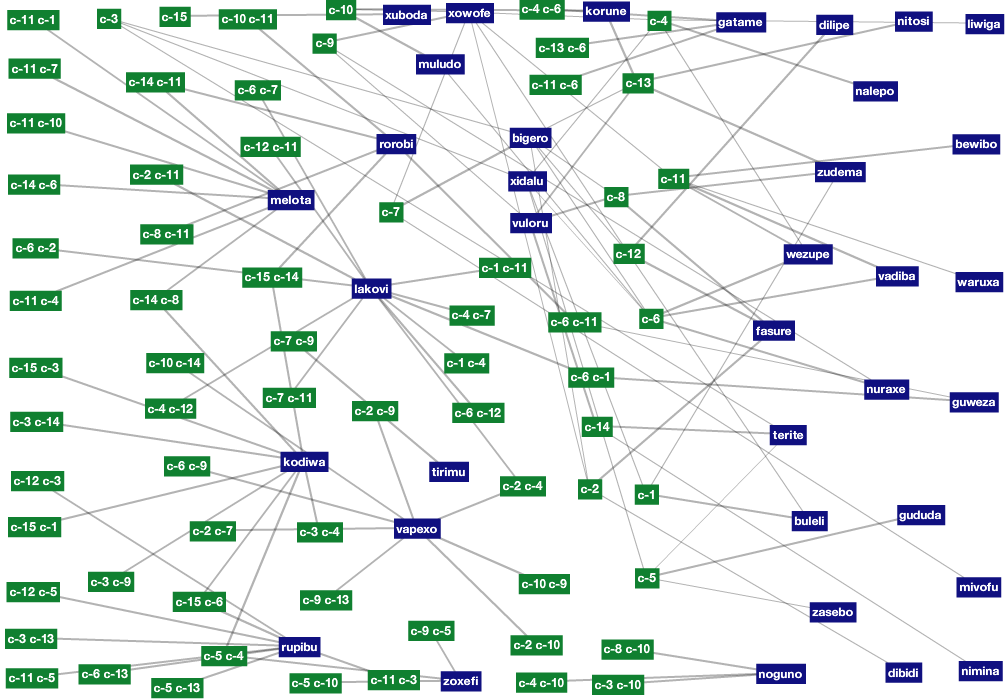
\includegraphics[width=\textwidth]{figures/sgg-mw-structured-lexicon-500}
  \caption{Network representation of the complete lexicon of the first
    agent in the population after 500 interactions. Each line
    represents a word in the lexicon of the agent and connects the
    meaning of the word with its form. The line widths denote the
    strength of the association. }
  \label{f:sgg-mw-structured-lexicon-500}
\end{figure}

\startfiguregroup


\begin{figure}[p]
  \gnuplotfigure{figures/sgg-mw-structured-word-meaning-scores-gesino}
  \caption{Evolution of words with the form ``gesino'' in the
    population. Each line shows for a single meaning the corresponding
    word scores averaged over all agents that associate this meaning
    to ``gesino''. }
  \label{f:sgg-mw-structured-word-meaning-scores-gesino}
\end{figure}

\begin{figure}[t]
  \gnuplotfigure{figures/sgg-mw-structured-word-meaning-scores-xiziwo}
  \caption{Evolution of words with the form ``xiziwo'' in the
    population. }
  \label{f:sgg-mw-structured-word-meaning-scores-xiziwo}
\end{figure}

\stopfiguregroup


Figure \ref{f:sgg-mw-structured-lexicon-500} displays the complete
lexicon of a single agent after 500 interactions. It nicely
illustrates the high number of meanings connected to single forms and
also the high number forms connected to some meanings. In order to
reduce this ambiguity, words need to be tried out in many different
context so that competing forms and meanings can be eliminated through
lateral inhibition. Two typical competition dynamics are given in
Figures \ref{f:sgg-mw-structured-word-meaning-scores-gesino} and
\ref{f:sgg-mw-structured-word-meaning-scores-xiziwo}. The first plots
all the different meanings associated by all the agents in the
population to the form ``gesino'' with their average association
scores. The meaning that eventually wins at around interaction 10000
is \texttt{c-11}, but in the process 36 other competing meanings get
adopted and need to be eliminated. 

A much more typical evolution of a word form is shown in Figure
\ref{f:sgg-mw-structured-word-meaning-scores-xiziwo}. Here, the form
``xiziwo'' attracted 18 different meanings that one after the other
decrease in score until it finally disappears from the population at
around interaction 5500.

~\\

\startfiguregroup

\begin{figure}[t]
  \gnuplotfigure{figures/sgg-mw-structured-success+lexicon-size}
  \caption{Main measures of alignment. Communicated success (measure
    \ref{m:communicative-success}) and lexicon size (measure
    \ref{m:lexicon-size}) are averaged over 10 repeated series of 16000
    language games.}
  \label{f:sgg-mw-structured-success+lexicon-size}
\end{figure}


\begin{figure}[t]
  \gnuplotfigure{figures/sgg-mw-structured-lexicon}
  \caption{Evolution of lexicon structure. The average number of forms
    per meaning (measure \ref{m:synonymy}), the number of meanings per
    form (measure \ref{m:homonymy}), lexicon coherence (measure
    \ref{m:lexicon-coherence} and stability (measure
    \ref{m:frequency-of-lexicon-changes}) are averaged over 10
    repeated series of 16000 interactions.}
  \label{f:sgg-mw-structured-lexicon}
\end{figure}


\stopfiguregroup

The overall dynamics in populations using these kinds of lexicon
representations and learning strategies are given in Figures
\ref{f:sgg-mw-structured-success+lexicon-size} and
\ref{f:sgg-mw-structured-lexicon} and the look very similar to the
ones in the the same diagram for agents using unstructured meanings
from the previous section (see Figures
\ref{f:sgg-mw-unstructured-success+lexicon-size} and
\ref{f:sgg-mw-unstructured-lexicon} on page
\pageref{f:sgg-mw-unstructured-success+lexicon-size}). Complete
communicative success is reached after about 5000 interactions and the
evolution of lexicon size shows the typical shape where first a high
number of words become evented before later alignment reduces many of
them again. 

For reasons that we will briefly discuss in Section
\ref{s:bias-toward-atomic-word-meanings} below, the number of words in
the lexicons of each agent converges to 15, which is also the total
number of categories in the simulated world. Consequently, the average
number of meanings per form and the average number of forms per
meaning also converge to one. The increased ambiguity shows in the
maximum lexicon size of about 160 words that each agent has in its
inventory at around interaction 2000 (compared to about 60 in Figure
\ref{f:sgg-mw-unstructured-lexicon}), a much slower increasing
lexicon coherence and much longer sustained high frequencies of
lexicon changes.


\begin{figure}[t]
  \gnuplotfigure{figures/sgg-mw-structured-misunderstandings+conceptualizations+utterance-length}
  \caption{Causes for ambiguity. The fraction of interactions in which
    communicative success is reached although the speaker and hearer
    used different meanings (measure
    \ref{m:succeeded-with-different-meanings}), the number of
    conceptualizations (measure \ref{m:number-of-conceptualizations})
    and average utterance length (measure \ref{m:utterance-length})
    are averaged over 10 repeated series of 16000 language games.}
  \label{f:sgg-mw-structured-misunderstandings+conceptualizations+utterance-length}
\end{figure}

Some of the challenges that lead to these high uncertainties are
uncertainties in Figure
\ref{f:sgg-mw-structured-misunderstandings+conceptualizations+utterance-length}. The
average number different meanings that can be used to discriminate a
topic from the other objects in the scene is about 4 (because the
world does not change during an experimental run). Furthermore, agents
will communicate successfully while having different understandings of
the meanings in more that 5 percent of the cases during the first 2000
interactions. In this interactions they will wrongly increase the
association scores of the words, while reducing the scores of
competing combinations. And finally, the average utterance length
starts at 1 (the first that speakers will invent cover the complete
uncovered meaning) and gradually converges to 1.5 at around
interaction 2000.


\begin{measure}[t]{Average utterance length}{m:utterance-length}
  Measures the average utterance length, i.e. the number of different
  word forms contained in the utterance produced by the
  speaker. Values are averaged over the last 250 interactions.
\end{measure}


\subsection{The limits of random search}
\label{s:sgg-mv-structured-scaling}

The simulation parameters that were used for the experiments
throughout this chapter are more or less standard in the body of
research that has been done on language game experiments in simulated
environments. The size of the population is 10 agents, simulated world
perceptions consist of two to five objects, each characterized by 10
categories out of an overall fixed set of 15 categories. However, when
increasing the complexity of the scenario slightly beyond these
values, then the strategy of keeping high number of hypotheses of what
words mean in the lexicons of the agents turns out to be a strong
limitation for scaling up. We now briefly analyze the scaling behavior
for increasing population sizes and context sizes.


\startfiguregroup

\begin{figure}[p]
  \gnuplotfigure{figures/sgg-mw-structured-best-best-population-size-vs-lexicon-size}
  \caption{Lexicon size (measure \ref{m:lexicon-size}) for five
    different population sizes. Results are averaged over 10 series of
    varying length, but each with 16000 interactions per agent.}
  \label{f:sgg-mw-structured-best-best-population-size-vs-lexicon-size}
\end{figure}


\begin{figure}[p]
  \gnuplotfigure{figures/sgg-mw-structured-best-best-population-size-vs-lexicon-changes}
  \caption{Frequency of lexicon changes (measure
    \ref{m:frequency-of-lexicon-changes}) for five different population
    sizes. Results are averaged over 10 series of varying length, but
    each with 16000 interactions per agent.}
  \label{f:sgg-mw-structured-best-best-population-size-vs-lexicon-changes}
\end{figure}


\begin{figure}[p]
  \gnuplotfigure{figures/sgg-mw-structured-best-best-population-size-vs-communicative-success}
  \caption{Communi\-cative success (measure
    \ref{m:communicative-success}) for five different population
    sizes. Results are averaged over 10 series of varying length, but
    each with 16000 interactions per agent.}
  \label{f:sgg-mw-structured-best-best-population-size-vs-communicative-success}
\end{figure}

\stopfiguregroup

~\\

The Figures
\ref{f:sgg-mw-structured-best-best-population-size-vs-lexicon-size},
\ref{f:sgg-mw-structured-best-best-population-size-vs-lexicon-changes}
and
\ref{f:sgg-mw-structured-best-best-population-size-vs-communicative-success}
compare lexicon size, frequency of lexicon changes and communicative
success for populations of 10 to 100 agents. In order to be able to
compute these graphs within the memory and computing time limits of
contemporary computer hardware, speakers and hearers use the ``process
1'' respectively ``adopt 1'' strategy for handling alternative
conceptualizations and for adopting word meanings (see page
\pageref{f:sgg-sw-unstructured-50-attrs-conceptualization-handling-vs-lexicon-changes}
et sqq.).

For all five different population sizes, the agents managed to reach
the ``optimal'' lexicon size of 15 words, a stable lexicon that does
not change anymore, and 100\% communicative success. However, reaching
success and coherence takes prohibitively long and agents have to make
huge efforts to align with each other. The average maximum lexicon
size in populations of 100 agents is around 700 words, almost 50 times
as much as the final lexicon size of 15 words. Each agent adds or
removes a word to / from his lexicon in more than 80\% of his first
7000 interactions. And only every tenth out of the first 5000
interactions succeeds. 

It is fair to say that although all involved measures converge, the
alignment strategy of memorizing and later eliminating words does not
scale at all with increasing population size. Agents have to go
through long periods of random search until some words start being
successfully used by a critical fraction of the population. The high
variance across different experimental runs for population sizes above
25 (indicated by the error bars in Figures
\ref{f:sgg-mw-structured-best-best-population-size-vs-lexicon-size},
\ref{f:sgg-mw-structured-best-best-population-size-vs-lexicon-changes}
and
\ref{f:sgg-mw-structured-best-best-population-size-vs-communicative-success})
supports this. In some runs, this ``critical'' moment is reached much
earlier than in others, suggesting that random factors play an
important role in these dynamics. For the case of the Naming Game,
\cite{baronchelli06sharp} have characterized this phenomenon as a
``sharp transition'' from an unordered to an ordered state.

~\\

\startfiguregroup

\begin{figure}[t]
  \gnuplotfigure{figures/sgg-mw-structured-best-best-context-size-vs-number-of-conceptualizations}
  \caption{Number of alternative conceptualizations per scene (measure
    \ref{m:number-of-conceptualizations}) for world simulators with
    increasing number of objects per scene.}
  \label{f:sgg-mw-structured-best-best-context-size-vs-number-of-conceptualizations}
\end{figure}

\begin{figure}[t]
  \gnuplotfigure{figures/sgg-mw-structured-context-size-vs-meaning-length}
  \caption{Average meaning length (measure \ref{m:meaning-length}) for
    world simulators with increasing number of objects per scene.}
  \label{f:sgg-mw-structured-context-size-vs-meaning-length}
\end{figure}

\stopfiguregroup

\begin{measure}[b]{Average meaning length}{m:meaning-length}
  Measures the average meaning length, i.e. the number categories
  contained in the meaning that was conceptualized speaker and used in
  production. Values are averaged over the last 250 interactions.
\end{measure}


For challenging the model with an increasing complexity of the world,
it is enough to increase the number of objects that speakers and
hearers perceive in a single interaction. We chose context size
parameters in such a way that the average number of ways to
conceptualize a scene (and thus the referential uncertainty) stays
more or less the same. Starting from the standard condition in this
chapter in which contexts consisting of 2 to 5 objects, to contexts
with between 5 and 8 objects, there are on average around four
alternative conceptualizations per scene (see Figure
\ref{f:sgg-mw-structured-best-best-context-size-vs-number-of-conceptualizations}).

\startfiguregroup

\begin{figure}[p]
  \gnuplotfigure{figures/sgg-mw-structured-best-best-context-size-vs-lexicon-size}
  \caption{Lexicon size (measure \ref{m:lexicon-size}) for world
    simulators with increasing number of objects per scene. Results
    are averaged over 10 series of 80000 interactions. }
  \label{f:sgg-mw-structured-best-best-context-size-vs-lexicon-size}
\end{figure}


\begin{figure}[p]
  \gnuplotfigure{figures/sgg-mw-structured-best-best-context-size-vs-lexicon-changes}
  \caption{Frequency of lexicon changes (measure
    \ref{m:frequency-of-lexicon-changes}) for world simulators with
    increasing number of objects per scene. Results are averaged over
    10 series of 80000 interactions. }
  \label{f:sgg-mw-structured-best-best-context-size-vs-lexicon-changes}
\end{figure}

\begin{figure}[p]
  \gnuplotfigure{figures/sgg-mw-structured-best-best-context-size-vs-communicative-success}
  \caption{Communi\-cative success (measure
    \ref{m:communicative-success}) for world simulators with
    increasing number of objects per scene. Results are averaged over
    10 series of 80000 interactions. }
  \label{f:sgg-mw-structured-best-best-context-size-vs-communicative-success}
\end{figure}

\stopfiguregroup


Nevertheless, a higher number of objects in a context means that more
categories are needed to discriminate a topic from the other objects
in the context, which is illustrated in Figure
\ref{f:sgg-mw-structured-context-size-vs-meaning-length}. The average
number of categories that speakers need to conceptualize a scene rises
from about 1.5 in contexts of 2 to 5 objects to about 2.2 in contexts
with 5 to 8 objects (see Figure
\ref{f:sgg-mw-structured-context-size-vs-meaning-length}).

This small increase complexity causes a drastic increase in the amount
of work that agents have to do in order to keep track of word
meanings, leading to an even worse scaling behavior than with
population size (see Figures
\ref{f:sgg-mw-structured-best-best-context-size-vs-lexicon-size},
\ref{f:sgg-mw-structured-best-best-context-size-vs-lexicon-changes}
and
\ref{f:sgg-mw-structured-best-best-context-size-vs-communicative-success}). Only
for the first two world simulator configurations (perceived contexts
consist of between 2 and 5 objects, respectively 2 and 6 objects) the
population of again 10 agents is able to reach complete success and
lexicon stability. The high variance indicated by the error bars
across different runs for contexts with between 3 and 6 objects
indicates that in this case the population was able to converge in
some of the runs whereas in others not. Anyway, for all other
configurations, the lexicon representation and the strategies for
alignment simply don't work.



\subsection{Bias towards atomic word meanings}
\label{s:bias-toward-atomic-word-meanings}

Although the agents are endowed with the capacity to represent and
process compositional word meanings, the lateral inhibition dynamics
used by the agents to gradually reduce alternative hypotheses
constitute a bias towards unstructured word meanings. 

\startfiguregroup

\begin{figure}[t]
  
{\footnotesize\renewcommand{\arraystretch}{1.5}
\begin{tabular}{@{}p{1.2cm}|p{1.6cm}@{}p{0.8cm}@{}|p{1.6cm}@{}p{0.8cm}@{}|p{1.6cm}@{}p{0.8cm}@{}|p{1.6cm}@{}p{0.8cm}@{}}
meaning & agent 1 &  & agent 2 &  & agent 3 &  & agent 4 & \\
\hline
\texttt{c-1}&\textit{``vepolu''}
&1.00&\textit{``vepolu''}
&1.00&\textit{``vepolu''}
&1.00&\textit{``vepolu''}
&1.00\\
\hline
\texttt{c-2}&\textit{``letibe''}
&1.00&\textit{``letibe''}
&1.00&\textit{``letibe''}
&1.00&\textit{``letibe''}
&1.00\\
\hline
\texttt{c-1 c-2}&\textit{``beleno''}

\textit{``zifuxa''}
&0.10

0.10&\textit{``suloko''}
&0.20&&&&
\end{tabular}}

  \caption{Forms associated to 3 different meanings by the first four
    agents of a population of 10 after 5000 interactions.}
  \label{f:sgg-mw-structured-lexicon-meanings-5000}
\end{figure}

\begin{figure}[t]
  
{\renewcommand{\arraystretch}{1.5}
\begin{tabular}{@{}p{1.2cm}|p{1.6cm}@{}p{0.8cm}@{}|p{1.6cm}@{}p{0.8cm}@{}|p{1.6cm}@{}p{0.8cm}@{}|p{1.6cm}@{}p{0.8cm}@{}}
form & agent 1 &  & agent 2 &  & agent 3 &  & agent 4 & \\
\hline
\textit{``xavuto''}&\texttt{c-8}
&0.50&\texttt{c-8}
&0.70&\texttt{c-8}
&0.30&\texttt{c-8}
&0.60\\
\hline
\textit{``buxoxo''}&\texttt{c-8}
&0.10&\texttt{c-8}
&0.10&&&&\\
\hline
\textit{``vewuxa''}&\texttt{c-13}
&1.00&\texttt{c-13}
&1.00&\texttt{c-13}
&1.00&\texttt{c-13}
&1.00\\
\hline
\textit{``vaxutu''}&\texttt{c-3 c-12}
&1.00&\texttt{c-3}
&1.00&\texttt{c-3}
&1.00&\texttt{c-3}
&1.00\\
\hline
\textit{``godefe''}&\texttt{c-11 c-8}


\texttt{c-13 c-8}


\texttt{c-13 c-3}
&0.30

0.50

0.50&\texttt{c-14 c-9}


\texttt{c-2 c-14}
&0.30

0.30&&&\texttt{c-13 c-6}
&0.20\\
\end{tabular}}

  \caption{Meanings associated to 3 different forms by the first four
    agents of a population of 10 after 5000 interactions.}
  \label{f:sgg-mw-structured-lexicon-forms-5000}
\end{figure}

\stopfiguregroup

The lexicon snapshots of the same four agents from Figures
\ref{f:sgg-mw-structured-lexicon-meanings-1500} and
\ref{f:sgg-mw-structured-lexicon-forms-1500} but 3500 interactions
later at interaction 5000 (Figures
\ref{f:sgg-mw-structured-lexicon-meanings-5000} and
\ref{f:sgg-mw-structured-lexicon-forms-5000}) illustrate this. All
four agents agreed on the same forms ``vepolu'' and ``letibe'' for the
atomic meanings \texttt{c-1} and \texttt{c-2} and all converged to the
highest score of 1.0 for these associations. On the contrary, there is
no conventionalized form for the structured meaning \texttt{c-1 c-2}
and the three words that remained in the population have very low
association scores. Looking form the other direction, word forms that
are connected to single categories are so with higher scores than
those that map to structured meanings. An interesting and rare
exception is the form ``vaxutu''. While all other agents connect the
meaning \texttt{c-3} to it, the first agent uses the two categories
\texttt{c-3 c-12}.


The explanation for this effect is something that
\cite{debeule06compositionality} called a frequency effect. Lateral
inhibition after a successful language game operates equally on all
words that also could have been applied, and consequently words
connected to single categories have an advantage in these dynamics. In
the example above, the words expression the category combination
\texttt{c-1 c-2} are in direct competition with the words expressing
\texttt{c-1} or \texttt{c-2} for all conceptualizations that contain
these two categories. However, words expressing \texttt{c-1 c-2} can
only be used in such situations, whereas words expressing single
categories can be used in a much wider variety of contexts (basically
all conceptualizations that contain that category). They thus can be
tried out more frequently, and consequently can spread more quickly
the population and be part of more successful interactions. Which
means that they will have higher combined scores than their structured
counterparts and finally win the competition over them.



% \subsection{Structure in the world}

%%% Local Variables: 
%%% mode: latex
%%% TeX-master: "thesis"
%%% End: 

%% 
\setcounter{chapter}{5}

\chapter{Flexible representations for word learning}
\label{c:flexible}


Without antedating the discussion of the results of the previous
chapter (this will be happen in Chapter \ref{c:chapter-11}), we want
to highlight two major shortcomings. First, it is a bad strategy to
enumerate many alternative hypotheses about what words mean in the
lexicons of the agents. Because the conceptualized structured meanings
can be any subset of the available categories, referential uncertainty
exponentially increases with the number of categories. Turning this
into an exponentially increasing competition between word meanings
does not scale. Second, the alignment dynamics of the experiments in
the previous chapters contain a bias towards atomic words
meanings. However, in natural language words are not only about single
categories such as red or small but most of them carry complex
structured meanings, a fact that a lexicon representation should be
able to capture.


\begin{figure}[t]
  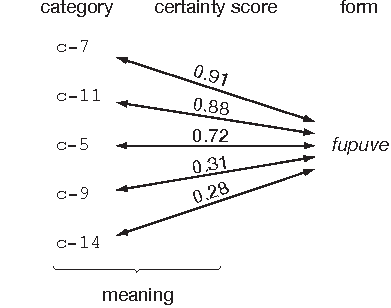
\includegraphics[width=0.43\linewidth]{figures/fwm-word}
  \caption{Illustration of a single flexible word representation. The
    form ``fupuve'' is associated to 5 different categories with
    individual certainty scores. }
\label{f:fwm-word}
\end{figure}


The lexicon formation model introduced in this chapter tries to
address these two shortcomings by capturing uncertainty in the
representation of word meanings themselves\footnote{Some parts of this
  chapter (mainly Section \ref{s:sfwm-representations}) are adapted
  from \cite*{wellens08flexible}, see also
  \cite{wellens07flexible,wellens12multi-dimensional}}. Instead of
having competing mappings to different sets of categories for the same
word, words now have flexible connections to different categories that
are constantly shaped by language use. This is achieved by keeping an
\emph{(un)certainty score} for every category in a form-meaning
association instead of scoring the meanings as a whole (Figure
\ref{f:fwm-word}). This representation is strongly related to both
fuzzy set theory \citep{zadeh65fuzzy} with the degree of membership
interpreted as the degree of (un)certainty, and prototype theory
\citep{rosch73natural}.  Although this representation is identical to
a fuzzy set, in what follows, we refer to the representation as a
\emph{weighted set} to avoid confusion since we will redefine many set
theoretic operations.  By allowing the certainty scores to change, the
representation becomes adaptive and the need to explicitly enumerate
competing hypotheses disappears.




\section{Processing and aligning flexible word representations}
\label{s:sfwm-representations}


Again, the overall strategies for playing language games are identical
to those in the previous two chapters. Also, the same simulated world
from the experiments in the previous chapter is used. Interacting
agents jointly perceive a simulated scene consisting of 2 to 5
objects, which themselves are represented by subsets from a list of 15
categories. We repeat here an example context of such joint perception
from Section \ref{s:sgg-world-simulator} (page
\pageref{s:sgg-world-simulator}):

\centerline{\small\sffamily
  \begin{tabular}{l|l}
    object & categories \\
    \hline
    \texttt{obj-53} & \texttt{c-4  c-2  c-6  c-12  c-9  c-1  c-14  c-5  c-3  c-15  }\\
    \texttt{obj-54} & \texttt{c-10  c-5  c-11  c-9  c-3  c-2  c-8  c-6  c-7  c-14  }\\
    \texttt{obj-55} & \texttt{c-7  c-5  c-6  c-2  c-15  c-8  c-10  c-13  c-4  c-3  }\\
    \texttt{obj-56} & \texttt{c-10  c-2  c-4  c-7  c-1  c-5  c-6  c-3  c-9  c-13  }\\
  \end{tabular}}

~\\

The difference to the experiments in the previous two chapters lies in
the nature of word representations and how they are processed,
invented, adopted and aligned.


\inparagraph{Weighted sets} Perceptions of objects and words in the
lexicon have \emph{weighted sets} as the same underlying
representation. This allows for example production processes to use a
\emph{similarity} measure to find the best combination of words that
expresses a topic. Each weighted set is a list of mappings of a
category (denoted \texttt{category} below) to a real-valued
\emph{certainty score} between $0$ and $1$ (called \texttt{certainty} in
the remainder of this section).

\inparagraph{Similarity between weighted sets} It is possible to
define a weighted similarity measure for the above representation,
taking the certainty scores as weights. Given two weighted sets of
categories as input, the measure returns a real number between $-1$
and $1$, respectively denoting disjunction and equality. This weighted
similarity measure lies at the core of the model and requires detailed
elaboration but we first need to define some additional functions.
Assume a function \texttt{Categories(A)} that takes as input a
weighted set $A$ and returns the normal set $B$ containing only the
categories from $A$, and a function \texttt{CertaintySum(A)} that
takes as input a weighted set $A$ and returns a real number
representing the sum of all the certainty scores.  We can then define
the following operations as slight modifications from those in fuzzy
set theory:

\begin{verbatim+}
\textbf{Function} Intersection(A, B):

\textbf{ForEach} (category \& certainty) \textbf{in} A
    \textbf{If} Find category \textbf{in} Categories(B)
    \textbf{then} Add (category \& certainty) \textbf{to} intersection;
\textbf{End ForEach};

\textbf{Return} intersection;
\end{verbatim+}


\begin{verbatim+}
\textbf{Function} Difference(A, B):

\textbf{ForEach} (category \& certainty) \textbf{in} A
    \textbf{If} not Find category \textbf{in} Categories(B)
    \textbf{then} Add (category \& certainty) \textbf{to} difference
\textbf{End ForEach};

\textbf{Return} difference;
\end{verbatim+}


\noindent Note that in contrast to its definition in fuzzy set theory,
function \texttt{Intersection} is not commutative because it returns
all shared categories between $A$ and $B$ but with certainty scores from
$A$.  With these definitions we can define the weighted similarity
measure as follows:

\begin{verbatim+}
\textbf{Function} Similarity(A, B):

sharedSum $\leftarrow$ CertaintySum(Intersection(A, B)) 
                $\times$ CertaintySum(Intersection(B, A);
diffSum $\leftarrow$ CertaintySum(Difference(A, B) 
              $\times$ CertaintySum(Differenc(B, A));
similarity $\leftarrow$ (sharedSum - diffSum) 
                  / CertaintySum(A) $\times$ CertaintySum(B);

\textbf{Return} similarity;
\end{verbatim+}


\noindent Given two weighted sets $A$ and $B$, \texttt{Similarity} first takes
all shared categories and all disjoint categories between $A$ and $B$. By
using the \texttt{CertaintySum} function we allow the certainty scores
to weight in. It is clear that sharing categories is beneficial for
the similarity and not sharing categories is not. Intuitively,
\texttt{Similarity(A,B)} will be higher the more categories are shared
between $A$ and $B$ and the higher their certainty scores
are. Correspondingly, the more categories are not shared by $A$ and
$B$ and the higher their certainty scores, the lower the result will
be. Some examples:


\begin{verbatim+}
Similarity(((a 1.0) (b 0.5) (c 0.7)), ((a 0.5) (b 0.5) (c 0.7))) 
     = (2.2 $\times$ 1.7 - 0 $\times$ 0) / 2.2 $\times$ 1.7 = 1 
    
Similarity(((a 1) (b 1) (c 1)), ((d 1) (e 1) (f 1))) 
    = (0 $\times$ 0 - 3 $\times$ 3) / 3 $\times$ 3 = -1
    
Similarity(((a 0.9)), ((a 1) (b 0.1) (c 0.2))) 
    = (0.9 $\times$ 1 - 0 $\times$ 0.02) / 0.9 $\times$ 1.3 = 0.77
    
Similarity(((a 0.5) (b 0.5) (c 0.5)), ((a 0.5) (c 0.5) (d 0.5))) 
    = (1 $\times$ 1 - 0.5 $\times$ 0.5) / 1.5 $\times$ 1.5 = 0.33
\end{verbatim+}

\inparagraph{Conceptualization} In the experiments in the previous
chapter, agents conceptualized a scene by finding minimal sets of
categories that \emph{discriminate} the topic from the rest of the
objects in the scene. To allow for more adaptive alignment dynamics,
this now is part of lexicon application. For this, all the objects in
the scene are converted to weighted sets, with constant certainty
scores of $0.5$.

\inparagraph{Production} A speaker that tries to produce gradually
adds words to the utterance so that the combined words are most
similar to the topic and most dissimilar to the other object in the
context:

\begin{verbatim+}
\textbf{Function} Produce(context, topic, lexicon):

bestNewWord $\leftarrow$ nil; \textit{// the current best new candidate word} 
utterance $\leftarrow$ nil; \textit{// The utterance will gradually be combined in here} 
productionScores $\leftarrow$ nil;

\textbf{Loop}
    \textbf{ForEach} word \textbf{in} (lexicon $\setminus$ words in utterance) \textbf{do}
        meaningOfUtterance $\leftarrow$ FuzzySetUnion(\textbf{ForEach} word \textbf{in} utterance
                                            \textbf{collect} Meaning(word));
        meaningOfExtendedUtterance $\leftarrow$ FuzzySetUnion(meaningOfUtterance 
                                                    + Meaning(word));
        objectSimilarities 
            $\leftarrow$ \textbf{ForEach} object \textbf{in} context 
                  \textbf{collect} Similarity(meaningOfExtendedUtterance, 
                                     object));

        topicSimilarity 
            $\leftarrow$ GetSimilarity(topic, objectSimilarities);
        closestOtherSimilarity 
            $\leftarrow$ Max(objectSimilarities $\setminus$ topicSimilarity);
        Add (topicSimilarity $-$ closestOtherSimilarity) 
            \textbf{to} productionScores;
    \textbf{End ForEach};
    bestNewWord $\leftarrow$ word with highest score in productionScores;
    \textbf{If} ProductionScore(bestCandidate) 
        $>$ average of ProductionScores(utterance)
        \textbf{then} Add bestNewWord \textbf{to} utterance;
        \textbf{Else} \textbf{Break} from Loop;
\textbf{End Loop};

\textbf{Return} utterance;
\end{verbatim+}

\noindent The \texttt{ForEach} loop will fill
\texttt{productionScores} with a score for each unused word in the
lexicon denoting not just its similarity to the topic but taking into
account its similarity to the rest of the context. For example if the
topic is a red object, but all other objects in the context are also
red it doesn't really help that much to use the word red. The
\texttt{bestNewWord} is thus the word with the highest score in
\texttt{productionScores}. If the productionScore for
\texttt{bestNewWord} improves the average of the
\texttt{productionScores} for the \verb+utterance+ so far it gets
added to the \texttt{utterance}, if not the search stops. In the end
\texttt{utterance} is that subset of the lexicon that strikes the
optimal balance between being most similar to the topic and being most
distant from the other objects of the context. This results in context
sensitive multi-word utterances and involves an implicit on-the-fly
discrimination using the lexicon.


\inparagraph{Interpretation} Parsing an utterance amounts to looking
up the meaning of all uttered words, taking the fuzzy union (as
defined in \citealp{zadeh65fuzzy}) of their categories and measuring
similarity between this set and every object in the context:

\begin{verbatim+}
\textbf{Function} Interpret(utterance, context):

interpretedMeaning 
    $\leftarrow$ Fuzzy Union of all meanings for known words in utterance;
objectSimilarities 
    $\leftarrow$ \textbf{ForEach} object \textbf{in} context 
                     \textbf{collect} Similarity(interpretedMeaning, object);
topic $\leftarrow$ object with highest score in objectSimilarities;

\textbf{If} similarityScore of topic $>$ 0
    \textbf{then} \textbf{Return} topic;
\end{verbatim+}

\inparagraph{Invention} After finding the best possible combination of
words to describe the topic, the speaker first interprets his own
utterance himself. In this process -- which is also called
\emph{re-entrance} \citep{steels03re-entrance} -- the speaker takes
himself as a model of the hearer and thus can check potential
misinterpretations, allowing him to rephrase or remedy the
utterance. When re-entrance leads the speaker to a different object
than his own, which means that no combination of words can
discriminate the topic in the current context, refinement of the
lexicon is needed.  The speaker invents a new form and associates to
it, with very low initial certainty score, all so far unexpressed
categories of the topic. Because word meanings can shift, it might not
be necessary to introduce a new word. Chances are that the lexicon
needs a bit more time to be shaped further. Therefore the more similar
the meaning of the utterance is to the topic, the less likely a new
word will be introduced:

\begin{verbatim+}
\textbf{Function} Invention(utterance, topic, context):

interpretedTopic $\leftarrow$ Interpret(utterance, context);
\textbf{If} interpretedTopic $\neq$ topic
\textbf{then}
    interpretedSimilarity $\leftarrow$ Similarity(utterance, interpretedTopic);
    topicSimilarity $\leftarrow$ Similarity(utterance,topic);
    randomNr $\leftarrow$ Random($0$ $1$) \textit{// A random number between 0 and 1}
    \textbf{If} (interpretedSimilarity $-$ topicSimilarity) > randomNr
    \textbf{then} 
        newMeaning $\leftarrow$ Categories of (topic $\setminus$  Meaning(utterance)) 
        newWord $\leftarrow$ makeWord(randomString, newMeaning);
        \textbf{Return} newWord;
\end{verbatim+}


\inparagraph{Adoption} When the hearer encounters one or more novel
words in the utterance, then he needs a way to associate an initial
representation of meaning with the novel forms. For that, the first
interprets the words he knows and tries to play the game without
adopting the novel forms. At the end of the game, when he knows the
topic from communicative feedback, the hearer associates all
unexpressed categories with all novel forms. Just as in invention, the
initial certainty scores start out very low, capturing the uncertainty
of this initial representation. Excluding the categories of the
already known words is the only constraint shaping the initial
representation. Note that there is no explicit enumeration of
competing interpretations:

\begin{verbatim+}
\textbf{Function} Adoption(utterance, topic, novelForms):

newMeaning $\leftarrow$ Categories of (topic $\setminus$  Meaning(utterance))
\textbf{ForEach} form \textbf{in} novelForms \textbf{do} 
    Add makeWord(form, newMeaning) \textbf{to} lexicon; 
\end{verbatim+}


\inparagraph{Alignment} After each interaction, the speaker and hearer
determine which parts of the meanings of the used words were
beneficial (the ones shared with the topic) and which not (the
disjoint categories): 

\begin{verbatim+}
\textbf{Function} Align(agent, topic, utterance)

topicCategories $\leftarrow$ Categories(topic);
sharedCategories $\leftarrow$ Categories(utterance) $\cap$ topicCategories;
disjointCategories $\leftarrow$ Categories(utterance) $\setminus$ topicCategories;
 
\textit{// Update certainty scores}
\textbf{ForEach} word \textbf{in} utterance 
   \textbf{ForEach} category \textbf{in} Meaning(word) 
      \textbf{If} category in sharedCategories
      \textbf{then} IncrementScore(word, category);
      \textbf{Else} DecrementScore(word, category); 
           \textit{// Also removes categories if score < 0} 
\textbf{If} not CommunicatedSuccessfully(agent) 
\textbf{then} \textit{// Make words more specific, only the hearer does this} 
   \textbf{ForEach} word \textbf{in} utterance 
      \textbf{do} Associate disjointCategories to word;
\end{verbatim+}

Certainty scores are slightly shifted every time a word is used in
production or interpretation. The certainty score of the categories
that raised the similarity are incremented (\emph{entrenchment}) and
the others are decremented \emph{erosion}. Categories with a certainty
score equal or less than 0 are removed, resulting in a more general
word meaning. In failed games the hearer adds all unexpressed
categories of the topic, again with very low certainty scores, to all
uttered words, thus making the meanings of those words more specific.



\section{Continuous shaping of word meanings}

\begin{figure}[p]
  \rotatebox{90}
  {
\footnotesize\renewcommand{\arraystretch}{1.35}{
  \begin{tabular}{p{0.4cm}p{1.4cm}p{7cm}p{7cm}p{1.4cm}p{0.6cm}}
    \noalign{\vskip 0.5cm}
  \# & speaker + topic & word meanings speaker & word meanings hearer & hearer + topic & succ. \\
  \hline



500 & agent 7 

\texttt{obj-1495} &\textit{"satitu"} (\texttt{c-2}\textsuperscript{.19}, \texttt{c-1}\textsuperscript{.10}, \texttt{c-3}\textsuperscript{.10}, \texttt{c-13}\textsuperscript{.10}, \texttt{c-5}\textsuperscript{.10}, \texttt{c-6}\textsuperscript{.03}, \texttt{c-8}\textsuperscript{.02}, \texttt{c-4}\textsuperscript{.02}, \texttt{c-11}\textsuperscript{.02})

\textit{"fobigu"} (\texttt{c-7}\textsuperscript{.27}, \texttt{c-5}\textsuperscript{.11}, \texttt{c-8}\textsuperscript{.10}, \texttt{c-4}\textsuperscript{.10}, \texttt{c-11}\textsuperscript{.10}) & \textit{"satitu"} (\texttt{c-8}\textsuperscript{.20}, \texttt{c-5}\textsuperscript{.20}, \texttt{c-2}\textsuperscript{.10}, \texttt{c-1}\textsuperscript{.10})

\textit{"fobigu"} (\texttt{c-7}\textsuperscript{.22}, \texttt{c-8}\textsuperscript{.20}, \texttt{c-4}\textsuperscript{.13}, \texttt{c-3}\textsuperscript{.05}) & agent 3 

 \texttt{obj-1495} & yes \\
501 & agent 1 

\texttt{obj-1497} &\textit{"satitu"} (\texttt{c-5}\textsuperscript{.26}, \texttt{c-1}\textsuperscript{.26}, \texttt{c-11}\textsuperscript{.17}, \texttt{c-4}\textsuperscript{.17}, \texttt{c-10}\textsuperscript{.13}) & \textit{"satitu"} (\texttt{c-5}\textsuperscript{.29}, \texttt{c-8}\textsuperscript{.20}) & agent 6 

 \texttt{obj-1497} & no \\
502 & agent 7 

\texttt{obj-1499} &\textit{"xamexu"} (\texttt{c-8}\textsuperscript{.17}, \texttt{c-14}\textsuperscript{.17}, \texttt{c-12}\textsuperscript{.17}, \texttt{c-15}\textsuperscript{.17})

\textit{"bovaze"} (\texttt{c-8}\textsuperscript{.20}, \texttt{c-5}\textsuperscript{.20}, \texttt{c-9}\textsuperscript{.17}, \texttt{c-1}\textsuperscript{.11})

\textit{"dugobo"} (\texttt{c-6}\textsuperscript{.17}, \texttt{c-1}\textsuperscript{.17}, \texttt{c-3}\textsuperscript{.06}) & \textit{"xamexu"} (\texttt{c-8}\textsuperscript{.20}, \texttt{c-12}\textsuperscript{.17}, \texttt{c-11}\textsuperscript{.04}, \texttt{c-13}\textsuperscript{.02}, \texttt{c-7}\textsuperscript{.02})

\textit{"bovaze"} (\texttt{c-8}\textsuperscript{.32}, \texttt{c-9}\textsuperscript{.32}, \texttt{c-1}\textsuperscript{.24}, \texttt{c-10}\textsuperscript{.02}, \texttt{c-7}\textsuperscript{.02})

\textit{"dugobo"} (\texttt{c-1}\textsuperscript{.20}, \texttt{c-5}\textsuperscript{.10}, \texttt{c-6}\textsuperscript{.10}) & agent 6 

 \texttt{obj-1499} & yes \\
503 & agent 7 

\texttt{obj-1501} &\textit{"satitu"} (\texttt{c-2}\textsuperscript{.14}, \texttt{c-1}\textsuperscript{.13}, \texttt{c-3}\textsuperscript{.13}, \texttt{c-13}\textsuperscript{.13}, \texttt{c-5}\textsuperscript{.13})

\textit{"zepasa"} (\texttt{c-4}\textsuperscript{.17}, \texttt{c-11}\textsuperscript{.13}, \texttt{c-7}\textsuperscript{.07}, \texttt{c-8}\textsuperscript{.07}, \texttt{c-5}\textsuperscript{.04}) & \textit{"satitu"} (\texttt{c-1}\textsuperscript{.39}, \texttt{c-5}\textsuperscript{.30})

\textit{"zepasa"} (\texttt{c-2}\textsuperscript{.13}, \texttt{c-1}\textsuperscript{.13}, \texttt{c-3}\textsuperscript{.10}, \texttt{c-13}\textsuperscript{.10}, \texttt{c-5}\textsuperscript{.10}, \texttt{c-7}\textsuperscript{.07}, \texttt{c-8}\textsuperscript{.07}, \texttt{c-11}\textsuperscript{.02}, \texttt{c-4}\textsuperscript{.02}, \texttt{c-10}\textsuperscript{.02}) & agent 2 

 \texttt{obj-1501} & yes \\
504 & agent 9 

\texttt{obj-1505} &\textit{"mimigo"} (\texttt{c-6}\textsuperscript{.13}) & \textit{"mimigo"} (\texttt{c-7}\textsuperscript{.17}, \texttt{c-8}\textsuperscript{.13}, \texttt{c-2}\textsuperscript{.10}, \texttt{c-4}\textsuperscript{.10}, \texttt{c-3}\textsuperscript{.06}, \texttt{c-12}\textsuperscript{.02}, \texttt{c-13}\textsuperscript{.02}, \texttt{c-11}\textsuperscript{.02}) & agent 4 

 \texttt{obj-1505} & no \\
505 & agent 9 

\texttt{obj-1508} &\textit{"satitu"} (\texttt{c-5}\textsuperscript{.26}, \texttt{c-1}\textsuperscript{.17}, \texttt{c-4}\textsuperscript{.13}, \texttt{c-11}\textsuperscript{.06}, \texttt{c-10}\textsuperscript{.06}, \texttt{c-13}\textsuperscript{.02}, \texttt{c-2}\textsuperscript{.02}) & \textit{"satitu"} (\texttt{c-5}\textsuperscript{.44}, \texttt{c-1}\textsuperscript{.17}, \texttt{c-3}\textsuperscript{.10}, \texttt{c-8}\textsuperscript{.03}) & agent 5 

 \texttt{obj-1508} & yes \\
506 & agent 2 

\texttt{obj-1510} &\textit{"mimigo"} (\texttt{c-3}\textsuperscript{.20}, \texttt{c-7}\textsuperscript{.20}, \texttt{c-2}\textsuperscript{.20}, \texttt{c-8}\textsuperscript{.20}, \texttt{c-4}\textsuperscript{.20}) & \textit{"mimigo"} (\texttt{c-8}\textsuperscript{.17}, \texttt{c-2}\textsuperscript{.13}, \texttt{c-7}\textsuperscript{.10}, \texttt{c-1}\textsuperscript{.10}, \texttt{c-6}\textsuperscript{.10}, \texttt{c-5}\textsuperscript{.10}, \texttt{c-4}\textsuperscript{.02}) & agent 4 

 \texttt{obj-1510} & yes \\
507 & agent 9 

\texttt{obj-1512} &\textit{"guruto"} (\texttt{c-8}\textsuperscript{.47}, \texttt{c-12}\textsuperscript{.47}, \texttt{c-14}\textsuperscript{.34}, \texttt{c-15}\textsuperscript{.34}) & \textit{"guruto"} (\texttt{c-8}\textsuperscript{.41}, \texttt{c-12}\textsuperscript{.34}, \texttt{c-14}\textsuperscript{.19}, \texttt{c-15}\textsuperscript{.12}) & agent 8 

 \texttt{obj-1512} & yes \\
508 & agent 3 

\texttt{obj-1516} &\textit{"tozafu"} (\texttt{c-12}\textsuperscript{.20}, \texttt{c-1}\textsuperscript{.20}, \texttt{c-15}\textsuperscript{.10}, \texttt{c-14}\textsuperscript{.10}) & \textit{"tozafu"} (\texttt{c-8}\textsuperscript{.26}, \texttt{c-7}\textsuperscript{.17}, \texttt{c-12}\textsuperscript{.17}, \texttt{c-9}\textsuperscript{.10}, \texttt{c-10}\textsuperscript{.10}, \texttt{c-1}\textsuperscript{.10}) & agent 1 

 \texttt{obj-1516} & no \\
509 & agent 10 

\texttt{obj-1519} &\textit{"tozafu"} (\texttt{c-2}\textsuperscript{.13}, \texttt{c-8}\textsuperscript{.13}, \texttt{c-9}\textsuperscript{.06}, \texttt{c-6}\textsuperscript{.06}, \texttt{c-5}\textsuperscript{.06}, \texttt{c-15}\textsuperscript{.02}, \texttt{c-12}\textsuperscript{.02}, \texttt{c-14}\textsuperscript{.02}, \texttt{c-1}\textsuperscript{.02}) & \textit{"tozafu"} (\texttt{c-8}\textsuperscript{.23}, \texttt{c-2}\textsuperscript{.07}) & agent 6 

 \texttt{obj-1519} & yes \\
510 & agent 2 

\texttt{obj-1521} &\textit{"zoveza"} (\texttt{c-1}\textsuperscript{.26}, \texttt{c-10}\textsuperscript{.17}, \texttt{c-3}\textsuperscript{.10})

\textit{"fobigu"} (\texttt{c-6}\textsuperscript{.06}, \texttt{c-7}\textsuperscript{.06}, \texttt{c-2}\textsuperscript{.06}) & \textit{"zoveza"} (\texttt{c-1}\textsuperscript{.17}, \texttt{c-7}\textsuperscript{.13}, \texttt{c-6}\textsuperscript{.10}, \texttt{c-5}\textsuperscript{.10}, \texttt{c-2}\textsuperscript{.10}, \texttt{c-8}\textsuperscript{.10}, \texttt{c-3}\textsuperscript{.04}, \texttt{c-10}\textsuperscript{.04})

\textit{"fobigu"} (\texttt{c-3}\textsuperscript{.23}, \texttt{c-7}\textsuperscript{.17}, \texttt{c-4}\textsuperscript{.07}) & agent 4 

 \texttt{obj-1521} & yes \\
511 & agent 7 

\texttt{obj-1523} &\textit{"fobigu"} (\texttt{c-7}\textsuperscript{.30}, \texttt{c-5}\textsuperscript{.14}, \texttt{c-8}\textsuperscript{.02}, \texttt{c-4}\textsuperscript{.02}, \texttt{c-11}\textsuperscript{.02}) & \textit{"fobigu"} (\texttt{c-4}\textsuperscript{.36}, \texttt{c-7}\textsuperscript{.23}, \texttt{c-8}\textsuperscript{.23}, \texttt{c-2}\textsuperscript{.13}, \texttt{c-3}\textsuperscript{.13}) & agent 9 

 \texttt{obj-1523} & no \\
512 & agent 9 

\texttt{obj-1525} &\textit{"fobigu"} (\texttt{c-4}\textsuperscript{.31}, \texttt{c-7}\textsuperscript{.25}, \texttt{c-8}\textsuperscript{.17}, \texttt{c-3}\textsuperscript{.17}, \texttt{c-5}\textsuperscript{.10}, \texttt{c-1}\textsuperscript{.10}, \texttt{c-10}\textsuperscript{.10}, \texttt{c-2}\textsuperscript{.07})

\textit{"zepasa"} (\texttt{c-7}\textsuperscript{.26}, \texttt{c-8}\textsuperscript{.26}, \texttt{c-4}\textsuperscript{.07}) & \textit{"fobigu"} (\texttt{c-6}\textsuperscript{.10}, \texttt{c-7}\textsuperscript{.10})

\textit{"zepasa"} (\texttt{c-2}\textsuperscript{.17}, \texttt{c-1}\textsuperscript{.17}, \texttt{c-13}\textsuperscript{.13}, \texttt{c-5}\textsuperscript{.13}, \texttt{c-4}\textsuperscript{.06}, \texttt{c-3}\textsuperscript{.02}, \texttt{c-7}\textsuperscript{.02}, \texttt{c-8}\textsuperscript{.02}) & agent 2 

 \texttt{obj-1525} & yes \\
513 & agent 4 

\texttt{obj-1529} &\textit{"guruto"} (\texttt{c-12}\textsuperscript{.35}, \texttt{c-8}\textsuperscript{.35}, \texttt{c-15}\textsuperscript{.19}, \texttt{c-14}\textsuperscript{.19}) & \textit{"guruto"} (\texttt{c-8}\textsuperscript{.23}, \texttt{c-15}\textsuperscript{.20}, \texttt{c-12}\textsuperscript{.20}, \texttt{c-14}\textsuperscript{.20}) & agent 5 

 \texttt{obj-1529} & yes \\
514 & agent 1 

\texttt{obj-1532} &\textit{"bovaze"} (\texttt{c-7}\textsuperscript{.13}, \texttt{c-8}\textsuperscript{.13}, \texttt{c-1}\textsuperscript{.13}, \texttt{c-10}\textsuperscript{.13}, \texttt{c-9}\textsuperscript{.13}) & \textit{"bovaze"} (\texttt{c-8}\textsuperscript{.23}, \texttt{c-9}\textsuperscript{.20}, \texttt{c-5}\textsuperscript{.14}, \texttt{c-1}\textsuperscript{.05}) & agent 7 

 \texttt{obj-1532} & yes \\

\noalign{\vskip 1cm}   
\end{tabular}}
}
  \caption{Overview of 15 consecutive interactions in a population of
    10 agents from game 500 on. It shows the speaker with his chosen
    topic, the words used by the speaker with their associated
    meanings (the certainty scores are in superscript), the word
    meanings interpreted by the hearer, the hearer and the interpreted
    topic, and whether the agents reached communicative success.}
  \label{f:sfwm-trace}
\end{figure}



When using this similarity based lexicon application, word meanings
become immediately useful. As shown in Figure \ref{f:sfwm-trace}, the
agents of the population have very different notions of what each word
means in the beginning, but nevertheless they communicate very
successfully from this early on. This is because words are understood
even when most of their meanings are not conventionalized -- it is
enough to reach a successful interpretation of an utterance when the
similarity of the words to the topic is the highest among all the
referents. 

For example in the first shown interaction 500, the speaker associates
9 different categories to the form ``satitu'', whereas the hearer
connects only 4 categories to it. Furthermore, only the two categories
\texttt{c-2} and \texttt{c-5} are shared between the tho agents, and
nevertheless they are able to communicate successfully. Stretching
existing word meanings so to rather unconventional uses in production
and broadly applying words in interpretation (i.e. the ability to use
linguistic items beyond their core meanings) is what
\cite{langacker00dynamic} calls \emph{extension}.

This flexible word application also clearly shows the other
interactions in Figure \ref{f:sfwm-trace}. Although speakers and
hearers often have some shared categories in the words that they use,
most of the time word meanings drastically differ, both in the
categories and certainty scores themselves but also in the specificity
of words. For example in interaction 509, the speaker associates 9
categories to the form ``tozafu'', whereas the speaker only connects
two categories to it.

\begin{figure}[p]
  \begin{tabular}{c}
    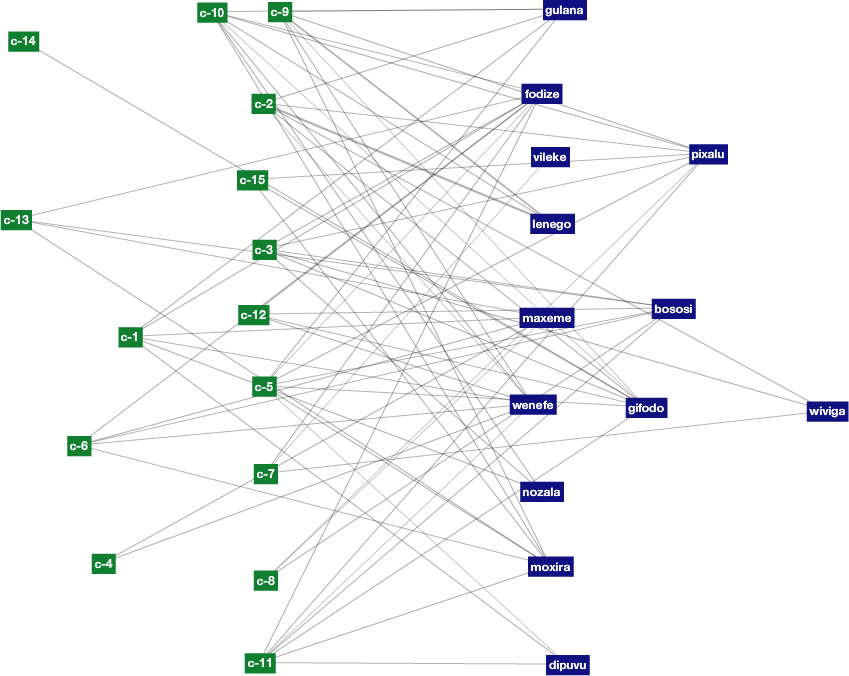
\includegraphics[scale=0.35]{figures/sfwm-lexicon-500} \\
    \\
    \\
    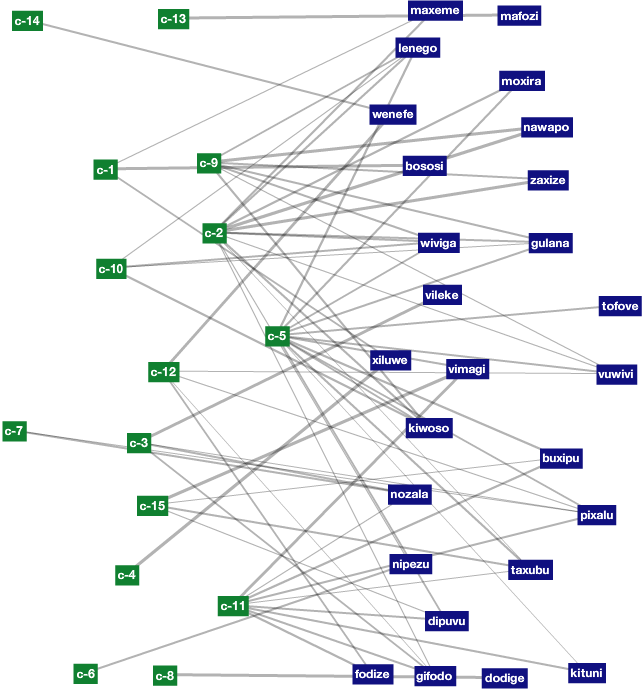
\includegraphics[scale=0.35]{figures/sfwm-lexicon-10000} \\
    \\
  \end{tabular}
  \caption{A network visualization of the lexicon of a single agent at
    interaction 500 (top) and interaction 10000 (bottom). For each
    word denoted by its form, all categories that are associated to
    the form are shown. The line width represents the certainty scores
    of these associations.  }
  \label{f:sfwm-semiotic-network}
\end{figure}

Nevertheless, agents communicate already successfully in the majority
of the shown early interactions. Interestingly (and very different
from the experiments in the previous chapter), agents that use
multiple words in an utterances are more likely to reach their
communicative goal than agents that use only single words. For example
in interaction 502, the speaker uses the three different words
``xamexu'', ``bovaze'' and ``dugobo'', and although the hearer has a
very different understanding what these words mean, the interaction
results in a communicative success. The reason for this is that using
more words doesn't increase the danger of using them in a wrong
``wrong'' way as in the experiments before, but quite to the contrary
adds to the chances of being understood by being more expressive. When
words are not very conventionalized yet but some coherence exists,
then the more words are used, the higher the chance that the overall
similarity to the similarity to objects in the context selects the
correct topic.



\startfiguregroup

\begin{figure}[t]
  
{\footnotesize\renewcommand{\arraystretch}{1.5}
\begin{tabular}{@{}p{1.2cm}|p{1.3cm}@{}p{0.8cm}@{}|p{1.3cm}@{}p{0.8cm}@{}|p{1.3cm}@{}p{0.8cm}@{}|p{1.3cm}@{}p{0.8cm}@{}}
form & agent 1 &  & agent 2 &  & agent 3 &  & agent 4 & \\
\hline
\textit{"sidigu"} & \texttt{c-8}

\texttt{c-6}

\texttt{c-5}

\texttt{c-7}

\texttt{c-3} & 0.34

0.34

0.26

0.17

0.17 & \texttt{c-6}

\texttt{c-8}

\texttt{c-5}

\texttt{c-3}

\texttt{c-4}

\texttt{c-1} & 0.32

0.17

0.17

0.09

0.05

0.04 & \texttt{c-6}

\texttt{c-7}

\texttt{c-3}

\texttt{c-8}

\texttt{c-5} & 0.20

0.20

0.10

0.10

0.10 & \texttt{c-8}

\texttt{c-3}

\texttt{c-5}

\texttt{c-2}

\texttt{c-6} & 0.39

0.32

0.32

0.17

0.09\\
\hline
\textit{"wefugu"} & \texttt{c-8}

\texttt{c-7}

\texttt{c-1}

\texttt{c-2}

\texttt{c-12}

\texttt{c-9}

\texttt{c-5} & 0.30

0.22

0.13

0.02

0.02

0.02

0.02 & \texttt{c-8} & 0.13 & \texttt{c-1}

\texttt{c-2}

\texttt{c-11}

\texttt{c-8}

\texttt{c-7}

\texttt{c-6}

\texttt{c-15}

\texttt{c-4} & 0.13

0.13

0.10

0.10

0.10

0.02

0.02

0.02 & \texttt{c-4}

\texttt{c-7}

\texttt{c-11}

\texttt{c-6} & 0.17

0.17

0.02

0.02\\
\hline
\textit{"vufaxe"} & \texttt{c-5}

\texttt{c-9}

\texttt{c-2}

\texttt{c-12} & 0.43

0.25

0.14

0.08 & \texttt{c-5}

\texttt{c-9}

\texttt{c-12}

\texttt{c-14} & 0.38

0.35

0.20

0.11 & \texttt{c-5}

\texttt{c-9}

\texttt{c-12}

\texttt{c-2} & 0.57

0.40

0.17

0.15 & \texttt{c-9}

\texttt{c-2}

\texttt{c-5}

\texttt{c-12}

\texttt{c-14} & 0.30

0.30

0.14

0.06

0.06\\
\hline
\textit{"bivura"} & \texttt{c-8}

\texttt{c-7}

\texttt{c-1}

\texttt{c-2}

\texttt{c-4}

\texttt{c-5}

\texttt{c-3} & 0.24

0.19

0.17

0.14

0.09

0.06

0.06 & \texttt{c-5}

\texttt{c-9}

\texttt{c-1}

\texttt{c-14}

\texttt{c-12}

\texttt{c-6}

\texttt{c-8}

\texttt{c-7} & 0.31

0.11

0.10

0.10

0.10

0.09

0.06

0.06 & \texttt{c-3}

\texttt{c-7}

\texttt{c-4}

\texttt{c-1}

\texttt{c-8}

\texttt{c-5}

\texttt{c-2} & 0.17

0.17

0.13

0.13

0.07

0.07

0.02 & \texttt{c-7} & 0.20\\
\hline
\textit{"kunite"} & \texttt{c-5}

\texttt{c-6}

\texttt{c-9}

\texttt{c-10}

\texttt{c-2}

\texttt{c-8}

\texttt{c-7}

\texttt{c-3} & 0.13

0.13

0.10

0.10

0.10

0.10

0.02

0.02 & \texttt{c-9}

\texttt{c-5}

\texttt{c-7}

\texttt{c-3}

\texttt{c-4}

\texttt{c-1}

\texttt{c-6}

\texttt{c-2} & 0.10

0.10

0.10

0.10

0.06

0.06

0.06

0.06 & \texttt{c-2}

\texttt{c-4}

\texttt{c-5}

\texttt{c-3}

\texttt{c-1} & 0.20

0.13

0.10

0.10

0.10 & \texttt{c-5}

\texttt{c-1}

\texttt{c-3}

\texttt{c-4}

\texttt{c-2}

\texttt{c-10}

\texttt{c-8} & 0.13

0.10

0.10

0.10

0.10

0.02

0.02
\end{tabular}}

  \caption{Word meanings maintained first four agents of a population
    of 10 for the first 5 forms after 500 interactions. Word
    representations are shown with their association scores to
    different meanings (compared to previous similar charts where
    competing word meanings were shown). }
  \label{f:sfwm-lexicon-forms-500}
\end{figure}

\begin{figure}[t]
  
{\renewcommand{\arraystretch}{1.5}
\begin{tabular}{@{}p{1.2cm}|p{1.3cm}@{}p{0.8cm}@{}|p{1.3cm}@{}p{0.8cm}@{}|p{1.3cm}@{}p{0.8cm}@{}|p{1.3cm}@{}p{0.8cm}@{}}
form & agent 1 &  & agent 2 &  & agent 3 &  & agent 4 & \\
\hline
\textit{"sidigu"} & \texttt{c-8}

\texttt{c-5}

\texttt{c-3}

\texttt{c-6} & 0.68

0.59

0.57

0.48 & \texttt{c-8}

\texttt{c-5}

\texttt{c-3}

\texttt{c-6} & 0.60

0.57

0.55

0.33 & \texttt{c-5}

\texttt{c-8}

\texttt{c-3}

\texttt{c-6} & 0.66

0.63

0.59

0.46 & \texttt{c-8}

\texttt{c-5}

\texttt{c-3}

\texttt{c-6}

\texttt{c-2} & 0.73

0.68

0.50

0.43

0.16\\
\hline
\textit{"wefugu"} & \texttt{c-7}

\texttt{c-8}

\texttt{c-1} & 0.60

0.56

0.21 & \texttt{c-7}

\texttt{c-8}

\texttt{c-4}

\texttt{c-2}

\texttt{c-1} & 0.64

0.51

0.44

0.36

0.32 & \texttt{c-4}

\texttt{c-2}

\texttt{c-8}

\texttt{c-7}

\texttt{c-1} & 0.59

0.46

0.45

0.45

0.26 & \texttt{c-8}

\texttt{c-7}

\texttt{c-4}

\texttt{c-2}

\texttt{c-1} & 0.55

0.53

0.46

0.40

0.13\\
\hline
\textit{"vufaxe"} & \texttt{c-5}

\texttt{c-9} & 0.80

0.44 & \texttt{c-5}

\texttt{c-9}

\texttt{c-12} & 0.77

0.73

0.27 & \texttt{c-5}

\texttt{c-9}

\texttt{c-12} & 0.84

0.67

0.29 & \texttt{c-9}

\texttt{c-5}

\texttt{c-12} & 0.74

0.72

0.22\\
\hline
\textit{"bivura"} & \texttt{c-3}

\texttt{c-5}

\texttt{c-6}

\texttt{c-8}

\texttt{c-7} & 0.53

0.53

0.51

0.38

0.31 & \texttt{c-3}

\texttt{c-7}

\texttt{c-5}

\texttt{c-6}

\texttt{c-8} & 0.70

0.64

0.55

0.54

0.48 & \texttt{c-3}

\texttt{c-5}

\texttt{c-7}

\texttt{c-8}

\texttt{c-6} & 0.67

0.67

0.37

0.32

0.31 & \texttt{c-5}

\texttt{c-3}

\texttt{c-6}

\texttt{c-8}

\texttt{c-7} & 0.61

0.58

0.50

0.36

0.29\\
\hline
\textit{"rotapo"} & \texttt{c-2}

\texttt{c-5} & 0.80

0.53 & \texttt{c-2}

\texttt{c-5} & 0.83

0.54 & \texttt{c-2}

\texttt{c-5}

\texttt{c-3} & 0.86

0.46

0.03 & \texttt{c-2}

\texttt{c-5} & 0.82

0.54
\end{tabular}}

  \caption{Word meanings for the same 4 agents as in Figure
    \ref{f:sfwm-lexicon-forms-500} above, but 4500 interactions later
    (at interaction 5000).}
  \label{f:sfwm-lexicon-forms-5000}
\end{figure}

\stopfiguregroup


\startfiguregroup

\begin{figure}[t]
  \gnuplotfigure{figures/sfwm-attribute-scores-1}
  \caption{Slowly adapting word meanings of a single word of a single
    agent over time. The certainty scores of the associations of the
    form ``lonigo'' to its categories are shown over the course of
    16000 interactions. Not that each agent only takes part in every
    fifth interaction on average. }
  \label{f:sfwm-attribute-scores-1}
\end{figure}

\begin{figure}[t]
  \gnuplotfigure{figures/sfwm-attribute-scores-3}
  \caption{Adapting word meanings of another word over time.}
  \label{f:sfwm-attribute-scores-2}
\end{figure}

\begin{figure}[t]
  \gnuplotfigure{figures/sfwm-attribute-scores-2}
  \caption{Adapting word meanings of yet another word over time.}
  \label{f:sfwm-attribute-scores-3}
\end{figure}

\stopfiguregroup


~\\

\noindent In addition to the flexible lexicon application, the
similarity-based alignment mechanisms are the second key factor for
the dynamics of this lexicon formation model. Instead of deleting
competing hypotheses on word meanings from their lexicons, agents
gradually refine and shift the meanings of their words to better
conform future uses.  Figure \ref{f:sfwm-semiotic-network} shows a
network representation of a single agent's lexicon at interaction 500
and then at interaction 10000. Compared to the similar Figure
\ref{f:sgg-mw-structured-lexicon-500} (page
\pageref{f:sgg-mw-structured-lexicon-500}) from the last chapter for
the same simulated environment, there are much less word forms in the
lexicon after 500 interactions. During the next 9500 interaction, this
agent carefully entrenches his association scores (denoted by the line
widths). Whereas in the beginning words forms are associated to many
categories, words later become more specialized and associate less
categories with higher scores. As a consequence, more words enter the
lexicon as the existing words cover fewer potential meanings. Also
different from the previous competition based dynamics, most of the
word forms from the lexicon at interaction are still around at
interaction 10000.

Analogously, Figures \ref{f:sfwm-lexicon-forms-500} and
\ref{f:sfwm-lexicon-forms-5000} further illustrate the same effects by
showing the categories and association scores for the first 5 forms
for the 4 agents out of a population of 10 agents at 500 and 5000
interactions. Furthermore, Figures
\ref{f:sfwm-attribute-scores-1}--\ref{f:sfwm-attribute-scores-3} show
three typical evolutions of words of a single agent. In Figure
\ref{f:sfwm-attribute-scores-1}, the form ``lonigo'' gets associated
to 8 different categories within the first 4000 interactions. From
very early on, the two categories \texttt{c-1} and \texttt{c-2} become
dominant and from interaction 4000 on, all other categories become
eliminated and the certainty scores for \texttt{c-1} and \texttt{c-2}
continuously increase. For the form ``duropi'' (Figure
\ref{f:sfwm-attribute-scores-2}), it takes a bit longer to find it's
later meaning. After around 3000 interactions, the three categories
\texttt{c-1}, \texttt{c-2} and \texttt{c-4} emerge, of which
\texttt{c-2} has difficulties to become conventionalized and
eventually disappears shortly after interaction 12000. That particular
word is therefore an example of a word that changes its specificity
from being more specific (covering three categories) to more general
(covering two categories). An example for the contrary is the word
``lonigo'' in Figure \ref{f:sfwm-attribute-scores-3}. This one starts
out being very general (covering only the single category
\texttt{c-7}) and later on acquires more meanings (\texttt{c-3} at
interaction 5000 and \texttt{c-2} at interaction 8000), thus becoming
more specific.


\startfiguregroup

\begin{figure}[t]
  \gnuplotfigure{figures/sfwm-success+lexicon-size+coherence}
  \caption{Comm\-unicative success (measure
    \ref{m:communicative-success}), lexicon size (measure
    \ref{m:lexicon-size}) and lexicon coherence (measure
    \ref{m:fwm-lexicon-coherence}) in a population of 10 agents averaged
    over 10 repeated series of 16000 language games. Each measure is
    averaged over the last 250 interactions. }
  \label{f:sfwm-success+lexicon-size+coherence}
\end{figure}


\begin{figure}[t]
  \gnuplotfigure{figures/sfwm-lexicon}
  \caption{The distance of the utterance to the topic (measure
    \ref{m:fwm-distance-utterance-topic}), the average number of
    categories covered per word (measure
    \ref{m:fwm-attributes-per-word}) and the average utterance length
    (measure \ref{m:utterance-length}) are averaged over 10 repeated
    series of 16000 language games}
  \label{f:sfwm-lexicon}
\end{figure}

\stopfiguregroup


\begin{measure}[b]{Lexicon coherence between speaker and
    hearer II}{m:fwm-lexicon-coherence}
  Provides a measure for how similar the lexicons of the interacting
  agents are. After each interaction, the similarity between the
  lexicons of the speaker and the hearer is computed as the average of
  the output of the \texttt{similarity} function for each word form
  that both agents have in their lexicon and of $0$ for all others.

~\\

  Again, the lexicon similarity between speaker and hearer is only an
  approximation of the population coherence, but is used because its
  is much more efficiently computed than a measure that involves
  comparing the lexicons of all agents.
\end{measure}


\begin{measure}[b]{Distance utterance to topic}{m:fwm-distance-utterance-topic}
  Measures how well the words of the utterance cover the topic. After
  each interaction, the average of the \texttt{similarity} function is
  computed between all words used by the speaker and the
  utterance. Results are averaged over the last 250 interactions.
\end{measure}


\begin{measure}[b]{Average number of categories per
    word}{m:fwm-attributes-per-word}
  Measures how specific words are. For all words in an agents lexicon,
  the average number of categories that are associated to a form with
  a non-zero certainty score is computed. Results are averaged over
  all agents of the population and the last 250 interactions.
\end{measure}



~\\

\noindent Finally, the overall alignment dynamics for agents that use
flexible word representations and learning mechanisms are shown in
Figure \ref{f:sfwm-success+lexicon-size+coherence}. Compared to Figure
\ref{f:sgg-mw-structured-success+lexicon-size} on page
\pageref{f:sgg-mw-structured-success+lexicon-size}, two things are
clearly visible. First, agents start communicating successfully from a
bit earlier on but more importantly, never reach 100 percent
communicative success. This is due to the fact that agents often
stretch their existing words in order to apply in difficult contexts
instead of inventing new words, which is interpreted differently by
hearers in about two percent of the cases. Second, the typical
bell-curved evolution of lexicon size does not occur at all. Instead
of inventing and adopting lots of words in the beginning and pruning
them later on, agents grow their lexicons much more
conservatively. Most of the words enter the lexicons in the first few
thousand interactions, but even new words emerge as the lexicons
specialize.

Additionally, Figure \ref{f:sfwm-lexicon} investigates word usage in
more depth. First, the overall distance of the words in the utterance
to the the topic decreases from 1 in the beginning to almost 0.5
(complete category overlap), showing that agents indeed manage to
shape their words to be more applicable in future
conversations. Second, the average number of categories covered per
word decreases from about 5 to a stable level of 3.5 as part of the
entrenchment process. This shows that the word representations are
suitable for maintaining structured word meanings, which was not the
case for the competition based models from the previous chapter
because they contained a frequency-bias towards atomic word meanings.



\section{Robust scaling dynamics}

\startfiguregroup

\begin{figure}[p]
  \gnuplotfigure{figures/sfwm-communicative-success-vs-population-size}
  \caption{Communi\-cative success (measure
    \ref{m:communicative-success}) for five different population
    sizes. Results are averaged over 10 series of varying length, but
    each with 8000 interactions per agent.}
  \label{f:sfwm-communicative-success-vs-population-size}
\end{figure}

\begin{figure}[p]
  \gnuplotfigure{figures/sfwm-lexicon-size-vs-population-size}
  \caption{Lexicon size (measure \ref{m:lexicon-size}) for five
    different population sizes. Results are averaged over 10 series of
    varying length, but each with 8000 interactions per agent.}
  \label{f:sfwm-lexicon-size-vs-population-size}
\end{figure}

\begin{figure}[p]
  \gnuplotfigure{figures/sfwm-lexicon-coherence-vs-population-size}
  \caption{Lexicon coherence (measure \ref{m:fwm-lexicon-coherence})
    for five different population sizes. Results are averaged over 10
    series of varying length, but each with 8000 interactions per
    agent.}
  \label{f:sfwm-lexicon-coherence-vs-population-size}
\end{figure}


\stopfiguregroup

To demonstrate that the lexicon formation model introduced in this
chapter also performs well when the complexity of the interaction
scenario increases, we repeat the scaling studies from the previous
Chapter (see Section \ref{s:sgg-mv-structured-scaling}, page
\pageref{s:sgg-mv-structured-scaling}).

~\\



\startfiguregroup

\begin{figure}[p]
  \gnuplotfigure{figures/sfwm-context-size-vs-communicative-success}
  \caption{Communi\-cative success (measure
    \ref{m:communicative-success}) for world simulators with
    increasing number of objects per scene. Results are averaged over
    10 series of 80000 interactions. }
  \label{f:sfwm-context-size-vs-communicative-success}
\end{figure}


\begin{figure}[p]
  \gnuplotfigure{figures/sfwm-context-size-vs-lexicon-coherence}
  \caption{Lexicon coherence (measure \ref{m:fwm-lexicon-coherence})
    for world simulators with increasing number of objects per
    scene. Results are averaged over 10 series of 80000
    interactions. }
  \label{f:sfwm-context-size-vs-lexicon-coherence}
\end{figure}


\begin{figure}[p]
  \gnuplotfigure{figures/sfwm-context-size-vs-lexicon-size}
  \caption{Lexicon size (measure \ref{m:lexicon-size})
    for world simulators with increasing number of objects per
    scene. Results are averaged over 10 series of 80000
    interactions. }
  \label{f:sfwm-context-size-vs-lexicon-size}
\end{figure}

\stopfiguregroup

\noindent First, Figures
\ref{f:sfwm-communicative-success-vs-population-size}--\ref{f:sfwm-lexicon-coherence-vs-population-size}
present the main alignment dynamics for increasing population sizes of
up to 100 agents. It clearly shows that the model scales well with the
number of agents in the population. Agents communicate successfully
from very early on and high levels of coherence are reached in all
conditions. This is in stark contrast to the same analysis for the
models in the previous chapter (see Figure
\ref{f:sgg-mw-structured-best-best-population-size-vs-communicative-success}),
where agents needed to go through thousands of interactions of random
search without any success whatsoever. Furthermore, the average
lexicon size increases with bigger populations because more words get
independently invented and adapted by the population. Since there is
no explicit mechanism for synonymy damping, these words stay in the
population and specialize on more specific meanings.


A growing number of objects per scene has almost no effect
on the dynamics of the game (see Figures
\ref{f:sfwm-context-size-vs-communicative-success}--\ref{f:sfwm-context-size-vs-lexicon-size}).
This is because more alternative conceptualizations of a scene do not
result in a higher hypothesis space that needs to be explored but
instead only puts a little more burden on the similarity based lexicon
application.

\startfiguregroup

\begin{figure}[t]
  \gnuplotfigure{figures/sfwm-number-of-attributes-vs-communicative-success}
  \caption{Communi\-cative success (measure
    \ref{m:communicative-success}) for world simulators with
    increasing number of available categories. Results are averaged over 10
    series of 80000 interactions. }
  \label{f:sfwm-number-of-attributes-vs-communicative-success}
\end{figure}

\begin{figure}[t]
  \gnuplotfigure{figures/sfwm-number-of-attributes-vs-lexicon-size}
  \caption{Lexicon size (measure \ref{m:lexicon-size}) for world
    simulators with increasing number of available categories. Results
    are averaged over 10 series of 80000 interactions. }
  \label{f:sfwm-number-of-attributes-vs-lexicon-size}
\end{figure}

\begin{figure}[t]
  \gnuplotfigure{figures/sfwm-number-of-attributes-vs-lexicon-coherence}
  \caption{Lexicon coherence (measure \ref{m:fwm-lexicon-coherence})
    for world simulators with increasing number of available
    categories. Results are averaged over 10 series of 80000
    interactions. }
  \label{f:sfwm-number-of-attributes-vs-lexicon-coherence}
\end{figure}

\stopfiguregroup

And finally, Figures
\ref{f:sfwm-number-of-attributes-vs-communicative-success}--\ref{f:sfwm-number-of-attributes-vs-lexicon-coherence}
show what happens when the number of categories in the world
simulation increases. More categories mean that agents invent more
words and thus it takes longer to align their meanings, but
nevertheless the model copes well with an increasing meaning space.




%%% Local Variables: 
%%% mode: latex
%%% TeX-master: "phdbook"
%%% End: 



%% \part{Lexicon formation in embodied agents}
%% 
\setcounter{chapter}{6}

\chapter{Embodiment in humanoid robots}
\label{c:embodiment}


In this third part we will apply the lexicon formation models from the
previous three chapters with to real-world situated interactions of
autonomous robots. We will discuss mechanisms and representations for
conceptualization that allow to link words to the visual perceptions
of the robots and we will analyze what impact the additional
challenges and complexities coming from embodiment and
conceptualization have on the performance of these models. But in
order to do that, we will first dedicate one chapter to the perceptual
and social skills that we endowed the robots with for engaging in
grounded language games\footnote{Some parts of of the first two
  sections of this chapter are taken from \cite*{loetzsch12grounding}
  and additionally appeared in shorter form in
  \cite*{spranger12perceptual}.}.

\begin{figure}[p]
  \begin{tabular}{lr}
    \multicolumn{2}{l}{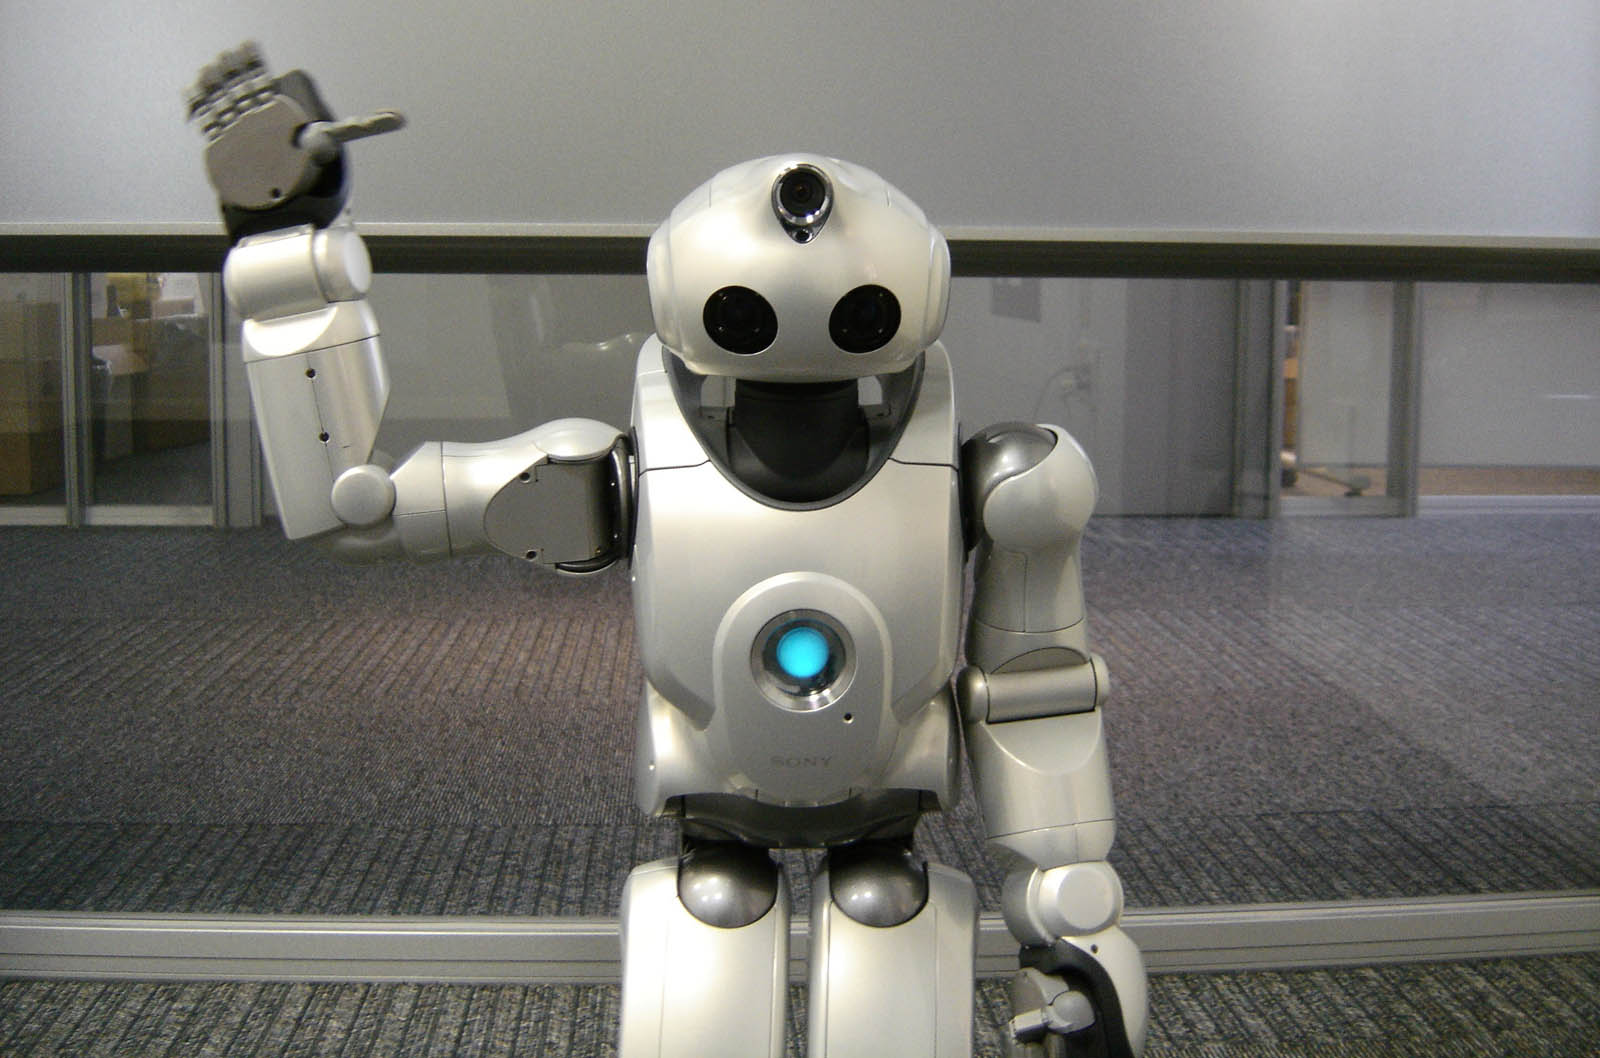
\includegraphics[width=1\textwidth]{figures/photo-qrio-1}} \\
    & \\
    & \\
    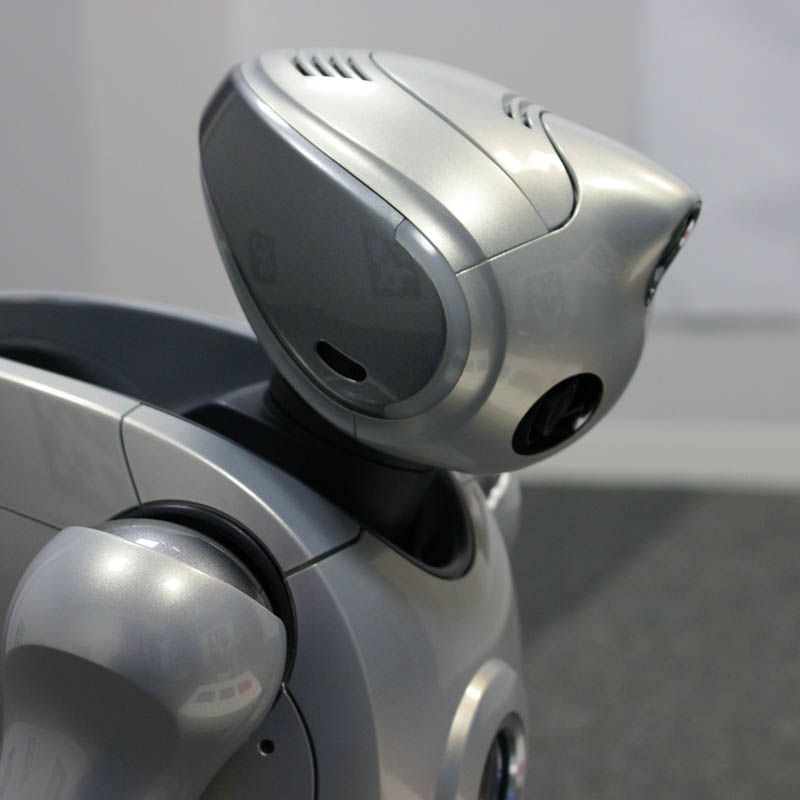
\includegraphics[width=0.48\textwidth]{figures/photo-qrio-3} &
    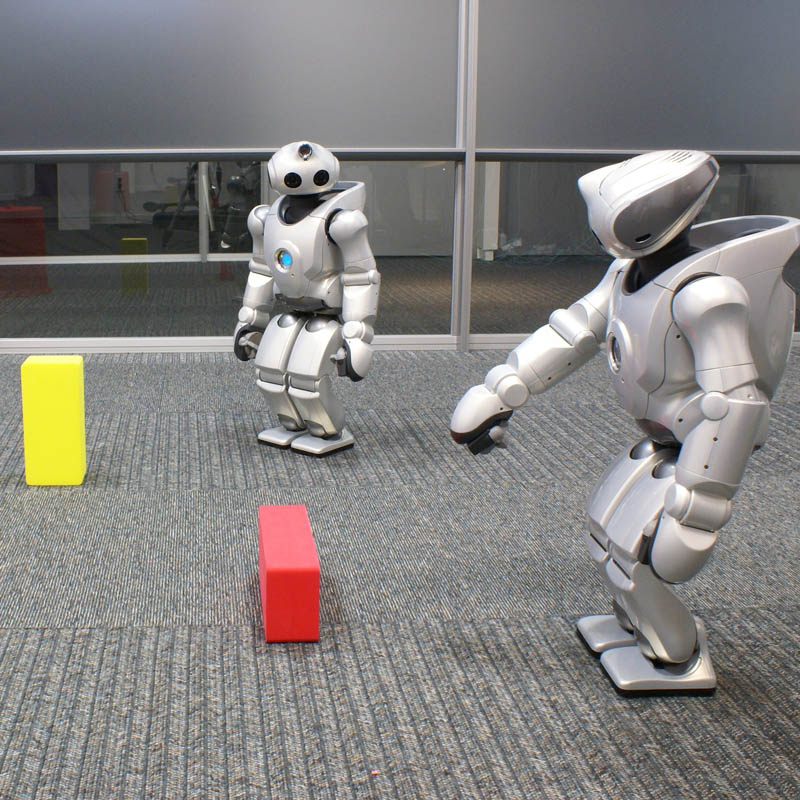
\includegraphics[width=0.48\textwidth]{figures/photo-qrio-2} \\
    & \\
  \end{tabular}
  \caption{The Sony humanoid robot.}
  \label{f:photo-qrio}
\end{figure}


We used two ``Sony humanoid robots'' (\citealp{fujita03autonomous},
see Figure \ref{f:photo-qrio}) for all of our robotic
experiments. They are about 60 cm high, weigh approximately 7 kg and
have 38 degrees of freedom (4 in the head, 2 in the body, 5$\times$2
in the arms, 6$\times$2 in the legs and 5$\times$2 in the
fingers). The main sensors are three CCD cameras in the head, of which
we used here one. The camera delivers up to 30 images per second, has
an opening angle of about 120$^\circ$ and a resolution of
176$\times$144 pixels. It uses the $YCrCb$ color space ($Y$: luma or
brightness, $Cr$: chroma red and $Cb$: chroma blue) with 8 bits per
channel. Furthermore, the robots have three accelerometers and gyro
sensors in the trunk and one accelerometer in each foot. The feet are
equipped with force feedback sensors to detect ground contact. The
batteries have enough capacity for about an hour of autonomous
operation.

We endowed the robots with a vision system for recognizing and
tracking objects in their environment. This system is explained in
Section \ref{s:vision-system} and Section
\ref{s:joint-attention-and-social-skills} introduces a set of social
skills for engaging in language games that were programmed into the
robots. Finally, in Section \ref{s:doing-experiments-with-robots} we
describe the overall experimental setup, i.e. how more high-level
cognitive processess for conceptualization and language interact with
the sensori-motor capabilities of the robots, and we characterize some
properties of the sensory experiences that the robots construct.



\section{Visual object recognition and tracking}
\label{s:vision-system}

\begin{figure}[t]
  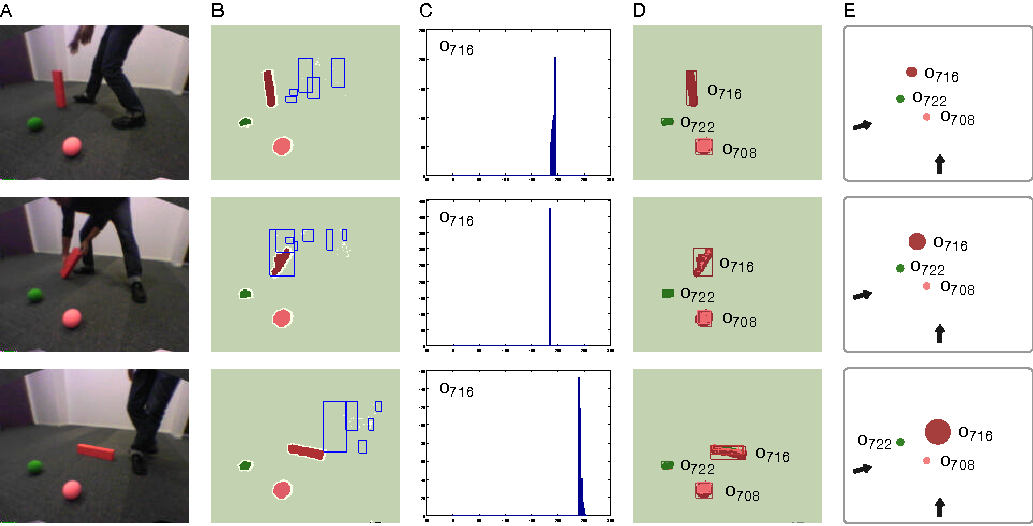
\includegraphics[width=1\textwidth]{figures/vision-system-stages-overview}
  \caption{Image processing steps for three subsequent points in
    time. A: Source images provided by the camera of the robot. B:
    Foreground/ background classification and motion detection (blue
    rectangles). Foreground regions are then associated to existing
    object models or become seeds for new object representations. C/D:
    The changing histogram of the green-red channel for object
    $o_{716}$ is used to track $o_{716}$ in space and time and thus to
    create a persistent model of the object. E: Knowing the offset and
    orientation of the camera relative to the body, the robots are
    able to estimate the position and size of objects in the
    world. Black arrows denote the positions of the two robots
    perceiving the scene.}
\label{f:vision-system-overview}
\end{figure}

The environment of the robots consists of a variety of physical
objects such as toys, cones, barrels and cuboids (see Figure
\ref{f:object-sets}, page \pageref{f:object-sets}) that are initially
unknown to the robots. Objects are frequently added to the scene and
removed again. In addition, objects are moved within a scene and their
appearance may alter. For example the red block in Figure
\ref{f:vision-system-overview}A is standing up in the beginning and is
then put down, changing the perception of the object from being high
and thin to low and broad. In addition, perceiving objects is made
difficult by partial occlusions and other interfering factors such as
human experimenters manipulating the objects in front of the robots.

A prerequisite for building the internal cognitive structures needed
for communicating about objects is that the robots have mechanisms for
constructing perceptual representations of the objects in their
immediate surroundings from the raw sensations streaming from the
robots' sensors. Constructing such representations involves three
sub-systems: First, low-level vision routines process raw camera
images to yield basic \emph{percepts} -- connected regions that differ
from the background of the environment. Figure
\ref{f:vision-system-overview}B gives an example and the mechanisms
involved are explained in Section \ref{s:detecting-foreground-regions}
below. Second, these foreground regions are tracked in subsequent
camera images despite changing positions and appearances of the
objects. In order to do so, the vision system needs to establish a
correspondence between an internal \emph{object model} and the image
regions that refer to the same physical object, a process known in
robotics as \emph{anchoring}
\citep{coradeschi03anchoring,loutfy05maintaining}. For example as
illustrated in Figure \ref{f:vision-system-overview}D, the changing
raw sensations for the red block in Figure
\ref{f:vision-system-overview}A are continously connected to the same
\emph{anchor} $o_{716}$. We used \emph{Kalman Filters} for maintaining
such persistent object models (Section \ref{s:object-models}). Third,
when needed in communicative interactions, the vision system encodes a
set of visual properties about each object model. In this particular
setup these properties are the object's position in a robot egocentric
reference system, an estimated width and height and color information,
as shown in Figure \ref{f:vision-system-overview}E. This process is
discussed further in Section \ref{s:computing-object-features}.


\subsection{Detecting foreground regions in images}
\label{s:detecting-foreground-regions}

The robots do not know in advance what kind of objects to expect in
their environment. Thus, the assumption is made that everything that
was not in the environment before is considered to be a potential
object. The system, therefore, gathers statistical information about 
the environment's background in a calibration phase 
and image regions that sufficiently differ from the background are 
treated as candidates for object models. 
For generating a statistical model of the scene
background, the robots observe the experiment space without objects
for some time (see Figure \ref{f:photo-calibration-phase}) and
perceive a series of calibration images such as in Figure
\ref{f:object-perception}A. For all three color channels $c \in
\{Y,Cr,Cb\}$ the mean $\mu_{c,\vec{p}}$ and variance
$\sigma_{c,\vec{p}}^2$ of the image intensities at every image pixel
$\vec{p}$ are computed over all calibration images. After the
calibration phase the robots are presented with objects, resulting in
raw camera images such as in Figure \ref{f:object-perception}B. The
generated background statistics are used to classify all image pixels
as being foreground or background. A pixel is considered foreground
when the difference between the image intensity $i_c(\vec{p})$ and the
mean of that pixel is bigger than the pixel's standard deviation
($\mid i_c(\vec{p}) - \mu_{c,\vec{p}}\mid > \sigma_{c,\vec{p}}$) for
one of the color channels $c \in \{Y,Cr,Cb\}$. As a result, a binary
image as shown in Figure \ref{f:object-perception}C is generated with
all foreground pixels having the value of $1$ and all others $0$.

\begin{figure}[t]
  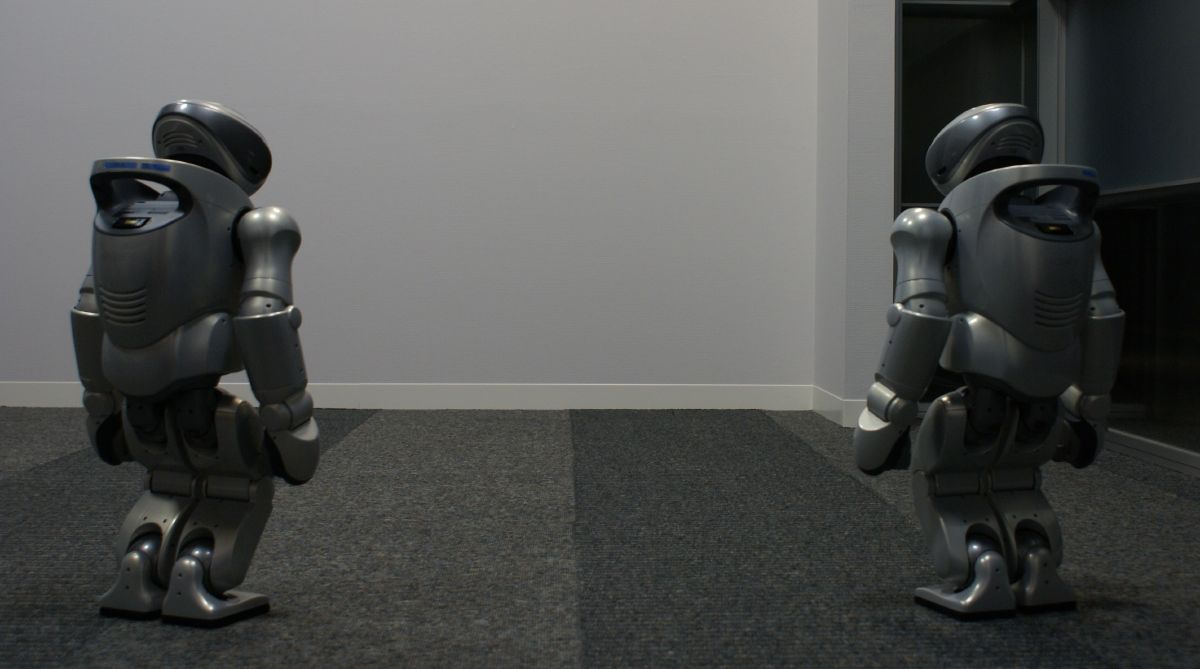
\includegraphics[width=0.65\textwidth]{figures/vision-system-photo-calibration-phase}
  \caption{Calibration phase of the vision system. Both robots are
    shown an empty environment for some extended period of time,
    allowing them to observe the statistical characteristics of the
    scene background.}
  \label{f:photo-calibration-phase}
\end{figure}

\begin{figure}[t]
  \centerline{\footnotesize\sffamily 
    \renewcommand{\arraystretch}{2.0}
    \begin{tabular}{@{}l@{}p{0.025\textwidth}@{}l@{}p{0.025\textwidth}@{}l@{}p{0.025\textwidth}@{}l@{}p{0.025\textwidth}@{}l@{}}
      A & & B & & C & & D \\
      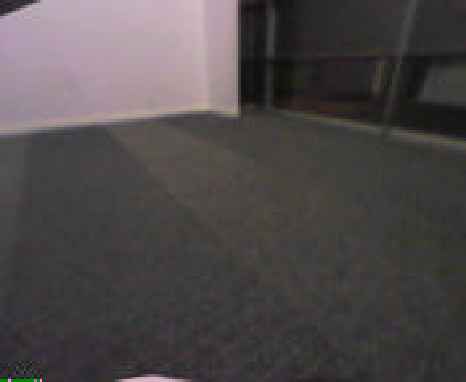
\includegraphics[width=0.23\textwidth]{figures/vision-system-object-perception-1} & &
      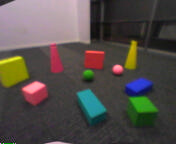
\includegraphics[width=0.23\textwidth]{figures/vision-system-object-perception-2} & &
      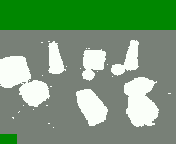
\includegraphics[width=0.23\textwidth]{figures/vision-system-object-perception-3} & &
      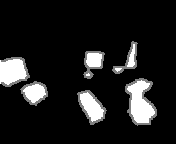
\includegraphics[width=0.23\textwidth]{figures/vision-system-object-perception-4} \\
      E & & F & & G & & H \\
      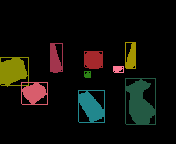
\includegraphics[width=0.23\textwidth]{figures/vision-system-object-perception-5} & &
      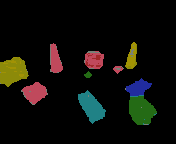
\includegraphics[width=0.23\textwidth]{figures/vision-system-object-perception-6} & &
      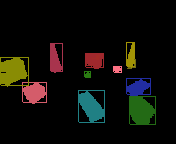
\includegraphics[width=0.23\textwidth]{figures/vision-system-object-perception-7} & &
      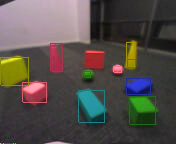
\includegraphics[width=0.23\textwidth]{figures/vision-system-object-perception-8} \\
    \end{tabular}}
  \caption{From foreground regions to object models. A: A raw camera
    image taken during the calibration phase. B: A camera image of a
    scene containing objects. C: The result of foreground/ background
    classification. White pixels are foreground, green pixels were not
    classified. D: The noise-reduced classification image. E: The
    segmented foreground regions drawn in their average color and with
    bounding boxes. Note that the partially overlapping blue and green
    blocks in the right bottom of the original image are segmented
    into the same foreground region. F: Classification of foreground
    pixels using existing color models. Pixels are drawn in the
    average color of the most similar object model. G: Bounding boxes
    and average colors of the segmented classification image. Note
    that the use of previous color models helped to generate separate
    percepts for the blue and green blocks at the right bottom of the
    image. H: Kalman filtered object models. The state bounding boxes
    are drawn in the average color of the model. I: Computation of
    position and size in a robot-egocentric reference system. The
    width and height of objects is indicated by the width and height
    of the triangles.}
  \label{f:object-perception}
\end{figure}

This binary image is further noise-reduced using standard image
operators (dilatation, erosion, see for example
\citealp{parker96algorithms,soille02morphological}) as illustrated in
Figure \ref{f:object-perception}D. First, noise is removed through
applying a $3\times 3$ erosion operator. Second, the change in size of
regions caused by the erosion operator is compensated by applying a
$3\times 3$ dilation operator. Then a segmentation algorithm scans the
filtered image and computes for all connected foreground pixels a
surrounding polygon, the bounding box, and color histograms of the
pixels contained in the region (for each color channel, from the
original image). Color histograms $M^c$ represent frequencies of image
intensities on the color channel $c$, computed either over complete
images or parts of them in the case of foreground regions. The whole
range of intensities is divided into $m$ bins $k~\in~\{1,\dots,m\}$ of
equal size. The number of pixels that have intensities falling into
each bin $M^c(k)$ is counted using a function $h(i_{c}(\vec{p}))$ that
assigns the intensity $i_c$ of a pixel $\vec{p}$ to a bin
$k$. Normalized histograms $\hat{M}^c(k)$ are computed from such
histograms by dividing each frequency $M^c(k)$ by the number of pixels
sampled, resulting in a representation where the sum of all
$\hat{M}^c(k)$ for $k~\in~\{1,\dots,m\}$ is equal to $1$, allowing to
interpret $\hat{M}(h(i_c(\vec{p})))$ as the probability of an image
intensity to occur in an image (or a sub-region). Figure
\ref{f:object-perception}E shows the estimated bounding boxes and
average colors extracted from the regions.



Objects frequently occlude each other, due to particular spatial
placement, but also when moved around in the scene.  For example the
green cube is partly overlapping the blue cuboid in the right bottom
of Figure \ref{f:object-perception}B and thus the segmentation
algorithm creates only one foreground region for both
objects. Provided that there is an established object model (see next
Section \ref{s:object-models}) for at least one of the objects, it is
possible to further divide such regions. Each pixel in a foreground
region is assigned to the most similar color model of previously
perceived objects as shown in Figure \ref{f:object-perception}F. Given
the normalized color histograms $M_I^c$ of all pixels in the current
image $I$ and $M_1^c,\dots,M_n^c$ of the $n$ previously established
object models, the likelihood $p_j$ of a pixel $\vec{p}$ in a
foreground region to belong to a color model $j$ can be calculated:

$$p_{j}(\vec{p})=M^Y_{j}(h(i_Y(\vec{p}))) \cdot M_{j}^{Cr}(h(i_{Cr}(\vec{p}))) \cdot M_{j}^{Cb}(h(i_{Cb}
(\vec{p})))$$

\noindent Based on this probability, each pixel is either classified
to belong to the model $j$ with the highest likelihood
$\operatorname{class}({\vec{p}})=\arg\max_{j=1..n}(p_{i}(\vec{p}))$
or, when the highest $p_{j}$ is smaller than a threshold $t$ or when
no previous model exists, to a ``no model'' class. Classified pixels
are again segmented into connected regions. As shown in Figures
\ref{f:object-perception}G and \ref{f:object-perception}H, the
initially connected foreground region for the blue and green objects
in the right bottom of the image could be divided into separate
regions due to the use of previous color models.


The resulting subdivided foreground regions are called
\emph{percepts}.  They represent the result of the low-level image
processing mechanisms acting separately on each image without
incorporating past knowledge (except for the color information of
previous objects). A percept $P$ is defined as $P:=\langle
x_P,y_P,w_P,h_P,M_P^Y,M_P^{Cr},M_P^{Cb},n_P\rangle$ with $x_P,y_P$
describing the center of the percepts bounding rectangle in image
coordinates, $w_P$ and $h_P$ the width and height of the bounding
rectangle in pixels, $M_P^Y$, $M_P^{Cr}$ and $M_P^{Cb}$ the normalized
histograms for the three color channels and $n_P$ the number of pixels
contained in the region.\\

\noindent In order to improve the tracking algorithm described in the next
Section, we also implemented a component for identifying regions in
the image where motion has occured. Image intensities
$i_{c,t}(\vec{p})$ at time $t$ are compared to those of images taken
at time $t-1$. A pixel $\vec{p}$ is classified as subject of motion
when the difference is bigger than the standard deviation
$\sigma_{c,\vec{p}}$ of this pixel's intensities calculated during the
calibration phase ($\mid i_{c,t}(\vec{p}) - i_{c,t-1}(\vec{p})\mid >
\sigma_{c,\vec{p}}$) for one of the color channels $c
\in\{Y,Cr,Cb\}$. The resulting classification image is noise-reduced
and segmented into regions of motion as shown in Figure
\ref{f:vision-system-overview}B. This information is used to loosen
the parameters for the association of percepts to object models.  If
there is motion in a particular region of the image, then object
models are allowed to move and change color more drastically than if
there is no motion.



\subsection{Maintaining persistent object models}
\label{s:object-models}

For maintaining a set of stable and persistent models of the objects
in their environment, the robots have to associate the percepts
extracted from each raw image to existing object models. Furthermore,
they have to create new models when new objects enter the scene and
eventually delete some models when objects disappear. This task is
difficult because objects can move and the detection of regions
through foreground/background separation is noisy and
unreliable. Extracted properties such as size or position may highly
vary from image to image and it can happen that objects are only
detected in some of the images streaming from the camera.


The internal object model $O_t$ of an object at time step $t$
(whenever a new camera image is processed) is defined as $O_t:=\langle
id_O,s_{O,t},\Sigma_{O,t},M^Y_{O,t},M^{Cr}_{O,t},M^{Cb}_{O,t}\rangle$,
with $id_{O}$ being an unique id serving as an anchor for the object,
$s_{O,t}$ a state vector capturing spatial properties, $\Sigma_{O,t}$
the $8 \times 8$ state covariance matrix and $M_{O,t}^Y$,
$M_{O,t}^{Cr}$ and $M_{O,t}^{Cb}$ normalized color histograms. A state
vector $s$ is defined as $s_{O,t}:=\begin{pmatrix} x_{O,t} & y_{O,t} &
  w_{O,t} & h_{O,t} & \dot{x}_{O,t} & \dot{y}_{O,t} & \dot{w}_{O,t} &
  \dot{h}_{O,t}\end{pmatrix}^T$, with $x_{O,t},y_{O,t}$ describing the
center of the object in the image, $w_{O,t}$ and $h_{O,t}$ the
object's width and the height in pixels and $\dot{x}_{O,t}$,
$\dot{y}_{O,t}$, $\dot{w}_{O,t}$ and $\dot{h}_{O,t}$ the change
variables (speed of change in position and size).

We use Kalman Filters \citep{kalman60new} to model the spatial
component $s_{O,t}$ of object models. In every time step $t$ all Kalman
Filter states $s_{O,t-1}$ and $\Sigma_{O,t-1}$ of the last time step $t-1$
are used to \emph{predict} a new a priori state $\overline{s}_{O,t}$ and a
state covariance matrix $\overline{\Sigma}_{O,t}$ given the $8\times8$
state transition matrix $A$ and the process noise covariance matrix
$Q$:
\begin{eqnarray*}
\overline{s}_{O,t}&:=&As_{O,t-1} \\ 
\overline{\Sigma}_{O,t}&: =& A \Sigma_{O,t-1} A^T+Q
\end{eqnarray*}
We found it sufficient to use a constant state transition matrix $A$,
which predicts every dimension via its change variable
and a constant noise covariance matrix $Q=1^{-5}\cdot I_8$.

Next attempts are made to associate percepts to existing models.
Since the position, dimension and color of objects change over time,
no a priori known invariant properties of objects allow to decide
which percept belongs to which model. Instead, a similarity score
$\hat{s}$ based on position and color is used. The score reflects a
set of assumptions and heuristics, which are based on intuitive
notions of how objects behave, so that experimenters can change the
scene, without having to adjust to particular properties of the vision
system.  First it is assumed that an object can not randomly jump in
the image or disappear at one point in space and appear at
another. Consequently, a spatial similarity $\hat{s}_{euclid}$ can be
defined using the Euclidean distance between the center of a percept
$P$ and the predicted position $\overline{x}_{O,t},\overline{y}_{O,t}$
of a model $O$

$$
\hat{s}_{euclid}(P,O):=1 - \frac{\sqrt{(x_P-\overline{x}_{O,t})^2+(y_P-\overline{y}_{O,t})^2}}{l}
$$

\noindent with $l$ being the length of the image diagonal in
pixels. The result of $\hat{s}_{euclid}$ is $1$ when the two points
are identical and $0$ when they are in opposite corners of the image.
Since objects are assumed to move in a predictable fashion, a
threshold $t_{space}$ restricts the radius around a model in which
percepts are associated -- the spatial association score
$\hat{s}_{space}$ equals to $\hat{s}_{euclid}$ when it is bigger than
$t_{space}$ and $0$ otherwise. Second, it is assumed that objects do
not change their color in a random fashion. An object's color
histogram that has a very high value in a certain bin will not have a
zero value in that bin in the next image. Percepts and object models
can thus be compared using a color similarity $\hat{s}_{color}$. It is
based on the Bhattacharyya coefficient $BC$
\citep{bhattacharyya43measure,aherne98bhattacharyya} that is used as a
similarity measure between two normalized histograms $M$ and $M'$:

$$BC(M,M'):=\sum_{k=1}^{m}\sqrt{M(k) \cdot M'(k)}$$

\noindent Using the color histograms $M_P^c$ of a percept $P$ and the
histograms $M_{O,t-1}^c$ of a previous model $O$, a similarity measure
combining all three color channels is defined as:

$$
\hat{s}_{Bhatt}(P,O) := \prod_{c \in \{Y,Cr,Cb\}} BC(M^c_P,M^c_{O,t-1})
$$

\noindent The association score $\hat{s}_{color}(P,O)$ then yields the
result from the above measure when it is bigger than a threshold
$t_{color}$ or $0$ otherwise. In order to allow more rapid changes in
space and color when objects move, the two association thresholds
$t_{space}$ and $t_{color}$ are loosened when motion has been detected
within the area spawned by a state.

The overall similarity score between a particular percept and an
existing object model is then defined as:

$$\hat{s}(P,O)= \hat{s}_{space}(P,O) \cdot \hat{s}_{color}(P,O)$$

\noindent Each percept is associated with the internal state that has
the highest association non-zero score $\hat{s}$ with respect to that
percept. If no such state exists (when either the spatial or color
similarity is below the threshold), then the percept is stored in a
list of unassociated percepts.

  
\begin{figure}[t]
  \parbox{0.486\textwidth}{%
    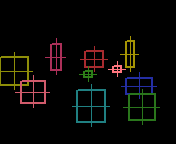
\includegraphics[width=0.23\textwidth]{figures/vision-system-object-modeling-1}%
    \hspace{0.025\textwidth}%
    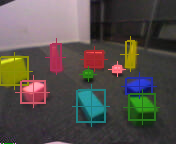
\includegraphics[width=0.23\textwidth]{figures/vision-system-object-modeling-2}}
  \caption{Kalman filtered object models. The state bounding boxes are
    drawn in the average color of the model and the state covariance
    is visualized with the thin cross in the center of each model.}
  \label{f:object-modeling}
\end{figure}

The Kalman Filter states are \emph{updated} given the associated
percepts, which are beforehand combined into a single percept.
Percepts are combined by computing a bounding polygon and a histogram
representing the color frequency in the combined region.  Using the
predicted a priori state vector $\overline{s}_{O,t}$ and state
covariance $\overline{\Sigma}_{O,t}$ as well as the spatial components
$p$ of the combined percept $p:=\begin{pmatrix}x_P&y_P
  &w_P&h_P\end{pmatrix}^T$, the a posteriori state $s_{t}$ and the a
posteriori state covariance matrix $\Sigma_{O,t}$ are computed

\begin{eqnarray*}
  K_{O,t}&=&\overline{\Sigma}_{O,t} H^T H\overline{\Sigma}_{O,t}H^T+R\\
  s_{O,t}&=&\overline{s}_{O,t}+K_{O,t}(p-H\overline{s}_{O,t})\\
  \Sigma_{O,t}&=&(I-K_{O,t}H)\overline{\Sigma}_{t}
\end{eqnarray*}

\noindent with $R$ as the constant $4\times4$ measurement covariance
matrix (with $R=1^{-1}\cdot I_4$) and $H$ a constant $8\times4$ matrix
relating the measurement space and the state space (with $h_{i,j}=1$
for all $i=j$ and $0$ for all others). In principle $H$ and $R$ are
allowed to change over time, but the above estimates resulted in
sufficient tracking performance.  Additionally, the color histograms
of a state $S$ are updated using

$$M^c_{O,t}(k):=(1-\alpha) M^c_{O,t-1}(k)+\alpha M^c_{P}(k)$$

\noindent for all color channels $c\in\{Y,Cr,Cb\}$, all histogram bins
$k\in\{1,\dots,m\}$ and with $\alpha \in [0,1]$ being the influence
of the combined percept.

New object models are created from unassociated percepts. All
unassociated percepts lying in the same foreground region are combined
and used as a seed for a new model which is assigned a new
unique ID.  In order to avoid creating models from percepts generated
for body parts of the experimenter, new models are only created when
no motion was detected. Models that have not been associated
with percepts for some time are deleted. This mainly happens when
objects disappear from the scene and consequently no percepts are
associated with them. As a result of the modeling process, Figure
\ref{f:object-modeling} shows the object models at the time when the
percepts in Figure \ref{f:object-perception} were generated.


\subsection{Computing object features}
\label{s:computing-object-features}

From each object model, a set of features such as color, position and
size are extracted. These feature vectors are called \emph{sensory
  experiences} and are used by the agents to construct the different
conceptual entities needed for engaging in the different kind of
language games introduced in this thesis.

\begin{figure}[t]
  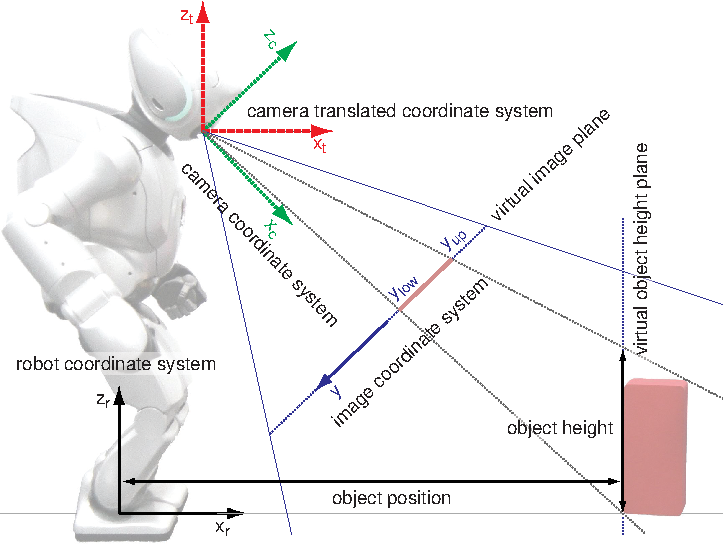
\includegraphics[width=0.75\textwidth]{figures/vision-system-coordinate-systems}
  \caption{Computation of object positions on the ground plane, size
    estimation and the involved coordinate systems. Note that all
    systems except the image coordinate system are three
    dimensional. }
  \label{f:vision-system-coordinate-systems}
\end{figure}


The two robots can perceive the environment from arbitrary angles,
which makes the position and size of objects in the camera image bad
features for communicating about objects. For example the width of an
object in the image depends on how far the object is away from the
robot and is thus not at all shared by the robots. In order to be
independent from how objects are projected onto camera images, spatial
features are computed in an egocentric coordinate system relative to
the robot. However, without the use of stereo vision or a priori known
object sizes, positions can not be determined solely from camera
images. But given the reasonable assumption that objects are located
on the ground, they can be calculated by geometrically projecting
image pixels onto the ground plane using the offset and rotation of
the camera relative to the robot as shown in Figure
\ref{f:vision-system-coordinate-systems}. The egocentric robot
coordinate system originates between the two feet of the robot, the
$z$ axis is perpendicular to the ground and the $x$ axis runs along
the sagittal and the $y$ axis along the coronal plane. First, a
virtual image projection plane orthogonal to the optical axis of the
camera is used to relate image pixels in the two-dimensional image
coordinate system to the three-dimensional camera coordinate system
(which has its origin in the optical center of the camera, with the
$x$ axis running along the optical axis and the $y$ and $z$ an axis
being parallel to the virtual image plane). Given the camera
resolution height and width $r_{w}$ and $r_{h}$ (in pixels) as well as
the horizontal and vertical camera opening angle $\phi_{v}$ and
$\phi_{h}$, the $x_i$ and $y_i$ coordinates of an image pixel can be
transformed into a vector $\vec{v}_c$ in the camera coordinate system

$$
\vec{v}_{c}= \begin{pmatrix}1\\
  -\frac{x_i}{r_{h}} \cdot \tan\frac{\phi_{h}}{2}\\
  \frac{y_i}{r_{v}} \cdot \tan\frac{\phi_{v}}{2}\\
\end{pmatrix}
$$

\noindent that ``points'' to the pixel on the virtual projection
plane. Given the orientation of the camera relative to the robot
represented by the $3\times3$ rotation matrix $R_{c}$, a vector
$\vec{v}_c$ can be rotated into a vector $\vec{v}_t$ in the camera
translated coordinate system (which originates in the center of the
camera, with the axes being parallel to the robot coordinate system)
with $\vec{v}_{t}=R_{c} \cdot \vec{v}_{c}$. Furthermore, given the
offset from the origin of the robot coordinate system to the center of
the camera $\vec{t}_{c}$, the position of a pixel projected onto the
ground plane $\vec{v}_r$ in the egocentric robot coordinate system can
be computed by intersecting the ray $\vec{v}_{t}$ with the ground
plane using simple geometric triangulation: The equation

$$
\vec{v}_r= a \cdot \vec{v}_t + \vec{t}_c
$$

\noindent with the unknown scalar $a$ has exactly one solution for
$x_r$ and $y_r$ when the pixel designated by $\vec{v}_t$ lies below
the horizon.  The operating system of the Sony humanoid readily
provides estimates for $R_{c}$ and $\vec{t}_{c}$ that are computed
from joint sensor values.

Using these transformations, the position features {\tt x} and {\tt y}
(in mm) are extracted from an object model by projecting the pixel at
the center of the lower edge of the object's bounding box onto the
ground plane. For estimating a {\tt width} feature, the lower left and
right corner of a the bounding box are transformed into positions
relative to the robot and the distance between them is calculated. For
the computation of {\tt height}, the ray of the pixel on the middle of
the upper bounding box edge is intersected with a virtual plane
perpendicular to the ground and through the position of the object as
shown in Figure \ref{f:vision-system-coordinate-systems}.  The
extraction of color features from object models is also
straightforward. The feature {\tt luminance} is computed as the mean
of an internal state's color histogram $M_t^{Y}$, {\tt green-red} as
the mean of $M_t^{Cr}$ and {\tt yellow-blue} from
$M_t^{Cb}$. % Similarily, the {\tt stdev-luminance}, {\tt
%   stdev-green-red} and {\tt stdev-yellow-blue} features are the
% standard deviations of the color histograms $M_t^c$ and express how
% uniform the image pixels perceived for an object are.

\begin{figure}[t]
  \parbox{0.75\columnwidth}{%
    \vspace{-3mm}\hspace{3mm}%
    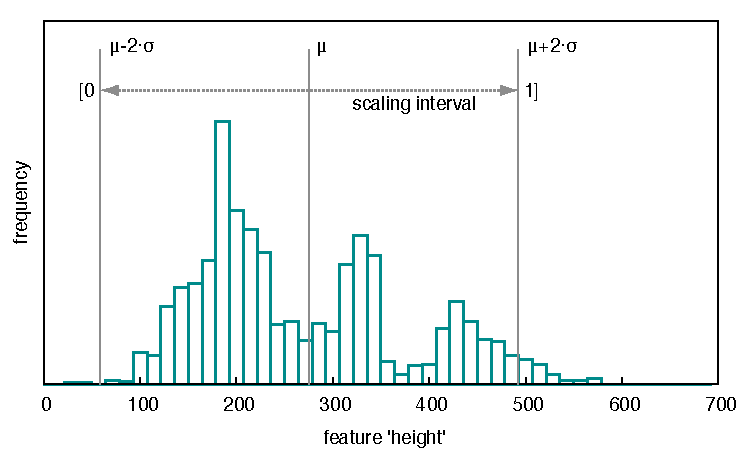
\includegraphics[width=0.75\columnwidth]{figures/vision-system-scaling}}
  \caption{Scaling of feature values. The distribution of the 'height'
    feature sampled over all objects of the geometric objects data set
    (see Section \ref{s:recording-data-sets} on page
    \pageref{s:recording-data-sets}) is used to define an interval
    $\mathsf{[\mu-2\sigma,\mu+2\sigma]}$ for scaling feature values
    into the interval $\mathsf{[0,1]}$.}
  \label{f:vision-system-scaling}
\end{figure}

\begin{figure}[t]
  \parbox{\textwidth}{\fontsize{2.25mm}{2.5mm}\sffamily 
  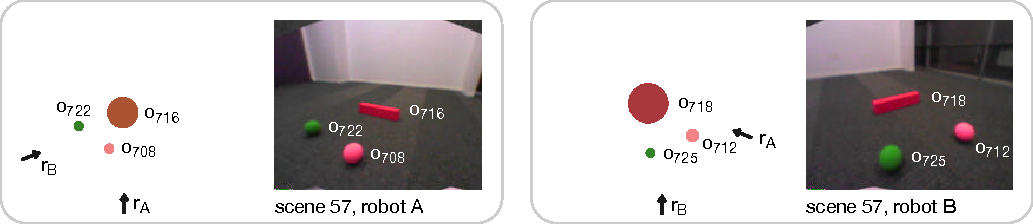
\includegraphics[width=1\textwidth]{figures/vision-system-example-scene}
  \vspace{1mm}
  
  \renewcommand{\arraystretch}{1.5}
  \newcommand{\sub}[1]{\raisebox{-2pt}{\tiny#1}}
  \addtolength{\tabcolsep}{-2.4pt}
  \definecolor{dark}{rgb}{0.5,0.2,0}     
  \hskip0.5mm\begin{tabular*}{\textwidth}{@{}p{17.5mm}|rl|rl|rl||rll|rll|rll@{}}
    & \multicolumn{6}{c||}{experience robot A} & \multicolumn{9}{c}{experience robot B} \\
    feature & 
    \multicolumn{2}{c}{o\sub{708}} & 
    \multicolumn{2}{c}{o\sub{716}} &
    \multicolumn{2}{c||}{o\sub{722}} & 
    \multicolumn{3}{c}{o\sub{712}} & 
    \multicolumn{3}{c}{o\sub{718}} & 
    \multicolumn{3}{c}{o\sub{725}} \\
    \hline
    x & 464 & 0.43 & 821 & 0.69 & 686 & 0.59
    & 607 & 0.53 & \itshape\textcolor{dark}{0.11}
    & 925 & 0.76 & \itshape\textcolor{dark}{0.08}
    & 432 & 0.40 & \itshape\textcolor{dark}{0.19} \\
    y & 151 & 0.61 & 17 & 0.51 & 453 & 0.82
    & -301 & 0.28 & \itshape\textcolor{dark}{0.33}
    & 137 & 0.60 & \itshape\textcolor{dark}{0.09}
    & 115 & 0.58 & \itshape\textcolor{dark}{0.25} \\
    width & 47 & 0.31 & 150 & 1.00 & 46 & 0.30
    & 62 & 0.46 & \itshape\textcolor{dark}{0.15}
    & 196 & 1.00 & \itshape\textcolor{dark}{0.00}
    & 45 & 0.29 & \itshape\textcolor{dark}{0.01} \\
    height & 116 & 0.35 & 138 & 0.42 & 67 & 0.19
    & 109 & 0.33 & \itshape\textcolor{dark}{0.02}
    & 186 & 0.58 & \itshape\textcolor{dark}{0.16}
    & 135 & 0.41 & \itshape\textcolor{dark}{0.22} \\
    luminance & 126 & 0.76 & 72 & 0.30 & 81 & 0.37
    & 130 & 0.79 & \itshape\textcolor{dark}{0.03}
    & 57 & 0.17 & \itshape\textcolor{dark}{0.13}
    & 85 & 0.41 & \itshape\textcolor{dark}{0.03} \\
%     stdev-luminance & 41 & 0.71 & 23 & 0.39 & 22 & 0.36
%     & 39 & 0.69 & \itshape\textcolor{dark}{0.03}
%     & 15 & 0.24 & \itshape\textcolor{dark}{0.15}
%     & 20 & 0.33 & \itshape\textcolor{dark}{0.04} \\
%     min-luminance & 35 & 0.40 & 40 & 0.48 & 29 & 0.31
%     & 26 & 0.26 & \itshape\textcolor{dark}{0.14}
%     & 39 & 0.46 & \itshape\textcolor{dark}{0.02}
%     & 27 & 0.27 & \itshape\textcolor{dark}{0.03} \\
%     max-luminance & 199 & 0.79 & 185 & 0.69 & 126 & 0.30
%     & 198 & 0.78 & \itshape\textcolor{dark}{0.01}
%     & 139 & 0.39 & \itshape\textcolor{dark}{0.30}
%     & 126 & 0.30 & \itshape\textcolor{dark}{0.00} \\
    green-red & 206 & 0.81 & 187 & 0.72 & 101 & 0.29
    & 206 & 0.81 & \itshape\textcolor{dark}{0.00}
    & 196 & 0.76 & \itshape\textcolor{dark}{0.04}
    & 98 & 0.28 & \itshape\textcolor{dark}{0.01} \\
%     stdev-green-red & 17 & 0.71 & 22 & 0.93 & 8 & 0.29
%     & 17 & 0.71 & \itshape\textcolor{dark}{0.00}
%     & 9 & 0.35 & \itshape\textcolor{dark}{0.58}
%     & 8 & 0.30 & \itshape\textcolor{dark}{0.01} \\
%     min-green-red & 149 & 0.76 & 129 & 0.64 & 80 & 0.34
%     & 139 & 0.70 & \itshape\textcolor{dark}{0.06}
%     & 151 & 0.77 & \itshape\textcolor{dark}{0.13}
%     & 76 & 0.31 & \itshape\textcolor{dark}{0.02} \\
%     max-green-red & 233 & 0.79 & 253 & 0.89 & 126 & 0.27
%     & 232 & 0.79 & \itshape\textcolor{dark}{0.00}
%     & 252 & 0.89 & \itshape\textcolor{dark}{0.00}
%     & 123 & 0.26 & \itshape\textcolor{dark}{0.01} \\
    yellow-blue & 119 & 0.53 & 110 & 0.47 & 99 & 0.38
    & 121 & 0.55 & \itshape\textcolor{dark}{0.02}
    & 123 & 0.57 & \itshape\textcolor{dark}{0.10}
    & 97 & 0.37 & \itshape\textcolor{dark}{0.02} \\
%     stdev-yellow-blue & 4 & 0.32 & 22 & 1.00 & 9 & 0.53
%     & 4 & 0.31 & \itshape\textcolor{dark}{0.00}
%     & 4 & 0.29 & \itshape\textcolor{dark}{0.71}
%     & 9 & 0.53 & \itshape\textcolor{dark}{0.00} \\
%     min-yellow-blue & 100 & 0.56 & 39 & 0.12 & 72 & 0.36
%     & 102 & 0.58 & \itshape\textcolor{dark}{0.01}
%     & 95 & 0.53 & \itshape\textcolor{dark}{0.41}
%     & 72 & 0.36 & \itshape\textcolor{dark}{0.00} \\
%     max-yellow-blue & 132 & 0.45 & 133 & 0.46 & 124 & 0.38
%     & 132 & 0.45 & \itshape\textcolor{dark}{0.00}
%     & 140 & 0.52 & \itshape\textcolor{dark}{0.06}
%     & 126 & 0.40 & \itshape\textcolor{dark}{0.02} \\
    \hline
  \end{tabular*}
  \vspace{3mm}
  
}


% (defparameter *world* (make-instance 'physical-robot-world :data-sets '("qrio-1")))
%
% (defparameter *objects* (list (third (entities (get-world-model *world* "scene-3378523360" 'a)))
% 			    (fifth (entities (get-world-model *world* "scene-3378523360" 'a)))
% 			    (fourth (entities (get-world-model *world* "scene-3378523360" 'a)))
% 			    (third (entities (get-world-model *world* "scene-3378523360" 'b)))
% 			    (fifth (entities (get-world-model *world* "scene-3378523360" 'b)))
% 			    (fourth (entities (get-world-model *world* "scene-3378523360" 'b)))))
%
% (loop for i from 0 to 16
%    do (format t "~%      ~(~a~)" (fname (nth i (features (first *objects*)))))
%      (loop for object in (subseq *objects*  0 3)
% 	do (format t " & ~d & ~,2f" (round (value (fvalue (nth i (features object))))) (value (fvalue (nth (+ i 17) (features object))))))
%      (loop for object in (subseq *objects*  3 6)
% 	for j from 3
% 	do (format t "~%      & ~d & ~,2f & \\itshape\\textcolor{dark}{~,2f}" (round (value (fvalue (nth i (features object))))) 
% 		   (value (fvalue (nth (+ i 17) (features object))))
% 		   (abs (- (value (fvalue (nth (+ i 17) (features object)))) (value (fvalue (nth (+ i 17) (features (nth (- j 3) *objects*)))))))))
%      (format t " \\\\"))

%%% Local Variables: 
%%% mode: latex
%%% TeX-master: "../phdbook"
%%% End: 

  \caption{Snapshots of the sensory experiences of both robots at the
    end of the image sequence in Figure
    \ref{f:vision-system-overview}. Top: The camera images at that
    point in time are overlaid with the object anchors maintained by
    the tracking system. Left of them, the positions of objects and
    other robots in the egocentric reference system of each robot are
    shown. Each object is drawn as a circle in its average color, with
    the radius representing the object's width. The positions of the
    two robots (see Section \ref{s:extimating-robot-position} below)
    are indicated using black arrows. Bottom: The actual feature
    values are shown in each first column and feature values scaled to
    the interval $[0,1]$ in each second column.  On the right side of
    the table, the third columns give for each scaled feature the
    difference between the perception of robot A and B.}
  \label{f:vision-system-example-scene}
\end{figure}

The values of the {\tt x} and {\tt y} features are ususally in the
range of meters, {\tt width} and {\tt height} can range from a few
centimeters up to half a meter and values on color channels are within
the interval $[0,255]$. In order to be able to handle all features
independently from the dimensions of their domains, feature values are
scaled to be within the interval $[0,1]$ using the statistical
distributions of feature values as illustrated in Figure
\ref{f:vision-system-scaling} In theory the robots could gradually
build up such distributions by seeing many different objects over the
course of time, in practice the distributions are sampled from objects
of recorded data sets (see Section \ref{s:recording-data-sets}). Given
the mean $\mu$ and standard deviation $\sigma$ of the distribution of
a feature over a (large) number of objects, a scaled value is computed
%$$\overline{v}:=\min(1,\max(0,\frac{v-\mu}{4\cdot\sigma}+\frac{1}{2}))$$
by mapping values in the interval $\mathsf{[\mu-2\sigma,\mu+2\sigma]}$
onto $\mathsf{[0,1]}$ and clipping all others. Figure
\ref{f:vision-system-example-scene} gives an example of the sensory
experiences of the two robots. For each object, both the unscaled and
scaled feature values are given.


\subsection{Visual perception in humans and robots}

The psychological and neurobiological literature on vision contains a
lot of evidence for correlates of these three sub-systems in the human
brain. First, there are dedicated neural assemblies along the visual
stream from the retina to the primary visual cortex that detect basic
visual features on a number of separable dimensions such as color,
orientation, spatial frequency, brightness and direction of movement.
These \emph{early vision} processes operate independently from
attention to objects and features ``are registered early,
automatically, and in parallel across the visual field ''
\citep[p. 98]{treisman80feature-integration}. From there on, two
separate visual pathways (also known as the ``what'' and ``where''
systems) are responsible for identifying objects and encoding
properties about them (see \citealp{mishkin83object} for an early
review): A dorsal stream (the ``where'' system) connecting the primary
visual cortex and the posterior parietal cortex is responsible for the
primitive individuation of visual objects, mainly based on spatial
features. ``Infants divide perceptual arrays into units that move as
connected wholes, that move separately from one another, and that tend
to maintain their size and shape over motion''
(\citealp{spelke90principles}, p. 29). These ``units'' can be
understood as ``pointers'' to sensory data about physical objects that
enable the brain for example to count or grasp objects without having
to encode their properties. They can be compared to the \emph{anchors}
mentioned above and are subject of a large number of studies:
\cite{marr82vision} calls them \emph{place tokens},
\cite{pylyshyn01visual,pylyshyn89role} \emph{visual indexes},
\cite{ballard97deictic} \emph{deictic codes} and
\cite{hurford03neural} discusses them from an artificial intelligence
and linguistics perspective as \emph{deictic variables}. In a second
ventral stream (the ``what'' system) running to the infero-temporal
cortex, properties of objects are \emph{encoded} and temporarily stored in
the \emph{working memory} \citep{baddeley86working-memory} for the use
in other cognitive processes. What these properties are depends on
top-down attentional processes -- for example different aspects of objects
have to be encoded when a subject is asked to count the number of
``big objects'' vs. the number of ``chairs''.


In addition to findings from neuroscience, there is also a variety of
previous work in robotics to rely on. The most widely known setups for
grounding symbolic representations in visual data for the purpose of
communication is probably the Talking Heads experiment
(\citealp{steels98origins}, see \citealp{belpaeme98construction} for
details of the vision system). Static scenes consisting of geometric
shapes on a blackboard are perceived by robotic pan-tilt cameras and
the vision system is able to extract features such as color, size and
position from these shapes. \cite{siskind95grounding} describes a
computer program for creating hierarchical symbolic representations
for simple motion events from simulated video input and in
\citep{siskind01grounding} from real video sequences (see also
\citealp{baillie00action,steels03shared,dominey05learning} for very
similar systems and \citealp{chella00understanding,chella03anchoring}
for a comparable framework inspired by the \emph{conceptual spaces} of
\citealp{gardenfors00conceptual-spaces}).

Furthermore, there is a vast literature on object detection and
tracking algorithms for other purposes than symbol grounding (see
\citealp*{yilmaz06object-tracking} for an extensive review). And the
vision system introduced here does not reinvent the wheel but makes
use of well-established techniques such as color histograms and Kalman
filters. It differs, however, from many other approaches in the notion
of what is considered to be an object. The types of objects that are
expected to occur in the world are often explicitly represented in the
vision system, for example by using pre-specified color ranges for
identifying different object classes in images
(e.g. \citealp{perez02color-based}), by matching (sometimes learnt)
object templates with images (e.g. \citealp{hager98efficient}) or by
engineering dedicated algorithms tailored for recognizing specific
classes of objects (e.g. \citealp*{juengel04real-time}). 

In contrast, our robots have no preconceptions of what to expect in
their environment and thus can detect and track any type of object,
using only two assumptions: First, everything appearing in the
environment that sufficiently distinguishes itself from the background
and that was not there before is considered to be an object. Second,
objects have to be on the ground for being able to make reliable
position and size estimates. Furthermore, what makes the approach
presented here quite special is the tight integration of visual
perception with other cognitive mechanisms such as social behavior
(see below), conceptualization and language (as discussed in the
next chapters).


\section{Joint attention \& mechanisms for social learning in robots}
\label{s:joint-attention-and-social-skills}

Robots learning a language are not only grounded in the physical world
through their sensorimotor apparatus but also socially grounded in
interactions with others. In addition to perceptual capabilities for
detecting and tracking objects in their environment they need a set of
social skills for engaging in communicative interactions with each
other. This includes mechanisms for joint attention and pointing as
well as behavioral scripts for structured conversations. Joint
attentional scenes \citep{tomasello95jointattention} ``are social
interactions in which the child and the adult are jointly attending to
some third thing, and to one another's attention to that third thing,
for some reasonably extended length of time''
\citep[p. 97]{tomasello99cultural}. Establishing joint attention means
in our robotic experiments that two robots taking part in a language
game must (1) share a physical environment, (2) attend to a set of
objects in their surrounding, (3) track whether the respective other
robot is able to attend to the same set of objects and (4) be able to
manipulate attention by pointing to distal objects and perceiving
these pointing gestures (see Figure \ref{f:qrio-pointing}).

\begin{figure}[t]
  \parbox{0.7\textwidth}{ 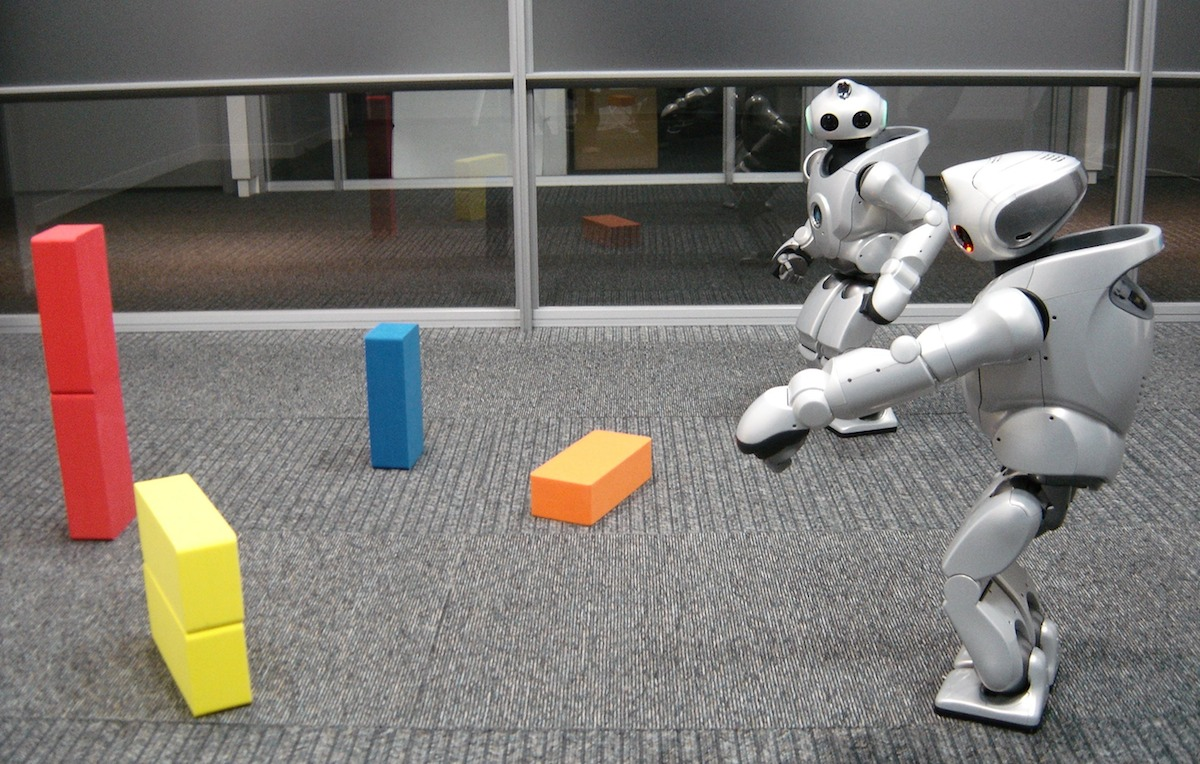
\includegraphics[width=0.7\textwidth]{figures/qrio-pointing-photo-of-scene}
    
    \vspace{0.03\textwidth}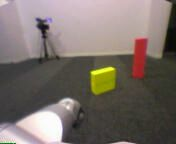
\includegraphics[width=0.335\textwidth]{figures/qrio-pointing-camera-image-b}\hspace{0.03\textwidth}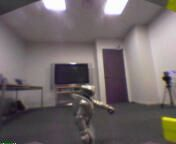
\includegraphics[width=0.335\textwidth]{figures/qrio-pointing-camera-image-a}
  }
  \caption{Demonstration of a Sony humanoid robot drawing the
    attention of the other robot to an object in the shared
    environment by pointing at it. The images at the right show the
    scene as seen through the camera of the pointer (top) and the
    robot observing the pointing (bottom). However, please note that
    the robots are not able to detect pointing gestures using their
    built-in cameras. Instead, they directly transmit $x,y$
    coordinates of the object pointed at.}
  \label{f:qrio-pointing}
\end{figure}

\subsection{Social robotics}

How social mechanisms can be implemented in robots is a research area
in its own. Scientist in this field are mainly interested in how
social skills can improve communication and collaboration between
humans and robots \citep{breazeal02designing}. Additionally, by trying
to endow robots with social behaviors that appear ``natural'' to human
observers, they want to understand what social cues humans are
responding to. For reviews, refer to \cite*{dautenhahn02from} who
developed taxonomies for different degrees of robots' embodiment and
``social embeddedness'', \cite*{fong03survey} who give a general
survey of socially interactive robots, and \cite{vinciarelli09social}
who review the field of ``social signal processing'', i.e. the
detection of social cues in human behavior.  For an overview of skills
that are prerequisites for joint attention and the state of the art in
robotic experiments trying to implement these skills, refer to
\cite{kaplan06challenges}. Some examples of work relevant for the
experiments in this paper are listed below.

\cite{scassellati99imitation} endowed the ``Cog'' robot
\citep{brooks99cog} with capabilities for finding human faces,
extracting the location of the eye within the face, and determining if
the eye is looking at the robot for maintaining eye contact (or mutual
gaze). \cite*{marjanovic99self-taught} showed how the same robot could
learn to control his arm for pointing at distal objects in the
surrounding space, guided by the camera of the robot.  Gaze
recognition was investigated among many others by
\cite{kozima01robot}. They demonstrated how the ``Infanoid'' robot is
able to track gaze direction in human faces and use this information
to identify objects that humans are looking at. Joint attention is
established by alternatingly looking at distal objects and the
faces. \cite{nagai03constructive} modeled the transitions between
different developmental stages that infants are going through in the
process of learning to engage in joint attentional scenes, resulting
in the robot being able to determine which object a human caregiver is
looking at.


For recognizing pointing gestures performed by humans,
\cite*{kortenkamp96recognizing} developed a robot that can detect and
track the 3D positions of arm and shoulder joints of humans in dynamic
scenes, without requiring the humans to wear special markers. By
searching along the vector defined by the detected arm joints, the
robot can determine which object the experimenter was pointing
at. Similarly, \cite{martin09estimation} used pointing gestures to
instruct a mobile robot where to navigate to. \cite*{colombo03visual}
used multiple cameras for tracking humans pointing at areas on walls
in a room.  \cite{nickel07visual} equipped a robot with stereo cameras
and use color and disparity information and Hidden Markov Models to
track both the direction of gaze and the position where a human is
pointing at.  \cite{haasch05multi-modal} apply the ability to
recognize pointing gestures for teaching words for objects in a
domestic environment and \cite*{imai03physical} showed how the robot
"Robovie" could combine mechanisms for establishing mutual gaze and
pointing at objects to draw the attention of humans to a poster in the
environment of the robot. Finally, \cite{hafner05learning}
demonstrated how recognition of pointing gestures could be learned in
Aibo robots. One robot performs a hard-wired pointing gesture and the
other one has to detect whether it was to the left or to the right.

Additionally there is considerable research into implementing and
learning the necessary behaviors for engaging in structured
conversations.  \cite{breazeal03sociable} investigated turn taking
with the Kismet robot, focussing on the factors regulating the
exchange of speaking turns so that the communication seems natural to
human interlocutors.  \cite{cassell99turntaking} discussed how
nonverbal gestures and gaze can support turn taking behaviors in
multimodal dialogs with the embodied conversational agent (ECA)
``Gandalf'', trying to replicate findings from psychologic data. A bit
more on the theoretical side, \cite{iizuka03adaptive} followed a
Dynamic Systems approach for understanding processes of cognition and
action \citep{thelen94dynamic} to understand turn-taking in wheeled
mobile robots in terms of the underlying dynamics of recurrent neural
networks. Recent work on communication with ECAs is reviewed by
\cite{kroeger09model} for the co-ordination of communicative bodily
actions across different modalities and by \cite{kopp10social} for the
alignment of communicative behaviors between interlocutors.



\subsection{Implementing language games in robots}
\label{s:scaffolding-social-skills}

Language games are coordinated by behavioral scripts (see Section
\ref{s:language-game}, page \pageref{s:language-game}). Every agent in
the population knows the language game script and individually reacts
to changes in the environment and actions of the other robot. For
example the speaker triggers the action of pointing to the intended
topic when the hearer signals that he did not understand the
utterance. The scripts are implemented in the form of finite-state
machines: actions are performed depending on the current state in the
game flow, the perception of the environment and the history of the
interaction (see also \citealp*{loetzsch06xabsl}).

Joint attention is monitored by an external computer program, that has
access to the world models of both interacting robots.  This system
initiates the interaction between two agents as soon as both agents
observe the same set of objects.  It is the task of the human
experimenter to find spatial setups in which joint attention is
possible, the program only monitors whether robots are seeing the same
set of objects. But in the literature there are also other proposals
for establishing joint attention in embodied language game
experiments. For example \cite{steels97grounding} programmed
sophisticated signaling protocols into LEGO robots. A robot that
decides to become a speaker emits an infrared signal and the other
robot then aligns its position so that it faces the speaker. The
robots ``point'' to objects by orienting themselves toward them. In
the Talking Heads experiment \citep{steels98origins}, the speaker
directly controls the view direction of the hearer's camera in order
to make sure that their cameras perceive the same objects on the
whiteboard. An agent points to an object by letting the other agent's
camera zoom in on it. In contrast, establishing joint attention in
social language learning scenarios between humans and robots is
usually easier because the human experimenter (as a well-trained
social being) is good at monitoring the attention of the robot and can
for example (as in \citealp{dominey05learning}) point to an object by
moving it.


For constructing a naming system robots need non-linguistic means of
conveying information, such as pointing to an object or conveying
notions of success, failure and agreement in communication.  For
demonstration purposes robots were equipped with behaviors for
pointing at objects (see Figure \ref{f:qrio-pointing}). We used motion
teaching for creating a set of 18 pointing motions for different areas
in front of the robot. Depending on the $x,y$ coordinate of the object
to point at, the pointing routines selects and performs one of these
pre-taught motions. 

Nevertheless, in the communicative interactions underlying the
experiments presented here, robots use a different mechanism in order
to avoid further difficulties stemming from uncertainties in pointing
(see \citealp{steels98stochasticity} for a disscussion of the impact
of such uncertainties on the performance in language games). When a
robot wants to point to an object in the environment, he directly
transmits the $x_o,y_o$ coordinates of the intended object $o$ to the
interlocutor.  Since robots model object positions in their own
(egocentric) coordinate systems, additional steps have to be taken to
interpret these coordinates.  Most importantly the robot has to know
the position $x_r,y_r$ and orientation $\theta_r$ of the robot that is
pointing $r$ (see next Section \ref{s:extimating-robot-position} for
details on how robots estimate these values).  With this information
robots transform the coordinates into their own coordinate system:

$$
\vec{v}=\begin{pmatrix} \cos \theta_r & -\sin \theta_r \\ \sin
  \theta_r & \cos \theta_r \end{pmatrix} \begin{pmatrix} x_o \\
  y_o\end{pmatrix} + \begin{pmatrix} x_r \\ y_r\end{pmatrix}
$$

\noindent The robot interpreting the pointing is determining the
intended object by choosing the object in his world model that is
closest to $\vec{v}$. Furthermore, although we implemented gestures
for giving non-linguistic communicative feedback (nodding the head for
success and shaking for failure) and we used the built-in speech
synthesizer of the Sony humanoid robots for producing utterances,
feedback signals whose meaning is shared and utterances are directly
passed between
interlocutors.\\

\noindent The mechanisms presented in this Section provide simple solutions to
required capacities for social language learning that are not meant to
be in themselves proposals as to how these skills could be
implemented. Nevertheless, we claim that the realism of this study
does not suffer from this simplicity: humans rely on extremely
powerful mechanisms for perceiving and sharing intentions within
interactive situations \citep{tomasello05understanding} and similarly
our solutions provide us with the technical prerequisites for letting
our robots learn from communicative interactions.



\subsection{Robot pose estimation}
\label{s:extimating-robot-position}

A requirement for the pointing mechanisms described above is a quite
precise estimate of the position and orientation of the other
robot. For that, robots localize themselves with respect to landmark
objects in the environment and transmit their position with respect to
these landmarks to the other robot. This way both agents establish
mutual knowledge about their position. We use carton boxes enhanced
with visual markers (see Figure \ref{f:artoolkit}) as landmark
objects.  The unique, black and white, barcode-like, 2D-patterns
attached to carton boxes are tracked using the ARToolKitPlus library
\citep{wagner07artoolkitplus}, which is an improved version of
ARToolKit \citep{kato99marker,kato00virtual}, especially adapted for
mobile devices.

\begin{figure}[t]
  \begin{tabular}{lr}
    \multicolumn{2}{l}{
      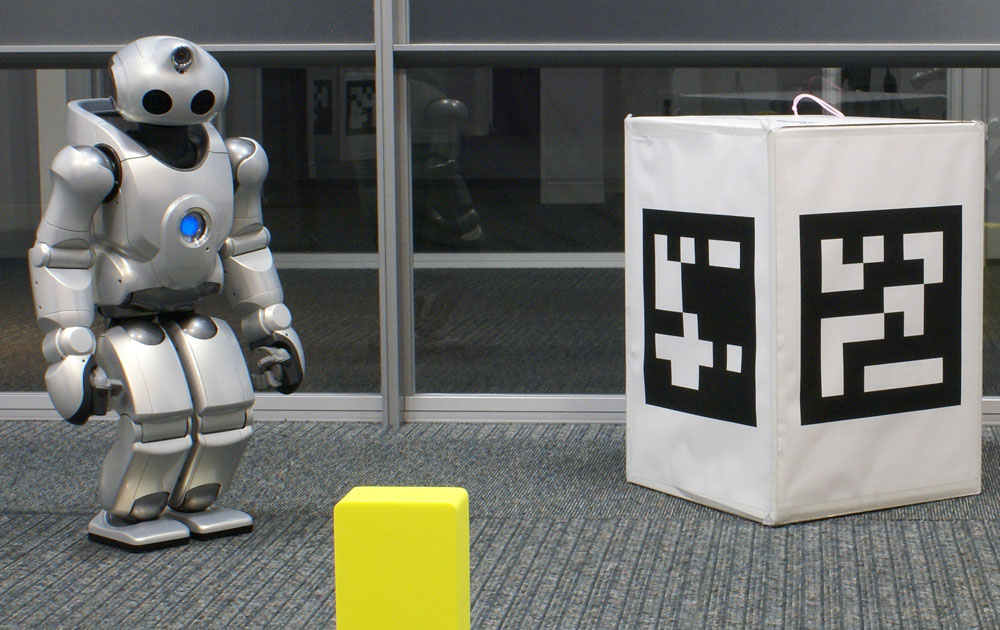
\includegraphics[width=0.6\columnwidth]{figures/artoolkit-0}\vspace{4mm}} \\
    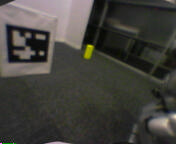
\includegraphics[width=0.28\columnwidth]{figures/artoolkit-1} & 
    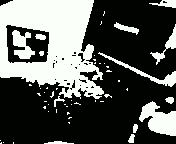
\includegraphics[width=0.28\columnwidth]{figures/artoolkit-2}\vspace{4mm}\\
    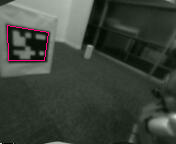
\includegraphics[width=0.28\columnwidth]{figures/artoolkit-3} & 
    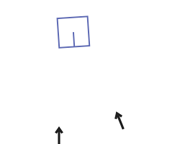
\includegraphics[width=0.28\columnwidth]{figures/artoolkit-4}\\
  \end{tabular}
  \caption{Using objects enhanced with visual markers for estimating
    the position and orientation of the other robot. Top: Example of a
    carton box that is enhanced with 2D patterns. Center left: A
    carton box with markers as seen through the camera of a Sony
    humanoid robot. Center right: Binary image generated from the
    original image.  Bottom left: The marker as detected by the
    ARToolKit tracking system. Bottom right: Both robots send the
    position and orientation of the carton box (blue) to each other
    and are thus able to deduce the position and orientation of the
    respective other robot. }
  \label{f:artoolkit}
\end{figure}

From each camera image, a histogram of the pixel luminance is
computed. This histogram is then used to derive a threshold for
creating a binary image as shown in the top right of Fig.
\ref{f:artoolkit}. The binary image is passed to the tracking library,
which searches it for marker patterns and determines the four vertices
of the polygon surrounding the marker in the image (see bottom left of
Fig. \ref{f:artoolkit}). Provided with the camera resolution width
and height (in pixels), the width and height camera opening angle (in
deg) and the widths of the markers used on the carton boxes (in mm),
the tracking library is able to make an orientation and position
estimate from the edges of the detected patterns, which is then
iteratively enhanced by matrix fitting. As a result, the system
returns for each detected marker pattern a unique ID and a matrix
describing the position and orientation of the marker relative to the
camera of the robot (for details of the pose estimation algorithm
see \citealt*{kato99marker}).

To transform the camera relative marker position and orientation into
robot egocentric coordinates, they are transformed using the offset
and orientation of the camera relative to the ground point of the
robot (see Section \ref{s:computing-object-features}).  Finally, for
each marker attached to a carton box, the offset and orientation
relative to the center of the box, which is a priori known, is used to
determine the position and orientation of the box in egocentric
coordinates. To filter out noise and recognition errors, the resulting
box poses are averaged over the last $n$ images. Also, when two
markers of the same box are detected in the same image, their
resulting box poses are averaged.  The output of the landmark modeling
system is a list of objects consisting of an ID (an ID of the box, not
to confuse with the ID of the marker patterns) and a pose
$\vec{b}:=\begin{pmatrix}x_b & y_b & \theta_b\end{pmatrix}$ of the
carton box in robot egocentric coordinates.


In order to determine the position $x_r,y_r$ and orientation
$\theta_r$ of the respective other robot, the robots use the carton
boxes as global landmarks (see bottom right of Fig.
\ref{f:artoolkit}). About five times per second they exchange the
poses of the boxes they have seen over a wireless network
connection. Given that both robots see the same box (all robots use
the same box IDs for the same visual markers), they can compute the
pose of the other robot from the box pose $\vec{b}$ as perceived by
the robot (in egocentric coordinates) and the $\vec{b}'$ as sent by
the other robot (in the coordinate system of the other robot):

$$
\begin{pmatrix} x_r \\ y_r \\ \theta_r \end{pmatrix} 
:= 
\begin{pmatrix} 
x_b - \cos(\theta_b - \theta_b') \cdot x_b' + \sin(\theta_b - \theta_b') \cdot y_b'  \\
y_b - \cos(\theta_b - \theta_b') \cdot x_b' + \sin(\theta_b - \theta_b') \cdot x_b'  \\
\theta_b - \theta_b'
\end{pmatrix}
$$

\noindent When both robots see multiple boxes the results of the above
transformation are averaged.



\section{Experimental setup}
\label{s:doing-experiments-with-robots}

Integrating all the mechanisms for visual perception and behavior
control into a complete setup for doing language game experiments is a
challenging but also interesting task in its own (see
\citealp{thorisson07integrated} for a discussion of ``integrated
A.I. systems''). It requires computational infrastructure for
connecting single components into a fast and robust system and proper
modularization is needed in order to be able to develop and test
algorithms and behaviors separately. Furthermore, for understanding
the complex dynamics of the experimental setup and for detecting
problems or errors, it is crucial to have visualizations for each
single step in the information processing. Finally, in order to be
able to do repeatable experiments and for testing components without
actually working on a real robot, mechanisms for recording and
replaying each intermediate result of the system are a necessity.

\subsection{Computational infrastructure}

\begin{figure}[t]
  \parbox{\textwidth}{
  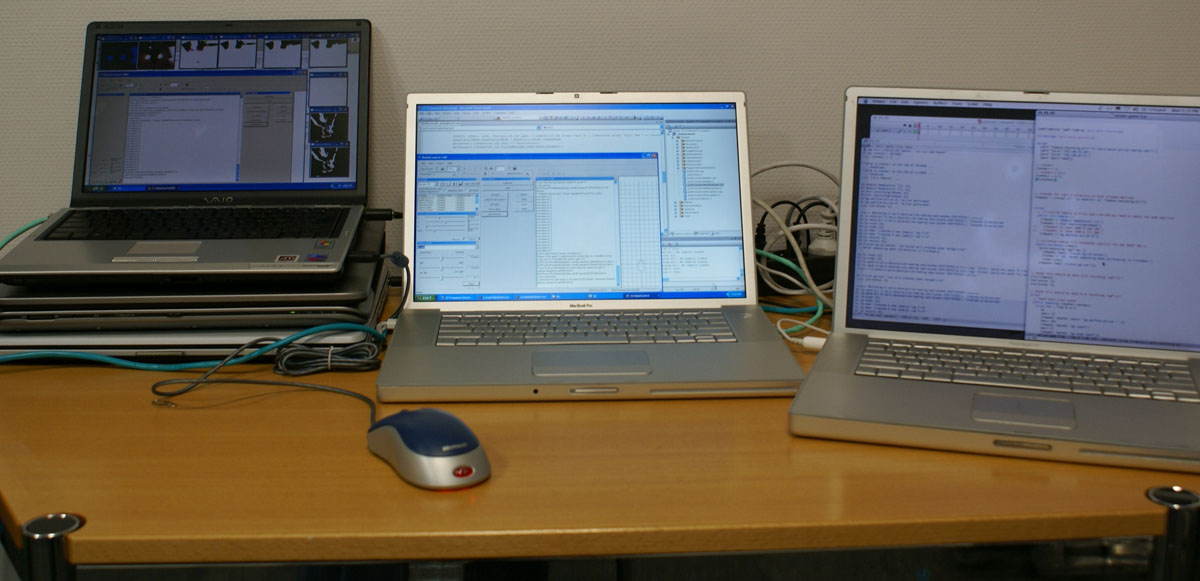
\includegraphics[width=0.48\textwidth]{figures/computer-infrastructure-1}%
  \hspace{0.04\textwidth}%
  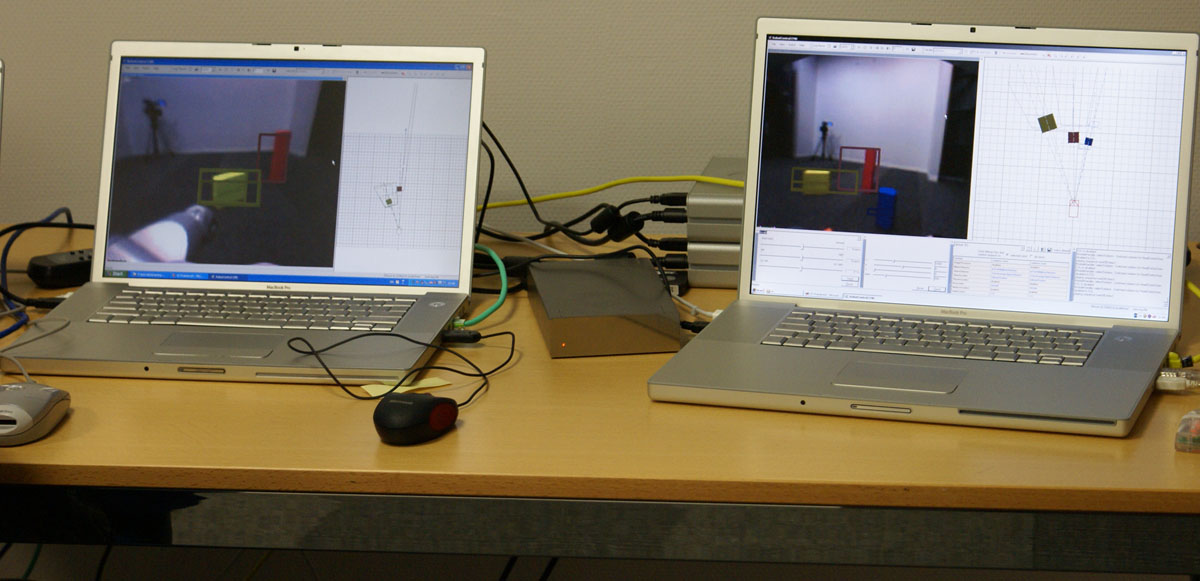
\includegraphics[width=0.48\textwidth]{figures/computer-infrastructure-2}%
  \vspace{0.04\textwidth}
  
  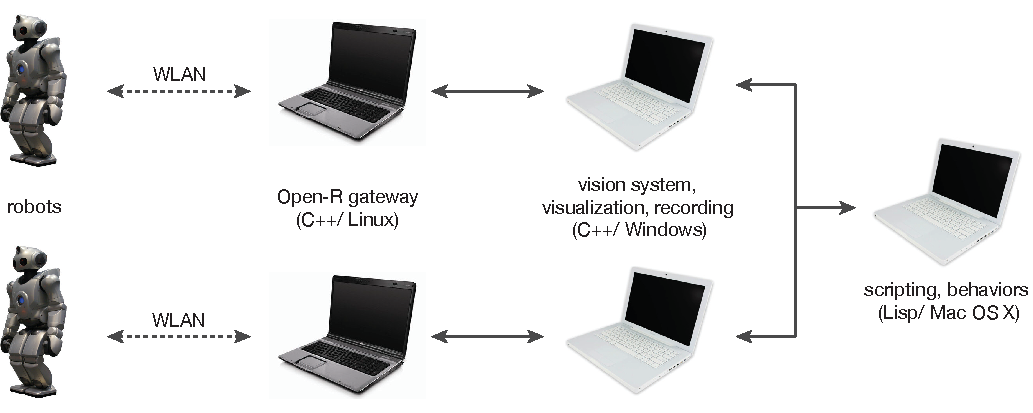
\includegraphics[width=1\textwidth]{figures/computer-infrastructure-network}%
  \vspace{3mm}}
\caption{Computational infrastructure. Top left: five computers were
  involved in conducting the experiments. Top right: real-time
  visualizations of the vision system. Bottom: schematic view of the
  connections between the different subsystems. The robots communicate
  with gateway computers over a wireless network and the computers are
  connected trough an Ethernet network.}
  \label{f:computational-infrastructure}
\end{figure}

The components of the experimental setup are distributed over five
different machines (see Figure \ref{f:computational-infrastructure}),
which is mainly due to the fact that the software involved was written
for different operating systems. The vision system runs in real-time
on an external Microsoft Windows PC (one for each robot). It was
developed on the basis of the 2004 version of the framework used by
the GermanTeam \citep{roefer04germanteam} for participating in the
RoboCup \citep{kitano97robocup} Sony Four Legged League. The
GermanTeam's framework is written in C++ and consists of an
architecture for modularizing tasks, mechanisms for exchanging data
across processes and platforms and a set of powerful debugging
mechanisms \citep{roefer03architecture}.  Besides that, the framework
contains the program \emph{RobotControl}, an application for
visualizing nearly every aspect of the vision system (see top right
image of Figure \ref{f:computational-infrastructure}) and for
debugging and testing components. RobotControl is also used for
recording data to external hard drives and it translates requests from
the language game system (see below) into representations that are
used by the robotic software.

The software running on the Sony humanoid robots was provided by the
members of the Sony Intelligent Systems Research Labs and we used it
without modification. Running on top of the Aperios operating system,
Open-R \citep{fujita97open,ishida01motion} is responsible for
collecting data from sensors and controlling actuators. There are
high-level behavioral primitives for issuing walking commands, gazing
at points in space, performing arm movements, speech output and
more. In the background the system constantly monitors the body
stability and tries to balance walking and other motions, as described
in \citep{nagasaka04integrated}. Furthermore, there is a security
system that triggers a save body posture when the robot is falling.


The communication between the Sony humanoid robots and the
RobotControl program is mediated by a gateway software running on
separate Linux computers. This mediator exchanges data with the robot
using Open-R inter-process communication over a wireless network and
with the Windows software over an Ethernet connection. It translates
images and other sensor data coming from the robot into the
representations used in the GermanTeam's framework and converts
behavior commands coming from RobotControl into data structures
understood by Open-R. Finally, Lisp programs based on the Babel
framework
\citep{loetzsch08babel2,loetzsch09understanding,steels10babel,loetzsch12tools}
and running on a Macintosh computer under Mac OS X were responsible
for central control of the experiments. There are scripts for
coordinating the behaviors of the two robots, for organizing the
recording of data and for provinding the language game framework with
the world models constructed by the robots' vision systems.

\begin{figure}[t]
  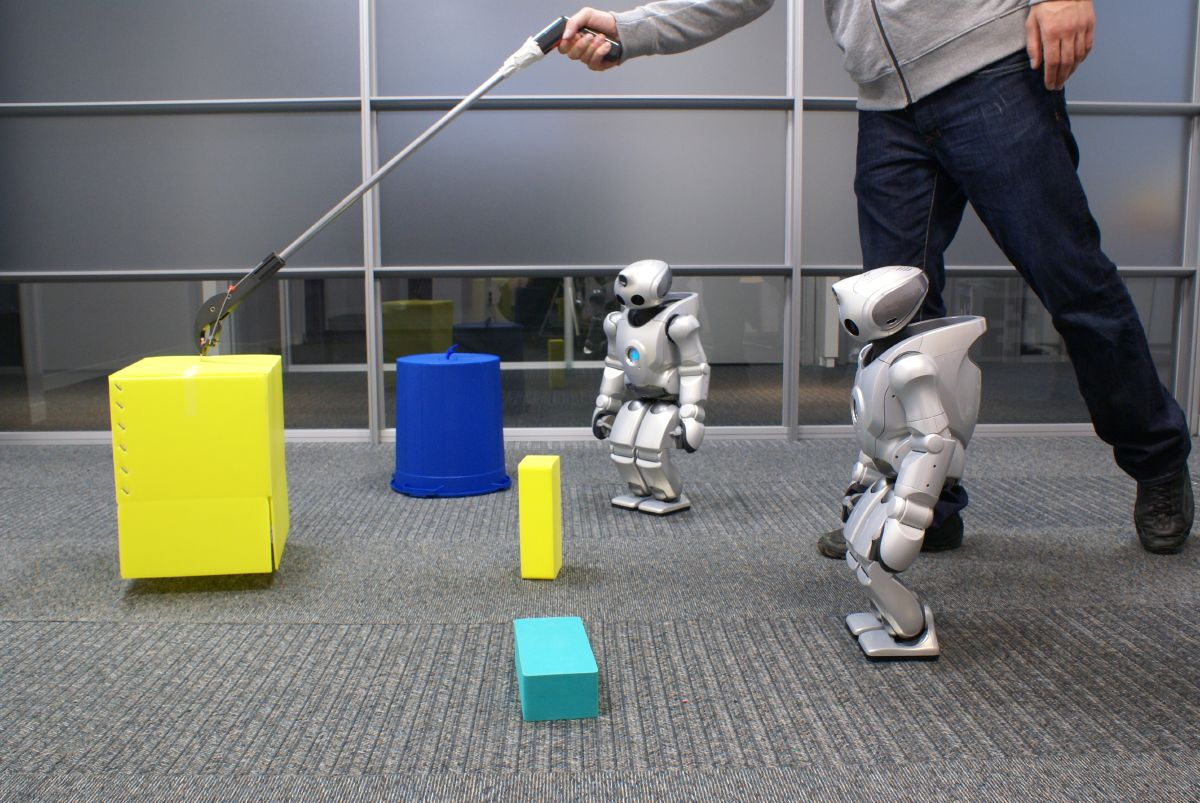
\includegraphics[width=0.48\textwidth]{figures/data-sets-recording-moving-objects}%
  \hspace{0.04\textwidth}%
  \includegraphics[width=0.48\textwidth]{figures/data-sets-recording-screen}
  \caption{Recording data sets. Left: a human experimenter
    systematically adds objects to or removes them from the space
    infront of the robot. Right: in order to make sure that all objects
    occur together with equal distribution in the recorded data set, a
    computer program running on an external computer instructs the human
    experimenter how to modify the scene.}
  \label{f:recording-data-sets}
\end{figure}

~\\

In our embodied language game experiments, agents play tens of
thousands of language games to reach communicative success and
coherence. Since running communicative interactions on real robots is
extremely time consuming -- albeit possible, as demonstrated in the
Talking Heads experiment \citep{steels99situated} -- and in order to
be able to do repeatable and controlled experiments, we prerecorded
data sets of world models constructed by the robots in joint
attentional scenes.  In each interaction, a random scene is drawn from
one of the prerecorded data sets and the recorded world models of
robot A and B are presented to the speaker and hearer (in random
assignment). Agents point to objects by transmitting the $x,y$
coordinates of the objects (in their own egocentric reference
systems). The recorded world models also contain the position and
orientation of the other robot, allowing the agent receiving the
pointing to transform these coordinates into his own coordinate
system, as explained above in Section
\ref{s:scaffolding-social-skills}.


For recording data sets, the two robots are first placed in an empty
environment and they are given time to calibrate their vision system
as described in Section \ref{s:detecting-foreground-regions} (page
\pageref{s:detecting-foreground-regions}). Afterwards the robots are
presented with a global landmark so that they can establish their
mutual position and orientation (see Section
\ref{s:extimating-robot-position}). Then a human experimenter adds
objects to the space observed by the robots. Each time the robots
establish joint attention (as defined in Section
\ref{s:scaffolding-social-skills}), both robots (technically: the
RobotControl programs connected to them) store a snapshot of their
world model at that time. After each recorded scene a human
experimenter systematically modifies the space infront of the robots
by either adding or removing an object, by moving an object to another
location or by changing its orientation (see left image of Figure
\ref{f:recording-data-sets}). In order to exclude effects of object
frequencies on the performance in language games, the software
controlling the recording process program keeps track of which objects
occured how often (and in which combinations) and instructs the human
experimenter how to modify the scene, as shown in the right image of
Figure \ref{f:recording-data-sets}.



\subsection{Data sets and their characteristics}
\label{s:recording-data-sets}

\begin{figure}[t]
  \begin{tabular}{ll}A & B\\
    \includegraphics[width=0.475\textwidth]{figures/data-sets-geometric-objects}&
    \includegraphics[width=0.475\textwidth]{figures/data-sets-toy-objects}\\
  \end{tabular}
  \caption{Sets of objects that were presented to the robots for
    recording different data sets. A: ten geometric objects (carton
    boxes, buckets, foam bricks). B: ten toy-like objects (cones,
    a ball, animals).}
  \label{f:object-sets}
\end{figure}

All of the grounded language game experiments in this thesis use the
same collection of 532 snapshots of the robot's sensory experiences
recorded as discussed above. In each of these scenes, the environment
contained between two and four objects: two objects are present in 143
scenes (26.9\%), three in 268 scenes (50.3\%), and four in 121 scenes
(22.7\%). The objects presented to the robots were drawn from a set of
20 medium sized (between about 15 and and 40 cm in width, height and
length) solid colored carton boxes, foam bricks, plastic buckets and
cones, stuffed animals and a ball (see Figure \ref{f:object-sets}).

The 532 recorded scenes are grouped in three different data sets: A
first set consists of 215 scenes recorded with ten geometric objects
shown in Figure \ref{f:object-sets}A and a second set of 149 scenes
was recorded with 10 more toy-like objects shown in Figure
\ref{f:object-sets}B. These two sets were initially recorded for
experiments on grounded naming of individual objects (see the next
Chapter \ref{c:gng}) and thus the objects differ enough in shape,
color and size so that in principle they can be distinguished by the
robots by these features. Furthermore, in order to rule out frequency
effects, the distribution and co-occurrence of objects across the data
set is quite uniform.

Another 168 scenes were recorded with objects from the first two sets,
but with the possibility of the same physical object occurring twice
in a scene. For example a big number of these scenes contain two foam
bricks of the same color and size that are not distinguishable as
individual objects but need to be discriminated by their orientation
or position. Whereas the experiments on the grounded naming of
individual objects are done with the first two sets (only one at the
time, the second set is only used to show that the proposed mechanisms
work independent from the chosen objects), all other grounded lexicon
formation experiments use all scenes from the combined three data
sets.



\begin{figure}[p]
  \parbox{\textwidth}{%
    \includegraphics[width=\textwidth]
    {figures/data-sets-geometric-objects-scene-1}\vspace{4.5mm}%
    
    \includegraphics[width=\textwidth]
    {figures/data-sets-geometric-objects-scene-2}\vspace{4.5mm}%
    
    \includegraphics[width=\textwidth]
    {figures/data-sets-geometric-objects-scene-3}\vspace{4.5mm}%
    
    \includegraphics[width=\textwidth]
    {figures/data-sets-geometric-objects-scene-4}\vspace{4.5mm}%
    
    \includegraphics[width=\textwidth]
    {figures/data-sets-geometric-objects-scene-5}\vspace{10mm}}
  \caption{Example scenes from the geometric objects data set.}
  \label{f:example-scenes-geometric-objects-set}
\end{figure}

\begin{figure}[p]
  \parbox{\textwidth}{%
    \includegraphics[width=\textwidth]
    {figures/data-sets-toys-scene-1}\vspace{4.5mm}%

    \includegraphics[width=\textwidth]
    {figures/data-sets-toys-scene-2}\vspace{4.5mm}%

    \includegraphics[width=\textwidth]
    {figures/data-sets-toys-scene-3}\vspace{4.5mm}%

    \includegraphics[width=\textwidth]
    {figures/data-sets-toys-scene-4}\vspace{4.5mm}%

    \includegraphics[width=\textwidth]
    {figures/data-sets-toys-scene-5}\vspace{10mm}}
  \caption{Example scenes from the toy data set.}
  \label{f:example-scenes-toy-set}
\end{figure}


Figure \ref{f:example-scenes-geometric-objects-set} shows five example
scenes from the geometric objects data set. It illustrates how objects
are added and removed from the environment and how the appearance and
spatial configuration of the objects changes from scene to scene. For
example the orange block ($o_{65}$ for robot A, $o_{60}$ for robot B)
is standing in the first scene and then laying down from the next
scene on, drastically changing its appearance in the process. And the
position of the blue bucket ($o_{58}$/ $o_{55}$) changes toward the
left in subsequent scenes. Furthermore, Figure
\ref{f:example-scenes-geometric-objects-set} demonstrates that the
vision system is able to establish object persistence (see Section
\ref{s:object-models}, page \pageref{s:object-models}) -- the IDs of
the objects remain the same from scene to scene despite changing
object positions and appearances. Similarly, five example scenes from
the toy object set are shown in Figure \ref{f:example-scenes-toy-set}.\\



\noindent One challenge for lexicon formation models stemming from real-world
perception is \emph{perceptual deviation}, i.e. that the continuous
features computed by the vision system for an object differ
drastically between the perception of speaker and hearer. This is
because agents can view a scene from different angles, because
lighting conditions may vary, and due to noise (even a single robot
will perceive the same object differently over the course of time due
to camera noise, robot motion and general uncertainty in computer
vision systems). For example the lying down orange block in Figure
\ref{f:example-scenes-geometric-objects-set} (from scene 36 on) is
perceived much more narrow by robot A than by robot B. And the blue
block in scene 39 ($o_{68}$/ $o_{63}$) is seen from different sides by
the two robots so that their perception of width differs. Furthermore,
Figure \ref{f:vision-system-example-scene} on page
\pageref{f:vision-system-example-scene} shows quantitative differences
between the perceptions of the two robots for a single scene. For
example, the red bar (object $o_{716}$/ $o_{718}$) is perceived as
much brighter by robot A (the \texttt{luminance} feature has a value
of $0.30$) than by robot B ($0.13$). Or the height of the green ball is
seen smaller by robot A ($o_{722}$, $0.19$) than by B ($o_{725}$, $0.41$).


\begin{figure}[t]
  \includegraphics[width=\textwidth]{figures/data-sets-perceptual-deviation-matrix}
  \caption{Perceptual deviation between robot A and B across all data
    sets. Top: for each visual feature, the scaled values of all
    objects in all scenes as perceived by robot A are plotted along
    the x-axis against the corresponding perceptions of robot B along
    the y-axis. Center: the average difference $d$ and the correlation
    coefficient $r$ between the perceptions of robot A and B across
    all objects is shown for each feature. Bottom: histogram of the
    distances (x-axis from 0 to 1) between feature values as perceived
    by both robots across all objects of all scenes.}
  \label{f:data-sets-perceptual-deviation-matrix}
\end{figure}


The amount of perceptual deviation between speaker and hearer varies
for different visual features, as illustrated in Figure
\ref{f:data-sets-perceptual-deviation-matrix}. Solely by looking at
the graphs in the top row that plot the feature values as perceived by
one robot against the values perceived by the other robot, some
features look much more reliable than others. Perceptual deviation can
be quantified by the linear distances between the two perceptions of
an object (shown as a histogram in the bottom of Figure
\ref{f:data-sets-perceptual-deviation-matrix} and as the average
distance $d$ across all objects in the middle of that Figure) or as a
by a correlation coefficient $r$ between feature values across all
objects and scenes. 

Perceptual deviation is the lowest for the color features
\texttt{green-red} and \texttt{yellow-blue} ($d=0.03$ and $r=0.98$ for
both), which makes them the most reliable features for categorizing
objects. This consistency can be explained by the lighting
independence of color values in the $YCrCb$ color space and by the
relatively homogeneous coloring of the objects in the world. Perceived
luminance ($d=0.09$, $r=0.85$) is slightly lower because robots view
scenes from different angles and thus shadows etc. are perceived
differently. Furthermore, the size features \texttt{height} ($d=0.15$,
$r=0.81$) and \texttt{width} ($d=0.14$, $r=0.68$) are perceived less
reliably. Because the perception of object heights is rather viewpoint
independent, perceptual deviation for the \texttt{height} feature
results mainly from noise and body pose uncertainty in the
triangulation mechanisms described in Section
\ref{s:computing-object-features} (Note that the histogram for that
feature in Figure \ref{f:data-sets-perceptual-deviation-matrix} does
not have its peak at 0 but later, indicating that noise is indeed the
main source of deviation here). However, the \texttt{width} of objects
varies depending on from which side an object is looked at and thus
perceptual deviation for this feature is higher than for
\texttt{height}. Finally, consistency is lowest for the spatial
position features \texttt{x} ($d=0.15$, $r=0.45$) and \texttt{y}
($d=0.19$, $r=0.20$) because these features clearly depend on the view
that the robots have on the a scene. We nevertheless included the
position features for two reasons: First, in some scenes they are
still the best means to discriminate a target object from the rest of
the context and second, they provide a tough challenge for grounded
lexicon formation models.

For successful communication, respresentations of categories and words
and their processing mechanisms need to be robust enough to deal with
perceptual deviation. The underlying meanings of words need to be
flexibly interpreted so that speaker and hearer still can understand
each other, even if they have different perceptions of a scene. And
agents need to learn that some visual features are more reliable than
others and thus should be prefered for categorizing objects.\\

\begin{figure}[p]
  \includegraphics[width=\textwidth]{figures/data-sets-correlation-matrix}

  \caption{Structure in the distribution and correlation of feature
    values. Along the diagonal, the distribution of the scaled feature
    values across for all perceived objects of all scenes and both
    robots is shown as histograms. In the top right part, values for
    all objects of one feature are plotted against another featuer for
    all pairs of features. In the bottom left part, the correlation
    coefficients accross all objects, scenes and robots are shown for
    all pairs of features. }
  \label{f:data-sets-correlation-matrix}
\end{figure}


Another property of real-world perception is the \emph{structuredness}
of sensory experiences. This involves two phenomena: First, feature
values are not uniformly distributed across all perceptions. As shown
on the diagonal of Figure \ref{f:data-sets-correlation-matrix}, some
features such as \texttt{x}, \texttt{y} and \texttt{width} have more
uniform distributions than others such as \texttt{green-red} and
\texttt{yellow-blue}. The ``clusters'' in the distributions of the
color features reflect clusters in the colors of objects in the world
of the robots where not all colors occur uniformly, whereas no such
peaks are to be found in the histograms of the spatial features
because the position and orientation are varied by the experimenter in
each scene. Note also how the three bottom-most covariance plots in
Figure \ref{f:data-sets-correlation-matrix} show a clear separation of
different color classes in the $YCrCb$ color space. Alignment
mechanisms for the co-evolution of ontologies and lexicons can benefit
from such clusters in perception for reaching shared category systems.

Second, as illustrated by the covariance plots and correlation
coefficients in Figure \ref{f:data-sets-correlation-matrix}, feature
values are not independent of each other. For example because in the
world captured by our data sets yellow objects tend to bright and blue
objects tend to be dark, there is a strong negative correlation of
-0.61 between the \texttt{luminance} and \texttt{yellow-blue}
features. Similarly, because objects that are wider are usually also
higher, there is a big positive correlation of 0.61 between
\texttt{width} and \texttt{height}. The strongest correlation of 0.75
exists between the \texttt{x} feature and \texttt{height}, which is
probably due to a systematic error in height estimation and because
bigger objects were usually placed more in the back of the scene by
the experimenter in order to avoid occlusions. Finally, clusters in
the world as discussed above for the color of objects lead to (random)
correlations such as the one between \texttt{green-red} and
\texttt{yellow-blue}. As we will see, such correlations pose a major
difficulty for reaching conceptual coherence in a population of agents
because different agents may relate a word form to categories on
different sensory features while still using these words successfully.





%%% Local Variables: 
%%% mode: latex
%%% TeX-master: "thesis"
%%% End: 

%% 
\setcounter{chapter}{7}

\chapter{Individual names for physical objects}
\label{c:gng}
\label{s:grounded-naming-game}


Using the robotic setup from the previous chapter, we will now
investigate what it takes to extend the non-grounded Naming Game from
Chapter \ref{c:naming-game} to a \emph{Grounded Naming
  Game}\footnote{Parts of this chapter were taken from
  \citealp*{steels12grounded-naming-game,loetzsch12grounding,steels12sue}.}.
The main question is: How can a population of robotic agents agree on
a set of \emph{individual names} for physical objects in their
environment?  Naming in this context means assigning different forms
to different individual physical objects in the world -- in the same
way as we give names such as ``John'' to particular persons or
``Alexanderplatz'' to specific places -- and as opposed to labeling
classes of objects (e.g. ``block'' or ``teddy bear''). The key
difference to the non-grounded Naming Game is that the agents do not
have access to shared pre-conceptualized individual objects
(represented by a set of essentially meaningless symbols,
e.g. $\{${\tt obj-1}, {\tt obj-4}, {\tt obj-12}$\}$). Instead, each
agent has to build and maintain conceptual representations that allow
him to classify and individuate different sensory experiences with
respect to which particular physical object they belong to.

 
Populations of agents play the same kind of game as described in
Section \ref{s:language-game} (page \pageref{s:language-game}).  But
instead of using artificial perceptions from a simulated world, agents
perceive physical world scenes through the bodies of two humanoid
robots. Consequently, the \emph{semiotic network} that underlies the
processes of language processing and alignment needs to be
extended. Sensory experiences of objects are classified based on their
similarity to a set of \emph{prototypes}
\citep{edelman98representation}, which are then combined as
\emph{prototypical views} into \emph{individuals}, which are in turn
connected to \emph{names}. We will describe the processes to build and
coordinate these representations in Section
\ref{s:gng-semiotic-networks} below. In addition, heuristics are
needed to decide that two very different sensory experiences (and thus
different conceptual representations) are about one and the same
physical object and two examples of such heuristics are presented in
section \ref{s:gng-heuristics}. Finally, further aspects of the subtle
interplay between language use and the construction of semiotic
networks are discussed in section \ref{s:gng-dynamics}.


\section{Extending the semiotic network}
\label{s:gng-semiotic-networks}

\begin{figure}[t]
  \centerline{\includegraphics[width=0.85\textwidth]{figures/gng-semiotic-network}}
  \caption{A schematic view of part of a single agent's semiotic
    network. Sensory experiences of objects in the current scene are
    matched with prototypes of past experiences based on distance in
    sensory space. Different prototypical views are connected to
    individuals, which are then linked to words with different
    connection weights. Agents establish semiotic networks and update
    the weights as a side effect of the game. Sensory experiences and
    prototypical views are visualized by their feature vectors. The
    length of each dimension represents the feature mean value and
    standard deviations are indicated with error bars. Note that the
    agents do not memorize sensory experiences -- instead they capture
    their invariant properties in prototypical views.}
  \label{f:gng-semiotic-network}
\end{figure}


The semiotic network maintained by each agent $a$ in the population $P
= \{a_1,a_2,\dots\}$ is a memory of prototypical views, individuals
and names with weighted connections among them (Figure
\ref{f:gng-semiotic-network}). As in all of our non-grounded language
game experiments, they are initially empty and are gradually
constructed by the agents as a side effect of the game. Nodes can be
added or removed and weights between nodes change based on the outcome
of the game.

In order to decide which name to use for a chosen topic, the speaker
determines the prototypical view that best matches the topic and then
finds the most suitable name by tracing his network, each time
following the connection with the highest score. That word is then
transmitted to the hearer, who interprets it by tracing pathways in
his own network but in the other direction. He starts from the name,
looks up the individuals associated with this name, then the possible
prototypical views associated with these individuals, and then the
object that has the highest similarity with one of these prototypical
views. The hearer then points to this object so that the speaker can
give non-linguistic feedback on success or failure. The question how
prototypes, individuals and words are added or removed and how
connection weights in the semiotic network are updated is discussed
below.


\subsection{Capturing object properties with prototypes}
\label{s:gng-prototypes}

In every language game, the speaker and hearer perceive each perceive
a different set of sensory experiences $E~:=~\{e_1,e_2,\dots\}$
constructed by the two robots about the physical objects in a shared
scene from a recorded data set (see section
\ref{s:recording-data-sets}, page \pageref{s:recording-data-sets}). A
sensory experience $e := \langle o(e), \vec{f}(e) \rangle$ is
represented by an object anchor $o$ together with a vector
$\vec{f}~:=~\begin{pmatrix} f_1(e) & \dots & f_7(e)\end{pmatrix}^T$ of
seven continuous visual features {\tt x}, {\tt y}, {\tt width}, {\tt
  height}, {\tt luminance}, {\tt green-red} and {\tt yellow-blue}
scaled into the interval $[0,1]$ (see figure
\ref{f:vision-system-example-scene}, page
\pageref{f:vision-system-example-scene}).


The invariant properties of sensory experiences are captured in terms
of prototypes \citep{edelman95representation,edelman98representation}
and the prototype corresponding to a perception is found using a
nearest neighbor computation. This is motivated by psychological
findings of \cite{rosch73natural,mervis81categorization} who
demonstrated that membership to ``basic level'' categories is
continuous and a function of the similarity to a prototype. As will be
shown below, agents create different prototypes for different views of
the same physical object -- which is why these prototypes are called
prototypical views. Furthermore, agents do not have access to a clear
training set of examples and counter examples that would allow them to
deduce exact distinctions between objects (the machine learning
approach). Instead, each of them has to independently construct his
own inventory of prototypical views over the course of many
interactions with different objects in different contexts.

The prototypical views $V(a)~:=~\{v_1,v_2,\dots\}$ maintained by an
agent $a$ (also dubbed the ``chorus of prototypes'' by
\citealp{edelman95representation}) are modeled as three tuples
$v~:=~\Big{\langle}\vec{f}(v),\sigma\left(\vec{f}(v)\right),\gamma(v)\Big{\rangle}$,
with $\vec{f}(v)$ a vector of feature values as above,
$\sigma\left(\vec{f}(v)\right)$ the variance of feature values (see
below) and $\gamma(v)~\in~[0,1]$ a score reflecting the outcome of
interactions involving that prototypical view. Furthermore, an agent's
semiotic network contains a set of individual
$I(a)~:=\{i_1,i_2,\dots\}$, each of them linked to one or more
prototypical views: $i(a) \subset V(a)$.  A distance function $s$
computing the distance between a sensory experience $e$ and a
prototypical view $v$ is defined as the average difference of feature
values:
$$ s(e,v):=\frac{\sum_{i=1}^{i\leq7}|\left(f_i(e)-f_i(v)\right)|}{7}$$
Many other distance functions such as i.e. Euclidean distance could be
used as well, but since it did not have a significant impact on the
performance of the model, we chose to use the simplest measure. In
order then to determine the best matching prototypical view for a
particular sensory experience $e$, the nearest neighbor
$nn\Big(e,V(a)\Big):E\times V \rightarrow V$ is computed by
calculating the distances $s$ to all prototypical views $V(a)$
maintained by the agent $a$ and selecting the one with the lowest
distance. Similarly, the closest object in a scene for a particular
prototypical view is determined with the nearest neighbor
$nn\Big(v,E(a)\Big):V\times E\rightarrow E$ by computing the distances
to all sensory experiences and also choosing the one with the smallest
distance.

~\\

How are then new prototypes learnt, i.e. how is it decided not to
associate a sensory experience to the closest existing prototypical
view but to create a new one for that object? One possibility would be
to use \emph{sensory distance} itself as a criterion -- when the
distance to the closest prototype is bigger than a fixed threshold,
then a sensory experience would be considered to belong to another
individual object. The problem with this approach is that some
physical objects in the world vary heavily in their appearances,
spanning large areas in sensory space, whereas other objects can be
very close to each other in terms of sensory distance. Therefore, any
fixed threshold would lead to some objects being captured by different
prototypes and some prototypes would cover multiple distinct
objects. A better criterion is \emph{discrimination}: ``only the
comparisons or contrasts between the objects are interesting: if the
world consisted of just one object, it would not really matter how
that object were represented''
\citep[p. 51]{edelman95representation}. An agent observing a scene can
safely assume that the sensory experiences of different physical
objects belong to different individuals and thus must have the closest
distance to different prototypes. If this condition is violated,
i.e. two sensory experiences are associated to the same prototypical
view, then the agent uses one of them as a seed for a new prototypical
view and links it to a newly introduced individual. For example, if
there are two sensory experiences $e_1$ and $e_2$ and two existing
prototypes $v_1$ and $v_2$ such that $s(e_1,v_1) = 0.15$, $s(e_1,v_2)
= 0.1$, and $s(e_2,v_1) = 0.2$, then a new prototype will be built
based on $e_2$ because $v_2$ is the closest prototype to both $e_1$,
and $e_2$ and $e_2$ is further away from $v_2$ than
$e_1$. Consequently, agents have to see objects together in order to
make a difference between them. Suppose for example there is a orange
cube and a red cube of equal size and both objects never occur
together in a scene -- it would be very likely that the agents do not
create different prototypical views for these two objects, treating
the different colors as a natural variance in the appearance of a
single individual object.

\begin{figure}[t]
  \gnuplotfigure{figures/gng-evolution-of-prototype-mean-values}
  \caption{Adjustment of a prototypical view over time. The changing
    feature values of the first prototypical view of the first agent
    in the population are measured in a single series of 25000
    language games and plotted along the x-axis.}
  \label{f:gng-evolution-of-prototype-mean-values}
\end{figure}

As mentioned above, new prototypical views are created from actual
sensory experiences, with the initial prototype features
$\vec{f}(v_{new})$ as a copy of the respective object features
$\vec{f}(e)$. But that particular sensory experience might have been a
rather bad exemplar of the physical object, i.e. it could be that its
features are very different from the average appearance of that
object. An agent seeing an object the first time can not know of
course whether this experience is \emph{prototypical}
\citep{rosch75family-resemblances} for that object (sometimes also
called \emph{representative} or \emph{central}). That's why prototypes
have to get adjusted later on to better reflect the distributional
properties defining that physical object. In every interaction in that
a prototypical view $v_t$ at time $t$ is the nearest neighbor to a
sensory experience $e$, the prototype feature values $\vec{f}(v_t)$
and variance $\sigma\left(\vec{f}(v_t)\right)$ are recursively updated
for all features $f_i$:
\begin{eqnarray*}f_i(v_t) & = & \alpha \cdot f_i(v_{t-1}) + \left(1 - \alpha\right) \cdot f_i(e) \\
  \sigma\left(f_i(v_t)\right) & = & \alpha \cdot
  \left(\sigma\left(f_i(v_{t-1})\right) + \left(f_i(v_t) -
      f_i(v_{t-1})\right)^2\right) \\
   & & + \left(1 - \alpha\right) \cdot
  \left(f_i(e) - f_i(v_t)\right)^2\end{eqnarray*} with $\alpha=0.995$
being a stability factor, weighting the impact of new experiences.
Especially in the beginning when not all physical objects have been
encountered yet it might happen that prototypical views span multiple
physical objects in sensory space. Therefore -- as a conservative
strategy -- feature values are only shifted when the distance between
the experience and the prototype is not too far away from the standard
deviation of that feature: $|f(o)-f(v)|-\sigma^2\left(f(v)\right) <
\epsilon$, with $\epsilon = 0.1$ (this is also the only reason why
prototype feature variances are maintained). Figure
\ref{f:gng-evolution-of-prototype-mean-values} gives an example for
this adjustment process. It is shown how the feature values of a
single prototypical change over time, stabilizing towards the
end. Apparently the sensory experience used to create this particular
prototype was less representative for that object, especially in the
{\tt x}, {\tt width} and {\tt height} features, which get adjusted the
most in the beginning.

\begin{measure}[b]{Object similarity}{m:object-similarity}
  The distance $s$ between the sensory experiences of speaker $E(sp)$
  and hearer $E(h)$ of the objects in the current scene is computed
  and averaged over the objects in the scene: $$\text{object
    similarity} :=
  \frac{\sum_{i=1}^{i\leq|E|}s\left(e_i(sp),e_i(h)\right)}{|E|}$$ The
  correspondence between the objects in the two world models is
  established by letting the speaker point at each object and the
  hearer determining the respective sensory experience by interpreting
  the pointing (see section \ref{s:scaffolding-social-skills}, page
  \pageref{s:scaffolding-social-skills}).
\end{measure}

\begin{measure}[b]{Prototype similarity}{m:prototype-similarity}
  Prototype similarity measures the average sensory distance between
  the prototypical views associated by the speaker $sp$ and hearer $h$
  to the objects in the current scene $E(sp)$ and $E(h)$:
  $$\text{prototype similarity}
  ~:=\frac{\sum_{i=1}^{i\leq|E|}s\left(nn\left(e_i(sp),V(sp)\right),\
      nn\left(e_i(h),V(h)\right)\right)}{|E|}$$ Correspondence between
  the sensory experiences of speaker and hearer is established by
  pointing. Results are averaged over the last 250 interactions.
\end{measure}

\begin{figure}[t]
  \gnuplotfigure{figures/gng-prototype-similarity}
  \caption{The average similarity between the prototypical views used
    by the speaker and hearer for the objects in the current scene
    (measure \ref{m:prototype-similarity}) are shown for agents with
    and without adjustment. For comparison, the average sensory
    distance between the objects in the contexts of speaker and hearer
    (measure \ref{m:object-similarity}) is plotted too. }
  \label{f:gng-prototype-similarity}
\end{figure}

As a result, the agents independently self-organize their prototypical
views in a clustering process, exploiting structure in the world
\citep{rosch76basic} that is observed through the statistical
distributions of features in sensory experiences. Note that our model
does not depend on the choice of this particular mechanism for
maintaining prototypes -- other techniques such as for example Radial
Basis Function networks \citep{poggio90networks} or Kohonen maps
\citep{kohonen82self-organized} could be used equally well. Figure
\ref{f:gng-prototype-similarity} shows how the sensory distance $s$
between the prototypes used by speaker and hearer for the same object
changes over time. When prototype features are not adjusted, then the
average distance decreases a bit in the beginning (because more
prototypical views get learnt, automatically decreasing the distance
between prototypes) and remains constant at around 0.095, which is
even higher than the average distance between the sensory experiences
of speaker and hearer ($\approx$ 0.085). Otherwise -- when feature
values are adjusted -- the similarity between prototypes further
decreases to approach $\approx$ 0.06. The average distance does not
reach zero because the two agents can have significantly different
perceptions of objects -- an agent that (unnaturally) would have
access to the perceptions of both robots for a scene would not
necessarily associate the same prototypical view to the different
sensory experiences for the same physical object, as discussed further
down.

\begin{figure}[t]
  \gnuplotfigure{figures/gng-evolution-of-prototype-scores}
  \caption{Evolution of a single agent's prototype scores. The scores
    of all prototypical views in the semiotic network of agent 1 out
    of a population of 10 agents are recorded in a single run of 25000
    interactions and plotted along the x-axis.}
  \label{f:gng-evolution-of-prototype-scores}
\end{figure}

Even with these adjustment mechanisms it is not guaranteed that a
prototypical view is connected exclusively to the sensory experiences
of the same physical object. In fact it happens quite often that
prototypes find a niche in the sensory space where there are close to
different objects. However, if this is the case, then the words
associated to these prototypical views via connected individuals are
also less successfully used in language games because the hearer
interpreting them more often points to the wrong object. This can be
used as a criterion to further shape an agent's semiotic network:
After each successful interaction, both speaker and hearer increase
the score $\gamma(v)$ of the prototype $v$ that they associated to the
topic by the fixed delta of 0.025, and in each interaction that failed
they decrease the score by the same amount. Prototypes that reach a
score of 0 or below are removed from the agent's semiotic network,
together with the individuals and words connected to them (unless they
still have links to other prototypes/ individuals in the
network). Furthermore, in order to ``forget'' prototypes that occupy
regions in the sensory space where they are almost never used, the
scores of all prototypes are reduced in each interaction by a constant
decay factor of $0.01 / |V(a)|$. Figure
\ref{f:gng-evolution-of-prototype-scores} illustrates these
dynamics. Most prototypical views immediately reach a score of 1, but
some of them fail to be consistently used in successful interactions
so that a few prototypes eventually get deleted.


\subsection{Linking individuals to words}
\label{s:gng-lexicon}

The words in a semiotic network connect individuals to forms. Besides
that, the lexicon representations are exactly the same as in the
non-grounded Naming Game (Chapter \ref{c:naming-game} on page
\pageref{c:naming-game}). An agent's lexicon $L(a)$ is a set of words,
represented by three tuples $w := \langle i, f, \gamma \rangle \in
I(a)\times{\cal F}\times \mathbb{R}$. Each word associates an
individual $i \in I(a)$ to a form $f \in {\cal F}$ with an association
weight $\gamma$ representing the agent's confidence in that
association. ${\cal F}$ is the set of possible word forms and $\gamma$
is a real value with $0 \leq \gamma \leq 1$.

A speaker tracing his semiotic network in search for a name for the
chosen topic first determines the closest prototype and the linked
individual and then finds the word in his lexicon connected to this
individual that has the highest score. When a speaker does not have a
name for an individual $i \in I(a)$, he generates a new unique name
$f_{new}$ by making a random combination of syllables and adds the
association $\langle i,f_{new},\gamma_{init} \rangle$ to his semiotic
network with an initial weight $\gamma_{init}=0.5$. A hearer
encountering a new name will signal a communicative failure, the
speaker then points to the intended object and the hearer determines
the corresponding individual. A new association between that
individual and the name heard is added to the lexicon with the same
initial score of $0.5$. In order to reflect how well a name is
conventionalized in the population, both speaker and hearer increase
the weight of the association used by $\Delta\gamma_{succ}=0.1$ after
a successful language game and decrease the word score by
$\Delta\gamma_{fail}=0.1$ in unsuccessful interactions. Furthermore,
synonyms (associations of the same individual to different forms) are
dampened using lateral inhibition: After each successful interaction
both involved agents decrease the weights of all associations with the
same individual but different forms by $\Delta\gamma_{inhib}=0.2$.

\begin{figure}[t]
  \gnuplotfigure{figures/gng-number-of-words-and-synonyms-and-homonyms}
  \caption{Lexicon size and the average number of synonyms and
    homonyms averaged over all 10 agents of the population. Error bars
    are standard deviations over 10 repeated experimental runs of
    25000 interactions each. See measures \ref{m:lexicon-size},
    \ref{m:synonymy} and \ref{m:homonymy} (page
    \pageref{m:lexicon-size} ff.)}
  \label{f:gng-number-of-words-and-synonyms-and-homonyms}
\end{figure}

Agents start with initially empty lexicons and since words are learnt
in local interactions between randomly chosen members of the
population, many different word forms for the same physical objects
are created independently by different speakers. In a population of 10
agents, on average two different individuals get associated to a form
in the first few hundred interactions (see figure
\ref{f:gng-number-of-words-and-synonyms-and-homonyms}). Lateral
inhibition quickly reduces synonymy, eventually decreasing and
stabilizing the average number of associations in each agent's
lexicon. However -- different from the non-grounded Naming Game --
independent creation of word forms is not the only cause for the
creating of synonyms. As discussed above, different agents develop
very different sets of prototypes and thus there is no guarantee that
a name is used exclusively for the sensory experiences of one
particular physical object -- even though a hearer adopting a novel
word knew the object that was intended by the speaker through
pointing. It might for example happen that one speaker has a
suboptimal prototypical view that gets associated to the sensory
experiences of two different physical objects in different sensory
contexts. Therefore the word connected to that prototype and linked
individual would be used by the agent for different physical objects
(note that his is not homonymy because that name is connected to only
one individual and prototype). Another hearer that uses the name for
only one physical object (because the linked prototypical view is
associated to only one object in the world) might happen to interact
with the agent. When the speaker uses the word for another object than
understood by the hearer, then the communication will fail and the
speaker will point to the object intended, eventually causing the
hearer to adopt a synonym for the individual linked to that object
(given that he knew already another name for that individual).
Consequentially, the average number of synonyms in the agents'
lexicons never completely reaches zero (compare to Figure
\ref{f:ng-synonymy+coherence} on page
\pageref{f:ng-synonymy+coherence}) but remains at a level of about 0.1
as shown in Figure
\ref{f:gng-number-of-words-and-synonyms-and-homonyms}.

\begin{figure}[t]
  \gnuplotfigure{figures/gng-evolution-of-word-scores}
  \caption{A single agent's lexicon as it changes over time. For each
    word form in the lexicon of the first agent the word scores of all
    associations involving that form are averaged and plotted along
    the x-axis (in a single run). The population size for this graph
    is limited to five in order to restrict the number of word forms.}
  \label{f:gng-evolution-of-word-scores}
\end{figure}

Prototypical views associated to different physical objects is also
one of the two causes for homonyms, i.e. different individuals
connected to the same name (a phenomenon also absent in the
non-grounded Naming Game). The hearer in the example above will
connect the name to both the individual that was initially understood
and to the individual connected to the object pointed at. A second
cause for homonymy is that agents can associate multiple prototypical
views to the same physical object as explained below. A hearer then
might adopt the same name to different individuals linked to the same
object. On average every 10th name an agent's lexicon is homonymous
(see figure \ref{f:gng-number-of-words-and-synonyms-and-homonyms}).


The suboptimal interrelation between individuals and physical objects
and the fact that prototypical views and individuals can get removed
from an agent's semiotic network are responsible for a much higher
degree of change in the lexicon than in the non-grounded Naming Game
(see Figure \ref{f:gng-evolution-of-word-scores} compared to
Figure \ref{f:ng-word-scores} on page
\ref{f:ng-word-scores}). Although most words are created and adopted
in the first few hundred interactions and quickly aligned trough
lateral inhibition, there are some words that enter the lexicon much
later and even consistently successful words are sometimes used in
interactions that fail (resulting in their scores going down from 1
and then quickly up again).




\subsection{Similarity is not enough}

\begin{figure}[p]
  \rotatebox{90} {
\renewcommand{\arraystretch}{1.3}{
  \begin{tabular}{@{}p{0.5cm}lp{1.2cm}p{1.2cm}p{1.2cm}llp{1.2cm}p{1.2cm}p{1.2cm}c@{}}
    \# & speaker & topic speaker & prototypical view speaker & individual speaker & utterance & hearer & individual hearer & prototype hearer & topic hearer & success? \\
    \hline
    500 & agent 3 & \texttt{obj-144} & \texttt{v-1} & \texttt{i-1} & \textit{``vomegi''} & agent 1 & \texttt{v-26} & \texttt{i-26} & \texttt{obj-147} &  yes \\
    501 & agent 5 & \texttt{obj-148} & \texttt{v-122} & \texttt{i-122} & \textit{``zedaba''} & agent 4 & \texttt{} & \texttt{} & \texttt{} &  no \\
    502 & agent 5 & \texttt{obj-147} & \texttt{v-101} & \texttt{i-101} & \textit{``fimuzu''} & agent 4 & \texttt{v-45} & \texttt{i-45} & \texttt{obj-144} &  yes \\
    503 & agent 1 & \texttt{obj-138} & \texttt{v-98} & \texttt{i-98} & \textit{``wifote''} & agent 10 & \texttt{v-59} & \texttt{i-59} & \texttt{obj-139} &  yes \\
    504 & agent 1 & \texttt{obj-136} & \texttt{v-28} & \texttt{i-28} & \textit{``rebama''} & agent 10 & \texttt{v-103} & \texttt{i-103} & \texttt{obj-137} &  yes \\
    505 & agent 4 & \texttt{obj-163} & \texttt{v-107} & \texttt{i-107} & \textit{``tasuse''} & agent 6 & \texttt{v-53} & \texttt{i-53} & \texttt{obj-159} &  yes \\
    506 & agent 4 & \texttt{obj-162} & \texttt{v-47} & \texttt{i-47} & \textit{``bibeno''} & agent 6 & \texttt{v-31} & \texttt{i-31} & \texttt{obj-153} &  yes \\
    507 & agent 1 & \texttt{obj-152} & \texttt{v-84} & \texttt{i-84} & \textit{``birupu''} & agent 6 & \texttt{} & \texttt{} & \texttt{} &  no \\
    508 & agent 1 & \texttt{obj-157} & \texttt{v-29} & \texttt{i-29} & \textit{``bibeno''} & agent 6 & \texttt{v-31} & \texttt{i-31} & \texttt{obj-153} &  yes \\
    509 & agent 4 & \texttt{obj-173} & \texttt{v-68} & \texttt{i-68} & \textit{``tavoke''} & agent 2 & \texttt{v-58} & \texttt{i-58} & \texttt{obj-177} &  yes \\
    510 & agent 4 & \texttt{obj-175} & \texttt{v-107} & \texttt{i-107} & \textit{``tasuse''} & agent 2 & \texttt{} & \texttt{} & \texttt{} &  no \\
    511 & agent 6 & \texttt{obj-43} & \texttt{v-49} & \texttt{i-49} & \textit{``fepaka''} & agent 4 & \texttt{v-54} & \texttt{i-54} & \texttt{obj-52} &  yes \\
    512 & agent 6 & \texttt{obj-44} & \texttt{v-105} & \texttt{i-105} & \textit{``tunite''} & agent 4 & \texttt{} & \texttt{} & \texttt{} &  no \\
    513 & agent 9 & \texttt{obj-9} & \texttt{v-39} & \texttt{i-39} & \textit{``vomegi''} & agent 7 & \texttt{v-23} & \texttt{i-23} & \texttt{obj-9} &  yes \\
    514 & agent 9 & \texttt{obj-3} & \texttt{v-37} & \texttt{i-37} & \textit{``kogise''} & agent 7 & \texttt{v-108} & \texttt{i-108} & \texttt{obj-6} &  yes \\
    515 & agent 5 & \texttt{obj-148} & \texttt{v-87} & \texttt{i-87} & \textit{``vubeta''} & agent 6 & \texttt{v-90} & \texttt{i-90} & \texttt{obj-152} &  yes \\
    516 & agent 5 & \texttt{obj-152} & \texttt{v-92} & \texttt{i-92} & \textit{``wifote''} & agent 6 & \texttt{v-17} & \texttt{i-17} & \texttt{obj-155} &  no \\
    517 & agent 4 & \texttt{obj-179} & \texttt{v-107} & \texttt{i-107} & \textit{``tasuse''} & agent 7 & \texttt{} & \texttt{} & \texttt{} &  no \\
    518 & agent 4 & \texttt{obj-182} & \texttt{v-83} & \texttt{i-83} & \textit{``zozeri''} & agent 7 & \texttt{v-19} & \texttt{i-19} & \texttt{obj-177} &  yes \\
    519 & agent 7 & \texttt{obj-147} & \texttt{v-79} & \texttt{i-79} & \textit{``gudute''} & agent 4 & \texttt{} & \texttt{} & \texttt{} &  no \\
  \end{tabular}}



%%% Local Variables: 
%%% mode: latex
%%% TeX-master: "../phdbook"
%%% End: 
}
  \caption{Overview of 20 consecutive interactions from game 500
    on. It shows the agents that are interacting, the topic picked by
    the speaker, the prototypical views and individuals used by both
    agents, the utterance formed, the topic understood by the hearer
    (when successfully parsed) and whether the agents reached
    communicative success.}
  \label{f:gng-trace}
\end{figure}



With all the introduced mechanisms for creating and maintaining
semiotic networks the agents are able to establish successful
communication systems. As illustrated by the example interactions in
Figure \ref{f:gng-trace} (and different from all experiments in
simulated environments in Chapters \ref{c:naming-game} and
\ref{c:gg}), they do so by sharing not any mental representations
other than word forms -- perceptions, prototypical views and
individuals are internal to the semiotic networks of each agent. Note
ids of objects can reoccur in later interactions (for example the
objects \texttt{obj-144} and \texttt{147} are perceived both by the
agents in interaction 500 and 502). This is due to the nature of
embodied perception as being from a recorded data set of robotic
perceptions (see Section \ref{s:recording-data-sets}). However, these
ids are for illustration purposes only. They are not processed or
stored by the interacting agents, even not for pointing.

\begin{figure}[t]
  \gnuplotfigure{figures/gng-results-without-heuristics}
  \caption{Commun\-icative success (measure
    \ref{m:communicative-success}) and inventory sizes (measures
    \ref{m:lexicon-size}, \ref{m:number-of-prototypical-views} and
    \ref{m:number-of-individuals}) in a population of 10 agents
    playing 25000 language games. Error bars are standard deviations
    over 10 repeated runs of 25000 interactions each.  }
  \label{f:gng-results-no-heuristics}
\end{figure}

\begin{measure}[b]{Number of prototypical views}{m:number-of-prototypical-views}
  The number of prototypical views in each agent's semiotic network is
  counted and averaged over the number of agents in the population:
  $\text{number of prototypical views} :=
  \sum_{i=1}^{i\leq|P|}|V(a_i)|\ /\ |P|$. Values are averaged over the
  last 100 interactions.
\end{measure}

\begin{measure}[b]{Number of individuals}{m:number-of-individuals}
  The number of individuals in each agent's semiotic network is
  counted and averaged over the number of agents in the population:
  $\text{number of individuals} := \sum_{i=1}^{i\leq|P|}|I(a_i)|\ /\
  |P|$. Values are averaged over the last 100 interactions.
\end{measure}


Figure \ref{f:gng-results-no-heuristics} shows
the overall dynamics in a population of 10 agents playing 25000
language games. After about 2500 interactions (which means that on
average each agent took part in 500 games) they are able to
successfully draw the attention of the hearer to the intended object
and later on communicative success rises to above 95$\%$. The number
of prototypical views (and the equal number of individuals --
individuals are automatically created and linked to newly introduced
prototypes) rises quickly in the beginning and then more slowly toward
the end (because agents still see new objects and because they
optimize their inventories based on communicative success) to finally
reach a number of about 17. The lexicon size peaks in the beginning
and later on approaches the number of individuals, with out reaching
it due to a stable amount of synonyms and homonyms in the lexicon.

However, there are only ten different physical objects in the world
(see section \ref{s:recording-data-sets}, page
\pageref{s:recording-data-sets}), but the agents associate 17
individuals to them, 1.7 on average. This is because objects in the
world can drastically vary in their appearances -- both over time and
within the same scene when viewed by the two robots from different
angles. For example a red bar can look very narrow when standing and
wide when lying down. And colors of objects can be different from
different viewing angles. As a result, different prototypes are
created for the sensory experiences of the same object in different
orientations or viewing angles because the similarity between these
views is lower than to other prototypes (a standing red block could be
more similar to a standing orange block than to the same red block
lying down).

Similarity based on prototypes is thus not enough for creating
individual concepts and names about physical objects that often change
their view. The language self-organized by agents endowed with the
mechanisms discussed so far cannot be interpreted as a set of
individual names but rather as words naming different views of
objects. Further mechanisms are therefore needed to establish object
identity.

\section{Heuristics for establishing object identity}
\label{s:gng-heuristics}

The sensory experiences of objects themselves don't reveal whether
they belong to the same or different individuals. For example it could
be that perceptions of something big and red and something small and
red are about the same physical object, and at the same time
experiences of big blue and small blue things could belong to
different individuals. However, heuristics that exploit other
knowledge about the interaction with objects can be employed and we
demonstrate how two of them can help the agents to optimize their
semiotic networks in order to establish object identity.

The ``object tracking'' heuristic makes the assumption that if an
agent observes how an object changes its appearance, he can infer that
the resulting different views must be about the same individual. For
example if see somebody painting his red car in green, we will know
that it is still the same object. And we have no problems following
the plot of a fairy tale in which a frog turns into a prince as long
we can witness this transformation. Second, the ``same name''
heuristic assumes that objects that are referred to with the same name
must be the same individual. Imagine seeing someones child and
learning her the name and much later meeting a person with the same
name. Even though the child grew much taller, wears different clothes,
has different hairstyle etc., we will assume that it is the same
person. The number of heuristics employed by humans is without doubt
much bigger. For example we sometimes can assume that things observed
in a fixed location are the same, that the dog being frequently walked
by our neighbor is always the same dog although we have difficulties
discriminating dogs, and so on.


\subsection{Observing objects change}
\label{s:object-persistence}

\begin{figure}[t]
  \includegraphics[width=1\textwidth]{figures/gng-heuristic-object-persistence}
  \caption{The 'object tracking' heuristic. The red bar changes its
    appearance from one scene to the next, resulting in different
    prototypical views being associated with the respective sensory
    experiences. The vision system is able to track the object during
    the movement via the same anchor $o_{716}$, making it possible to
    assume that the two prototypical views are about the same physical
    object and thus their connected individuals can be merged.}
  \label{f:gng-heuristic-object-persistence}
\end{figure}

The vision system is able to track objects over space and time as
detailed in see section \ref{s:vision-system} (page
\pageref{s:vision-system}). Figure
\ref{f:gng-heuristic-object-persistence} shows how the sensory
experiences for an object that changes its appearance from one scene
to the next gets associated to different prototypical views of a
particular agent: The nearest neighbor of $o_{716}$ is $v_{73}$
(linked to $i_{84}$) in scene 56 and $v_{16}$ (linked to $i_{16}$) in
scene 57. Knowing that these different perceptions are about the same
physical object (established through the anchor $o_{716}$), the agent
can assume that the two individuals $i_{84}$ and $i_{16}$ must be
about the same object and thus can be ``merged''. The semiotic network
of the agent is then rearranged by introducing a new individual
$i_{120}$, linking $i_{120}$ with all words or prototypical views that
were connected to the original individuals and finally removing
$i_{84}$ and $i_{16}$ from the network. The previously independent
names ``valiba'' and ``dazere'' are now synonyms and later
interactions will determine what the winning name for the new
individual is. In order to avoid merging prototypes that have not
found their final position in sensory space yet, only individuals
views that were independently used in successful interactions are
merged -- the weights of all links to the individuals in questions
(both the scores of prototypes and words) have to be higher than a
threshold value of 0.9. Finally, it is worth mentioning how the agents
come to observe subsequent scenes: Two agents randomly drawn from the
population always play two interactions with each other, the first one
on a random scene from the data set and the next one on the following
scene in the set.

\begin{figure}[t]
  \gnuplotfigure{figures/gng-results-with-object-tracking-heuristic}
  \caption{Commun\-icative success (measure
    \ref{m:communicative-success}) and inventory sizes (measures
    \ref{m:lexicon-size}, \ref{m:number-of-prototypical-views} and
    \ref{m:number-of-individuals}) in a population of 10 agents that
    use the object tracking heuristic. }
  \label{f:gng-results-with-object-tracking-heuristic}
\end{figure}


Figure \ref{f:gng-results-with-object-tracking-heuristic} shows what
happens when the object tracking heuristic is used by a population of
10 agents playing series of 25000 language games. The number of
prototypical views remains 17 (compare figure
\ref{f:gng-results-no-heuristics}), but some of the linked individuals
get merged, reducing their number from 17 to 11. There are 10
different physical objects in the world and the result therefore shows
clearly that the heuristic enabled the agents to develop true
individual concepts that combine different views of objects.
Communicative success is still very high but slightly lower than in
figure \ref{f:gng-results-no-heuristics} ($\approx$90$\%$ instead of
95$\%$). This is mainly due to a problem of alignment: Those agents in
the population that already merged two different views of an object
into a single individual will communicate less successfully with those
who didn't do this step yet because the former will use only one
single name for the object and the latter two different
ones. Furthermore, it also may happen that prototypical views that are
in some contexts not about the same physical object get merged because
of a suboptimal configuration of prototypes in sensory space, making
the merged individual less successful than the two separate ones
before.

\subsection{Different individuals with same name}

\begin{figure}[t]
  \includegraphics[width=1\textwidth]{figures/gng-heuristic-homonymy}
  \caption{The 'same name' heuristic. Independent experiences of
    different views of the yellow block have led to two separate
    prototypical views that are both connected to the homonymous word
    ``wotufe''. Assuming that individuals that have the same name must
    be about the same physical object, the connected individuals can be
    merged.}
  \label{f:gng-heuristic-homonymy}
\end{figure}

Agents that view a scene from different angles can have very different
perceptions of the same object due to shadows, different sides of the
object facing the camera, different distances to the robots, and so
on. Consequently, it can happen that a hearer adopts a name for a
different individual than if he would have perceived the scene from
the viewpoint of the speaker, creating a homonym as a result. This
information also can be used to optimize semiotic networks as
illustrated in figure \ref{f:gng-heuristic-homonymy}. An agent has
established stable links between the name ``wotufe'' and the
individuals $i_{80}$ and $i_{112}$ thus can assume that the connected
prototypical views $v_{74}$ and $v_{82}$ are about the same physical
object. Similar to the object tracking heuristic, the two individuals
get merged by rerouting existing network connections a new individual
$i_{134}$. As discussed in section \ref{s:gng-lexicon} above, homonymy
can also arise due to misaligned prototypes. That's why the merging
operation is only done when the name and the connected prototypes are
stable and successful, i.e. the connections to the original
individuals have a score higher or equal than 0.9.


\begin{figure}[t]
  \gnuplotfigure{figures/gng-results-with-homonymy-heuristic}
  \caption{Commun\-icative success (measure
    \ref{m:communicative-success}) and inventory sizes (measures
    \ref{m:lexicon-size}, \ref{m:number-of-prototypical-views} and
    \ref{m:number-of-individuals}) in agents that use the same name
    heuristic. }
  \label{f:gng-results-with-homonymy-heuristic}
\end{figure}


Agents that use this heuristic on average merge two pairs of
individuals, reducing their number form 17 to about 15 as shown in
figure \ref{f:gng-results-with-homonymy-heuristic}. The optimal level
of 10 individuals (compare figure
\ref{f:gng-results-with-object-tracking-heuristic}) is not reached
because the agents create only a small number of homonyms (see
figure \ref{f:gng-number-of-words-and-synonyms-and-homonyms}) when
interacting in the particular environment used in this experiment.
Communicative success is as high as in figure
\ref{f:gng-results-no-heuristics} ($>$95$\%$) because this way of
rearranging the semiotic network does not change the behavior of the
agent -- the homonymous names were used successfully before and
changing their internal structure does not change how they are used.


\section{Alignment dynamics}
\label{s:gng-dynamics}

\begin{figure}[t]
  \centerline{\includegraphics[width=\textwidth]{figures/gng-semiotic-network-example-1}}
  \caption{Visualization of a single agent's semiotic network after
    500 interactions. Words are represented as blue rectangles,
    individuals in green and prototypical views in red. The thickness
    of the connecting edges represents connection
    weights. Visualizations of past sensory experiences are drawn in
    their average color, width and height and are connected to the
    closest prototypical view with the smallest distance. Note that
    agents don't keep sensory experiences in memory -- here it is done
    for visualization purposes only.}
  \label{f:gng-semiotic-network-example-1}
\end{figure}

\begin{figure}[t]
  \centerline{\includegraphics[width=1\textwidth]{figures/gng-semiotic-network-example-2}}
  \caption{The semiotic network of the same agent as in Figure
    \ref{f:gng-semiotic-network-example-1} after 10000 interactions.}
  \label{f:gng-semiotic-network-example-2}
\end{figure}

Agents that independently construct and align their semiotic networks
can self-organize successful communication systems and using
heuristics helps them to establish object identity. Figures
\ref{f:gng-semiotic-network-example-1} and
\ref{f:gng-semiotic-network-example-2} show an actual network of a
single agent after 500 and 10000 interactions. To keep the graphics
readable, the populations size was limited to 10 and a data set
consisting of only five different physical objects (three small blocks
in yellow, red, blue and two big boxes in yellow and red) was
used. 

After 500 interactions, this agent had created 10 different
prototypical with corresponding individuals -- among them two separate
ones for the small yellow block ($v_8$ and $v_{26}$), two for the big
yellow block ($v_{42}$ and $v_{12}$), two for the big red box
($v_{20}$ and $v_9$), and three for the small red block ($v_{76}$,
$v_{13}$ and $v_{71}$). 9500 interactions later, the prototypical view
$v_{42}$ disappeared from the semiotic network because its region in
sensory space was taken over by one of the other prototypical views
for yellow blocks. It was already not connected to a word form in
interaction 500 and consequently also not used and thus subsequently
removed to to the constant decay of prototype scores.

Using the object tracking heuristic, three pairs of prototypical views
got merged into individuals ($i_{61}$ for small yellow blocks,
$i_{96}$ for small red blocks and $i_{50}$ for big red boxes),
reducing their number to six. Finally, synonymy has been completely
dampened in this network and the homonymous name ``tupifu'' is stably
linked to the individuals $i_{96}$ and $i_{85}$, resulting in a
lexicon size of five names for five physical objects. When the series
of language games would have continued after interaction 10000, it
could have happened that the individuals $i_{85}$ and $i_{96}$ get
merged due to the ``same name'' heuristic.


\subsection{Crucial factors}

We don't claim that the particular mechanisms for maintaining semiotic
networks as introduced above are the only possible solution to the
problem of how a population of agents can self-organize a set of
individual names for physical objects. Many strategies (i.e. for the
adjustment of prototypical views, lexicon update, etc.) were tested to
improve measures such as communicative success and inventory
sizes. But other design choices seemed to have little impact on the
overall performance -- making the system robust in a wide range of
parameters. For example the model works well when using different
kinds of physical objects (different data sets, see section
\ref{s:recording-data-sets}), other sets of visual features, different
distance measures for nearest neighbor computation, other mechanisms
for damping synonymy, and generally different values for thresholds or
changes in updating scores.

\begin{figure}[p]
  \gnuplotfigure{figures/gng-update-stragegies-vs-success}
  \caption{The impact of three different strategies for updating the
    semiotic network on communicative success (see text). As a
    baseline, parameters and strategies are as discussed above and
    agents use the object tracking heuristic. Results are averaged of
    20 runs of 25000 language games.}
  \label{f:gng-update-stragegies-vs-success}
\end{figure}


\begin{figure}[p]
  \gnuplotfigure{figures/gng-update-stragegies-vs-lexicon-change}
  \caption{The influence of three different update strategies on
    lexicon change frequencies (how often agents add to or remove
    words from their lexicons, see measure
    \ref{m:frequency-of-lexicon-changes} on page
    \pageref{m:frequency-of-lexicon-changes}).}
  \label{f:gng-update-stragegies-vs-lexicon-change}
\end{figure}

\begin{figure}[p]
  \gnuplotfigure{figures/gng-update-stragegies-vs-number-of-prototypes}
  \caption{The average number of prototypical views in each agent's
    semiotic network for three different update strategies.}
  \label{f:gng-update-stragegies-vs-number-of-prototypes}
\end{figure}

However, three different strategies for updating semiotic networks
were found to be crucial for the dynamics of our model. Figures
\ref{f:gng-update-stragegies-vs-success}--\ref
{f:gng-update-stragegies-vs-number-of-prototypes} compare the
performance in agents that don't use these strategies with a baseline
condition (agents maintain their networks as discussed before and use
the object tracking heuristic). First, homonymy damping (similar to
the damping of synonyms, the scores of words with the same form but
different meanings are reduced after each successful interaction)
seems to destabilize the construction of semiotic networks. As
discussed above, agents sometimes successfully use the same name for
different individuals and the damping of homonymy would force them to
use different names instead. As a result, words are more often added
or removed (figure \ref{f:gng-update-stragegies-vs-lexicon-change})
and the number of prototypes is slightly higher than in the baseline
configuration (figure
\ref{f:gng-update-stragegies-vs-number-of-prototypes}) due to higher
fluctuations. This finding is interesting because in many other models
of embodied lexicon formation the damping of homonymy is crucial.

Second, it is important that agents keep words that reached zero score
in a separate memory. This prevents speakers from creating new names
all the time (it is still better to use a word that had little success
in the past than a completely new word because at least some of the
agents might know the word) and allows hearers to guess the meanings
of words even when their confidence in the names is low.  Agents not
memorizing words with zero score consequently reach much less
communicative success (figure
\ref{f:gng-update-stragegies-vs-success}) and maintain a lower, less
optimal number of prototypes (figure
\ref{f:gng-update-stragegies-vs-number-of-prototypes}) due to less
reinforcement from language. The frequency of lexicon changes is lower
(figure \ref{f:gng-update-stragegies-vs-lexicon-change}) because
re-adding a zero score word to the set of actively used connections or
removing a word from this set is also counted as a lexicon change.

Third, adjustment of prototypes (adapting their feature values to
better capture the statistical distribution of associated sensory
experiences) is crucial too. Agents not doing this will create less
prototypical views that are less representative for the objects
associated to them (see also figure \ref{f:gng-prototype-similarity},
page \pageref{f:gng-prototype-similarity}) and consequently reach less
communicative success (figure
\ref{f:gng-update-stragegies-vs-success}).


\subsection{Scaling with population size}

One of the most important properties of language evolution models is
how they scale with increasing population sizes -- and this one scales
very well. We ran populations of 10, 50, 100, 500 and 1000 agents that
use the object tracking heuristic and compared their performance
(figures \ref{f:gng-population-size-vs-success}--\ref
{f:gng-population-size-vs-lexicon-size}). Populations of different
sizes naturally require different numbers of language games to be
played for aligning their inventories: in order to make the results
comparable, values on the x-axis are not the usual absolute number of
language games played but the average number of interactions per
agent. Because always two agents take part in an interaction, the
number of interactions per agent is on average the absolute number of
interactions divided by half of the population size. Thus, 10 agents
played 25000 language games, 50 agents 125000 interactions, 100 agents
250000 and so on.

\begin{figure}[p]
  \gnuplotfigure{figures/gng-population-size-vs-success}
  \caption{Communicative success in populations of different sizes
    playing a population size dependent number of games. Results are
    averaged over 8 repeated runs each. Note that values along the
    x-axis are for the number of interactions played per agent (see
    text).}
  \label{f:gng-population-size-vs-success}
\end{figure}

\begin{figure}[p]
  \gnuplotfigure{figures/gng-population-size-vs-lexicon-changes}
  \caption{The impact of population size on the frequency lexicon
    changes over the average number of games played by each agent.}
  \label{f:gng-population-size-vs-lexicon-changes}
\end{figure}

\begin{figure}[p]
  \gnuplotfigure{figures/gng-population-size-vs-lexicon-size}
  \caption{The impact of population size on lexicon sizes plotted over
    the number of interactions per agent.}
  \label{f:gng-population-size-vs-lexicon-size}
\end{figure}

The same high level of success as in figure
\ref{f:gng-results-with-object-tracking-heuristic} is reached by
populations of all sizes (figure
\ref{f:gng-population-size-vs-success}), but reaching it takes the
longer the bigger the number of agents. This is due to the fact that
different speakers independently invent more names and thus the
alignment of names takes more interactions. The maximum lexicon size
before synonymy damping kicks in is about 25 in a population of 10
agents but $\approx$125 for 1000 agents (figure
\ref{f:gng-population-size-vs-lexicon-size}). Despite the different
number of synonyms introduced by populations of different sizes, their
lexicons remain equally stable once synonyms have been inhibited
(figure \ref{f:gng-population-size-vs-lexicon-changes}). The
remarkably good scaling of performance is explained with the fact that
the agents independently construct their inventories of prototypical
views and individuals (their size in fact remains the same for
different population sizes) -- the delay in communicative success for
bigger populations is mainly due the additional difficulty of aligning
the higher number of names.




%%% Local Variables: 
%%% mode: latex
%%% TeX-master: "phdbook"
%%% End: 

%% 
\setcounter{chapter}{8}

\chapter{Constructing and sharing grounded categories}
\label{c:grounded-categories}
\label{c:ggg}

In the previous Chapter we investigated what it takes to do apply the
non-grounded Naming Game from Chapter \ref{c:naming-game} (page
\pageref{c:naming-game}) to a robotic setup and it turned out that --
although word representations and alignment mechanisms remained
unchanged -- quite complex cognitive representations and mechanisms
were needed for acquiring grounded notions of individual objects. In
this chapter we will investigate how the multi-word utterances and
structured word representations from Chapter \ref{c:gg} (page
\pageref{c:gg}) can be connected to categories that are grounded in
the world of our robots and how these categories can be aligned
through language.

This will introduce three major challenges in constructing and
maintaining of semiotic networks. First, agents need to be able to
construct ontologies of meaningful \emph{perceptual categories} such
as \texttt{red} and \texttt{small} from their sensory
experiences. Second, they need conceptualization mechanisms that find
combinations of these categories that discriminate the topic from the
other objects in the context. And third, word alignment dynamics need
to take into account that each agent individually constructs such
categories from noisy perceptions and thus the success of words in the
population also depends on how conventionalized the underlying
categories are.


\section{Categorization strategies}

We discussed in detail what it means to ``construct grounded
categories'' in Section \ref{s:saussure-to-peirce} on page
\pageref{s:saussure-to-peirce} and also listed a few common techniques
to implement categorization mechanism in robots in the subsequent
Section \ref{s:mental-representations-for-categorizations}. Since the
focus of our work is on lexicon formation, we will only briefly cover
this topic. In order to show that the lexicon formation strategies are
independent from the categorization strategies, we will introduce and
compare two grounded category representations, namely
\emph{discrimination trees} and \emph{prototypes}, which both assign
intervals on sensory channels to categories and thus allow for
distinctions such as \texttt{small} vs \texttt{big}, \texttt{green}
vs. \texttt{red}, and so on.

~\\

\noindent For all experiments in this chapter, we use the same robotic
setup and the same overall language game script as in the previous
chapter. As in all of the previous chapters, we will only describe the
differences in strategies.

\inparagraph{Discrimination trees} This categorization technique was
introduced by
\citealp{steels98origins-ontologies,steels97grounding,steels99situated,steels97constructing}
for the Talking Heads experiment. Categories are formed by recursively
splitting a sensory channel into intervals of same length (see Figure
\ref{f:category-representations}a), that is, an ontology $O(a)$ of an
agent $a$ consists of a set of categories $c(a)$ that assign an
interval $]min, max], 0 \leq min < max \leq 1$ to a sensory channel
with a score $\delta$ that reflects how successful the category was
used in previous communicative interactions. In the example in Figure
\ref{f:category-representations}a, the category \texttt{c-9} covers
the interval between 0 and 0.25 on the \texttt{green-red} channel and
thus can be used to refer to ``very green'' objects. A category is
\emph{applicable} to an object when the sensory value for the channel
of the category falls within the interval of the category.

\begin{figure}[t]
  \centerline{\begin{tabular}{lp{1cm}l}
    a) & & b) \\
    \includegraphics[height=0.33\textwidth]{figures/discrimination-tree}\hspace{0.5cm} & &
    \includegraphics[height=0.33\textwidth]{figures/prototype}
  \end{tabular}}
    \caption{Assigning areas on sensory channels to categories using a) discrimination trees and b) prototypes}
  \label{f:category-representations}
\end{figure}




\inparagraph{Prototypes} As an alternative category representation we
also implemented something that resembles the continuous category
membership of the basic level categories of \cite{rosch73natural} and
which was applied in similar form to Lego robots by
\cite{vogt03anchoring}. In this strategy, a category $c(a)$ is
characterized by a single point $0 \leq v \leq 1$ on a sensory channel
and again a score $\delta$ that reflects communicative success. The
points on the sensory channel spans a one-dimensional Voronoi region,
i.e. a category is applicable to an object if it is closest to the
perceived sensory value of the object among all prototypes on the same
channel. In the example of Figure \ref{f:category-representations}b,
the prototypical value of the category \texttt{c-6} is 0.36, with a
score of 0.34. Considering the values of the other categories on the
\texttt{green-red} channel, this means that all objects that have a
sensory value between 0.29 (the middle between \texttt{c-3} and
\texttt{c-6}) and 0.61 (between \texttt{c-6} and \texttt{c-12}) will
be categorized as \texttt{c-6}.


\inparagraph{Conceptualization} Speakers who attempt to construct a
meaning representation that discriminates the topic from the other
objects in the sensory context follow the same strategy as in the
non-grounded version of the experiment in Chapter \ref{c:gg} (see
Section \ref{s:sgg-sw-unstructured-conceptualization} on page
\pageref{s:sgg-sw-unstructured-conceptualization}). That is, they try
to find combinations of categories that are applicable to the topic
but not to the other objects. The only difference is that in the
non-grounded version the categories are already part of the perceived
simulated objects, whereas in the grounded version each agent
individually needs to determine which of his categories are applicable
and which not.


\inparagraph{Saliency \& conventionalization} When dealing with
real-world perceptions, some combinations of categories are better
conceptualizations of a scene than others. This is for three reasons:
first, the perceived difference between the topic and the other
objects in the context can be very different for different channels
and thus categories on these perceptual channels lead to a more
contrasting descriptions of an object. This can be captured by
computing a \emph{saliency} measure as the minimum distance on the
channel of a category between the topic and the other objects in the
context. Second, some categories are better conventionalized in the
population and thus it is beneficial to prefer them over other
categories. This is captured by the aforementioned category score
score that is updated as an outcome of the game (see below). And
third, in the case of prototypes, the distance between perceived
channel values and the prototype can be used as a measure of how well
a category expresses a topic. These criteria are combined into a
meaning score by multiplying the measures and averaging the result
over all categories of a meaning.


\inparagraph{Extending the ontology} All agents start without any
categories and obviously mechanisms are needed to extend
ontologies. For this, \cite{steels99situated} used a failure in
conceptualizing a scene as a trigger to invent new categories. The
problem with this strategy is that agents might continue to use less
suited categories that nevertheless allow conceptualization and thus
get stuck with suboptimal solutions.  A better strategy is to create
new categories whenever they would increase the overall meaning
score. For this, agents conceptualize a scene with their existing
categories but also also try to conceptualize with new categories that
were created for the most salient channels. Only when a new category
leads to a meaning with a higher combined meaning score, then it is
added to the ontology.

\inparagraph{Production, parsing and word learning} All other
mechanisms for processing and maintaining semiotic networks in
production, interpretation and alignment remain unchanged from Chapter
\ref{c:gg}. We will immediately assume the case of multi-word
utterances for structured word meanings.


\inparagraph{Ontology alignment} After each interaction, the speaker
and hearer update the scores of the categories involved in their
respective meaning representations to reflect how well they are
conventionalized in the population. For that, the scores of the
categories that were part of the meaning that was expressed by the
speaker and interpreted by the hearer are increased by a fixed value
of $0.02$ in case of success and decreased by $0.02$ in case of
failure. Categories with a score of $0$ are removed from the
ontology. Furthermore, when prototypes are used for categorization,
their values are slightly shifted towards the perceived value of the
topic in order to better reflect the distribution of feature values in
the environment (analogously to the shifting of prototypes described
in Section \ref{s:gng-prototypes} on page \pageref{s:gng-prototypes}).


\section{Problems in aligning fixed form-meaning mappings}

To demonstrate that the categorization mechanisms and the interplay of
categories and words indeed work, we first ran the model with a
modification in which both the speaker and hearer artificially have
the same perception of a scene and thus perceptual differences do not
play a role. That is, before each interaction, both agents are fed
with the perception of the same randomly chosen robot from a recorded
scene.

\begin{figure}[t]
  \gnuplotfigure{figures/ggg-dt-mw-structured-same-perception-success+lexicon+ontology}
  \caption{Main alignment dynamics with discrimination trees and
    shared perceptions. Communicative success (measure
    \ref{m:communicative-success}), lexicon size
    (\ref{m:lexicon-size}), ontology size (\ref{m:ontology-size}) and
    discrimination tree lexicon coherence (measure
    \ref{m:lexicon-coherence-discrimination-trees}) are averaged
    across 10 repeated series of 25000 interactions.}
  \label{f:ggg-dt-mw-structured-same-perception-success+lexicon+ontology}
\end{figure}


\begin{measure}[b]{Ontology size}{m:ontology-size}
  Measures the number of categories in the ontology of agents averaged
  over all agents of the population: $$v = \frac{\sum_{i=1}^{|P|}
    |O(a_i)|}{|P|}$$ Values $v$ are averaged over the last 250
  interactions.
\end{measure}

\begin{figure}[t]
  \gnuplotfigure{figures/ggg-p-mw-structured-same-perception-success+lexicon+ontology}
  \caption{Main alignment dynamics with prototypes and shared
    perceptions. Communicative success (measure
    \ref{m:communicative-success}), lexicon size
    (\ref{m:lexicon-size}), ontology size (\ref{m:ontology-size}) and
    lexicon coherence for prototypes (measure
    \ref{m:lexicon-coherence-prototypes}) are averaged
    across 10 repeated series of 25000 interactions.}
  \label{f:ggg-p-mw-structured-same-perception-success+lexicon+ontology}
\end{figure}


\begin{measure}[b]{Lexicon coherence for discrimination
    trees}{m:lexicon-coherence-discrimination-trees}
  Provides a measure for how similar the meanings underlying the
  lexicons of the interacting agents are. This measure is identical to
  measure \ref{m:lexicon-coherence} on page
  \pageref{m:lexicon-coherence}, with the assumption that two
  categories in the ontologies of two different agents are ``equal''
  when they cover the same interval on the same sensory channel.
\end{measure}

\begin{measure}[b]{Lexicon coherence for
    prototypes}{m:lexicon-coherence-prototypes}
  Measures the prototype similarity between the word meanings of the
  speaker and hearer of an interaction. The average distance between
  the prototype values of the meanings of the words that overlap in
  form between speaker and hearer is divided by the average number of
  words in the two agents' lexicons.
\end{measure}


The overall alignment dynamics for agents that use discrimination
trees are shown in Figure
\ref{f:ggg-dt-mw-structured-same-perception-success+lexicon+ontology}. In
the first few thousand interactions, the agents quickly acquire a set
of around 25 categories, a number that later only slightly increases
because we limited the depth of discrimination trees to two (higher
depths also work well). Compared to the non-grounded version of this
experiment (see Figure \ref{f:sgg-mw-structured-success+lexicon-size}
on page \pageref{f:sgg-mw-structured-success+lexicon-size}),
communicative success and coherence are reached as quickly or even
quicker and the maximum number of words that the agents invent or
adopt is only 50\% higher than the number of categories (compared to
around 800\% in the non-grounded version). 

On the first sight this is surprising, since there is the additional
challenge of creating grounded categories. However, because speaker
and hearer always have the same perception of a scene and because they
use the same way to split the sensory channels into categories, all
agents in the population end up adopting the same
categories. Furthermore, because the incorporation of saliency in the
criteria for selecting meanings from alternative conceptualizations,
speaker and hearer almost always conceptualize a scene in the same way
(only due to different category scores different conceptualizations
can occur, which accounts for the fact that a very small fractions
still fail after 10000 interactions). Consequently, the problem of
referential uncertainty almost does not exist when agents have shared
perceptions because the distributional structure of sensory values
across the objects largely narrows down the hypothesis space.



When prototypes are used for categorization, the results are very
similar (see Figure
\ref{f:ggg-p-mw-structured-same-perception-success+lexicon+ontology}). The
number of categories created and thus lexicon size are slightly
lower. Because now each agent individually partitions sensory channels
in varying number of categories and thus more different
conceptualizations of a scene are possible, coherence and
communicative success are slightly lower than when using
discrimination trees.


~\\

\begin{figure}[t]
  \gnuplotfigure{figures/ggg-dt-mw-structured-category-channel-entrenchment}
  \caption{Success of categories in communication per sensory channel.
    For all categories of the first agent in the population, the
    average scores of all categories are plotted per channel along the
    x axis.}
  \label{f:ggg-dt-mw-structured-category-channel-entrenchment}
\end{figure}

\begin{figure}[p]
  \rotatebox{90}{
\renewcommand{\arraystretch}{1.3}{
\hskip0.2cm\begin{tabular}{lllp{3.7cm}llp{3.7cm}lc}
  \\[1.0em]
  \# & speaker & topic & meaning & utterance & hearer & meaning & topic & success? \\
  \hline
5000 & agent 6 & \texttt{obj-69} & \texttt{[y-1: 0.26]} & \textit{``nakexo''} & agent 10 &  & \texttt{} & no \\
5001 & agent 4 & \texttt{obj-7} & \texttt{[yellow-blue-2: 1.00]}

\texttt{[green-red-2: 1.00]} & \textit{``renefi romive''} & agent 2 & \texttt{[yellow-blue-2: 1.00]}

\texttt{[green-red-2: 1.00]} & \texttt{obj-7} & yes \\
5002 & agent 7 & \texttt{obj-31} & \texttt{[width-1: 0.18]} & \textit{``zanuta''} & agent 6 &  & \texttt{} & no \\
5003 & agent 3 & \texttt{obj-18} & \texttt{[y-2: 0.04]} & \textit{``luxoza''} & agent 7 & \texttt{[luminance-1-2: 0.28]} & \texttt{} & no \\
5004 & agent 10 & \texttt{obj-160} & \texttt{[height-1: 0.64]} & \textit{``mazilu''} & agent 3 & \texttt{[height-1: 0.76]} & \texttt{} & no \\
5005 & agent 9 & \texttt{obj-134} & \texttt{[height-2: 0.94]} & \textit{``wofoza''} & agent 10 & \texttt{[height-2: 0.48]} & \texttt{} & no \\
5006 & agent 1 & \texttt{obj-3} & \texttt{[luminance-2: 0.28]} & \textit{``tetupi''} & agent 2 & \texttt{[yellow-blue-2: 0.98]}

\texttt{[height-1: 0.62]} & \texttt{} & no \\
5007 & agent 7 & \texttt{obj-131} & \texttt{[yellow-blue-2: 1.00]}

\texttt{[green-red-2: 1.00]} & \textit{``romive renefi''} & agent 4 & \texttt{[green-red-2: 1.00]}

\texttt{[yellow-blue-2: 1.00]} & \texttt{obj-133} & yes \\
5008 & agent 5 & \texttt{obj-174} & \texttt{[green-red-1: 1.00]} & \textit{``xubifu''} & agent 7 & \texttt{[green-red-1: 0.98]} & \texttt{obj-178} & yes \\
5009 & agent 10 & \texttt{obj-57} & \texttt{[green-red-1: 1.00]} & \textit{``xubifu''} & agent 5 & \texttt{[green-red-1: 1.00]} & \texttt{obj-47} & yes \\
5010 & agent 5 & \texttt{obj-49} & \texttt{[green-red-2: 0.98]} & \textit{``renefi''} & agent 9 & \texttt{[green-red-2: 0.98]} & \texttt{} & no \\
5011 & agent 1 & \texttt{obj-110} & \texttt{[green-red-1-1: 0.38]} & \textit{``gawude''} & agent 4 & \texttt{[green-red-1-1: 0.36]} & \texttt{obj-111} & yes \\
5012 & agent 9 & \texttt{obj-7} & \texttt{[width-2: 0.26]} & \textit{``renefi''} & agent 3 & \texttt{[green-red-2: 1.00]} & \texttt{obj-9} & yes \\
5013 & agent 8 & \texttt{obj-163} & \texttt{[green-red-2: 1.00]} & \textit{``renefi''} & agent 10 & \texttt{[green-red-2: 1.00]} & \texttt{obj-159} & yes \\
5014 & agent 2 & \texttt{obj-120} & \texttt{[yellow-blue-1: 1.00]} & \textit{``radila''} & agent 5 & \texttt{[yellow-blue-1: 1.00]} & \texttt{obj-120} & yes \\
5015 & agent 9 & \texttt{obj-35} & \texttt{[height-1-1: 0.44]} & \textit{``busimu''} & agent 10 & \texttt{[y-2: 0.06]} & \texttt{obj-44} & yes \\
5016 & agent 9 & \texttt{obj-172} & \texttt{[green-red-2: 1.00]} & \textit{``renefi''} & agent 1 & \texttt{[green-red-2: 1.00]} & \texttt{obj-176} & yes \\
5017 & agent 2 & \texttt{obj-215} & \texttt{[yellow-blue-1: 1.00]} & \textit{``radila''} & agent 5 & \texttt{[yellow-blue-1: 1.00]} & \texttt{obj-218} & yes \\
5018 & agent 10 & \texttt{obj-163} & \texttt{[green-red-2: 0.98]}

\texttt{[luminance-1-2: 0.36]} & \textit{``pogupu renefi''} & agent 1 & \texttt{[green-red-2: 0.98]} & \texttt{} & no \\
5019 & agent 1 & \texttt{obj-87} & \texttt{[green-red-2: 1.00]} & \textit{``renefi''} & agent 4 & \texttt{[green-red-2: 1.00]} & \texttt{obj-87} & yes \\
\\[1.0em]
 \\\end{tabular}}


%%% Local Variables: 
%%% mode: latex
%%% TeX-master: "../phd-thesis"
%%% End: 


}
  \caption{Overview of 20 consecutive interactions in a population of
    10 agents from game 5000 on. It shows the agents that are
    interacting, the topic chosen by the speaker, the conceptualized
    meaning that was chosen, the utterance, the meaning parsed by the
    hearer together with the interpreted topic, and whether the agents
    reached communicative success.}
  \label{f:ggg-mw-structured-trace}
\end{figure}

\noindent However, when removing the scaffold of providing the agents
with the same perception of a scene, agents that use the strategies
described in the previous section are much less successful in agreeing
on communication systems. Responsible for this is the high perceptual
deviation, i.e. the differences in the visual perceptions of physical
objects by the two interacting robots. This difference is
systematically higher for some sensory channels that for others (see
Figure \ref{f:data-sets-perceptual-deviation-matrix} on page
\pageref{f:data-sets-perceptual-deviation-matrix}). The correlation
between the perception of robots is highest for the
\texttt{yellow-blue} and \texttt{green-red} sensory channels, and it
is lowest for the \texttt{x} and \texttt{y} channels. By incorporating
feedback from the use in language, agents learn to rely more on highly
correlating channels, as shown in Figure
\ref{f:ggg-dt-mw-structured-category-channel-entrenchment}. The
average category scores are highest for categories on the
\texttt{yellow-blue} and \texttt{green-red} channels and lowest for
categories on the \texttt{width}, \texttt{x} and \texttt{y} channels,
which directly mirrors the distributions in sensory deviation.


\begin{figure}[t]
  \gnuplotfigure{figures/ggg-dt-mw-structured-problems}
  \caption{Sources of alignment problems. The frequency of word
    adoptions by the hearer (measure \ref{m:word-adoptions-hearer}),
    the number of interactions in which agents succeeded but used
    different meanings (measure
    \ref{m:succeeded-with-different-meanings}) and the number of times
    interactions failed with the same meaning (measure
    \ref{m:failed-with-same-meanings}) are averaged over 10 repeated
    series of 25000 interactions}
  \label{f:ggg-dt-mw-structured-problems}
\end{figure}


\begin{measure}[b]{Number of word adaptions
    hearer}{m:word-adoptions-hearer}
  Another measure for lexicon stability. Whenever the hearer adopts a
  new word meaning as the result of a failed communicative
  interaction, the value of 1 is recorded, otherwise 0. Values are
  averaged over the last 250 interactions.
\end{measure}

\begin{measure}[b]{Communicative failure with same
    meanings}{m:failed-with-same-meanings}
  Measures the fraction of interactions in which agents did not reach
  communicative success although the hearer parsed the utterance into
  a the same meaning as the one that was conceptualized by the
  speaker. After each interaction, the value of 1 is recorded when
  communicative success was not reached (see measure
  \ref{m:communicative-success}) and when the meaning that underlies
  the utterance produced by the speaker is identical (categories on
  the same sensory channel cover the same categories) to the meaning
  that was used by the hearer to interpret the topic. Otherwise, a
  value of 0 is recorded. Values are averaged over the last 250
  interactions.
\end{measure}


Nevertheless, although the alignment mechanisms are sensitive to
different degrees of sensory deviation, the lateral inhibition based
word meaning selection process is constantly faced with the problem of
inconsistent categorization and ``wrong'' feedback, which adds great
difficulties to the problems already inherent in the lexicon formation
model. This is illustrated in Figure \ref{f:ggg-mw-structured-trace},
which shows traces of 20 interactions from game 5000 on. For example
in interaction 5005, both agents assume the meaning of ``wofoza'' to
be a category that covers the interval between 0.5 and 1 on the
\texttt{height} channel, but nevertheless the interaction fails,
because the category was not applicable to the hearer's perception of
the scene. Analogously, interaction 5012 is an example of the
opposite. Although the categories that are associated by speaker and
hearer to the form ``renefi'' are on different sensory channels, the
communication still resulted in a communicative success. In both
cases, the wrong entities in the semiotic networks of both agents are
increased or respectively decreased in score, which makes it very hard
to reach coherence.


\begin{figure}[t]
  \rotatebox{90}{
{\renewcommand{\arraystretch}{1.5}
\begin{tabular}{@{}p{1cm}|p{3cm}@{}p{0.6cm}@{}|p{3.0cm}@{}p{0.6cm}@{}|p{3.0cm}@{}p{0.6cm}@{}}
form & agent 1 &  & agent 2 &  & agent 3 & \\
\hline
\textit{``poxiga''}&\texttt{[yellow-blue-2: 1.00] [green-red-2: 1.00]}
&0.50&\texttt{[yellow-blue-1: 1.00] [green-red-2: 1.00]}


\texttt{[y-1: 0.22]}
&0.50

0.30&\texttt{[y-1: 0.22]}
&0.30\\
\hline
\textit{``watave''}&\texttt{[x-1: 0.22]}
&0.40&&&&\\
\hline
\textit{``genuke''}&\texttt{[height-1: 0.78]}
&0.30&\texttt{[luminance-1-1: 0.26]}
&0.30&&\\
\hline
\textit{``wavimu''}&\texttt{[luminance-1-2: 0.28]}
&0.50&&&\texttt{[height-1-2: 0.38]}
&0.40\\
\hline
\textit{``pifizi''}&\texttt{[yellow-blue-1: 1.00] [green-red-1: 1.00]}
&0.30&\texttt{[height-1-1: 0.36]}


\texttt{[luminance-1-2: 0.38]}
&0.30

0.30&\texttt{[luminance-2: 0.14]}


\texttt{[green-red-1-1: 0.32]}
&0.50

0.20\\
\hline
\textit{``tubafi''}&\texttt{[y-2: 0.12]}
&0.20&&&&\\
\hline
\textit{``gazomi''}&\texttt{[width-1: 0.16]}
&0.20&\texttt{[luminance-1: 0.32]}
&0.30&\texttt{[width-1: 0.16]}
&0.40\\
\hline
\textit{``gapemu''}&\texttt{[x-1: 0.22]}
&0.40&\texttt{[y-2: 0.10]}
&0.40&\texttt{[green-red-1: 1.00] [y-1: 0.22]}
&0.50\\
\hline
\textit{``runese''}&\texttt{[y-2: 0.12]}
&0.20&\texttt{[yellow-blue-2: 1.00] [width-1-2: 0.34]}
&0.40&\texttt{[yellow-blue-2: 1.00] [width-1-1: 0.28]}


\texttt{[green-red-1-1: 0.32]}
&0.30

0.40\\
\hline
\textit{``kuvuka''}&\texttt{[width-1-2: 0.28]}
&0.50&\texttt{[width-2: 0.26]}
&0.10&&
\end{tabular}}


%%% Local Variables: 
%%% mode: latex
%%% TeX-master: "../phdbook"
%%% End: 
}
  \caption{The associated categories and word association scores of
    the first 10 words of agent 1 (out of a population of 10 agents)
    and the corresponding meanings in the lexicons of agents 2 and 3
    after 5000 interactions. }
  \label{f:ggg-mw-structured-lexicon-forms-5000}
\end{figure}



More than 10 percent of the interactions fail despite the meanings
that were conceptualized or interpreted cover the same categories on
the same interval on the same channels, as shown in Figure
\ref{f:ggg-dt-mw-structured-problems}. And initially 10 percent and
later 5 percent of the interactions succeed although the meanings
covered different intervals or other channels. With this inconsistent
feedback, hearers still adopt new word meanings in 40 percent of the
interactions even after 10000 interactions.  As a consequence, the
agents are not able to construct stable and coherent lexicon
representations, as illustrated by the lexicon snapshots in Figure
\ref{f:ggg-mw-structured-lexicon-forms-5000}. Although after 5000
interactions on average each agent already took part in 1000
interactions, non of the first 10 word meanings of agent 1 are shared
by agent 2 and 3.



\startfiguregroup
  
\begin{figure}[t]
  \gnuplotfigure{figures/ggg-dt-mw-structured-success+lexicon+ontology}
  \caption{Main alignment dynamics for agents that use discrimination
    trees for categorization. Communicative success (measure
    \ref{m:communicative-success}), lexicon size
    (\ref{m:lexicon-size}), ontology size (\ref{m:ontology-size}) and
    discrimination tree lexicon coherence (measure
    \ref{m:lexicon-coherence-discrimination-trees}) are averaged
    across 10 repeated series of 25000 interactions.}
  \label{f:ggg-dt-mw-structured-success+lexicon+ontology}
\end{figure}


\begin{figure}[t]
  \gnuplotfigure{figures/ggg-p-mw-structured-success+lexicon+ontology}
  \caption{Main alignment dynamics with prototypes. Communicative
    success (measure \ref{m:communicative-success}), lexicon size
    (\ref{m:lexicon-size}), ontology size (\ref{m:ontology-size}) and
    lexicon coherence for prototypes (measure
    \ref{m:lexicon-coherence-prototypes}) are averaged across 10
    repeated series of 25000 interactions.}
  \label{f:ggg-p-mw-structured-success+lexicon+ontology}
\end{figure}

\stopfiguregroup


Not surprisingly, the overall alignment dynamics completely break down
when agents individually perceive real-world scenes (see Figure
\ref{f:ggg-dt-mw-structured-success+lexicon+ontology} and
\ref{f:ggg-p-mw-structured-success+lexicon+ontology}).  Lexicon
coherence hovers between 10 and 15 percent, and due to the permanent
adoption of new word meanings, later inhibition dynamics are not able
to stop a continuous increase in lexicon size. The communicative
success for agents that use prototypes (70\%) is slightly higher than
when discrimination trees are used (60\%), which is because
discrimination trees cut sensory channels at fixed points, whereas
prototypes allow to cut sensory channels into intervals that are more
robust against perceptual deviation. For example discrimination tree
category can never cover an interval between 0.35 and 0.6, wheres a
prototype can. When for a specific channel many values occur around
the value of 0.5, then the prototype is better applicable to these
objects.

Given such low levels of coherence and communicative success, we omit
the analysis of scaling behavior for this model.


%%% Local Variables: 
%%% mode: latex
%%% TeX-master: "phdbook"
%%% End: 

%% 
\setcounter{chapter}{9}

\chapter{Flexible word meaning in embodied agents}
\label{c:flexible-grounded}
\label{c:gfwm}

In the previous chapter we demonstrated that word alignment strategies
which rely on competition between alternative word meaning hypotheses
are not applicable to embodied scenarios in which speakers and hearers
have substantially different perceptions of the objects in their
environment. As the final experiment of this thesis, we will now
tackle this problem by applying the flexible word representations from
Chapter \ref{c:flexible} to the robotic setup that we used in the last
3 chapters\footnote{Some parts of this chapter are adapted from
  \cite*{wellens08flexible}, see also
  \cite{wellens07flexible,wellens12multi-dimensional}}.


\begin{figure}[ht!] 
  
\parbox{\textwidth}{
  \renewcommand{\arraystretch}{1.3}
  \includegraphics[width=1\textwidth]{figures/qfwm-example-world-models-scene-83}

  \vspace{0.3cm}
  \definecolor{dark}{rgb}{0.5,0.2,0}     
  
  \begin{center}
  \begin{tabular}{@{}ll}
    robot A &
    \begin{tabular}{@{}llll@{}}
      {\tt obj-512} & {\tt obj-507} & {\tt obj-513} & {\tt obj-506}  \\
      \hline
      \textcolor{dark}{\slshape x-3 } & { x-4 } & { x-4} & \textcolor{dark}{\slshape  x-2} \\
      \textcolor{dark}{\slshape y-1} & \textcolor{dark}{\slshape y-2} & \textcolor{dark}{\slshape y-3} & \textcolor{dark}{\slshape y-3} \\
      { width-2} & \textcolor{dark}{\slshape width-1} & { width-2} & \textcolor{dark}{\slshape width-3} \\
      \textcolor{dark}{\slshape height-2} & \textcolor{dark}{\slshape height-2} & { height-4} & { height-2} \\
      { luminance-2} & \textcolor{dark}{\slshape luminance-2} & { luminance-3} & { luminance-2} \\
      \textcolor{dark}{\slshape green-red-2} & { green-red-1} & { green-red-3} & { green-red-4} \\
      { yellow-blue-2} & { yellow-blue-3} & { yellow-blue-1} & \textcolor{dark}{\slshape yellow-blue-2} \\
      \hline
      
    \end{tabular}
  \end{tabular}
  
  \vskip0.5cm
  
  \begin{tabular}{@{}ll}
    robot B &
    \begin{tabular}{@{}llll@{}}
      {\tt obj-533} & {\tt obj-530} & {\tt obj-537} & {\tt obj-527} \\
      \hline
      \textcolor{dark}{\slshape  x-2} & {  x-4} & {  x-4} & \textcolor{dark}{\slshape  x-3} \\
      \textcolor{dark}{\slshape y-2} & \textcolor{dark}{\slshape y-1} & \textcolor{dark}{\slshape y-2} & \textcolor{dark}{\slshape y-4 }\\
      { width-2} & \textcolor{dark}{\slshape width-2} & { width-2} & \textcolor{dark}{\slshape width-4 }\\
      \textcolor{dark}{\slshape height-3} & \textcolor{dark}{\slshape height-3} & { height-4} & { height-2 }\\
      { luminance-2} & \textcolor{dark}{\slshape luminance-3} & { luminance-3} & { luminance-2 }\\
      \textcolor{dark}{\slshape green-red-1} & { green-red-1} & { green-red-3} & { green-red-4 }\\
      { yellow-blue-2} & { yellow-blue-3} & { yellow-blue-1} & \textcolor{dark}{\slshape yellow-blue-3}\\
      \hline
    
    \end{tabular}
  \end{tabular}
  \end{center}
  \vspace{0.2cm}}


%%% Local Variables: 
%%% mode: latex
%%% TeX-master: "../phdbook"
%%% End: 

  \caption{Interval based categorization. On the top, the an example
    scene as seen through the cameras of the two robots and the object
    models constructed by the vision system are shown. On the bottom,
    the categories that are applicable to each object are shown. Those
    categories that are different between the two robots are printed
    in italics.}
  \label{f:gfwm-scene}
\end{figure}

For comparability with the simulated version of this model, we assume
a categorization strategy that, similarly to discrimination trees,
splits sensory channels into four discrete regions. Agents are then
provided with sensory contexts that contain for each object all
applicable categories. An example of such sensory contexts from the
perspectives of two robots in a scene is shown in Figure
\ref{f:gfwm-scene}. As discussed in the previous chapter, perceptual
deviation inevitably causes both agents to categorize the same
physical objects differently, and indeed for all objects except the
yellow cone the applicable categories differ on four channels.


Everything else, i.e. the lexicon representation, the mechanisms for
production and interpretation, alignment strategies and even actual
parameters for certainty score updates and so on, are identical to the
experiments in Chapter \ref{c:flexible} (page \pageref{c:flexible}).


\section{Dealing with perceptual deviation}


\begin{figure}[p]
  
{\renewcommand{\arraystretch}{1.5}
\begin{tabular}{@{}p{0.95cm}|p{1.9cm}@{}p{0.6cm}@{}|p{1.9cm}@{}p{0.6cm}@{}|p{1.9cm}@{}p{0.6cm}@{}|p{1.9cm}@{}p{0.5cm}@{}}
form & agent 1 &  & agent 2 &  & agent 3 &  & agent 4 & \\
\hline
\textit{"weviwa"} & \texttt{green-red-2}

\texttt{yellow-blue-4}

\texttt{luminance-2}

\texttt{x-4}

\texttt{height-2} & 0.22

0.20

0.14

0.13

0.05 & \texttt{y-2}

\texttt{height-3}

\texttt{width-3}

\texttt{x-4}

\texttt{luminance-4}

\texttt{green-red-3}

\texttt{yellow-blue-1} & 0.13

0.13

0.04

0.02

0.02

0.02

0.02 & \texttt{height-2}

\texttt{green-red-2}

\texttt{yellow-blue-4}

\texttt{y-2} & 0.26

0.24

0.17

0.04 & \texttt{y-2}

\texttt{yellow-blue-4}

\texttt{luminance-2}

\texttt{green-red-2}

\texttt{height-2}

\texttt{x-3}

\texttt{y-4}

\texttt{height-3}

\texttt{luminance-1} & 0.17

0.13

0.10

0.10

0.08

0.02

0.02

0.02

0.02\\
\hline
\textit{"vumaza"} & \texttt{width-2}

\texttt{x-2}

\texttt{y-2}

\texttt{height-1}

\texttt{luminance-2}

\texttt{green-red-1}

\texttt{x-3}

\texttt{green-red-2}

\texttt{yellow-blue-4} & 0.26

0.17

0.17

0.17

0.13

0.06

0.02

0.02

0.02 & \texttt{width-2}

\texttt{luminance-2}

\texttt{x-3}

\texttt{y-4}

\texttt{height-2}

\texttt{green-red-3}

\texttt{yellow-blue-3}

\texttt{y-3}

\texttt{height-3}

\texttt{green-red-1}

\texttt{yellow-blue-4} & 0.30

0.14

0.10

0.10

0.10

0.10

0.10

0.06

0.02

0.02

0.02 & \texttt{y-3}

\texttt{green-red-4}

\texttt{width-2}

\texttt{yellow-blue-3} & 0.25

0.17

0.17

0.08 & \texttt{green-red-2}

\texttt{yellow-blue-4}

\texttt{width-2}

\texttt{x-2}

\texttt{y-2}

\texttt{y-3}

\texttt{width-1}

\texttt{height-2}

\texttt{luminance-2}

\texttt{x-3}

\texttt{height-3}

\texttt{luminance-3}

\texttt{green-red-1} & 0.14

0.14

0.14

0.10

0.10

0.10

0.10

0.10

0.10

0.02

0.02

0.02

0.02\\
\hline
\textit{"wedilo"} & \texttt{width-2}

\texttt{x-2}

\texttt{y-3}

\texttt{height-2}

\texttt{luminance-2}

\texttt{green-red-4}

\texttt{yellow-blue-3}

\texttt{y-2}

\texttt{x-3}

\texttt{height-3}

\texttt{luminance-3}

\texttt{green-red-1}

\texttt{yellow-blue-4} & 0.13

0.10

0.10

0.10

0.10

0.10

0.10

0.06

0.02

0.02

0.02

0.02

0.02 & \texttt{x-4}

\texttt{width-4}

\texttt{height-4}

\texttt{luminance-4}

\texttt{green-red-3}

\texttt{yellow-blue-1}

\texttt{yellow-blue-4} & 0.13

0.13

0.11

0.02

0.02

0.02

0.02 & \texttt{luminance-2}

\texttt{x-3}

\texttt{yellow-blue-3}

\texttt{y-4}

\texttt{width-2}

\texttt{height-3}

\texttt{luminance-3}

\texttt{green-red-3}

\texttt{yellow-blue-1}

\texttt{x-4}

\texttt{width-3} & 0.11

0.10

0.10

0.10

0.10

0.10

0.10

0.10

0.10

0.05

0.03 & \texttt{x-3}

\texttt{y-2} & 0.23

0.13\\
\hline
\textit{"lugefe"} & \texttt{luminance-2}

\texttt{x-4}

\texttt{yellow-blue-4} & 0.29

0.20

0.07 & \texttt{luminance-2}

\texttt{x-3}

\texttt{green-red-1}

\texttt{yellow-blue-3}

\texttt{height-3}

\texttt{yellow-blue-4} & 0.20

0.20

0.13

0.11

0.02

0.02 & \texttt{luminance-2}

\texttt{x-2}

\texttt{y-3}

\texttt{width-2}

\texttt{height-3}

\texttt{yellow-blue-3}

\texttt{green-red-4}

\texttt{x-3}

\texttt{width-1}

\texttt{height-2}

\texttt{green-red-2}

\texttt{yellow-blue-4} & 0.17

0.10

0.10

0.10

0.10

0.10

0.06

0.02

0.02

0.02

0.02

0.02 & \texttt{x-3}

\texttt{yellow-blue-4}

\texttt{y-1}

\texttt{width-3}

\texttt{height-4}

\texttt{green-red-1}

\texttt{luminance-2}

\texttt{y-3}

\texttt{width-2}

\texttt{height-2}

\texttt{luminance-1}

\texttt{green-red-2} & 0.13

0.13

0.10

0.10

0.10

0.10

0.06

0.06

0.02

0.02

0.02

0.02\\
\hline
\textit{"zubere"} & \texttt{y-2}

\texttt{yellow-blue-3}

\texttt{x-3}

\texttt{height-3}

\texttt{green-red-4} & 0.20

0.13

0.11

0.02

0.02 & \texttt{width-2}

\texttt{x-2}

\texttt{y-2}

\texttt{luminance-4}

\texttt{green-red-4}

\texttt{yellow-blue-3} & 0.20

0.20

0.10

0.10

0.10

0.10 & \texttt{x-2}

\texttt{y-3}

\texttt{luminance-3} & 0.17

0.17

0.07 & \texttt{x-2}

\texttt{yellow-blue-3} & 0.23

0.04
\end{tabular}}


%%% Local Variables: 
%%% mode: latex
%%% TeX-master: "../phdbook"
%%% End: 

  \caption{The meanings of the first five words of agent 1 (out of a
    population of 10 agents) and the corresponding categories in the
    lexicons of agents 2, 3 and 4 after 5000 interactions. The numbers
    right to the categories are scores of the association to the
    category.}
\label{f:gfwm-lexicon-forms-500}
\end{figure}

\begin{figure}[p]
  \rotatebox{90}
  {
\footnotesize\renewcommand{\arraystretch}{1.5}{
  \begin{tabular}{p{0.4cm}p{1.4cm}p{7cm}p{7cm}p{1.4cm}p{0.6cm}}
    \noalign{\vskip 0.5cm}\hskip 1cm
  \# & speaker + topic & word meanings speaker & word meanings hearer & hearer + topic & succ. \\
  \hline



2000 & agent 5 

\texttt{obj-7} &\textit{"kaloli"} (\texttt{luminance-2}\textsuperscript{.24}, \texttt{green-red-1}\textsuperscript{.19}, \texttt{yellow-blue-3}\textsuperscript{.03}, \texttt{width-2}\textsuperscript{.03}, \texttt{y-3}\textsuperscript{.02}, \texttt{width-1}\textsuperscript{.02}, \texttt{height-1}\textsuperscript{.02}, \texttt{luminance-4}\textsuperscript{.02})

\textit{"ketelu"} (\texttt{y-3}\textsuperscript{.28}, \texttt{luminance-2}\textsuperscript{.23}) & \textit{"kaloli"} (\texttt{luminance-2}\textsuperscript{.45}, \texttt{height-3}\textsuperscript{.20}, \texttt{yellow-blue-3}\textsuperscript{.18})

\textit{"ketelu"} (\texttt{luminance-2}\textsuperscript{.05}, \texttt{yellow-blue-4}\textsuperscript{.04}) & agent 7 

 \texttt{obj-8} & yes \\
2001 & agent 8 

\texttt{obj-17} &\textit{"xazafu"} (\texttt{green-red-3}\textsuperscript{.61}, \texttt{yellow-blue-1}\textsuperscript{.49})

\textit{"zisedu"} (\texttt{width-2}\textsuperscript{.36}, \texttt{y-3}\textsuperscript{.31}, \texttt{x-2}\textsuperscript{.22}) & \textit{"xazafu"} (\texttt{green-red-3}\textsuperscript{.49}, \texttt{yellow-blue-1}\textsuperscript{.42}, \texttt{luminance-4}\textsuperscript{.22}, \texttt{height-2}\textsuperscript{.15})

\textit{"zisedu"} (\texttt{y-2}\textsuperscript{.38}, \texttt{width-2}\textsuperscript{.22}, \texttt{yellow-blue-2}\textsuperscript{.07}) & agent 9 

 \texttt{obj-17} & yes \\
2002 & agent 4 

\texttt{obj-18} &\textit{"bekamo"} (\texttt{width-2}\textsuperscript{.41}, \texttt{green-red-4}\textsuperscript{.28}, \texttt{yellow-blue-2}\textsuperscript{.15}, \texttt{luminance-3}\textsuperscript{.14}, \texttt{y-2}\textsuperscript{.07}, \texttt{x-2}\textsuperscript{.05})

\textit{"pawegu"} (\texttt{x-3}\textsuperscript{.20}, \texttt{width-2}\textsuperscript{.17}, \texttt{luminance-2}\textsuperscript{.10}, \texttt{y-2}\textsuperscript{.09}) & \textit{"bekamo"} (\texttt{green-red-4}\textsuperscript{.44}, \texttt{width-2}\textsuperscript{.27}, \texttt{luminance-3}\textsuperscript{.25}, \texttt{yellow-blue-2}\textsuperscript{.23}, \texttt{y-2}\textsuperscript{.11}, \texttt{height-1}\textsuperscript{.03})

\textit{"pawegu"} (\texttt{height-2}\textsuperscript{.31}, \texttt{width-2}\textsuperscript{.15}) & agent 3 

 \texttt{obj-20} & yes \\
2003 & agent 1 

\texttt{obj-17} &\textit{"xazafu"} (\texttt{green-red-3}\textsuperscript{.49}, \texttt{yellow-blue-1}\textsuperscript{.43}, \texttt{luminance-4}\textsuperscript{.08}) & \textit{"xazafu"} (\texttt{green-red-3}\textsuperscript{.56}, \texttt{yellow-blue-1}\textsuperscript{.47}) & agent 6 

 \texttt{obj-17} & yes \\
2004 & agent 10 

\texttt{obj-100} &\textit{"bekamo"} (\texttt{green-red-4}\textsuperscript{.40}, \texttt{width-2}\textsuperscript{.27}, \texttt{luminance-3}\textsuperscript{.14}, \texttt{yellow-blue-2}\textsuperscript{.08}, \texttt{height-2}\textsuperscript{.05})

\textit{"pawegu"} (\texttt{y-2}\textsuperscript{.17}, \texttt{yellow-blue-3}\textsuperscript{.17}, \texttt{x-4}\textsuperscript{.10}, \texttt{width-3}\textsuperscript{.10}, \texttt{height-3}\textsuperscript{.10}, \texttt{luminance-2}\textsuperscript{.10}, \texttt{green-red-1}\textsuperscript{.10}, \texttt{yellow-blue-2}\textsuperscript{.10}, \texttt{x-3}\textsuperscript{.05}, \texttt{green-red-4}\textsuperscript{.05})

\textit{"xivima"} (\texttt{luminance-2}\textsuperscript{.40}, \texttt{yellow-blue-3}\textsuperscript{.35}, \texttt{x-3}\textsuperscript{.06}, \texttt{width-3}\textsuperscript{.06}, \texttt{height-3}\textsuperscript{.06}, \texttt{green-red-4}\textsuperscript{.06}) & \textit{"bekamo"} (\texttt{x-2}\textsuperscript{.28}, \texttt{yellow-blue-2}\textsuperscript{.27}, \texttt{width-2}\textsuperscript{.24}, \texttt{green-red-4}\textsuperscript{.13}, \texttt{y-3}\textsuperscript{.10}, \texttt{luminance-3}\textsuperscript{.10})

\textit{"pawegu"} (\texttt{x-4}\textsuperscript{.13}, \texttt{width-3}\textsuperscript{.13}, \texttt{height-3}\textsuperscript{.13}, \texttt{y-2}\textsuperscript{.13}, \texttt{x-2}\textsuperscript{.03}, \texttt{luminance-2}\textsuperscript{.02}, \texttt{yellow-blue-2}\textsuperscript{.02})

\textit{"xivima"} (\texttt{luminance-2}\textsuperscript{.41}, \texttt{yellow-blue-3}\textsuperscript{.26}, \texttt{y-3}\textsuperscript{.13}, \texttt{green-red-4}\textsuperscript{.13}, \texttt{height-3}\textsuperscript{.06}, \texttt{x-2}\textsuperscript{.02}, \texttt{height-2}\textsuperscript{.02}, \texttt{green-red-1}\textsuperscript{.02}) & agent 8 

 \texttt{obj-99} & yes \\
2005 & agent 3 

\texttt{obj-17} &\textit{"xazafu"} (\texttt{green-red-3}\textsuperscript{.65}, \texttt{yellow-blue-1}\textsuperscript{.54}, \texttt{luminance-4}\textsuperscript{.24}) & \textit{"xazafu"} (\texttt{green-red-3}\textsuperscript{.49}, \texttt{yellow-blue-1}\textsuperscript{.43}, \texttt{luminance-4}\textsuperscript{.24}, \texttt{height-2}\textsuperscript{.11}) & agent 9 

 \texttt{obj-17} & yes \\
2006 & agent 4 

\texttt{obj-109} &\textit{"xazafu"} (\texttt{green-red-3}\textsuperscript{.49}, \texttt{yellow-blue-1}\textsuperscript{.43}, \texttt{luminance-4}\textsuperscript{.22}) & \textit{"xazafu"} (\texttt{green-red-3}\textsuperscript{.50}, \texttt{yellow-blue-1}\textsuperscript{.44}, \texttt{luminance-4}\textsuperscript{.09}) & agent 1 

 \texttt{obj-109} & yes \\
2007 & agent 5 

\texttt{obj-81} &\textit{"pokosa"} (\texttt{height-2}\textsuperscript{.26}, \texttt{x-2}\textsuperscript{.22}, \texttt{y-4}\textsuperscript{.10}, \texttt{width-2}\textsuperscript{.10}, \texttt{height-3}\textsuperscript{.10}, \texttt{green-red-2}\textsuperscript{.10})

\textit{"doteza"} (\texttt{y-2}\textsuperscript{.26}, \texttt{width-2}\textsuperscript{.19}, \texttt{x-3}\textsuperscript{.17}) & \textit{"pokosa"} (\texttt{yellow-blue-3}\textsuperscript{.27}, \texttt{green-red-1}\textsuperscript{.17}, \texttt{width-2}\textsuperscript{.15}, \texttt{y-2}\textsuperscript{.11}, \texttt{height-3}\textsuperscript{.10}, \texttt{x-2}\textsuperscript{.07})

\textit{"doteza"} (\texttt{green-red-1}\textsuperscript{.13}, \texttt{x-3}\textsuperscript{.13}, \texttt{height-1}\textsuperscript{.13}, \texttt{y-3}\textsuperscript{.10}, \texttt{luminance-3}\textsuperscript{.10}, \texttt{yellow-blue-2}\textsuperscript{.06}, \texttt{y-2}\textsuperscript{.02}, \texttt{width-1}\textsuperscript{.02}, \texttt{luminance-4}\textsuperscript{.02}, \texttt{yellow-blue-3}\textsuperscript{.02}) & agent 8 

 \texttt{obj-81} & yes \\
2008 & agent 2 

\texttt{obj-152} &\textit{"xazafu"} (\texttt{green-red-3}\textsuperscript{.48}, \texttt{yellow-blue-1}\textsuperscript{.48}) & \textit{"xazafu"} (\texttt{green-red-3}\textsuperscript{.62}, \texttt{yellow-blue-1}\textsuperscript{.49}) & agent 8 

 \texttt{obj-148} & yes \\
2009 & agent 1 

\texttt{obj-104} &\textit{"regowo"} (\texttt{yellow-blue-4}\textsuperscript{.44}, \texttt{green-red-2}\textsuperscript{.40}) & \textit{"regowo"} (\texttt{yellow-blue-4}\textsuperscript{.28}, \texttt{y-3}\textsuperscript{.22}, \texttt{green-red-2}\textsuperscript{.19}) & agent 5 

 \texttt{obj-107} & yes \\


\noalign{\vskip 1cm}   
\end{tabular}}}
  \caption{Overview of 10 consecutive interactions in a population of
    10 agents from game 2000 on. It shows the speaker with his chosen
    topic, the words used by the speaker with their associated
    meanings (the association scores are in superscript), the word
    meanings interpreted by the hearer, the hearer and the interpreted
    topic, and whether the agents reached communicative success.}
  \label{f:gfwm-trace}
\end{figure}


With flexible word representations, agents do not try trying to find
the ``correct'' mapping from a form to a meaning among a set of
competing hypothesis, but rather capture the uncertainty how to
conceptualize objects in the word representations themselves. Figure
\ref{f:gfwm-lexicon-forms-500} shows a partial snapshot of the early
lexicons of four agents after 500 interactions. Although there is some
initial coherence, very different categories are associated to each
form by different agents, very often even from the same sensory
channel.



Nevertheless, as already discussed in Chapter \ref{c:flexible}, agents
are able to use these highly un-conventionalized word meanings
successfully from very early on, because the similarity based lexicon
application does not require all categories of a meaning to be
applicable to the topic -- it is enough that the similarity of the
words of the utterance to the topic is highest compared to the all
other objects in the context. This is illustrated in Figure
\ref{f:gfwm-trace}, which lists 10 consecutive language games from
interaction 2000 on. All of these interactions succeed, although the
category sets that speaker and hearer connect to the words in the
utterance are often very different. Furthermore (as we already
observed in non-grounded version), using multi-word utterances does
not increase the risk of communicative failure but rather decreases
it, because the likelihood of finding the right topic is the higher
the more (partially conventionalized) words are used in the
similarity-based lexicon application.

\begin{figure}[t]
  
{\renewcommand{\arraystretch}{1.5}
\begin{tabular}{@{}p{0.95cm}|p{1.9cm}@{}p{0.6cm}@{}|p{1.9cm}@{}p{0.6cm}@{}|p{1.9cm}@{}p{0.6cm}@{}|p{1.9cm}@{}p{0.5cm}@{}}
form & agent 1 &  & agent 2 &  & agent 3 &  & agent 4 & \\
\hline
\textit{"weviwa"} & \texttt{yellow-blue-4}

\texttt{green-red-2} & 0.74

0.53 & \texttt{yellow-blue-4}

\texttt{green-red-2} & 0.73

0.55 & \texttt{yellow-blue-4}

\texttt{green-red-2} & 0.68

0.38 & \texttt{yellow-blue-4}

\texttt{green-red-2} & 0.70

0.58\\
\hline
\textit{"vumaza"} & \texttt{yellow-blue-3}

\texttt{width-2} & 0.35

0.17 & \texttt{width-2}

\texttt{x-2}

\texttt{y-2}

\texttt{yellow-blue-2}

\texttt{luminance-2}

\texttt{green-red-1} & 0.21

0.09

0.06

0.06

0.02

0.02 & \texttt{x-2}

\texttt{y-3}

\texttt{width-2} & 0.34

0.32

0.18 & \texttt{width-2}

\texttt{x-2}

\texttt{y-3}

\texttt{luminance-2} & 0.46

0.19

0.08

0.06\\
\hline
\textit{"wedilo"} & \texttt{yellow-blue-3}

\texttt{green-red-4}

\texttt{luminance-2}

\texttt{y-2}

\texttt{width-3} & 0.70

0.62

0.38

0.04

0.04 & \texttt{yellow-blue-3}

\texttt{green-red-4}

\texttt{luminance-2} & 0.68

0.54

0.43 & \texttt{yellow-blue-3}

\texttt{green-red-4}

\texttt{luminance-2} & 0.67

0.50

0.41 & \texttt{yellow-blue-3}

\texttt{green-red-4}

\texttt{luminance-2} & 0.68

0.53

0.43\\
\hline
\textit{"lugefe"} & \texttt{luminance-2} & 0.55 & \texttt{luminance-2}

\texttt{width-2} & 0.59

0.21 & \texttt{luminance-2}

\texttt{green-red-1}

\texttt{y-3} & 0.51

0.22

0.03 & \texttt{luminance-2}

\texttt{y-3} & 0.43

0.06\\
\hline
\textit{"zubere"} & \texttt{height-2}

\texttt{width-2}

\texttt{y-2} & 0.34

0.17

0.04 & \texttt{height-2}

\texttt{width-2}

\texttt{x-2} & 0.55

0.07

0.07 & \texttt{height-2}

\texttt{width-2}

\texttt{y-2} & 0.35

0.22

0.21 & \texttt{height-2}

\texttt{width-2}

\texttt{x-2} & 0.55

0.21

0.08
\end{tabular}}

%%% Local Variables: 
%%% mode: latex
%%% TeX-master: "../phdbook"
%%% End: 

  \caption{Meanings of the same words as in Figure
    \ref{f:gfwm-lexicon-forms-500} at interaction 10000. }
  \label{f:gfwm-lexicon-forms-10000}
\end{figure}


\begin{figure}[t]
  \gnuplotfigure{figures/gfwm-channel-entrenchment}
  \caption{Success of categories in communication per sensory channel.
    For all categories of the first agent in the population, the
    average association scores to the connected forms are plotted per
    channel along the x axis.}
  \label{f:gfwm-channel-entrenchment}
\end{figure}


\begin{figure}[t]
  \centerline{\includegraphics[width=0.8\textwidth]{figures/gfwm-lexicon-20000}}
  \caption{Network visualization of the he lexicon of the first agent
    of the population after 20000 interactions. For each word form,
    all categories that are associated to the form are shown. Line
    width denote association weights.}
  \label{f:gfwm-semiotic-network-example}
\end{figure}

Carefully shaping these categories in subsequent interactions, agents
reach high coherence in their lexicons. Figure
\ref{f:gfwm-lexicon-forms-10000} shows the lexicons of the same agents
9500 interactions later, and it turns all first five words from
interaction 500 survived in the lexicons of all the agents, and a
consensus on a core set of categories has been reached. Furthermore,
the aligned lexicons contain words of different degrees of specificity
(unlike the competition based lexicon formation models, which had a
bias towards atomic word meanings) -- the lexicons in Figure
\ref{f:gfwm-lexicon-forms-10000} contain both very general and very
specific words. As an example for a general word, ``lugefe'' is
consistently associated to the single category \texttt{luminance-2},
which makes it applicable to all ``dark'' objects. In contrast,
``wedilo'' is an example for a very specific word, it is associated by
all four agents to the tree categories \texttt{yellow-blue-3},
\texttt{green-red-4} and \texttt{luminance-2}, which makes the word
only applicable to dark purple or pink objects. In between, words such
as ``weviwa'' (``turquoise'') or ``zubere'' (``small'') cover two
categories.


Note that categories on channels such as \texttt{yellow-blue} and
\texttt{green-red} have higher association scores than others.
Similarly to the experiments in the previous two chapters, agents rely
more on categories on channels with smaller perceptual deviation,
which is further illustrated in Figure
\ref{f:gfwm-channel-entrenchment}. The average association scores
between forms and categories are highest for categories on the
\texttt{yellow-blue}, \texttt{luminance} and \texttt{green-red}
channels, which again matches their observed correlations across all
the perceptions of both robots (see Figure
\ref{f:data-sets-perceptual-deviation-matrix} on page
\pageref{f:data-sets-perceptual-deviation-matrix}). Furthermore, some
categories on channels with higher perceptual deviation end up being
removed from all the words in the lexicon, as shown in Figure
\ref{f:gfwm-semiotic-network-example}.




\startfiguregroup

\begin{figure}[t]
  \gnuplotfigure{figures/qfwm-attribute-scores-1}
  \caption{Example of the evolution of a single word of a single agent
    over time (interactions). Along the x-axis, the association scores
    to each category of the word are plotted.}
\label{f:qfwm-attribute-scores-1}
\end{figure}

\begin{figure}[t]
  \gnuplotfigure{figures/qfwm-attribute-scores-2}
  \caption{Example of the evolution of a second word over time.}
  \label{f:qfwm-attribute-scores-2}
\end{figure}

\begin{figure}[t]
  \gnuplotfigure{figures/qfwm-attribute-scores-3}
  \caption{Example of the evolution of a third word over time.}
  \label{f:qfwm-attribute-scores-3}
\end{figure}

\begin{figure}[t]
  \gnuplotfigure{figures/qfwm-attribute-scores-4}
  \caption{Example of the evolution of a fourth word over time.}
  \label{f:qfwm-attribute-scores-4}
\end{figure}

\stopfiguregroup

~\\

Finally, Figures
\ref{f:qfwm-attribute-scores-1}--\ref{f:qfwm-attribute-scores-4}
provide four examples of the changing association of word forms to
different categories, demonstrating the capability to gradually shift
word meanings in order to make them more applicable to the objects in
the world. A word that constantly changes its dominant meaning is
shown in Figure
\ref{f:qfwm-attribute-scores-1}. It is invented
or adopted at around interaction 6000 and subsequently undergoes many
meaning shifts.  Over time, the highest association scores are to {\tt
  height-3} (interaction 7000), {\tt yellow-blue-2} (interaction
16000), {\tt width-2} (21000 - 36000) and {\tt luminance-2} (40000).
In addition to that, many other categories are associated with the
word, but are immediately discarded again. The situation stabilizes
towards the end, giving the word the final meaning ``narrow, dark,
yellow''.  In contrast, Figure
\ref{f:qfwm-attribute-scores-2} is an example of
a rather unsuccessful word. The initial meanings disappear quite soon
and at around interaction 5000, a stable set of three categories
arises. This meaning does not seem to spread and the word loses all
its categories after 22000 interactions.  Thereafter the agent does
not use the word himself in production, but other agents in the
population still use it, leading to new associations with categories,
which eventually also don't turn out to be successful.

An example for a word that changes from being very specific to very
general is shown in Figure
\ref{f:qfwm-attribute-scores-3}. Except for some
quickly disappearing other associations, this word is initially only
connected to {\tt width-2}.  Over the course of more interactions,
more and more categories are associated ({\tt luminance-3} at around
interaction 3000, {\tt green-red-4} at interaction 7000 and finally
{\tt height-2} at interaction 22000).  So this word changed from being
very general (``thin'') to very specific (``thin, low, bright and
red''). In contrast, the word in Figure
\ref{f:qfwm-attribute-scores-4} is an example of
the opposite. It starts being very specific, with connections to {\tt
  green-red-4}, {\tt yellow-blue-2}, {\tt height-2}, {\tt width-2},
{\tt luminance-3} (``orange, small and bright'').  It looses most of
its categories, becoming very general (``orange'') towards the end.



\section{Success without coherence}


\begin{figure}[t]
  \gnuplotfigure{figures/gfwm-success+lexicon-size+coherence}
  \caption{Comm\-unicative success (measure
    \ref{m:communicative-success}), lexicon size (measure
    \ref{m:lexicon-size}) and lexicon coherence (measure
    \ref{m:fwm-lexicon-coherence}) in a population of 10 agents
    averaged over 10 repeated series of 20000 language games.}
  \label{f:gfwm-success+lexicon-size+coherence}
\end{figure}


Throughout this thesis, the flexible word representations and
alignment strategies are the only lexicon formation model that could
be applied without modification to a setup with physical robots in a
real world. Figure \ref{f:gfwm-success+lexicon-size+coherence} shows
the overall alignment dynamics, which look very similar to the
non-grounded version (Figure
\ref{f:sfwm-success+lexicon-size+coherence} on page
\pageref{f:sfwm-success+lexicon-size+coherence}). Already after a few
hundred interactions agents communicate successfully in more than 50\%
of the cases, and by further extending and refining their lexicons
agents reach about 90\% communicative success, which is remarkably
high for grounded language games. Even more so than in the
non-grounded version, lexicon coherence is not a prerequisite for
communicative success -- it is even below zero in the first 2000
interaction (due to it's computation using the set similarity measure)
and grows only slowly later on. This again shows that the similarity
based lexicon application allows agents to stretch their initial word
meanings to broad use cases and thus allows them to communicate
successfully.


\begin{figure}[t]
  \gnuplotfigure{figures/gfwm-lexicon}
  \caption{The distance of the utterance to the topic (measure
    \ref{m:fwm-distance-utterance-topic}), the average number of
    categories covered per word (measure
    \ref{m:fwm-attributes-per-word}) and the average utterance length
    (measure \ref{m:utterance-length}) are averaged over 10 repeated
    series of 20000 language games.}
  \label{f:gfwm-lexicon}
\end{figure}


Furthermore, the word usage dynamics (Figure \ref{f:gfwm-lexicon})
look almost identical to their non-grounded counterpart (Figure
\ref{f:sfwm-lexicon} on page \pageref{f:sfwm-lexicon}). The distance
between the words of the utterance and the topic quickly decreases,
and on average two words that cover on average 4 categories are part
of each utterance.

\startfiguregroup


\begin{figure}[t]
  \gnuplotfigure{figures/gfwm-communicative-success-vs-population-size}
  \caption{Communi\-cative success (measure
    \ref{m:communicative-success}) for five different population
    sizes. Results are averaged over 10 series of varying length, but
    each with 8000 interactions per agent.}
  \label{f:gfwm-communicative-success-vs-population-size}
\end{figure}

\begin{figure}[t]
  \gnuplotfigure{figures/gfwm-lexicon-size-vs-population-size}
  \caption{Lexicon size (measure \ref{m:lexicon-size}) for five
    different population sizes. Results are averaged over 10 series of
    varying length, but each with 8000 interactions per agent.}
  \label{f:gfwm-lexicon-size-vs-population-size}
\end{figure}

\begin{figure}[t]
  \gnuplotfigure{figures/gfwm-lexicon-coherence-vs-population-size}
  \caption{Lexicon coherence (measure \ref{m:fwm-lexicon-coherence})
    for five different population sizes. Results are averaged over 10
    series of varying length, but each with 8000 interactions per
    agent.}
  \label{f:gfwm-lexicon-coherence-vs-population-size}
\end{figure}

\stopfiguregroup

~\\

Finally, Figures
\ref{f:gfwm-communicative-success-vs-population-size}--\ref{f:gfwm-lexicon-coherence-vs-population-size}
investigate the scaling with population size and it shows that the
model scales even slightly better with increasing population sizes
than the non-grounded version (compare page
\pageref{f:gfwm-communicative-success-vs-population-size}). Without
having looked into it, we speculate that this is because the physical
world of our robots is more structured than the simulate world, which
provides an external structure for the word meanings and thus makes
the alignment task easier.
 




%%% Local Variables: 
%%% mode: latex
%%% TeX-master: "phd-thesis"
%%% End: 



%% \part{Conclusion}

%% 
\setcounter{chapter}{10}

\chapter{Summary \& discussion}
\label{c:chapter-11}

In this thesis we systematically analyzed the performance of different
classes of lexicon formation models both in an simulated environment
and with an embodiment in physical humanoid robots. Starting from
simple lexicon representations and strategies for language processing,
learning and alignment, we confronted our agents with increasingly
more challenging communicative tasks and examined each time what
additional representational mechanisms and learning strategies were
required in order to reach communicative success and coherence.

We evaluated each of the models with respect to their alignment
dynamics and scaling and especially focused on how well the models can
cope with the challenges of referential uncertainty and real-word
perception. To allow for a just comparison between models, we tried
(where possible) to keep most of the parameters and machinery constant
across all of the experiments. Throughout this thesis, we used the
same population size, the same language game script, the same
diagnostics and repair strategies for learning from failed
interactions, the same performance measures, and the same world
simulation respectively robotic interaction scenario.



\section{Word meaning representations and referential uncertainty}

We started our investigations in Part II with a series of experiments
in which all aspects related to language grounding such as perception,
categorization and social interaction were scaffolded. Instead, agents
were interacting in a simulated environment in which objects
consisted of pre-conceptualized (sets of) symbols such as
\texttt{object-1}, or \texttt{category-2}. As a consequence, the
meanings to be expressed were already ``in the world'' and thus were
also immediately shared by all agents of the population.

~\\

\inparagraph{Individual objects, unstructured meanings, single-word
  utterances} To set the stage and to introduce the building blocks of
all language game experiments in this thesis, in Chapter
\ref{c:naming-game} we briefly introduced the \emph{Naming Game},
which is the most simple and most studied lexicon formation model in
the literature. The task in this model is to learn to associate single
word forms to atomic, unstructured meanings which are provided by a
shared simulated environment. 

Words are represented as scored mappings between forms and
meanings. Because different agents can independently invent different
word forms for the same objects, agents will adopt many of these forms
and consequently there is a competition between words that share their
forms (\emph{synonymy}) and alignment mechanisms are needed that
eliminate competing words. \emph{Lateral inhibition} can be used to
achieve this, and we showed that (at least for a wide range of values)
the choice for the actual score update parameters is not at all
crucial for reaching coherence as long as there is some feedback loop
that makes sure that a successful use in communication increases the
likelihood of a word to be used in future interactions.

Referential uncertainty does not play a role because when an agent
does not know a word form, then pointing will reveal the object, which
itself then um-ambiguously serves as the meaning to be associated to
the novel form. Consequently, the model scales very well with
increasing population size and scales even linearly with the number of
objects in the world.

~\\

\inparagraph{Categories, unstructured meanings, single-word
  utterances} Next, in Section \ref{s:sgg-sw-unstructured} we took
away the scaffold that the wold simulator provides agents with unique
object identifiers. Instead, perceived objects are characterized by
sets of categories and therefore \emph{conceptualization} mechanisms
that find sets of categories that discriminate the topic from the
other objects in the context need to be added. Production and parsing
strategies now select from multiple possible conceptualizations of a
scene and we compared several strategies with respect to the number of
meanings that are used in production and adoption. We showed that none
of them has clear advantages, but that it is beneficial when learning
and alignment mechanisms take alternative paths in the semiotic
network into account.

In this first category-based experiment we limited word meanings to
single categories and allowed agents to use only one word per
utterance. With our chosen word simulation parameters (15 categories,
10 categories per object, between 2 and 5 objects per scene), this
means that conceptualization fails in about 45\% of the cases because
no single category can be found that is solely applicable to the
topic.

Besides that, referential uncertainty arises to an extend that hearers
hearing a novel form must pick from potentially many candidate
categories and due to that, lexicons start containing multiple
associations from the same form to different meanings (sometimes
called \emph{homonymy}), which are then later dampened using lateral
inhibition. This slight increase in complexity already caused agents
to take significantly longer to reach communicative success and
coherence, agents enumerated a lot of different mappings in their
lexicons before they got pruned by alignment, and already this simple
model does not scale well with increasing number of categories in the
world.


~\\

\inparagraph{Categories, structured meanings, single-word utterances}
In the next experiment in Section \ref{s:sgg-sw-structured} we allowed
word forms to be associated to sets of categories while still keeping
the limitation of one word per utterance. Using structured word
meanings resulted in 100\% discriminative success because speakers
could now use multiple categories to distinguish a topic from the
other objects in the context.

Nevertheless, because with single-word utterances each different
combination of categories needs to be expressed by a different word
forms, agents accumulate hundreds of different words in their lexicons
without reaching any communicative success or coherence, which
illustrates that single-word utterances for structured meanings is
obviously a bad strategy.

~\\


\inparagraph{Categories, unstructured meanings, multi-word utterances}
As an intermediate step towards the full complexity of the final
experiment of Chapter \ref{c:gg}, in Section
\ref{s:sgg-mw-unstructured} we first analyzed a model with multi-word
utterances for unstructured meanings. That is, the same word
representations as in Section \ref{s:sgg-sw-unstructured} are used,
but production and parsing mechanisms were enabled to deal with
multi-word utterances.

One additional challenge lies in the recovering from partial
processing, that is when a speaker only knows words for some parts of
the utterance or when a hearer only knows meanings for some of the
words in the utterance. But more importantly, multi-word utterances
introduce \emph{interdependent alignment dynamics}: how well a
convention spreads in the population does not only depend on how well
it was used in previous interactions, but also on the other words that
it was used with together in the utterance. When an interaction fails,
the agents can not know which word or words of the utterance was
responsible for the communicative failure and consequently it can
happen that well-conventionalized words become punished as part of the
alignment process. Nevertheless, the gain from being able to
discriminate in 100 percent of the interactions balances these
difficulties so that the overall alignment and scaling dynamics are
similar compared to the model with unstructured word meanings and
single-word utterances.


~\\


\inparagraph{Categories, structured meanings, multi-word utterances}
The full-blown complexity of ``Guessing Game''-like experiments was
then investigated in Section \ref{s:sgg-mw-structured}, in which
multi-word utterances were combined with word meanings consisting of
sets of categories. In addition to the ambiguity of deciding which
words cover which categories, referential uncertainty drastically
increases because now there is also ambiguity in \emph{specificity}:
Upon hearing a novel word, agents need to decide whether the word
refers to a single category, a combination of categories, or the
complete meaning as a whole.

As a result of that, agents enumerate large numbers of words with high
degrees of synonymy and homonymy in their lexicons and that need to be
eliminated by lateral inhibition in order to reach
coherence. Alignment is additionally made difficult by the fact that
the feedback loop from communicative success to the lexicon becomes
less reliable: In the first 2000 interactions, agents communicate
successfully although different word meanings were used in up to 8
percent of the cases, causing the wrong word associations to be
increased and decreased by lateral inhibition.

Although with the default world simulation parameters and the standard
population size of 10 agents the overall alignment dynamics look
similar to the previous experiments (with delayed success and higher
intermediate lexicon sizes), performance quickly breaks down when
moving beyond the boundaries of these parameters. We showed that for
increasing population sizes and for increasing context sizes (which
increases both the number of alternative conceptualizations and
therefore referential uncertainty as well as the average number of
categories and therefore the ambiguity in which parts of meanings
words cover), success in the game and coherence is reached not at all
or only after thousands of interactions in which agents do not
communicate successfully at all. The high variance in performance
across different experimental runs indicates that agents go through
extended periods of \emph{random search} until some words start being
successfully used by a critical fraction of the population.

Furthermore, the lateral inhibition dynamics constitute a bias towards
unstructured word meanings. Although agents have the capability to
present and process structured word meanings and although indeed many
words are initially connected to sets of categories, only words that
cover single categories survive in the lexicons of the agents, which
we attributed to the disadvantage of interdependent alignment dynamics
that words with structured word meanings have.

~\\


\inparagraph{Categories, flexible word representations} Finally, in
Chapter \ref{c:flexible} we introduced a lexicon formation model that
addresses these shortcomings by capturing uncertainty in the
representation of word meanings themselves. Instead of having
competing mappings to different sets of categories for the same word,
words now have flexible connections to different categories that are
constantly shaped by language use, which we achieved by keeping an
\emph{(un)certainty score} for every category in a form-meaning
association instead of scoring the meanings as a whole. By allowing
the certainty scores to change, the representation becomes adaptive
and the need to explicitly enumerate competing hypotheses disappears.

We showed that agents which use such representations and the
accompanying processing and alignment strategies enjoyed high
communicative success from early on, with conservatively growing
lexicons that contain stable structured word meanings. And repeating
the scaling experiments from the previous chapter, we demonstrated
that the model easily copes with the same increasing communicative
challenges that the lateral inhibition base models struggled with. 

We identified two key factors for this drastic increase in
performance. First, the similarity based lexicon application allows
agents to communicate successfully even when word meanings are not yet
conventionalized. Both speakers and hearers are able to ``stretch''
their existing word meanings to uses that are far away from the actual
meanings of the words, because for the successful interpretation of an
utterance it enough that the overall similarity of the words in the
utterance to the topic is higher than to the other objects in the
context. And second, the similarity-based alignment mechanisms allow
agents to gradually refine and shift the meanings of their words to
better conform future uses, without having to eliminate competing
hypotheses on word meanings.



\section{Grounded word meanings and challenges from real-word
  perception}

In the third part of this thesis we applied the lexicon formation
models from the previous three chapters to real-world situated
interactions of two Sony humanoid robots. The key difference to the
experiments in simulated environment is that the world does not
provide pre-conceptualized categories anymore, and instead
distinctions such as small vs. big, red vs blue, thing vs. toy. vs
teddy bear have to be constructed from the raw sensory experiences of
the robots, which adds further complexities to the mechanisms for
constructing and maintaining semiotic networks and which introduces
new challenges such as perceptual deviation.

Programming robots to play language games about objects in their
environment is in itself a very difficult but also very interesting
engineering task and in Chapter \ref{c:embodiment} we documented our
various state-of-the-art solutions to problems of visual perception,
object tracking, joint attention and social interaction, their
integration into a robust whole system and the overall experimental
setup that allowed us to conduct repeated and controlled embodied
language games experiments.

~\\

\inparagraph{Grounded object identity, single word utterances} In
Chapter \ref{c:gng} we then investigated what it takes to extend the
Naming Game from Chapter \ref{c:naming-game} to our robotic setup. We
endowed our agents with the ability to capture the invariant
properties of sensory experiences of objects with prototypes, that is
points in the sensory space that are applied using a nearest neighbor
computation and that adapt and shift in order to better capture the
statistical distributions of visual object features across multiple
perceptions of the same object.

However, individual physical objects can drastically change their
appearance, both over time and within the same scene when viewed by
the two robots from different angles, and as a result agents end up
establishing multiple prototypes for different ``views'' of the same
physical object. In order to successfully construct mental
representations of individual objects (and therefore real proper
names), additional heuristics are needed. We demonstrated that by
exploiting temporal-spatial continuity and the lexicon itself as
sources for associating separate prototypical views of the same
physical object to an individual, the number of words in the lexicons
of the agents matched the actual number of distinct physical objects
in the world.


The non-grounded Naming Game is the simplest lexicon formation model
that can be imagined and therefore proved to be an ``E. coli
paradigm'' for investigating alignment strategies, mathematical proofs
of convergence, impact of network structure and so on. Furthermore, it
has also led to views that proper names are semantically simpler than
words for kinds of objects (e.g. ``red'' or ``block'') and that they
might be precursors of compositional communication systems (as for
example in \citealp{steels05emergence}). Nevertheless, we showed that
the dynamics of the Grounded Naming Game differ drastically from the
non-grounded version and that the underlying semantics of proper names
are much more complex, which suggests that proper names are ``more
likely to be late developments in the evolution of language. In the
historical evolution of individual languages, proper names are
frequently, and perhaps always, derived from definite descriptions, as
is still obvious from many, such as, \emph{Baker}, \emph{Wheeler},
\emph{Newcastle}'' \citep[p. 266]{hurford03neural}.



~\\

\inparagraph{Grounded categories, competing form-meaning mappings}
Next, in Chapter \ref{c:ggg} we tried to apply the lateral inhibition
based lexicon formation models from Chapter \ref{c:gg} to our embodied
setup, which required two changes to the mechanisms for constructing
and maintaining of semiotic networks: First, agents need to be able to
construct ontologies of meaningful \emph{perceptual categories} such
as \texttt{red} and \texttt{small} from their sensory experiences. And
second, word alignment dynamics need to take into account that each
agent individually constructs such categories from noisy perceptions
and thus the success of words in the population also depends on how
conventionalized the underlying categories are. In order to
demonstrate that the learning and alignment mechanisms are independent
from the chosen categorization strategy, we implemented two different
category representations (one based on discrimination trees and a
second using prototypes on single sensory channels) and showed that
the interplay of categories and words indeed works well when
interlocutors artificially have the same perception of a scene.


However, when the scaffold of shared perception is removed, alignment
dynamics more or less break down. Agents continuously adopt new word
meanings and thus do not reach stable lexicons and high communicative
success (maximum 60\% with discrimination trees and 70\% with
prototypes), which we explained with the high degree of perceptual
deviation. Differences in the visual perception of physical objects by
the two interacting agents frequently prevent interlocutors from
successfully applying already conventionalized word meanings, which in
turn increases the problem of ``wrong'' feedback from communicative
success (interactions often fail although very similar categories were
used and many interactions succeed with very different underlying
meanings).


A lexicon formation model that tries to select from alternative form
meaning couplings is therefore not applicable to a scenario where
inconsistent categorization happens as a result of perceptual
deviation. This also explains the low overall communicative success
for a population of 5 agents in the Perspective Reversal experiment
\citep*{steels09perspective-alignment,loetzsch08typological}, which
had similar word alignment strategies and an embodiment in Sony Aibo
robots. But more importantly, although also very similar (and even
improved) word representations and learning mechanisms were used, this
means that we were not able to reproduce the results of the Talking
Heads experiment \citep{steels99situated} using our robotic setup. We
speculate that this is due to the fact that perceptual deviation did
not play a role in that experiment because the two robotic cameras
were looking from almost the same angle at objects on a whiteboard and
thus speaker and hearers always had a very similar perception of a
scene.


~\\

\inparagraph{Grounded categories, flexible word representations} The
flexible word representations and alignment strategies from Chapter
\ref{c:flexible} are the only lexicon formation model throughout this
thesis that could be applied to embodied agents without
modification. As we showed in the (therefore short) Chapter
\ref{c:gfwm}, the overall performance and scaling behavior looks
almost identical to the non-grounded version despite the same levels
of perceptual deviation as in the previous experiments. High
communicative success is reached within relatively few interactions,
and rich word meanings of different specificity emerge that reflect
the distribution of object properties in the world. This is possible
because the model is not only able to capture the uncertainty of what
words mean but also the uncertainty of how to categorize objects
across different contexts in the word meaning representation itself.


~\\

\noindent Many, if not even most experiments in the field of
artificial language evolution that follow a constructivist cultural
learning approach (including most of the experiments on the emergence
of grammatical communication systems or the grounding of richer
semantics) use some kind of lateral inhibition-based alignment
strategies and therefore often fail to scale beyond very simple
communicative tasks. Given our results, we argue that language
learning should not be considered as an enumeration and subsequent
elimination of alternative hypotheses but rather as a process in which
learners construct and gradually shape their conceptual and linguistic
inventories over time. New members of a linguistic community that try
to learn the language do not spend years of randomly searching a
hypothesis space before they start being able to communicate
successfully. Instead, we acquire simple operational approximations of
novel linguistic items very quickly and refine them later on over the
course of repeated interactions.




\section{Acknowledgements}

The research reported here was carried out at the Sony
Computer Science Laboratories in Paris and Tokyo and at the Artificial
Intelligence Laboratory Vrije Universiteit Brussel and it was funded
by the European FP6 project \emph{ECAgents} and the FP7 project
\emph{ALEAR}. Sincere thanks go to Masahiro Fujita, Hideki Shimamura,
and their team at Sony CSL Tokyo for allowing us to work with the
fantastic Sony humanoid robots and their support.

~\\

\noindent The work presented in this thesis could not have been
carried out without the joint effort of a great team, and I especially
want to thank three people that who had a substantial part in
designing and setting up the experiments.

First, I did not enter a new completely field with this thesis but
could already rely on the extensive body of research by Luc Steels and
his previous collaborators. Next to teaching me how to program in Lisp
and of course to organizing funding, in 2007 together we began a
project of ``deconstructing'' language games that formed a starting
point for the experiments in Chapter \ref{c:gg}. Furthermore, he was
deeply involved in the design of the Grounded Naming Game (Chapter
\ref{c:gng}, \citealp*{steels12grounded-naming-game}).


Second, there was a very fruitful and inspiring collaboration with
Pieter Wellens from the VUB AI lab. Next to many other joint work, we
developed the machinery for conducting language game experiments that
is underlying all experiments in this thesis (as part of the Babel2
framework; \citealp*{loetzsch08babel2,steels10babel}), and we devised
the flexible word meaning representations and applied them to our the
robotic setup (Chapters \ref{c:flexible-grounded} and
\ref{c:flexible},
\citealp*{wellens08flexible,wellens12multi-dimensional}).


And third, all work on the Sony humanoid robots from Chapter
\ref{c:embodiment} \citep*{spranger12perceptual} was done together
with Michael Spranger from the Sony CSL Paris. He had a major share in
developing the visual object tracking system and together we built all
the machinery for having the robots play language games, conducted
endless series of interactions, and analyzed the resulting data to
create the data sets used in this thesis.


Moreover, I want to thank all the other colleagues at Sony CSL and the
VUB AI Lab for great discussions and advice, but more importantly, for
being a fantastic group to work with (in order of appearance):
Frederic Kaplan, Verena Hafner, Pierre-Yves Oudeyer, Joachim De Beule,
Wouter Van den Broeck, Joris Bleys, Vanessa Micelli, Simon Pauw,
Katrien Beuls, and Katja Gerasymova.


Finally, I have to thank the Mathematisch-Naturwissenschaftliche
Fakultät II of the Humboldt-Universität zu Berlin for setting a strict
time limit for submitting PhD-theses, which eventually forced me to
hand in mine.





%%% Local Variables: 
%%% mode: latex
%%% TeX-master: "phdbook"
%%% End: 


%% \listofmeasures


%% \bibliography{references}

\end{document}
